In this section, we report detailed results for all of our experiments, including standard deviation and additional qualitative samples, for all the data-sets and all the methods we compared in our work.

\subsection{MNIST-SVHN}

\subsubsection{Self reconstruction}

In \Cref{self_coh_quality:ms}  we report results about \textit{self-coherence}, which we use to support the arguments from \Cref{sec:motivation}. This metric is used to measure the loss of information due to latent collapse, by showing the ability of all competing models to reconstruct an arbitrary modality given the same modality or a set thereof as an input. For our \gls{MLD} model, the self-reconstruction is done without using the diffusion model component: the modality is encoded using its deterministic encoder and the decoder is fed with the latent space to get the reconstruction. 

We observe that \gls{VAE} based models fail at reconstructing \svhn given \svhn. This is especially more visible for product of experts based models (\gls{MVAE} and \gls{MVTCAE}. In \gls{MLD}, the deterministic autoencoders do not suffer from such weakness and achieve overall the best performance. 

\Cref{fig:self_recon} shows qualitative results for the self-generation. We remark that some samples generated using \gls{VAE}-based models, the digits differs from the ones in the input sample, indicating information loss due to the latent collapse. For example, in the case of \gls{MVAE}, generation of the \mnist digit 3, in \gls{MVTCAE} generation of the \svhn digit 2. 




\begin{table}[H]
\centering

\caption{Self-generation coherence and quality for \textbf{\mnist-\svhn} ( M :\mnist, S: \svhn ). The generation quality is measured in terms of \gls{FMD}  for \mnist and \gls{FID} for \svhn.\newline}
 \label{self_coh_quality:ms}
 
\resizebox{\textwidth}{!}{\begin{tabular}{c|cccc|cccc}
\toprule
\multirow{2}{*}{ Models }  & \multicolumn{4}{c}{Coherence (\%$\uparrow$) } &   \multicolumn{4}{c}{Quality ($\downarrow$)} \\
    \cmidrule{2-9}
    & M $\rightarrow$ M & M,S $\rightarrow$ M &S $\rightarrow$ S &  M,S $\rightarrow$ M &  M $\rightarrow$ M & M,S $\rightarrow$ M &S $\rightarrow$ S &  M,S $\rightarrow$ M   \\
    \midrule
     \gls{MVAE} &  
     $86.92_{ \pm 0.8 }$ &
     $88.03_{\pm 0.78 }$  &
     $40.62_{\pm 0.99}$ & 
     $68.01_{ \pm 1.29}$ &
     
      $10.75_{ \pm 1.04 }$ &
     $10.79_{\pm 1.02 }$  &
     $60.22_{\pm 1.01}$ & 
     $59.0_{ \pm 0.6}$ 
     \\
    \gls{MMVAE}  &  $87.22_{ \pm 1.87 }$ &
     $77.35_{\pm 4.19 }$  &
     $67.31_{\pm 6.93}$ & 
     $39.44_{ \pm 3.43}$ &
       $12.15_{ \pm 1.25 }$ &
     $20.24_{\pm 1.04}$  &
     $58.1_{\pm 3.14}$ & 
     $171.42_{ \pm 4.55}$ 


    \\

    \gls{MOPOE} & 
    $89.95_{ \pm 0.84 }$ &
     $91.71_{\pm 0.77 }$  &
     $67.26_{\pm 0.8}$ & 
     $\underline{83.58}_{ \pm 0.44}$ &
     
    $9.39_{ \pm 0.76 }$ &
     $10.1_{\pm 0.73 }$  &
     $53.19_{\pm1.06}$ & 
     $57.34_{ \pm 1.35}$ 
        \\
   \gls{NEXUS} &     $92.63_{ \pm 0.45 }$ &
     $93.59_{\pm 0.4 }$  &
     $\underline{68.31}_{\pm 0.46}$ & 
     $83.13_{ \pm 0.58}$ &
     
     $4.92_{ \pm 0.61 }$ &
     $5.16_{\pm 0.59 }$  &
     $85.67_{\pm 2.74}$ & 
     $97.86_{ \pm 2.86}$ 


   \\
    \gls{MVTCAE} &     $\underline{94.33}_{ \pm 0.18 }$ &
     $\underline{95.18}_{\pm 0.19 }$  &
     $47.47_{\pm 0.76}$ & 
     $\textbf{86.6}_{ \pm 0.23}$ &
     
     $\underline{4.67}_{ \pm 0.35 }$ &
     $\underline{4.94}_{\pm 0.37 }$  &
     $\underline{52.29}_{\pm 1.17}$ & 
     $\underline{53.55}_{ \pm 1.19}$ 
      \\


    \midrule
    \gls{MLD}  &  $\textbf{96.73}_{ \pm 0.0 }$ &
     $\textbf{96.73}{\pm 0.0 }$  &
     $\textbf{82.19}_{\pm 0.0}$ & 
     $82.19_{ \pm 0.0}$ &
     $\textbf{2.25}_{ \pm 0.03 }$ &
     $\textbf{2.25}{\pm 0.03 }$  &
     $\textbf{48.47}_{\pm 0.63}$ & 
     $\textbf{48.47}_{ \pm 0.63}$ 
    \\
    \bottomrule
\end{tabular}}


\end{table}





\begin{figure}[h]
     \centering
    \begin{subfigure}{0.4\textwidth}
         \centering
         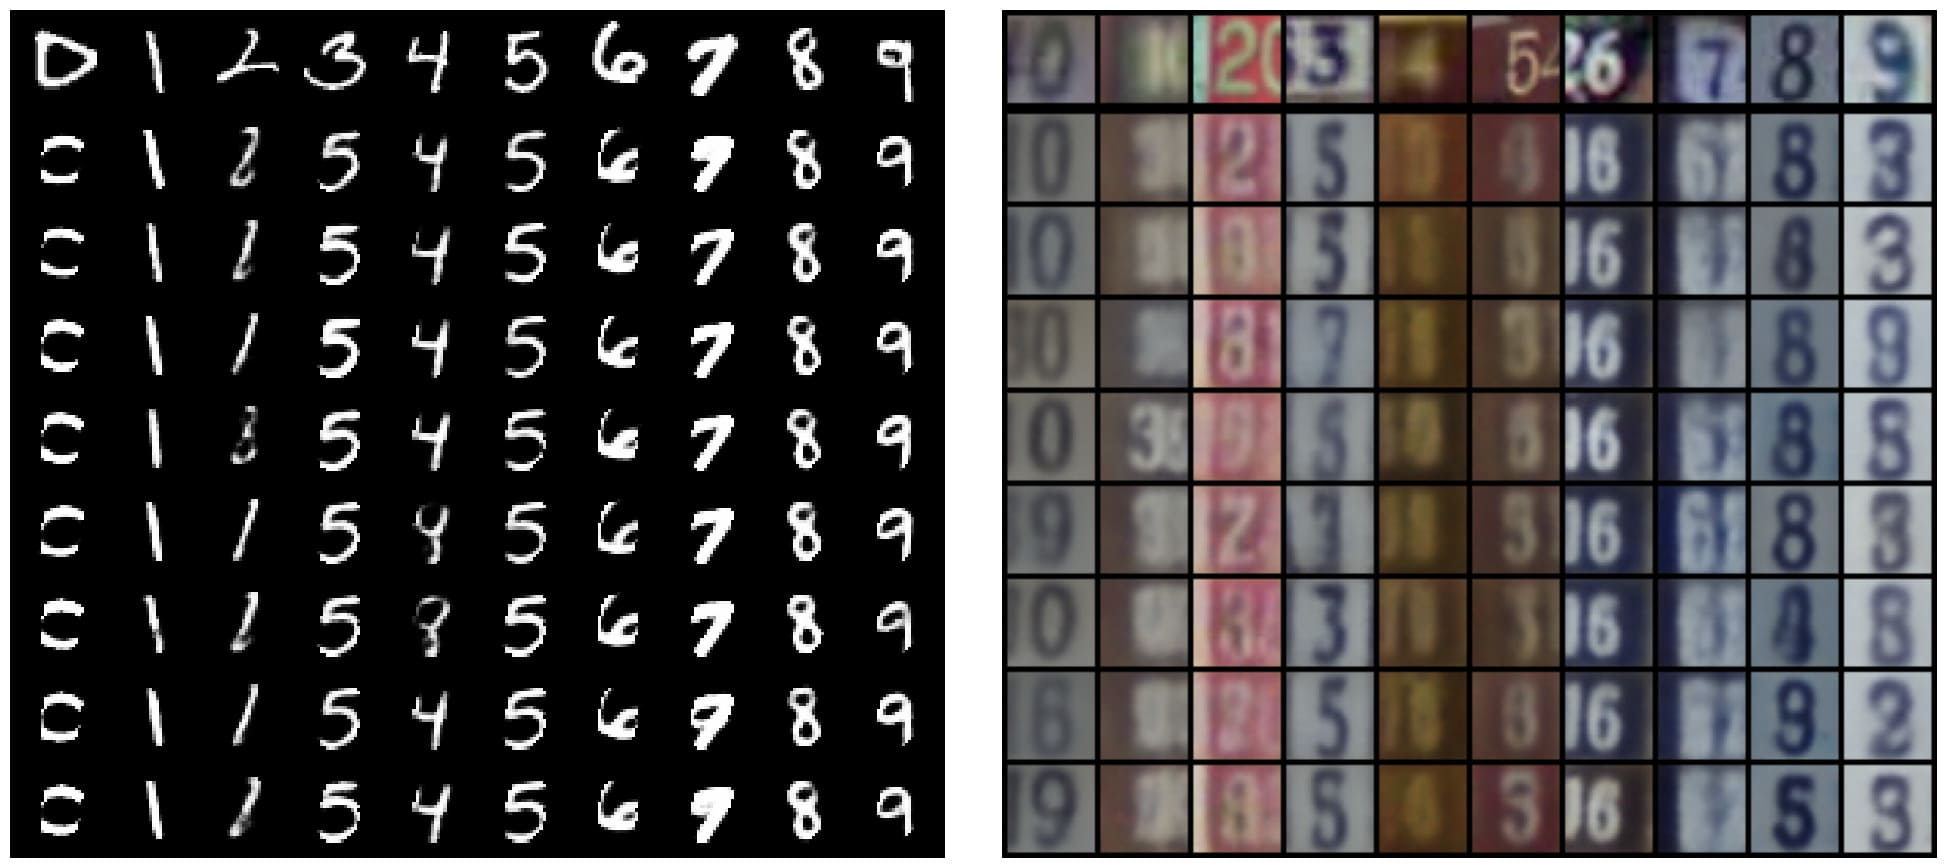
\includegraphics[width=\linewidth]{figures/datasets/ms/ms_mvae_self_recon_mnist_svhn}
         \caption*{\gls{MVAE}}
     \end{subfigure}
    \begin{subfigure}[b]{0.4\textwidth}
         \centering
         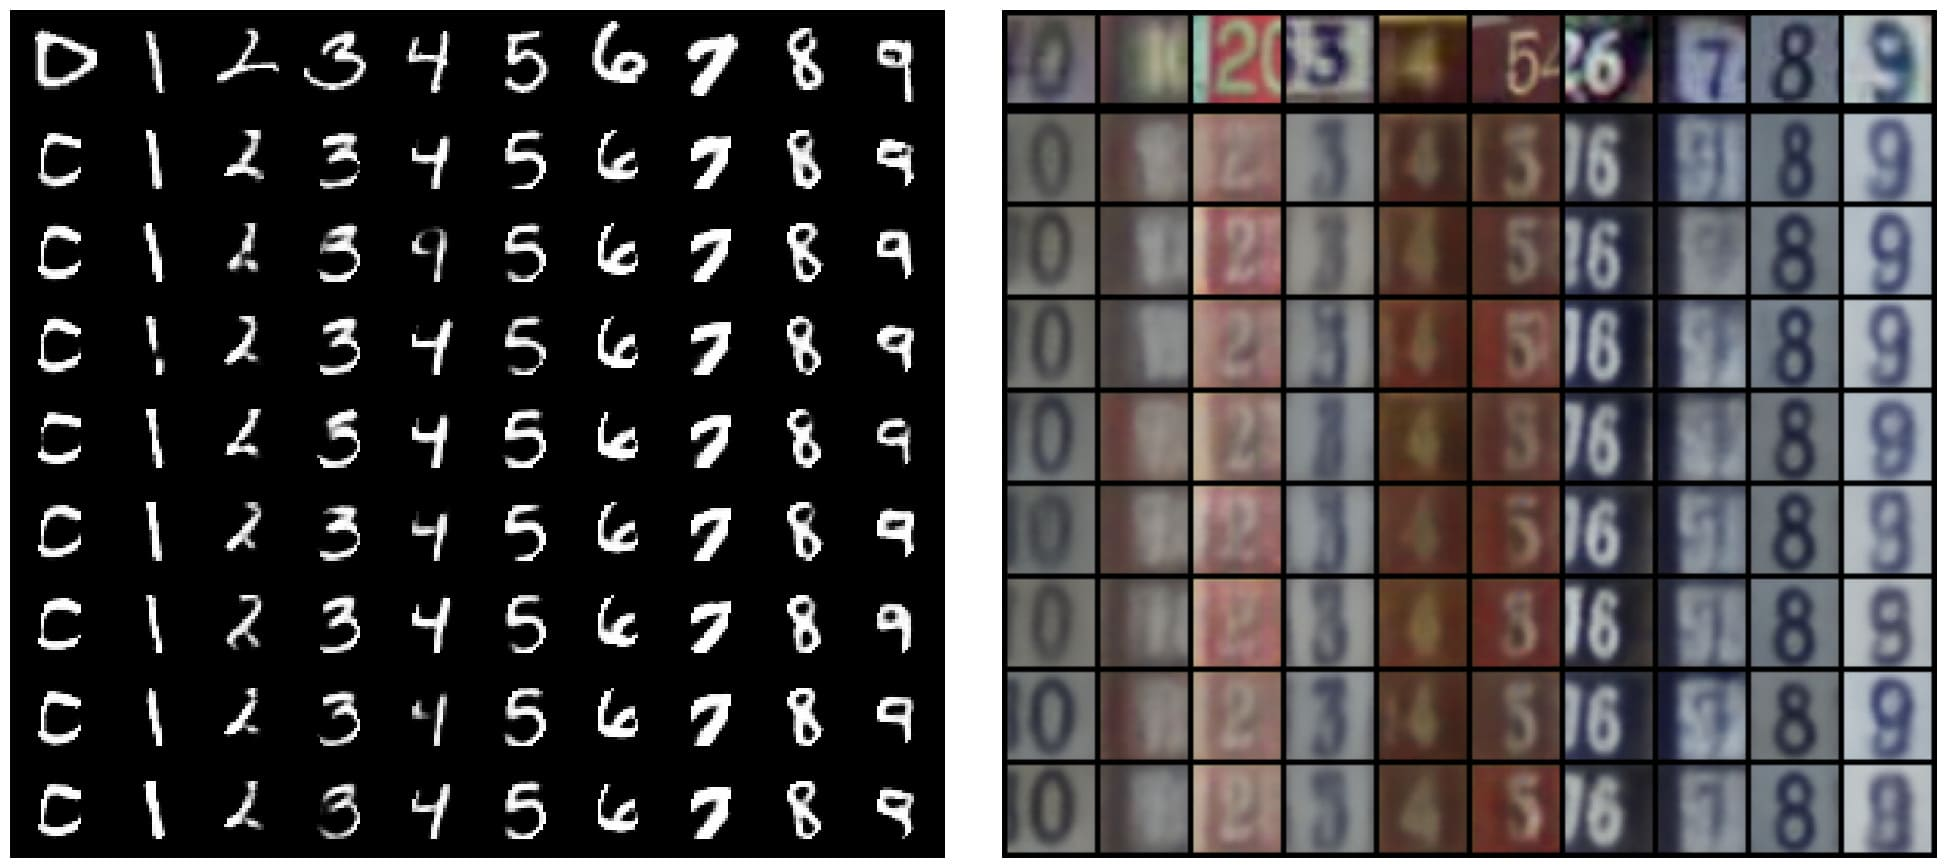
\includegraphics[width=\linewidth]{figures/datasets/ms/ms_mmvae_self_recon_mnist_svhn}
         \caption*{\gls{MMVAE}}
     \end{subfigure}
     
      \begin{subfigure}{0.4\textwidth}
         \centering
         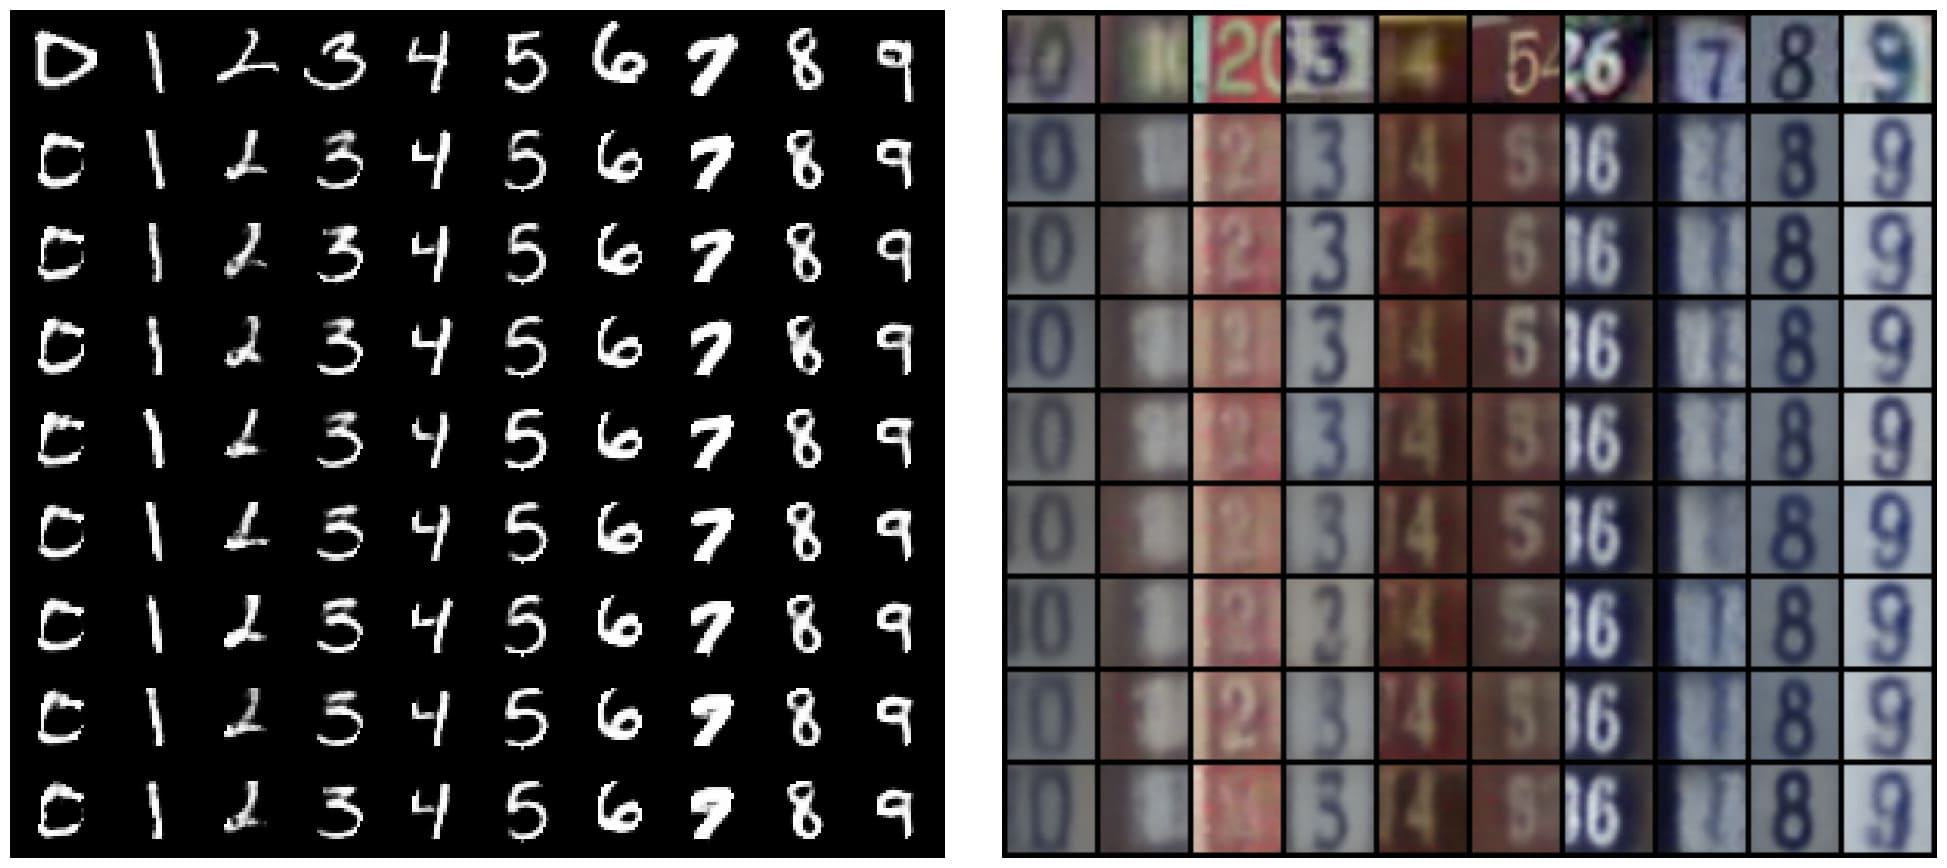
\includegraphics[width=\linewidth]{figures/datasets/ms/ms_mopoe_self_recon_mnist_svhn}
         \caption*{\gls{MOPOE}}
     \end{subfigure}
     \begin{subfigure}{0.4\textwidth}
         \centering
         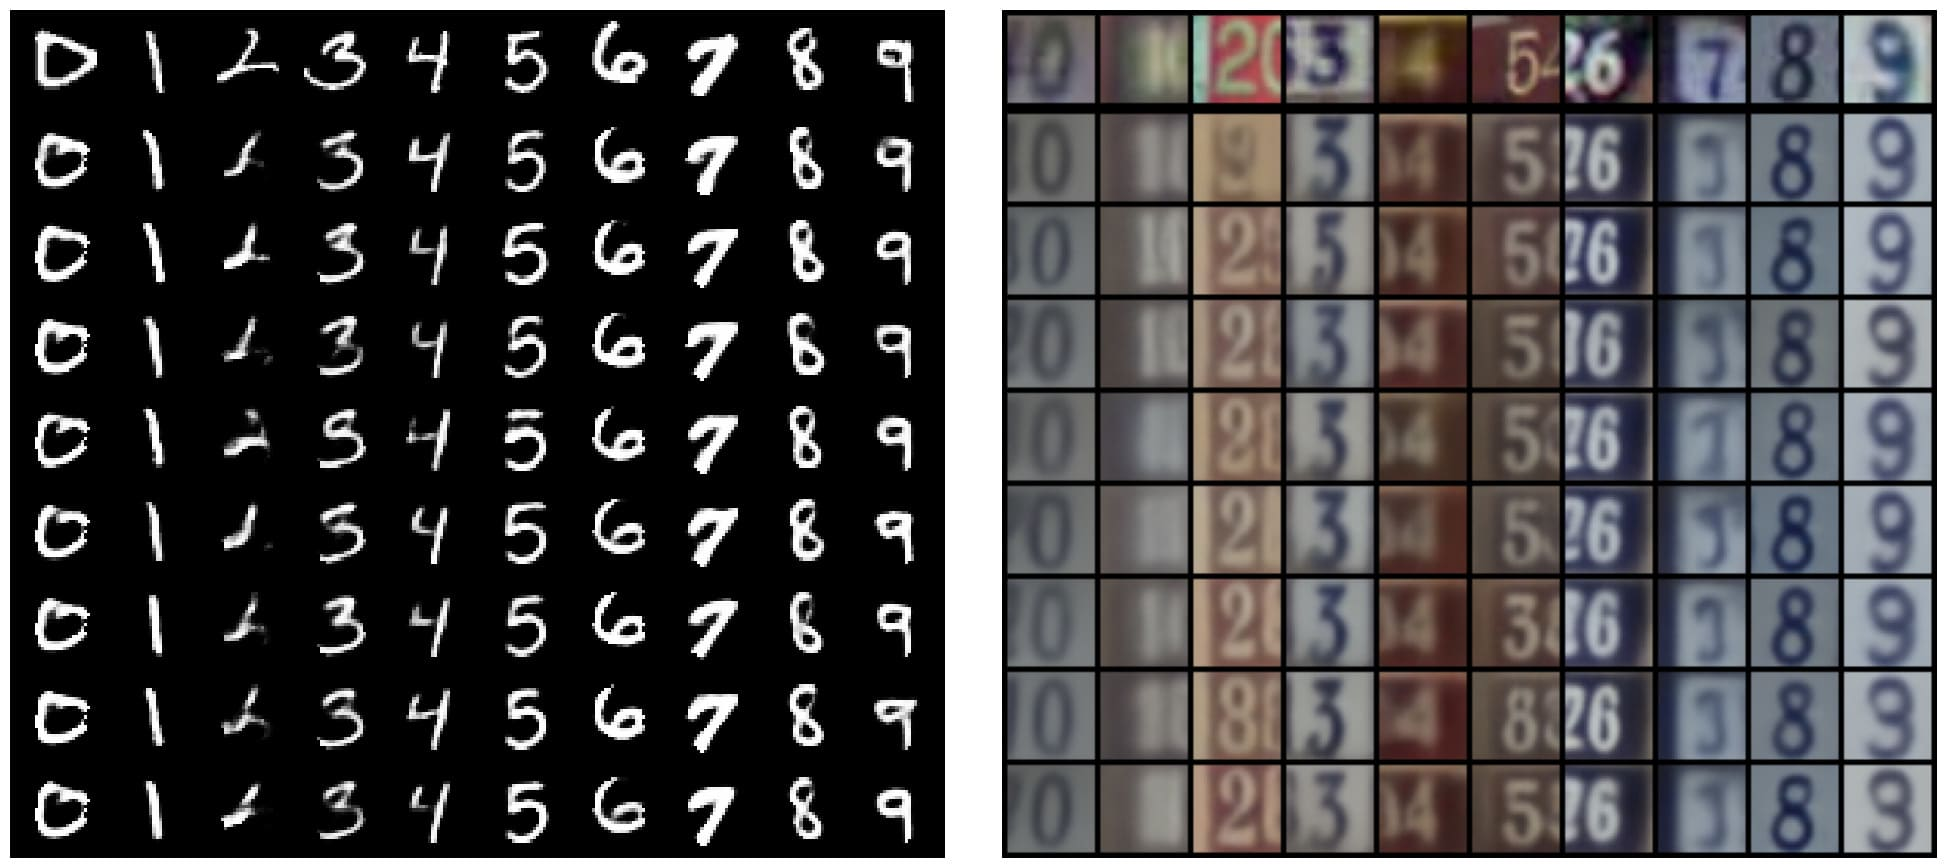
\includegraphics[width=\linewidth]{figures/datasets/ms/ms_nexus_self_recon_mnist_svhn}
         \caption*{\gls{NEXUS}}
     \end{subfigure}

    \begin{subfigure}{0.4\textwidth}
         \centering
         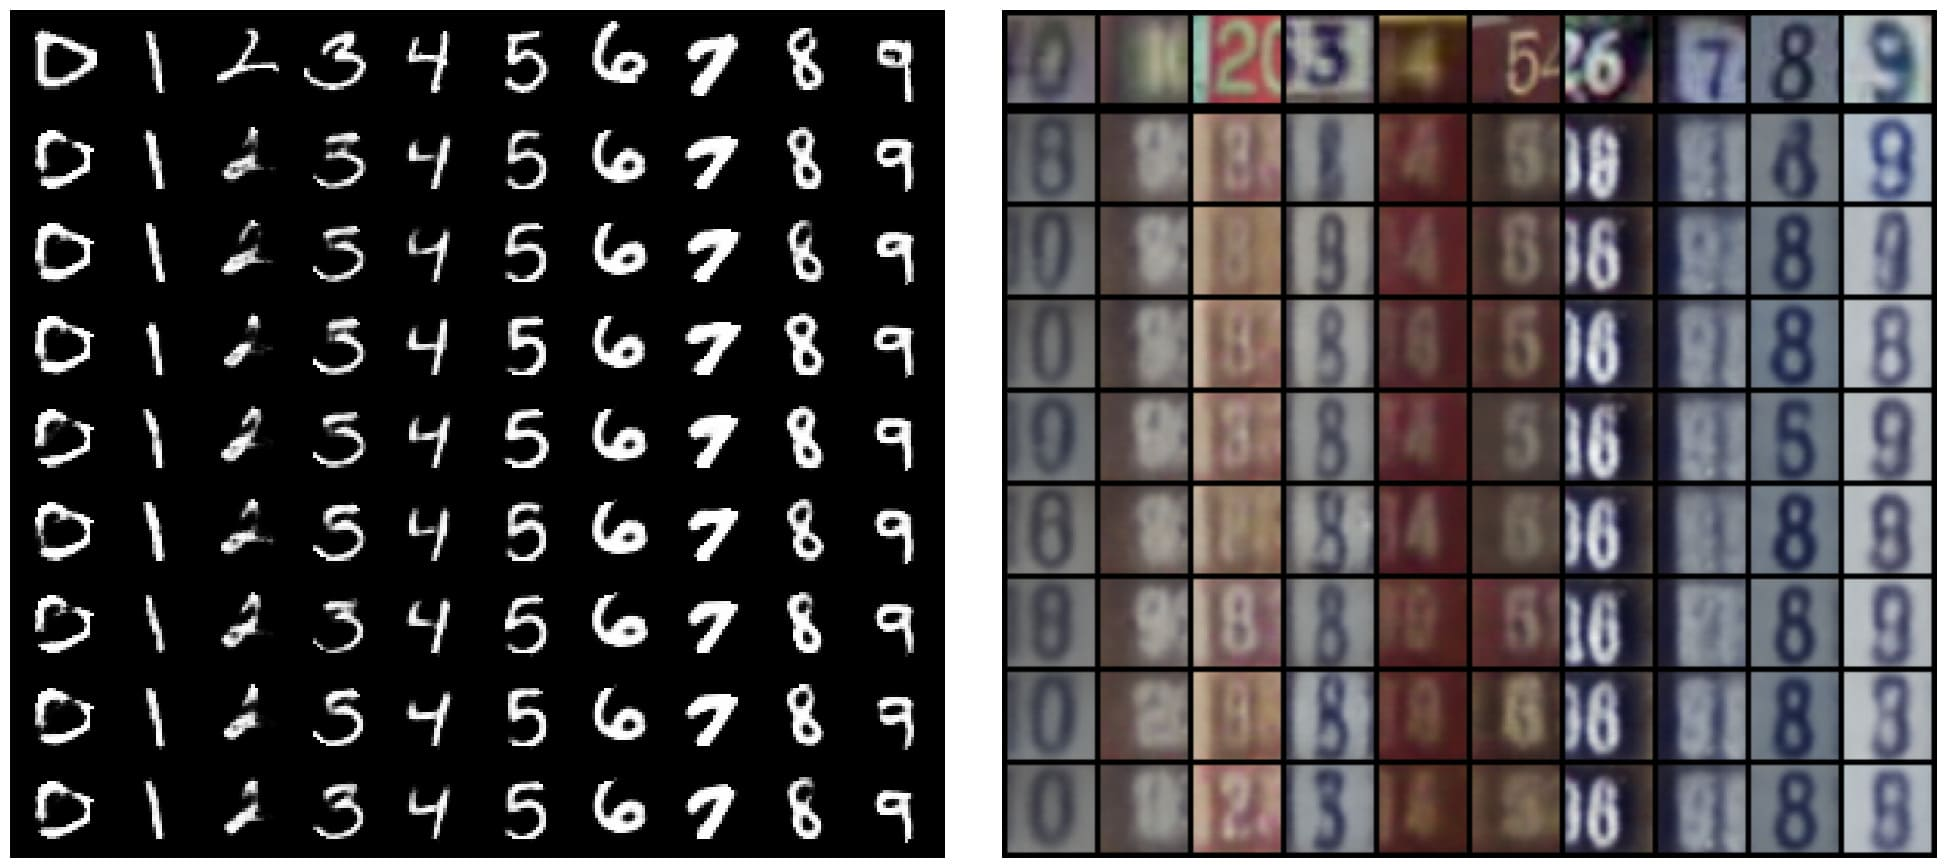
\includegraphics[width=\linewidth]{figures/datasets/ms/ms_mvtcae_self_recon_mnist_svhn}
         \caption*{\gls{MVTCAE}}
     \end{subfigure}
    \begin{subfigure}{0.4\textwidth}
         \centering
         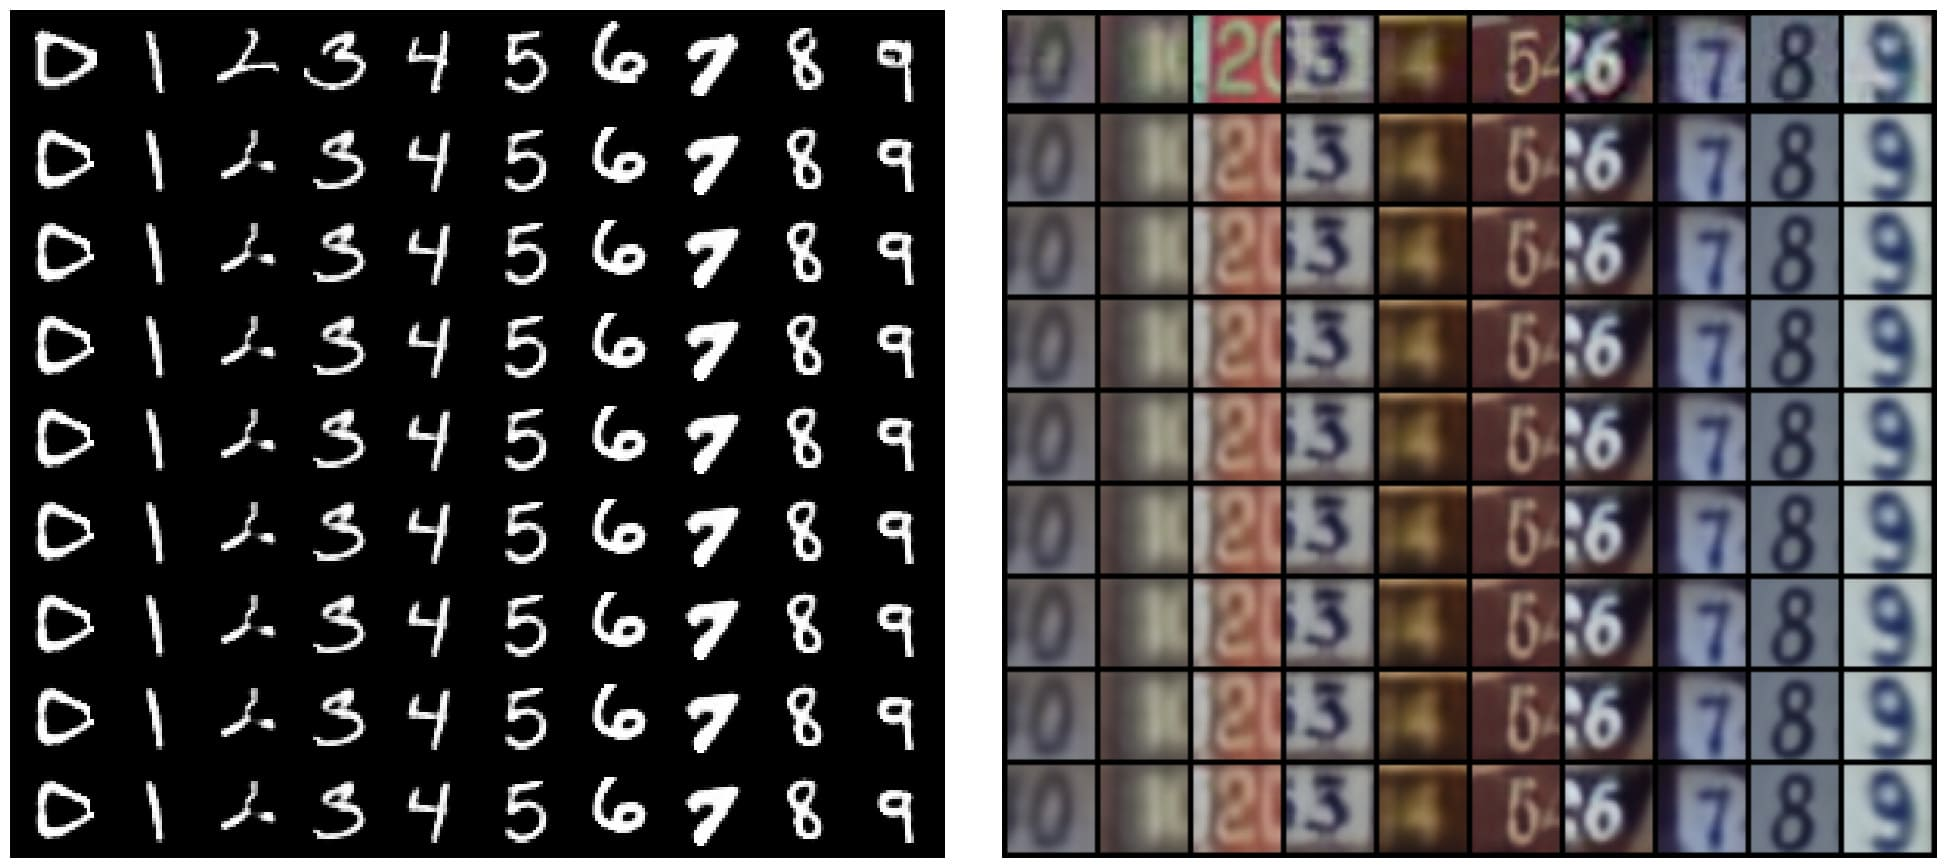
\includegraphics[page=1,width=\linewidth]{figures/datasets/ms/ms_MLD_self_recon_mnist_svhn}
         \caption*{ \textbf{\gls{MLD} (ours) }  }
     \end{subfigure}
     
        \caption{Self-generation qualitative results for \textbf{\mnist-\svhn}. For each model we report: \mnist to \mnist conditional generation in the left,   \svhn to \svhn conditional generation in the right. \newline }
        \label{fig:self_recon}
\end{figure}

\subsubsection{Detailed results}


\begin{table}[h]
\centering
\caption{Generative Coherence for \textbf{\mnist-\svhn}. We report the detailed version of \Cref{coh_quality:ms} with standard deviation for 5 independent runs with different seeds.\newline}
 \label{coh_quality:ms_detailed}
\resizebox{\textwidth}{!}{\begin{tabular}{c|c|cc|cc|cc}
\toprule
\multirow{2}{*}{ Models }  & \multicolumn{3}{c}{Coherence (\%$\uparrow$) } &   \multicolumn{4}{c}{Quality ($\downarrow$)} \\
    \cmidrule{2-8}
    & Joint &  M $\rightarrow$ S & S $\rightarrow$ M &
     Joint(M)  &  Joint(S) &M $\rightarrow$ S &  S $\rightarrow$ M  \\
    \midrule
     \gls{MVAE} &  
     $38.19_{ \pm 2.27 }$ &
     $48.21_{\pm 2.56 }$  &
     $ 28.57_{\pm 1.46}$ & 
     $13.34_{ \pm 0.93}$ &
     $68.0_{\pm 0.99}$   & 
     $ 68.9_{\pm 1.84}  $ &
     $ 13.66_{\pm 0.95} $ 
    
     \\
    \gls{MMVAE} &  $37.82_{ \pm 1.19 }$ & $11.72_{\pm 0.33 }$ & $ 67.55_{\pm 9.22}$ & $25.89_{ \pm 0.46}$ &
    $ 146.82_{\pm 4.76}  $& $393.33_{\pm 4.86}$  &
    $ 53.37_{\pm 1.87} $ 
 
    \\
    \gls{MOPOE} & $ 39.93_{ \pm 1.54 }$ & $12.27_{\pm 0.68 }$ & $68.82_{\pm 0.39}$ &$20.11_{ \pm 0.96}$ &
    $ 129.2_{\pm 6.33}  $&$373.73_{\pm26.42}$&
    $ 43.34_{\pm 1.72} $
        \\

    \gls{NEXUS} &  $ 40.0_{ \pm 2.74 }$ & $16.68_{\pm 5.93 }$ & $70.67_{\pm 0.77}$ &  $13.84_{ \pm 1.41}$ &
        $ 98.13_{\pm 5.9}  $ &$281.28_{\pm16.07}$&
 $ 53.41_{\pm 1.54} $
   \\


    \gls{MVTCAE} & $48.78_{ \pm 1 } $& $\underline{81.97}_{\pm 0.32 }$ & $49.78_{\pm 0.88} $&$12.98_{ \pm 0.68}$ &
    $ \textbf{52.92}_{\pm 1.39}  $&$69.48_{\pm1.64}$ &
    $ 13.55_{\pm 0.8} $ 

     \\ 
\gls{MMVAEplus} & $17.64_{ \pm 4.12 }$ &$13.23_{ \pm 4.96 }$ & $29.69_{ \pm 5.08 }$ 
&$26.60_{ \pm 2.58 }$ & $121.77_{ \pm 37.77 }$ 
& $240.90_{ \pm 85.74 }$
&$35.11_{ \pm 4.25 }$
\\
  \gls{MMVAEplus}(K=10) & $41.59_{ \pm 4.89 }$ & $55.3_{ \pm 9.89 }$
& $56.41_{ \pm 5.37 }$ & $19.05_{ \pm 1.10 }$ & $67.13_{ \pm 4.58 }$ & $75.9_{ \pm 12.91 }$ & $18.16_{ \pm 2.20 }$
\\
    \midrule
    \gls{MLD}  & $\underline{85.22}_{ \pm 0.5}$ & $\textbf{83.79}_{\pm 0.62} $&$ \textbf{79.13}_{\pm 0.38}$ & $\underline{3.93}_{ \pm 0.12}$ &
    $\underline{56.36}_{\pm1.63}$   &
    $\textbf{	57.2}_{\pm1.47}$  &
    $\underline{3.67}_{\pm 0.14} $ 
    \\
    
    \bottomrule
\end{tabular}}
\end{table}

















\begin{figure}[H]
     \centering
       \centering
     \begin{subfigure}{0.40\textwidth}
         \centering
         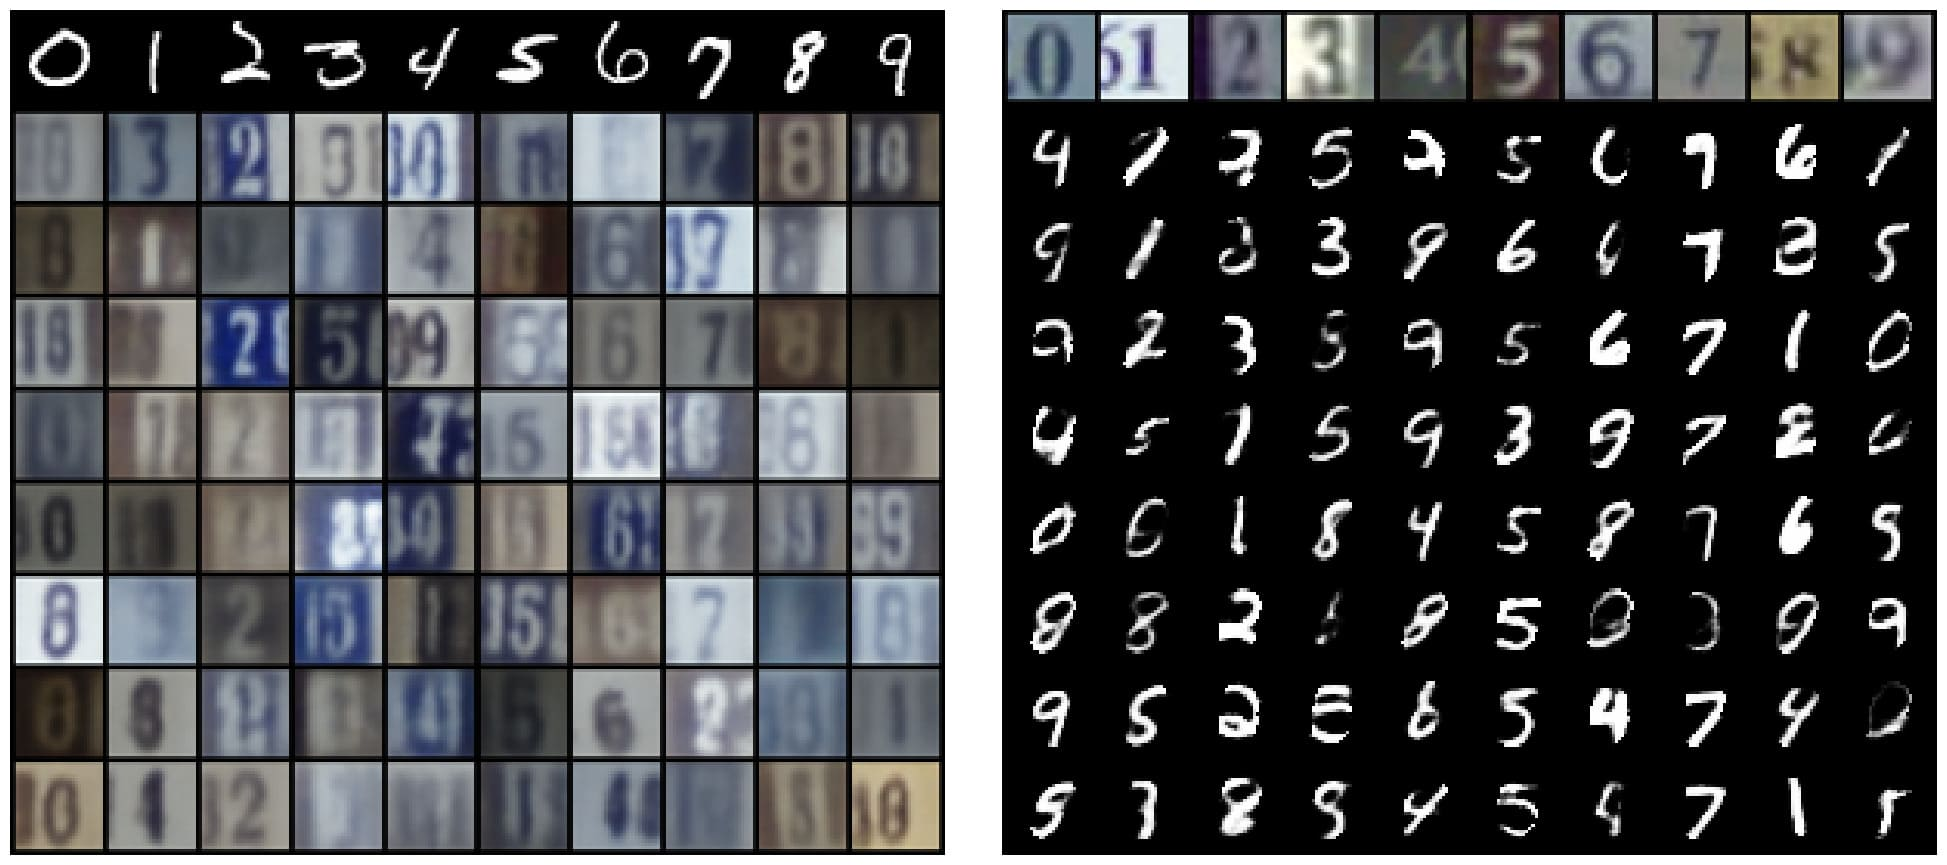
\includegraphics[width=\linewidth]{figures/datasets/ms/ms_mvae_cond_mnist_svhn}
         \caption*{\gls{MVAE}}
    
     \end{subfigure}
     \begin{subfigure}{0.40\textwidth}
         \centering
         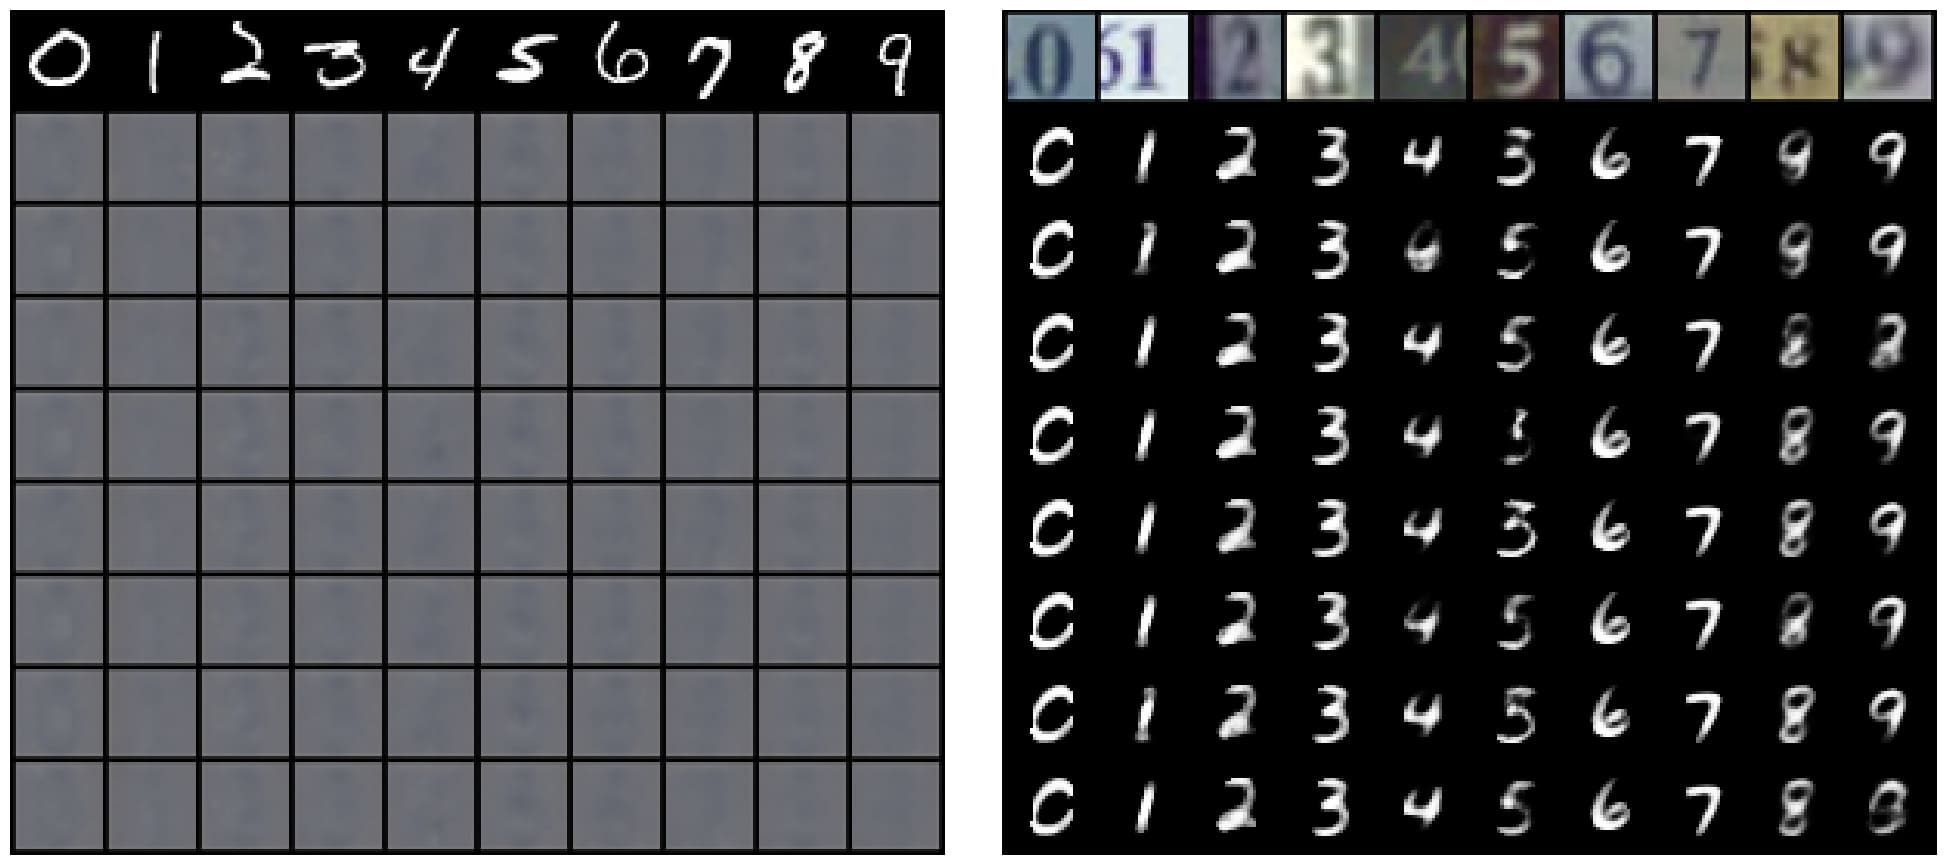
\includegraphics[width=\linewidth]{figures/datasets/ms/ms_mmvae_cond_mnist_svhn}
         \caption*{\gls{MMVAE}}
      
     \end{subfigure}
     
       \begin{subfigure}{0.40\textwidth}
         \centering
         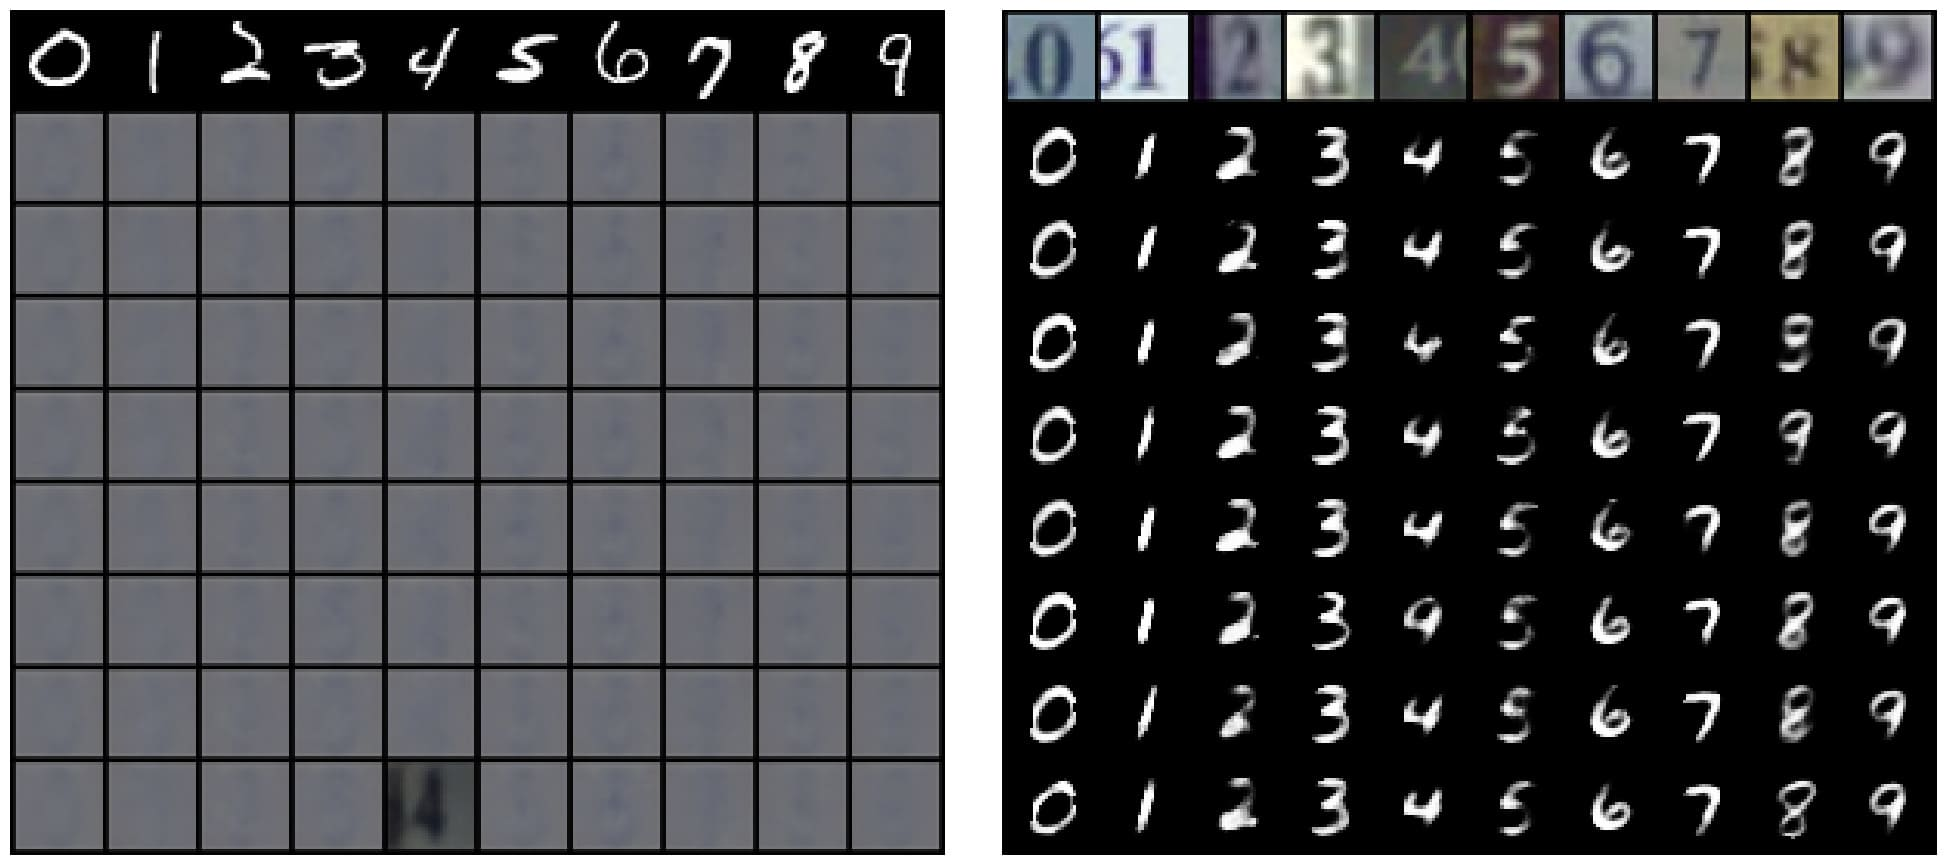
\includegraphics[width=\linewidth]{figures/datasets/ms/ms_mopoe_cond_mnist_svhn}
         \caption*{\gls{MOPOE}}
     
     \end{subfigure}
      \begin{subfigure}{0.40\textwidth}
         \centering
         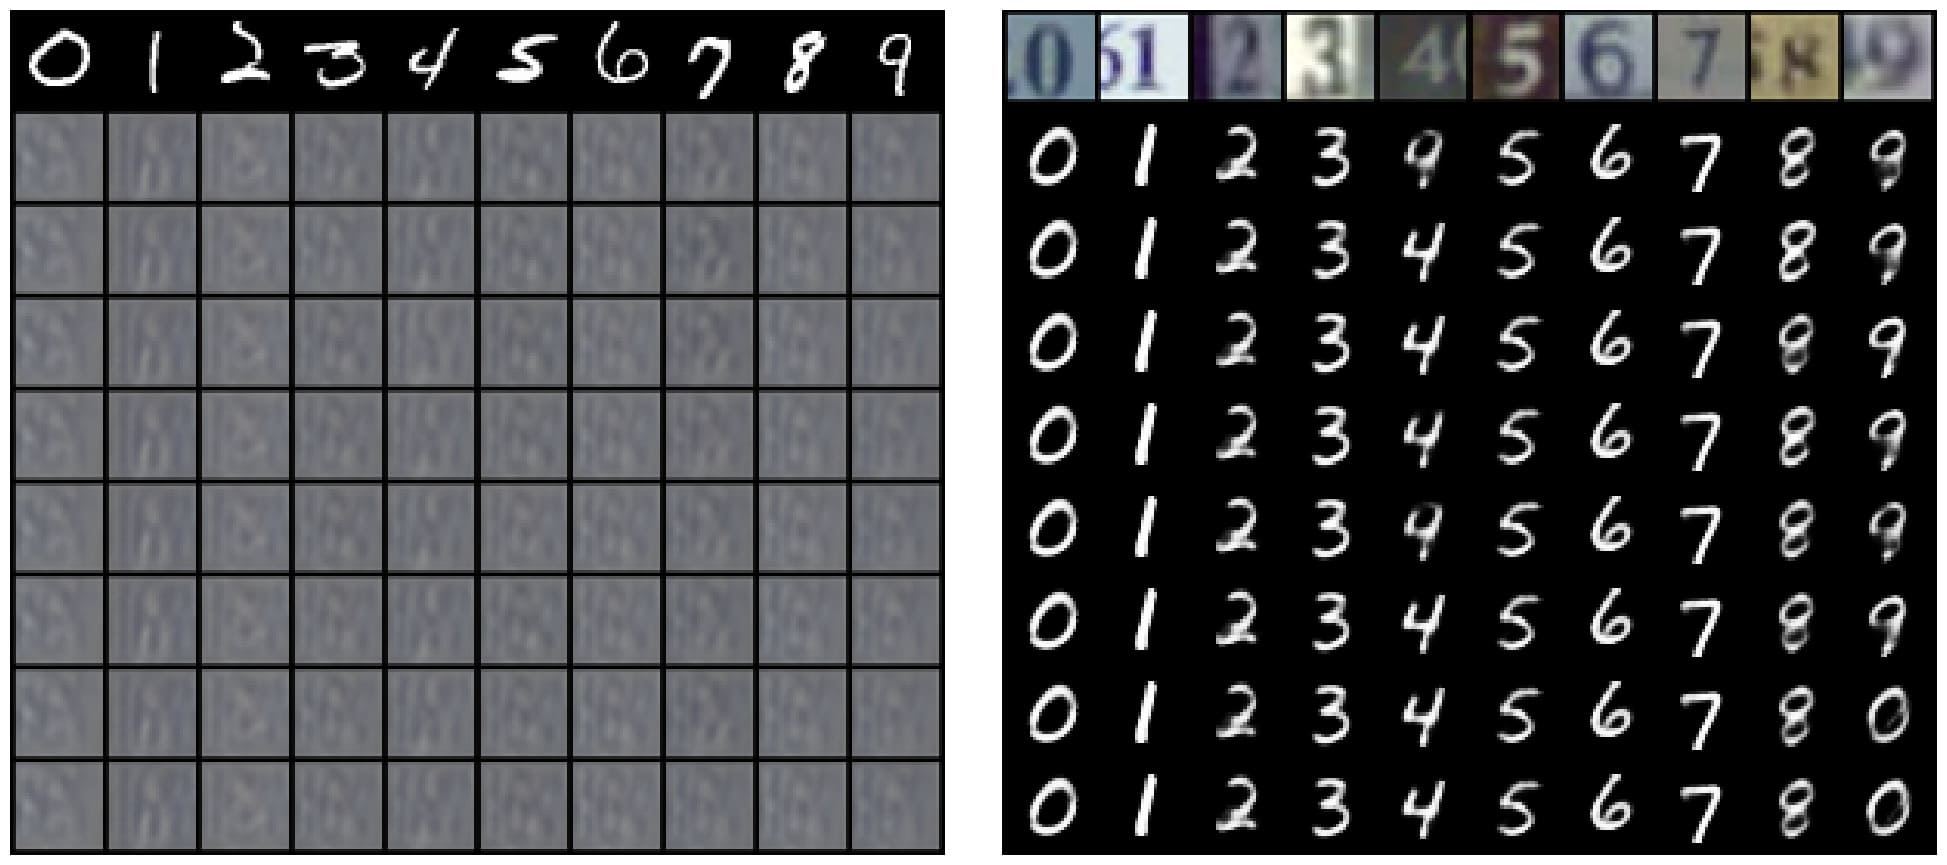
\includegraphics[width=\linewidth]{figures/datasets/ms/ms_nexus_cond_mnist_svhn}
         \caption*{\gls{NEXUS}}
   
     \end{subfigure}
     
  \begin{subfigure}{0.40\textwidth}
         \centering
         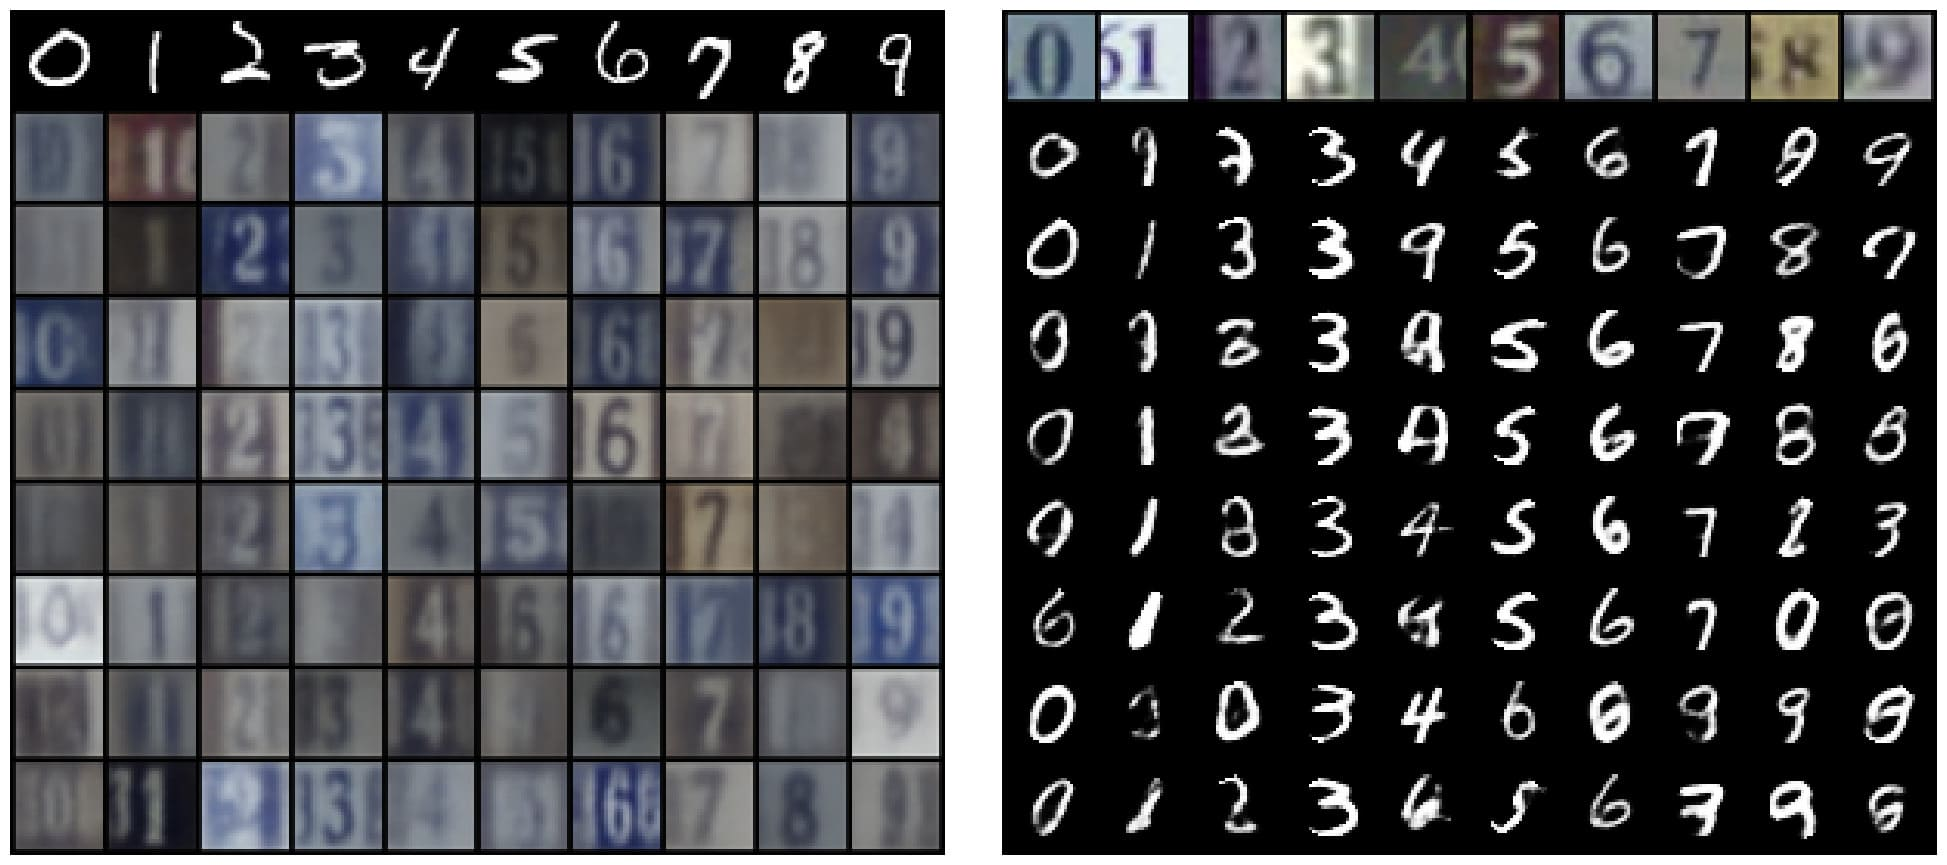
\includegraphics[width=\linewidth]{figures/datasets/ms/ms_mvtcae_cond_mnist_svhn}
         \caption*{\gls{MVTCAE}}
      
     \end{subfigure}
\begin{subfigure}{0.40\textwidth}
         \centering
         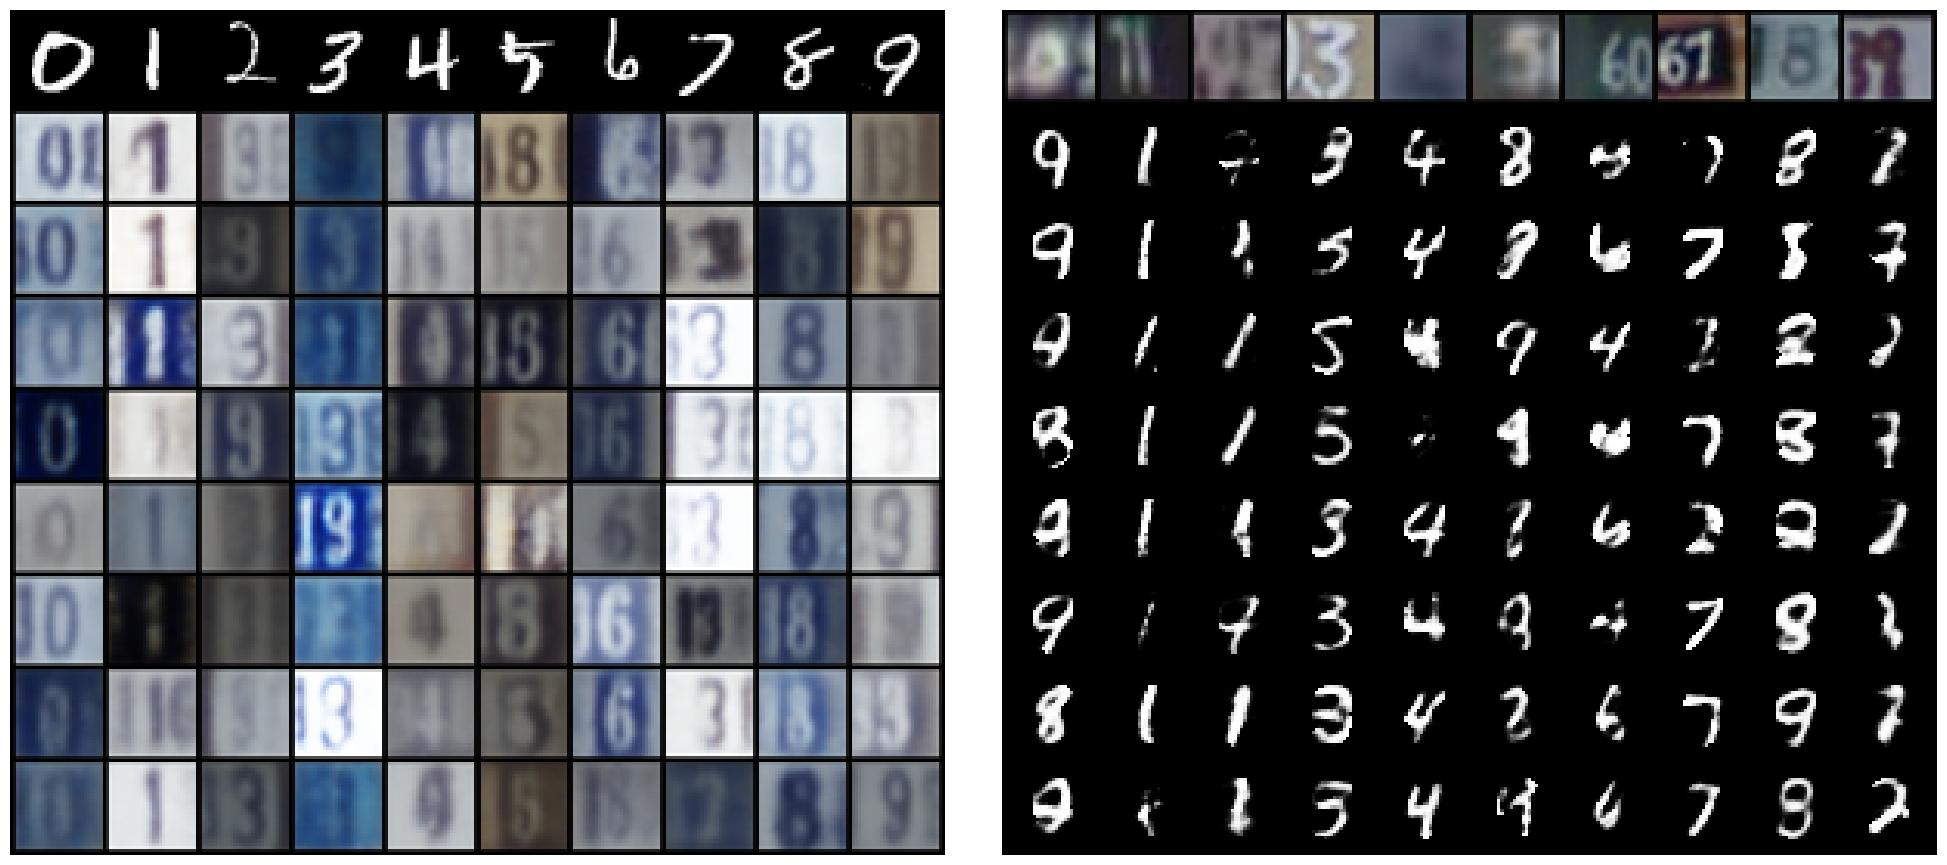
\includegraphics[width=\linewidth]{figures/datasets/ms/ms_mmvae+_cond_mnist_svhn.jpg}
         \caption*{\gls{MMVAEplus}(K=10)}
      
     \end{subfigure}
     
  \begin{subfigure}{0.40\textwidth}
         \centering
         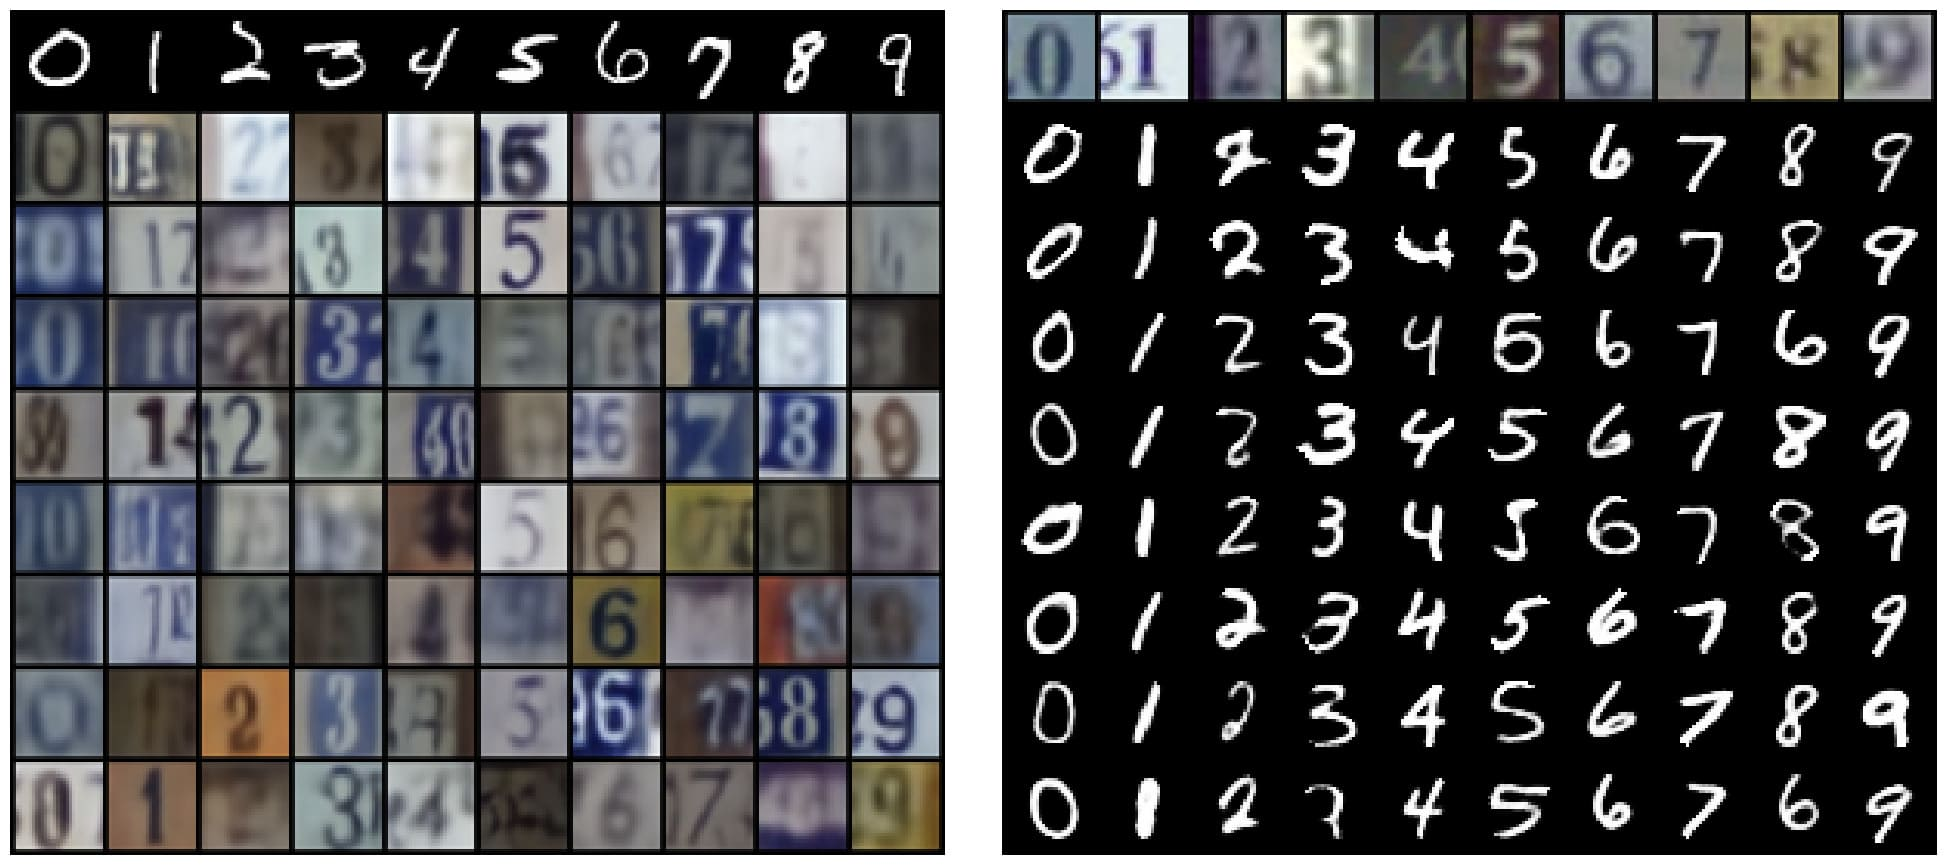
\includegraphics[page=1,width=\linewidth]{figures/datasets/ms/ms_MLD_cond_mnist_svhn}
         \caption*{\textbf{\gls{MLD} (ours) }  }
     
     \end{subfigure}
     
        \caption{Additional qualitative results for \textbf{\mnist-\svhn}. For each model we report: \mnist to \svhn conditional generation in the left,   \svhn to \mnist conditional generation in the right. }
        \label{fig:cond_ms_detailed}
\end{figure}

\newpage



\begin{figure}[h]
     \centering
     \begin{subfigure}{0.40\textwidth}
         \centering
         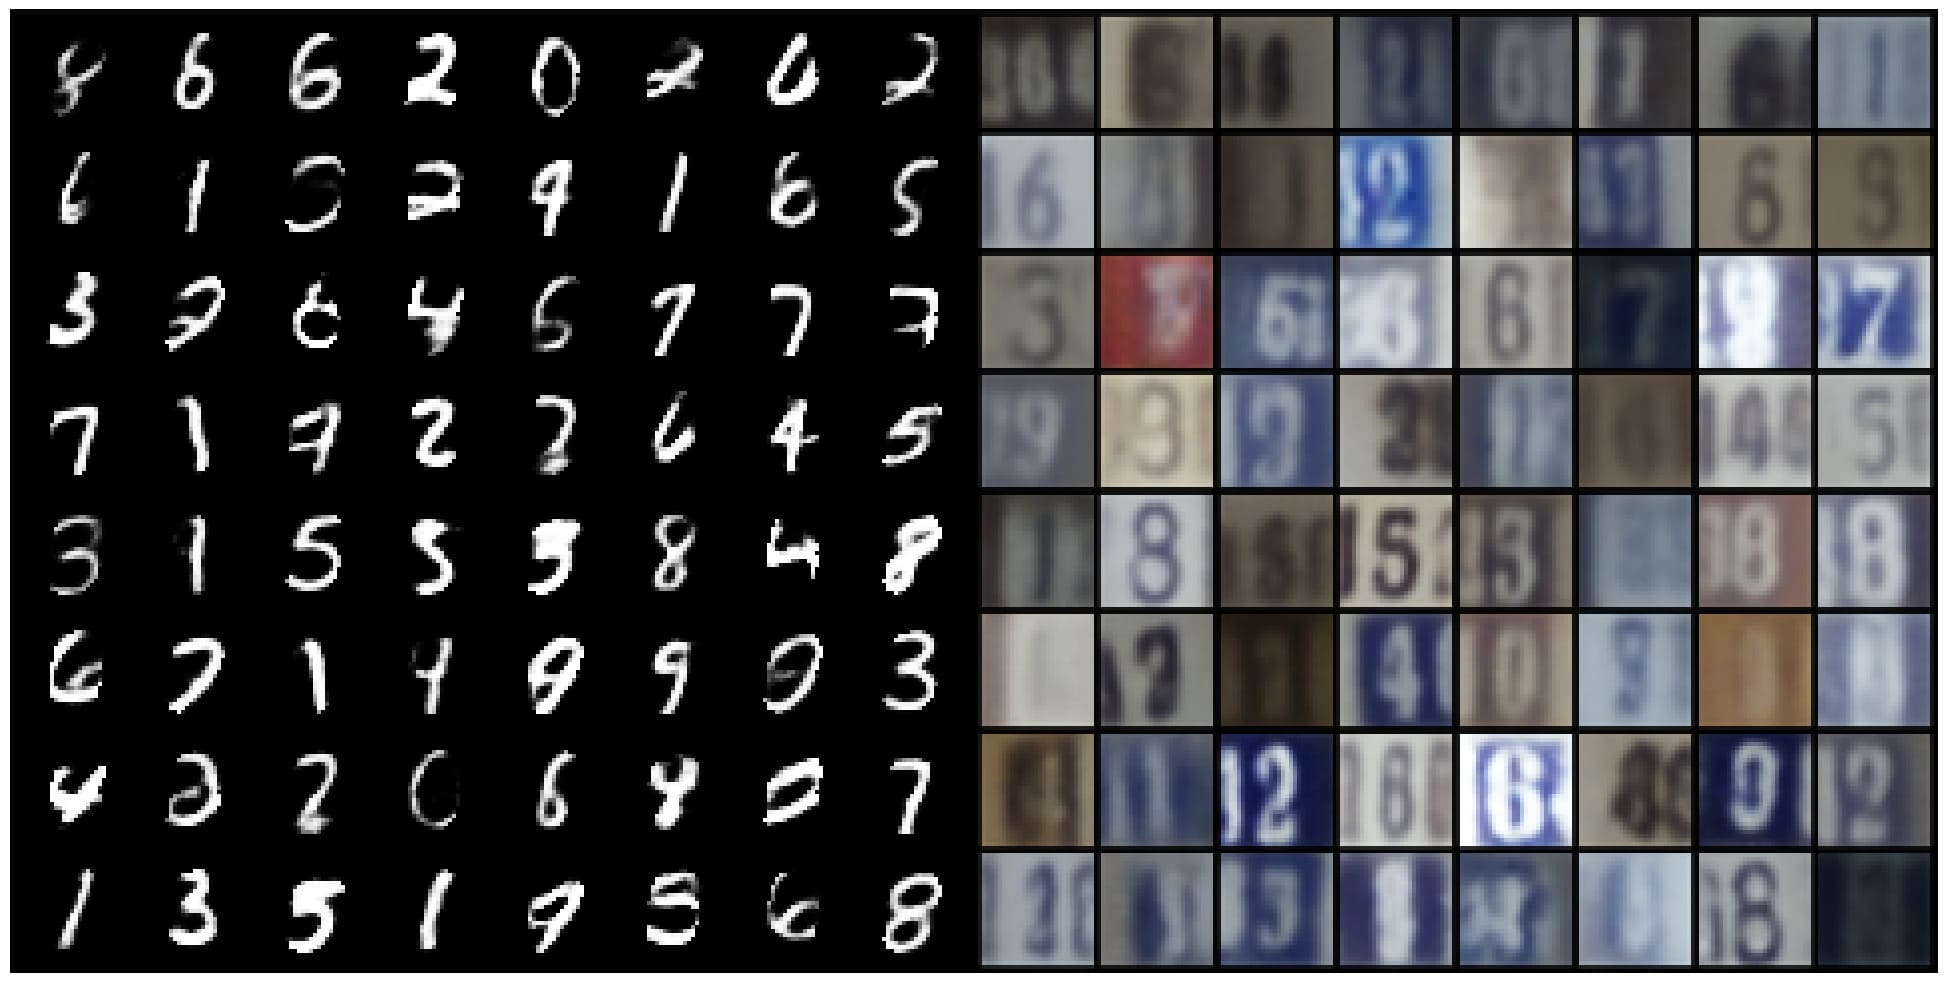
\includegraphics[width=\linewidth]{figures/datasets/ms/mvae_sampling_mnist_svhn}
  
     \caption*{\gls{MVAE}}
     \end{subfigure}
     \begin{subfigure}{0.40\textwidth}
         \centering
         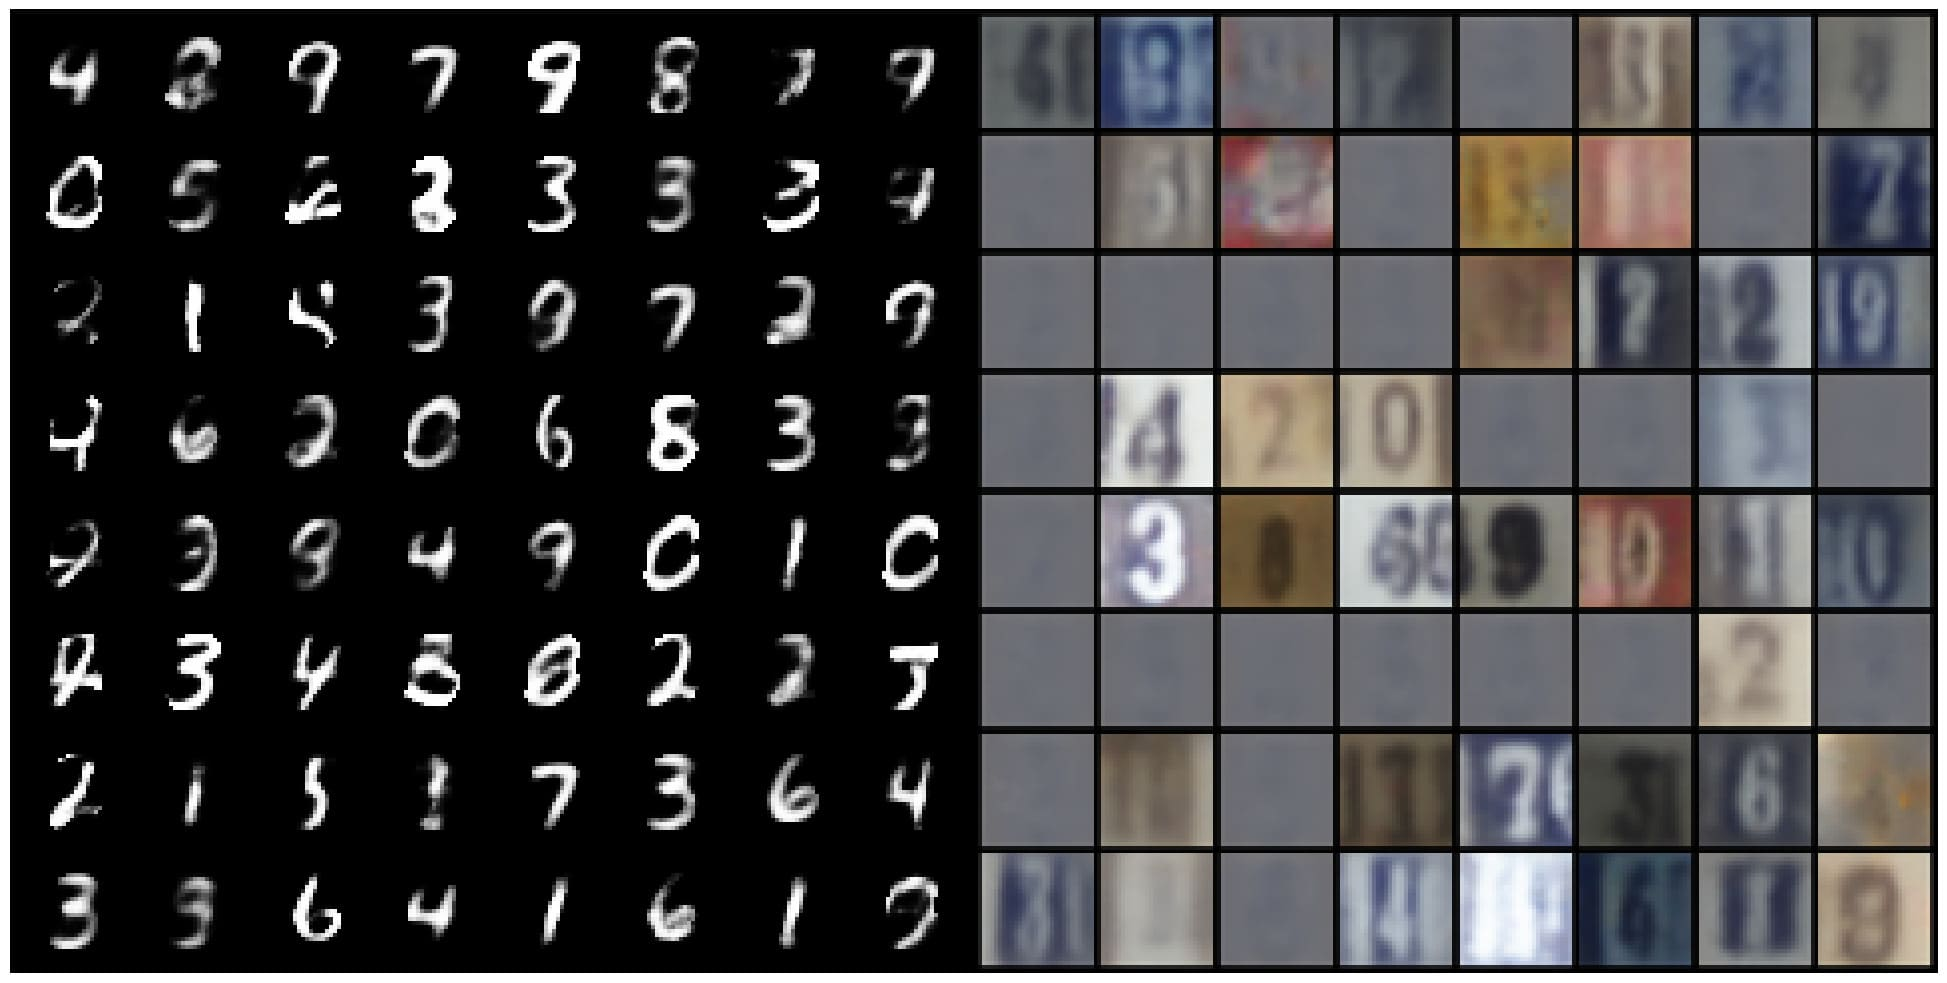
\includegraphics[width=\linewidth]{figures/datasets/ms/mmvae_sampling_mnist_svhn}
        \caption*{\gls{MMVAE}}
     \end{subfigure}
     
       \begin{subfigure}{0.40\textwidth}
         \centering
         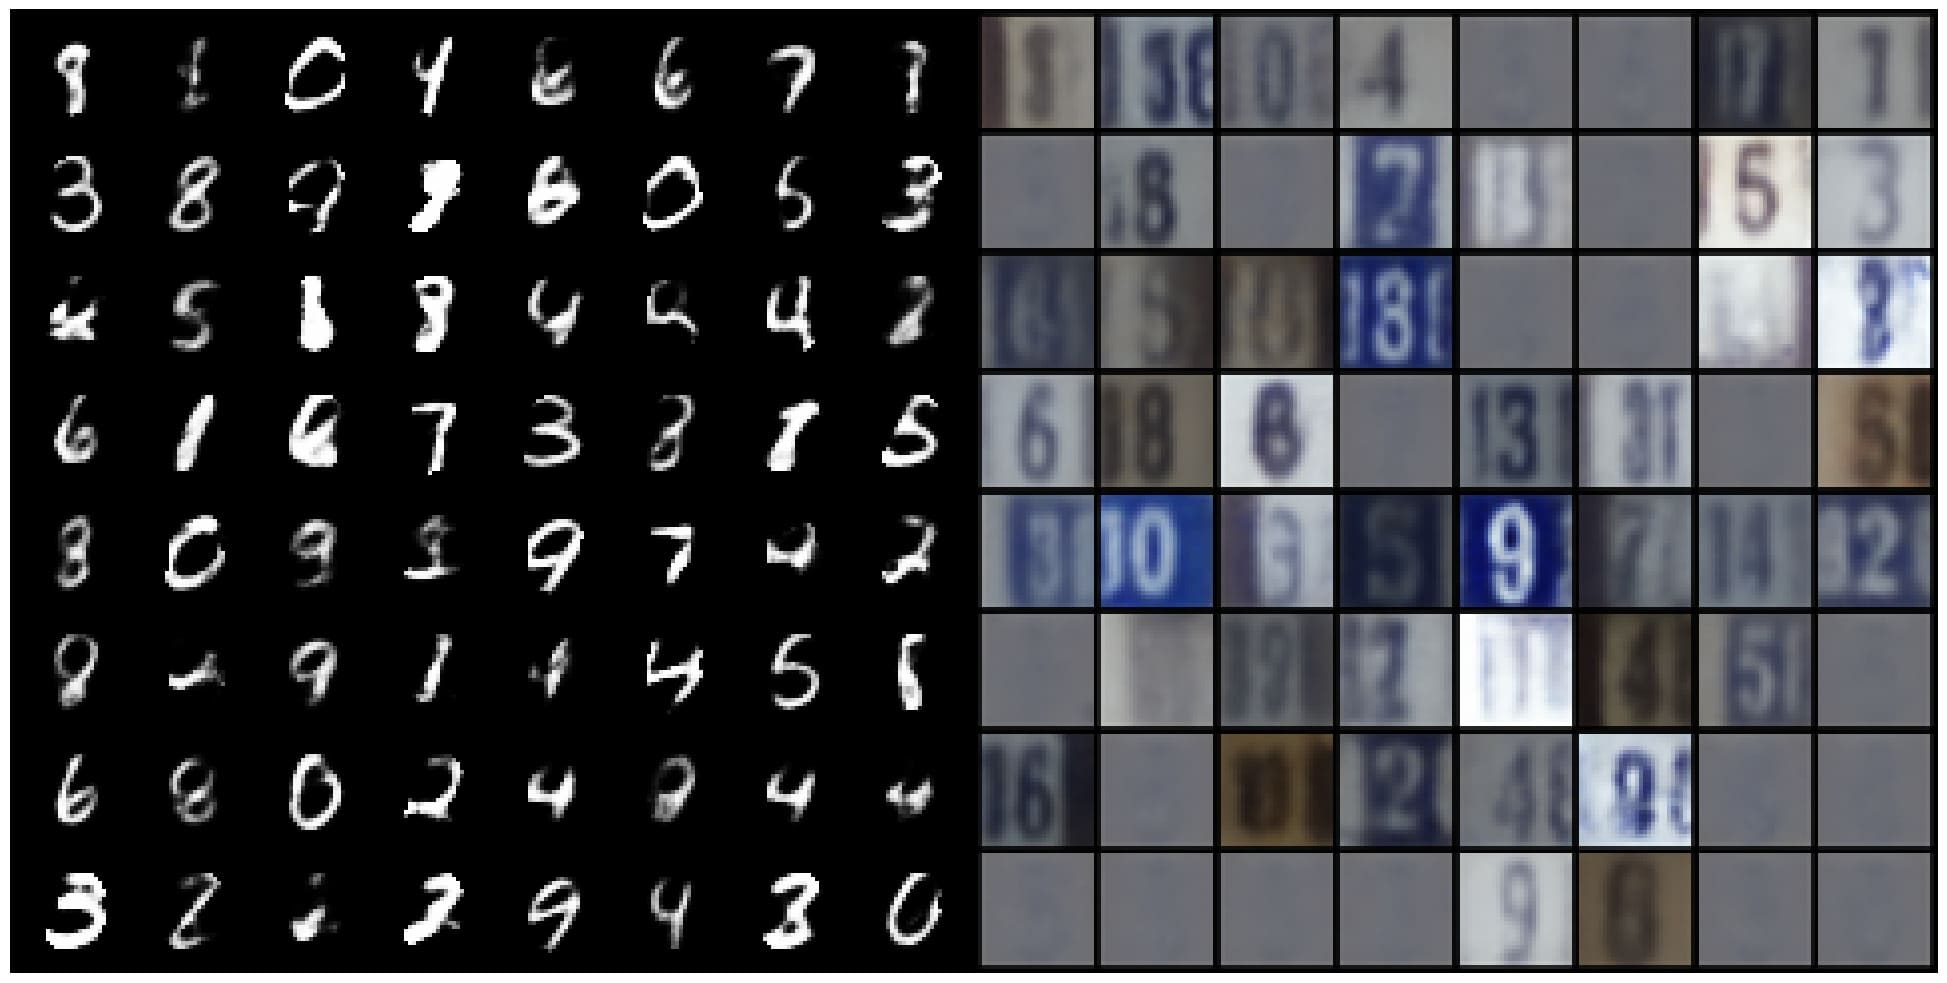
\includegraphics[width=\linewidth]{figures/datasets/ms/mopoe_sampling_mnist_svhn}
  
            \caption*{\gls{MOPOE}}
     \end{subfigure}
      \begin{subfigure}{0.40\textwidth}
         \centering
         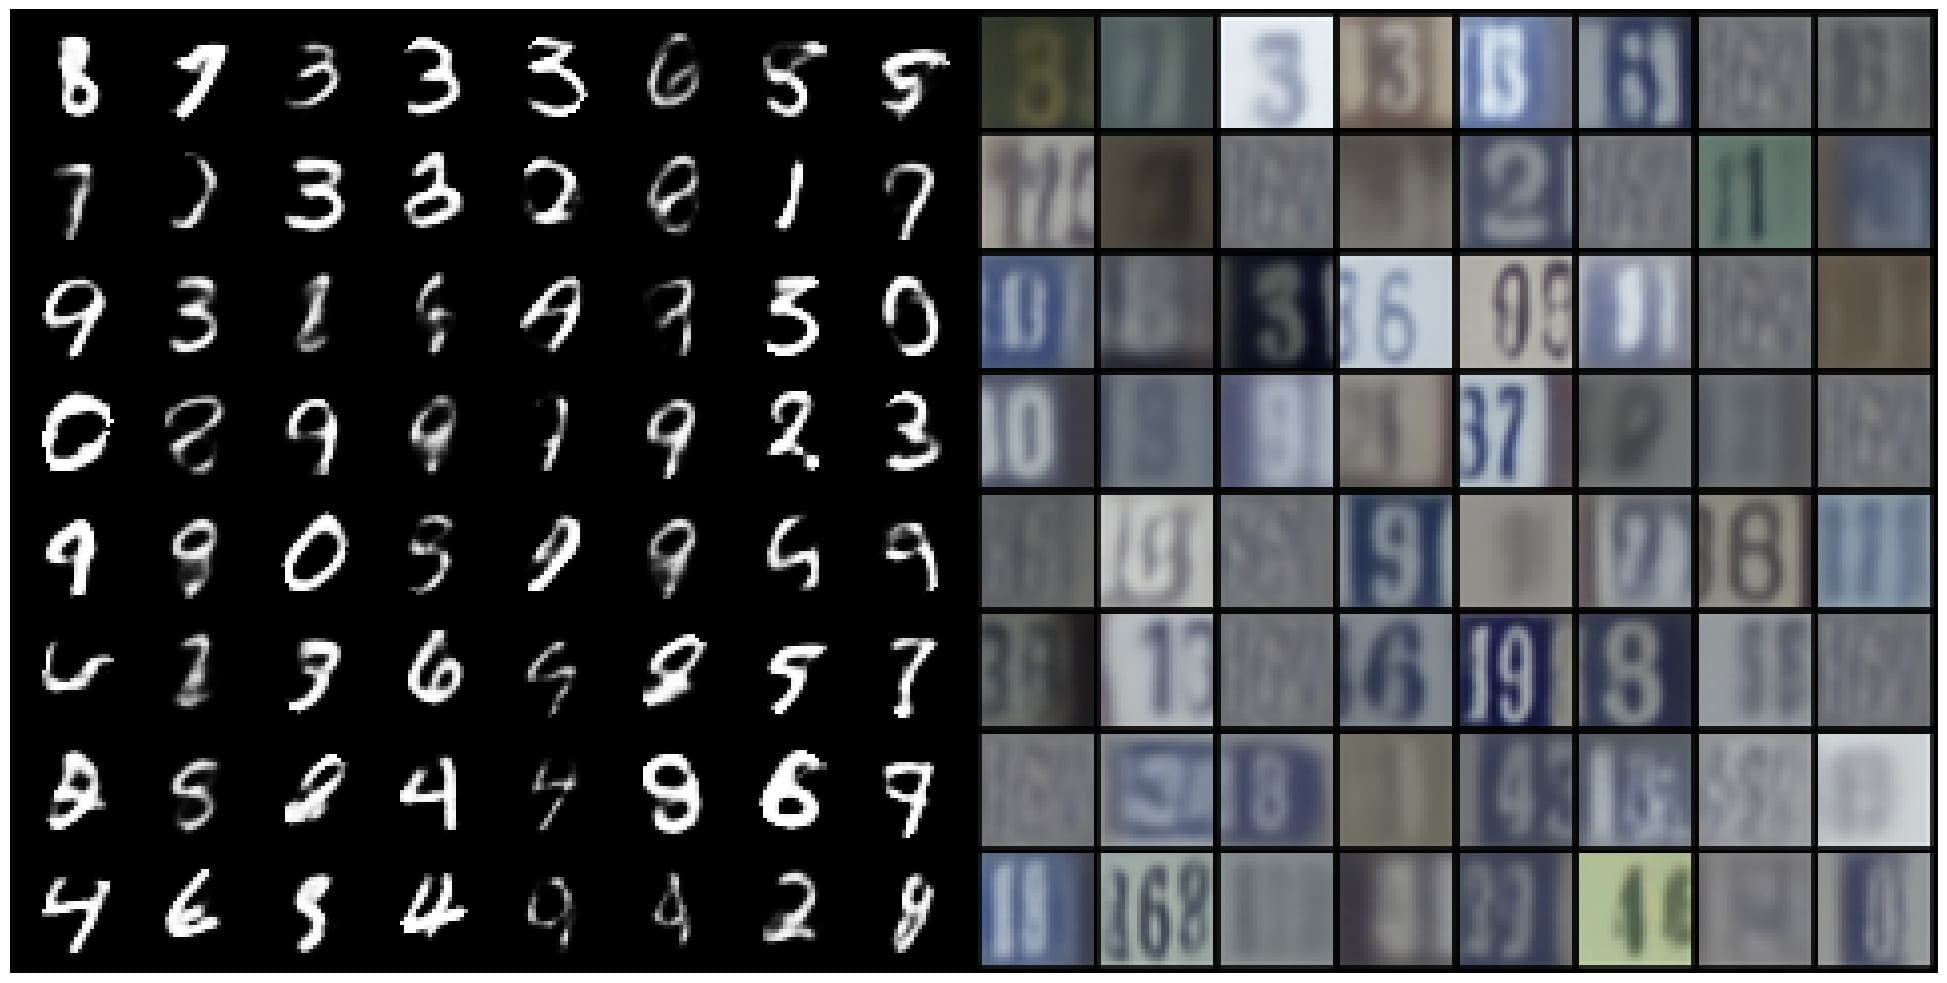
\includegraphics[width=\linewidth]{figures/datasets/ms/nexus_sampling_mnist_svhn}
         \caption*{\gls{NEXUS}}
     \end{subfigure}
     
  \begin{subfigure}{0.40\textwidth}
         \centering
         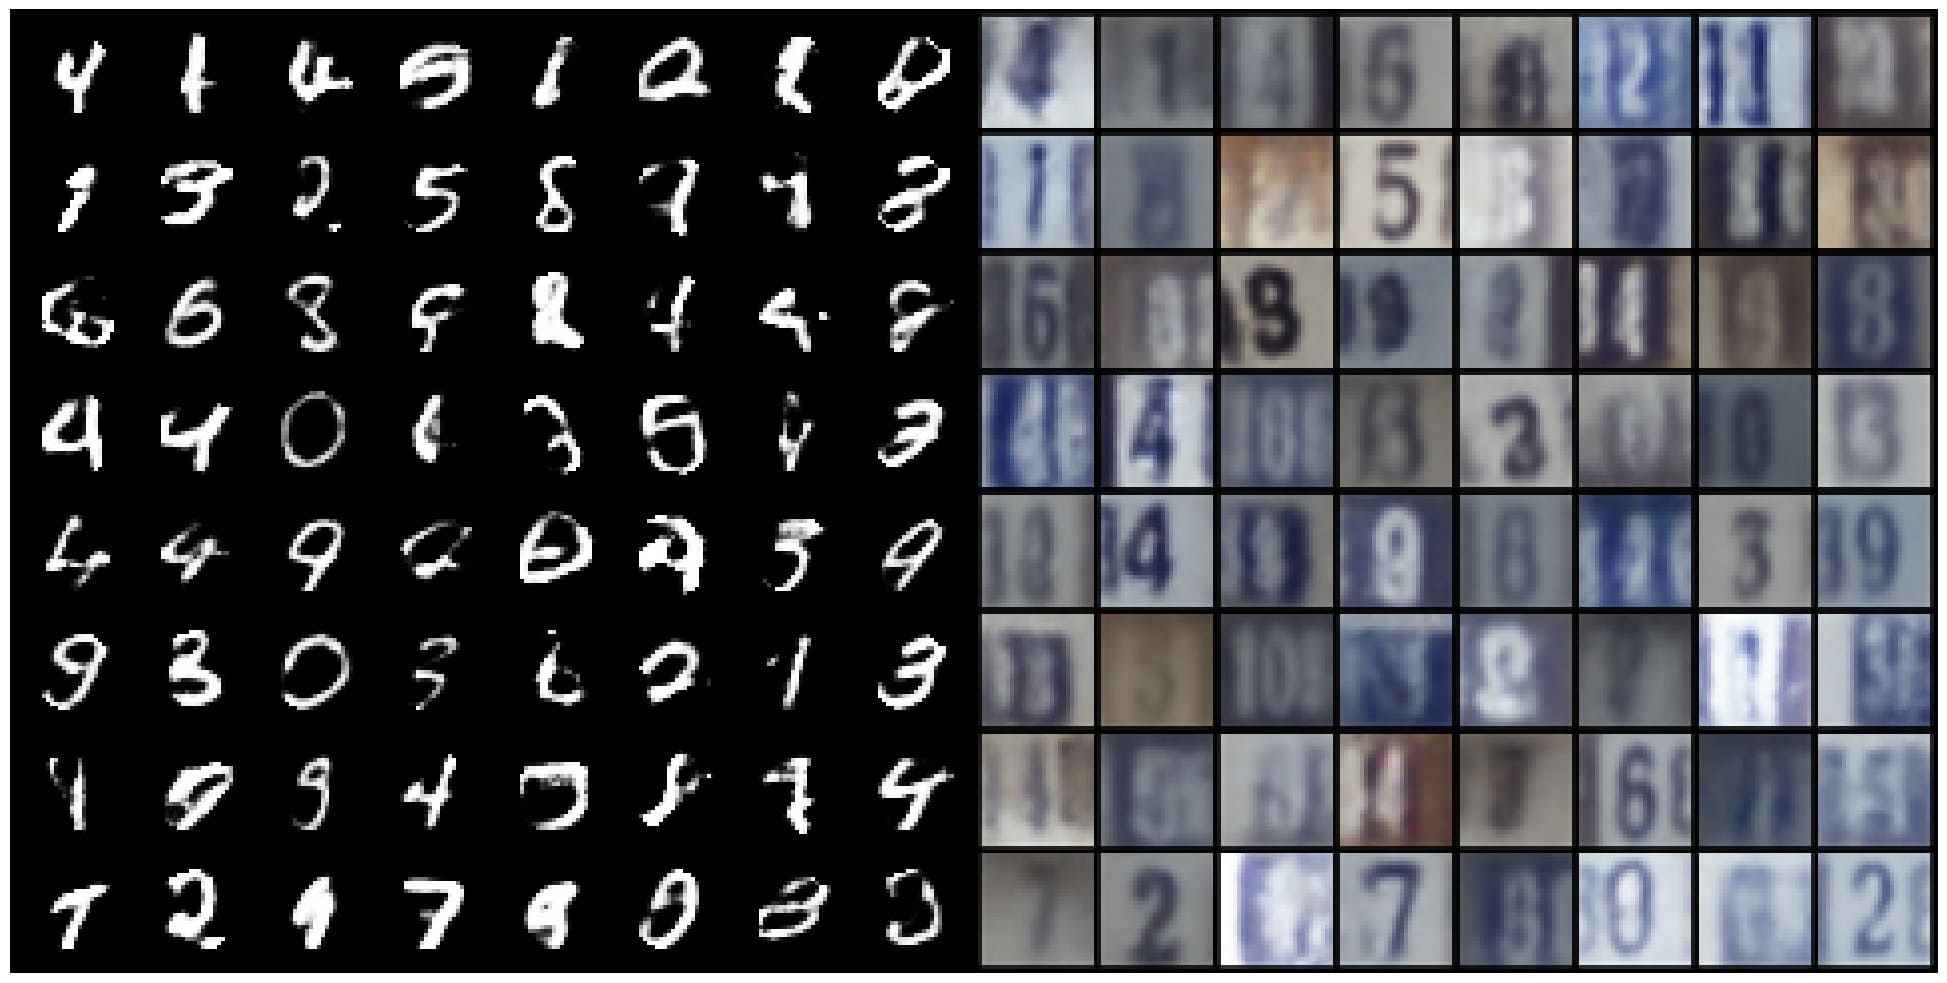
\includegraphics[width=\linewidth]{figures/datasets/ms/mvtcae_sampling_mnist_svhn}
         \caption*{\gls{MVTCAE}}
        
     \end{subfigure}
      \begin{subfigure}{0.40\textwidth}
         \centering
         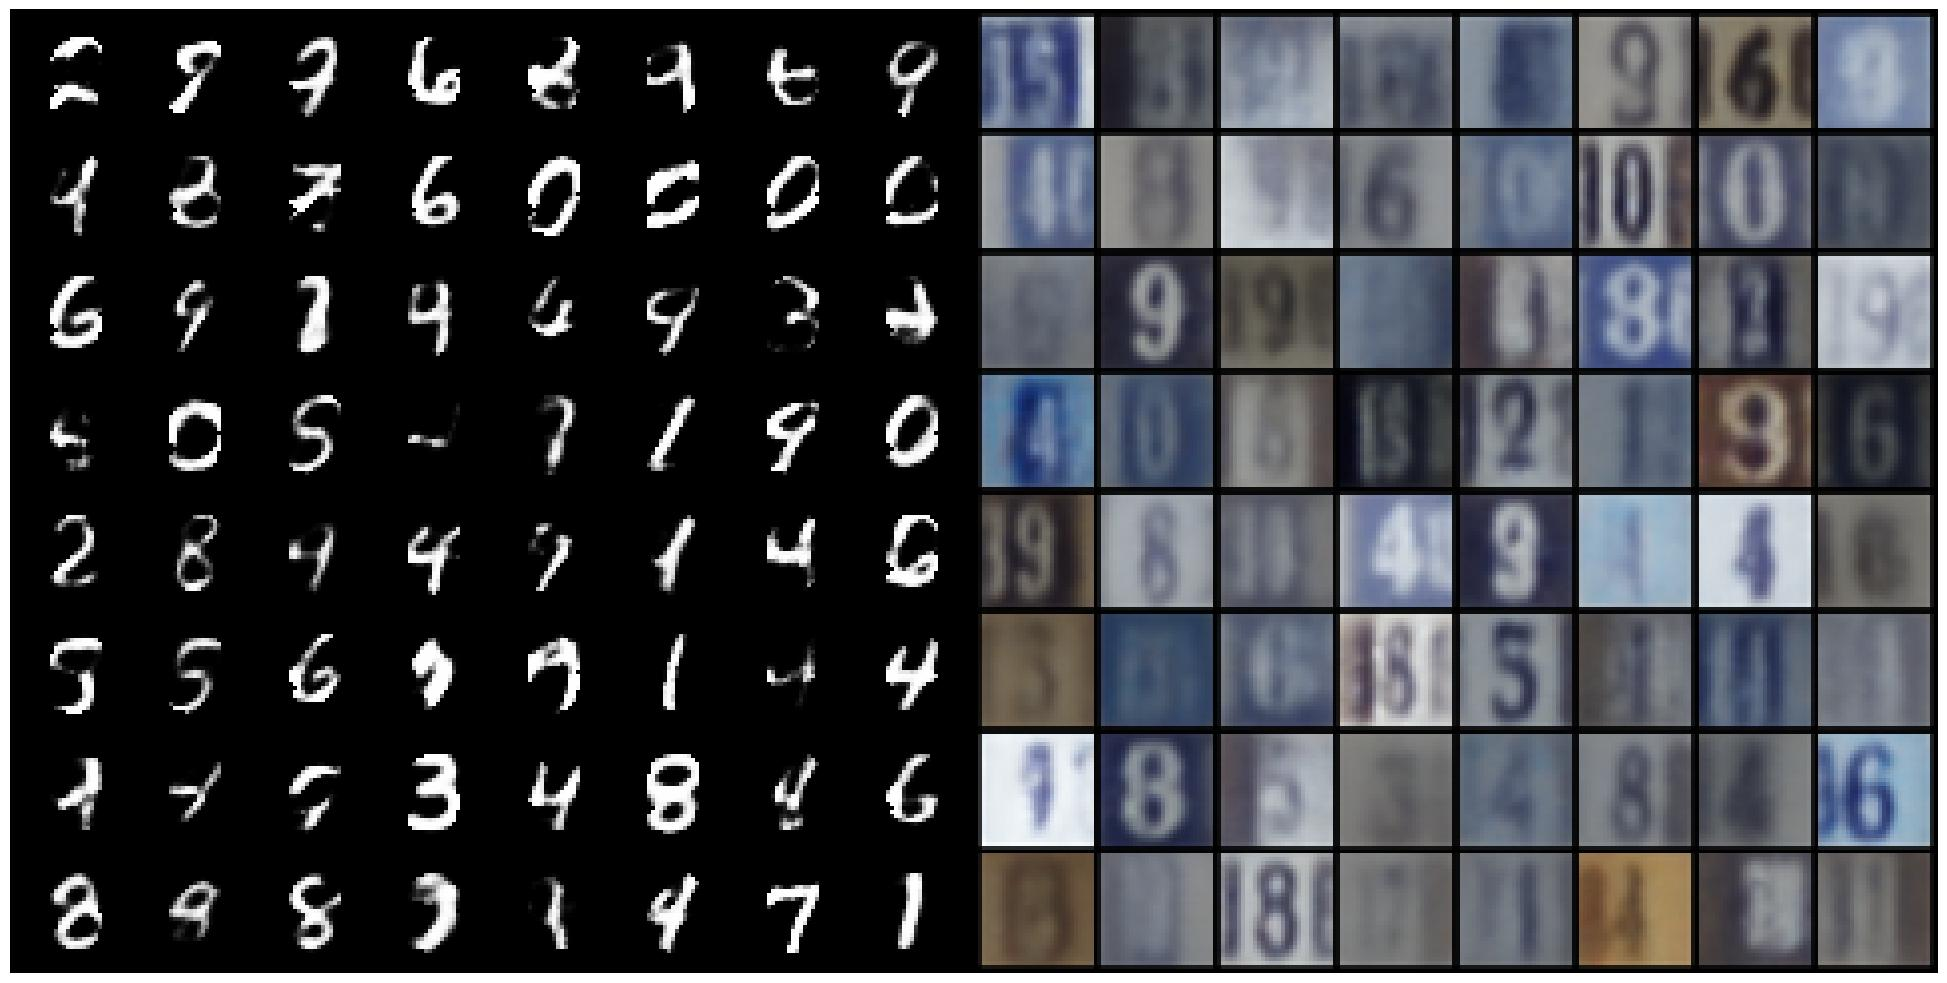
\includegraphics[page=1,width=\linewidth]{figures/datasets/ms/ms_mmvae+_sampling_mnist_svhn.jpg}
         \caption*{\gls{MMVAEplus}(K=10)  }
         
     \end{subfigure}
     
  \begin{subfigure}{0.40\textwidth}
         \centering
         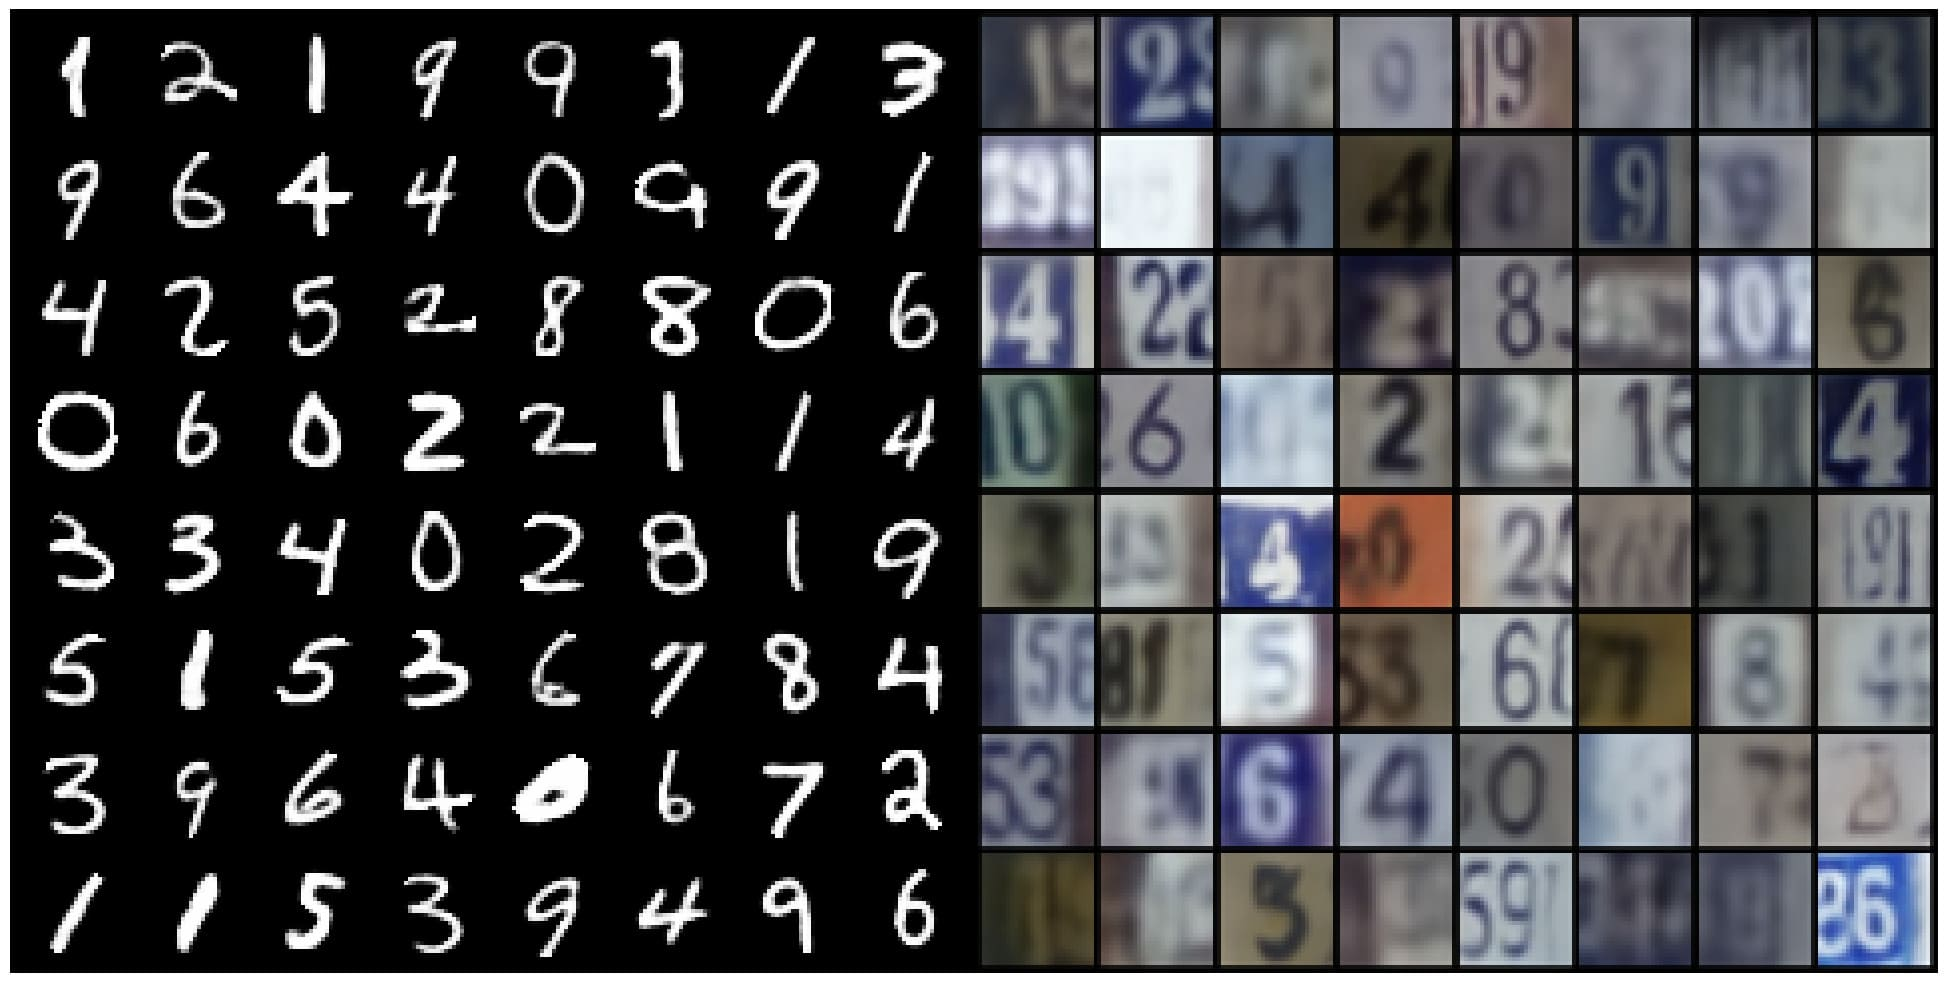
\includegraphics[page=1,width=\linewidth]{figures/datasets/ms/MLD_sampling_mnist_svhn}
         \caption*{\textbf{\gls{MLD} (ours) }  }
         
     \end{subfigure}
        \caption{Qualitative results for \textbf{\mnist-\svhn} joint generation.}
        \label{qualitative:ms_joint_detailed}
\end{figure}




\subsection{\mhd}



\begin{table}[H]
\centering
\caption{ Generative Coherence for \textbf{\mhd}. We report the detailed version of \Cref{coh:mhd} with standard deviation for 5 independent runs with different seeds.\newline}
\resizebox{\textwidth}{!}{\begin{tabular}{c|c|ccc|ccc|ccc}
\toprule
\multirow{2}{*}{ Models }  & \multirow{2}{*}{ Joint }
& \multicolumn{3}{c}{I (Image)}  & \multicolumn{3}{c}{T (Trajectory)}  & \multicolumn{3}{c}{S (Sound) } 
\\
\cmidrule{3-11}
    &&  T & S  & T,S  & I & S  & I,S & I & T & I,T \\
    \midrule
 \gls{MVAE}   &$37.77_{ \pm 3.32 }$ &
    
    $11.68_{\pm 0.35 }$ &
    $26.46 _{\pm 1.84 }$ & 
    $ 28.4_{\pm 1.47}$ & 
    
    $95.55_{\pm1.39}$  &
    $26.66 _{\pm 1.72 }$ &
     $96.58_{\pm1.06}$ &  
    
    $58.87_{\pm4.89}$ & 
    $10.39 _{\pm  0.42 }$  & 
    $58.16_{\pm5.24}$    \\

  \gls{MMVAE}   &    
    $34.78_{ \pm 0.83 }$ &
    
    $\textbf{99.7}_{\pm 0.03 }$ &
    $69.69 _{\pm 1.66}$ & 
    $ 84.74_{\pm 0.95}$ & 
    $\underline{99.3}_{ \pm 0.07 }$  &
    $85.46 _{\pm 1.57 }$  & 
    $92.39_{\pm0.95}$ &  
    
    $49.95_{\pm0.79}$ & 
    $50.14_{\pm  0.89 }$  & 
    $50.17_{\pm0.99}$   \\
    

    \gls{MOPOE}   &    $48.84_{ \pm 0.36 }$ &
    $\underline{99.64}_{\pm 0.08 }$ & $68.67 _{\pm 2.07 }$ & $ \underline{99.69}_{\pm 0.04}$ & 
    $99.28_{ \pm 0.08  }$  & $\underline{87.42}_{\pm  0.41 }$  & $99.35_{\pm0.04}$ &  
    $50.73_{\pm3.72}$ & $51.5 _{\pm  3.52 }$  & $56.97_{\pm6.34}$   \\

     \gls{NEXUS} &  $26.56_{ \pm 1.71 }$ &
    $94.58_{\pm 0.34 }$ & $\underline{83.1}_{\pm 0.74 }$ & $ 95.27_{\pm 0.52}$ & 
    $88.51_{ \pm 0.64  }$  & $76.82 _{\pm  3.63 }$  & $93.27_{\pm0.91}$ &  
    $70.06_{\pm2.83}$ & $75.84 _{\pm  2.53 }$  & $89.48_{\pm3.24}$ 
    \\

   
      \gls{MVTCAE} &  $42.28_{ \pm 1.12 }$ 
     &
    $99.54_{\pm 0.07 }$ & $72.05 _{\pm 0.95 }$ & $ 99.63_{\pm 0.05}$ & 
    $99.22_{ \pm 0.08  }$  & $72.03 _{\pm  0.48 }$  & $\underline{99.39}_{\pm0.02}$ &  
    $\underline{92.58}_{\pm0.47}$ & $\underline{93.07}_{\pm  0.36 }$  & $\underline{94.78}_{\pm0.25}$  \\

      \gls{MMVAEplus} &  $41.67_{ \pm 2.3 }$ 
     &
    $98.05_{\pm 0.19 }$ & $84.16_{\pm 	0.57 }$ & $ 91.88_{\pm }$ & 
    $97.47_{ \pm 0.89  }$  & $81.16_{\pm 2.24  }$  & $89.31_{\pm 1.54}$ &  
    $64.34_{\pm	4.46}$ & 
    $65.42_{\pm  5.42 }$  &
    $64.88_{\pm 4.93}$  \\

   \gls{MMVAEplus}(k=10) &  $42.60_{ \pm 2.5 }$ 
     &
    $99.44_{\pm 0.07 }$ & $\textbf{89.75} _{\pm 	0.75 }$ & $ 94.7_{\pm 0.72}$ & 
    $99.44_{ \pm 0.18  }$  
    & $\textbf{89.58}_{\pm 0.4  }$  & $95.01_{\pm0.30}$ &  
    $87.15_{\pm	2.81}$ & 
    $87.99_{\pm  2.55 }$  &
    $87.57_{\pm 2.09 }$  \\

    
    \midrule
 \gls{MLD} &  
 $\textbf{98.34}_{ \pm 0.22 }$
 &
    $99.45_{\pm 0.09 }$ &
    $\underline{88.91}_{\pm 0.54 }$ & 
    $ \textbf{99.88}_{\pm 0.04}$ & 
    
    $\textbf{99.58}_{ \pm 0.03  }$  & 
    $\underline{88.92} _{\pm  0.53 }$  & 
    $\textbf{99.91}_{\pm0.02}$ &  
    
    $\textbf{97.63}_{\pm0.14}$ & 
    $\textbf{97.7} _{\pm  0.34 }$ 
    & $\textbf{98.01}_{\pm 0.21}$  \\
    \bottomrule
   
\end{tabular}}
 \label{coh:mhd_detailed}

\end{table}





\begin{table}[h]
\centering
\caption{ Generative quality for \textbf{\mhd}. We report the detailed version of \Cref{qua:mhd} with standard deviation for 5 independent runs with different seeds.\newline}
\resizebox{\textwidth}{!}{\begin{tabular}{c|cccc|cccc|cccc}
\toprule
\multirow{2}{*}{ Models } & \multicolumn{4}{c}{I (Image)}  & \multicolumn{4}{c}{T (Trajectory)}  & \multicolumn{4}{c}{S (Sound) } 
\\
\cmidrule{2-13}
    & Joint & T & S  & T,S &  Joint &  I & S  & I,S & Joint  & I & T & I,T  \\
    \midrule
  \gls{MVAE}  & $\underline{94.9}_{ \pm7.37 }$   &  $93.73_{ \pm 5.44 }$ &
    $92.55_{ \pm 7.37 }$  &
    $91.08_{ \pm 10.24 }$  &
    


    $39.51_{ \pm 6.04 }$   &
    $20.42_{ \pm 4.42 }$ &
    $38.77_{ \pm 6.29 }$  &
    $19.25_{ \pm 4.26 }$  &
    
    $14.14_{ \pm 0.25 }$ &
  $\underline{14.13}_{ \pm 0.19 }$ &
    $14.08_{ \pm 0.24 }$  &
    $14.17_{ \pm 4.26 }$  
      

    \\
 \gls{MMVAE} & $224.01_{ \pm12.58 }$   &  $22.6_{ \pm 4.3 }$ &
    $789.12_{ \pm 12.58 }$  &
    $170.41_{ \pm 8.06 }$  &
    
    $16.52_{ \pm1.17 }$   & 
    $\textbf{0.5}_{ \pm 0.05 }$ &
    $30.39_{ \pm 1.38 }$  &
    $6.07_{ \pm 0.37 }$  &
    


 $22.8_{ \pm0.39 }$    &
    $22.61_{ \pm 0.75 }$ &
    $23.72_{ \pm 0.86 }$  &
    $23.01_{ \pm 0.67 }$  
   

\\
  \gls{MOPOE} &  $147.81_{ \pm10.37 }$   &  $16.29_{ \pm 0.85 }$ &
    $838.38_{ \pm 10.84 }$  &
    $15.89_{ \pm 1.96 }$  &
   
 $\underline{13.92}_{ \pm0.96 }$   & 
$\underline{0.52}_{ \pm 0.12 }$ &
    $33.38_{ \pm 1.14 }$  &
    $\textbf{0.53}_{ \pm 0.1 }$  &
   
       $18.53_{ \pm0.27 }$&
    $24.11_{ \pm0.4 }$ &
    $24.1_{ \pm 0.41 }$  &
    $23.93_{ \pm 0.87 }$  

    \\
   \gls{NEXUS} &  $281.76_{ \pm12.69 }$   &      $116.65_{ \pm 9.99 }$ &
    $282.34_{ \pm 12.69 }$  &
    $117.24_{ \pm 8.53 }$  &
    
      $18.59_{ \pm2.16 }$   &
    $6.67_{ \pm 0.23 }$ &
    $33.01_{ \pm 3.41 }$  &
    $7.54_{ \pm 0.29 }$  &
  
       $\underline{13.99}_{ \pm0.9}$   &
    $19.52_{ \pm 0.14 }$ &
    $18.71_{ \pm 0.24 }$  &
    $16.3_{ \pm 0.59 }$  
 

    \\


   \gls{MVTCAE} &    $121.85_{ \pm 3.44 }$   &   $\underline{5.34}_{ \pm 0.33 }$ &
    $\underline{54.57}_{ \pm 7.79 }$  &
    $\underline{3.16}_{ \pm 0.26 }$  &
 

        $19.49_{ \pm 0.67}$   & 
    $0.62_{ \pm 0.1}$ &
    $\underline{13.65}_{ \pm 1.24 }$  &
    $0.75_{ \pm 0.13 }$  &


        $15.88_{ \pm 0.19}$   &
        $14.22_{ \pm 0.27}$ &
    $\underline{14.02}_{ \pm 0.14 }$  &
    $\underline{13.96}_{ \pm 0.28}$
    \\

    
   \gls{MMVAEplus} &    
   
   $97.19_{ \pm 12.37 }$   &  
   $2.80_{ \pm 0.42 }$ &
    $128.56_{ \pm 4.47 }$  &
    $ 114.3_{ \pm 11.4 }$  &
 

        $22.37_{ \pm 1.87}$   & 
    $1.21_{ \pm 0.22}$ &
    $21.74_{ \pm 3.49 }$  &
    $15.2_{ \pm 1.15 }$  &


        $16.12_{ \pm 0.40}$   &
        $17.31_{ \pm 0.62}$ &
    $17.92_{ \pm 0.19 }$  &
    $17.56_{ \pm 0.48}$
    
    \\

     \gls{MMVAEplus}(K=10) &    
   
   $85.98_{ \pm 1.25 }$   &  
   $1.83_{ \pm 0.26 }$ &
    $70.72_{ \pm 1.76 }$  &
    $62.43_{ \pm 3.4  }$  &
 

        $21.10_{ \pm 1.25}$   & 
    $1.38_{ \pm 0.34}$ &
    $8.52_{ \pm 0.79 }$  &
    $7.22_{ \pm 1.6 }$  &


   $14.58_{ \pm 0.47 }$   &  
   $14.33_{ \pm 0.51 }$ &
    $14.34_{ \pm 0.42 }$  &
    $14.32_{ \pm 0.6 }$  
    
    \\
    \midrule
      
   \textbf{\gls{MLD} (ours) }&     $\textbf{7.98}_{ \pm 1.41 }$ & $\textbf{1.7}_{ \pm 0.14 }$ &
    $\textbf{4.54}_{ \pm 0.45 }$ & 
    $\textbf{1.84}_{ \pm 0.27 }$  &
 
      $\textbf{3.18}_{ \pm 0.18 }$ 
      & $0.83_{ \pm 0.03 }$ 
     & $\textbf{2.07}_{ \pm 0.26 }$ 
       & $\underline{0.6}_{ \pm 0.05}$ 
      

 & $ \textbf{2.39}_{ \pm 0.1 } $
        & $\textbf{2.31}_{ \pm 0.07 }$ 
     & $\textbf{2.33}_{ \pm 0.11 }$ 
       & $\textbf{	2.29}_{ \pm 0.06 }$ 
      
       \\

    \bottomrule
   
\end{tabular}}


 \label{qua:mhd_detailed}

\end{table}








\begin{figure}[h]
     \centering
       \centering
     \begin{subfigure}{0.25\textwidth}
         \centering
         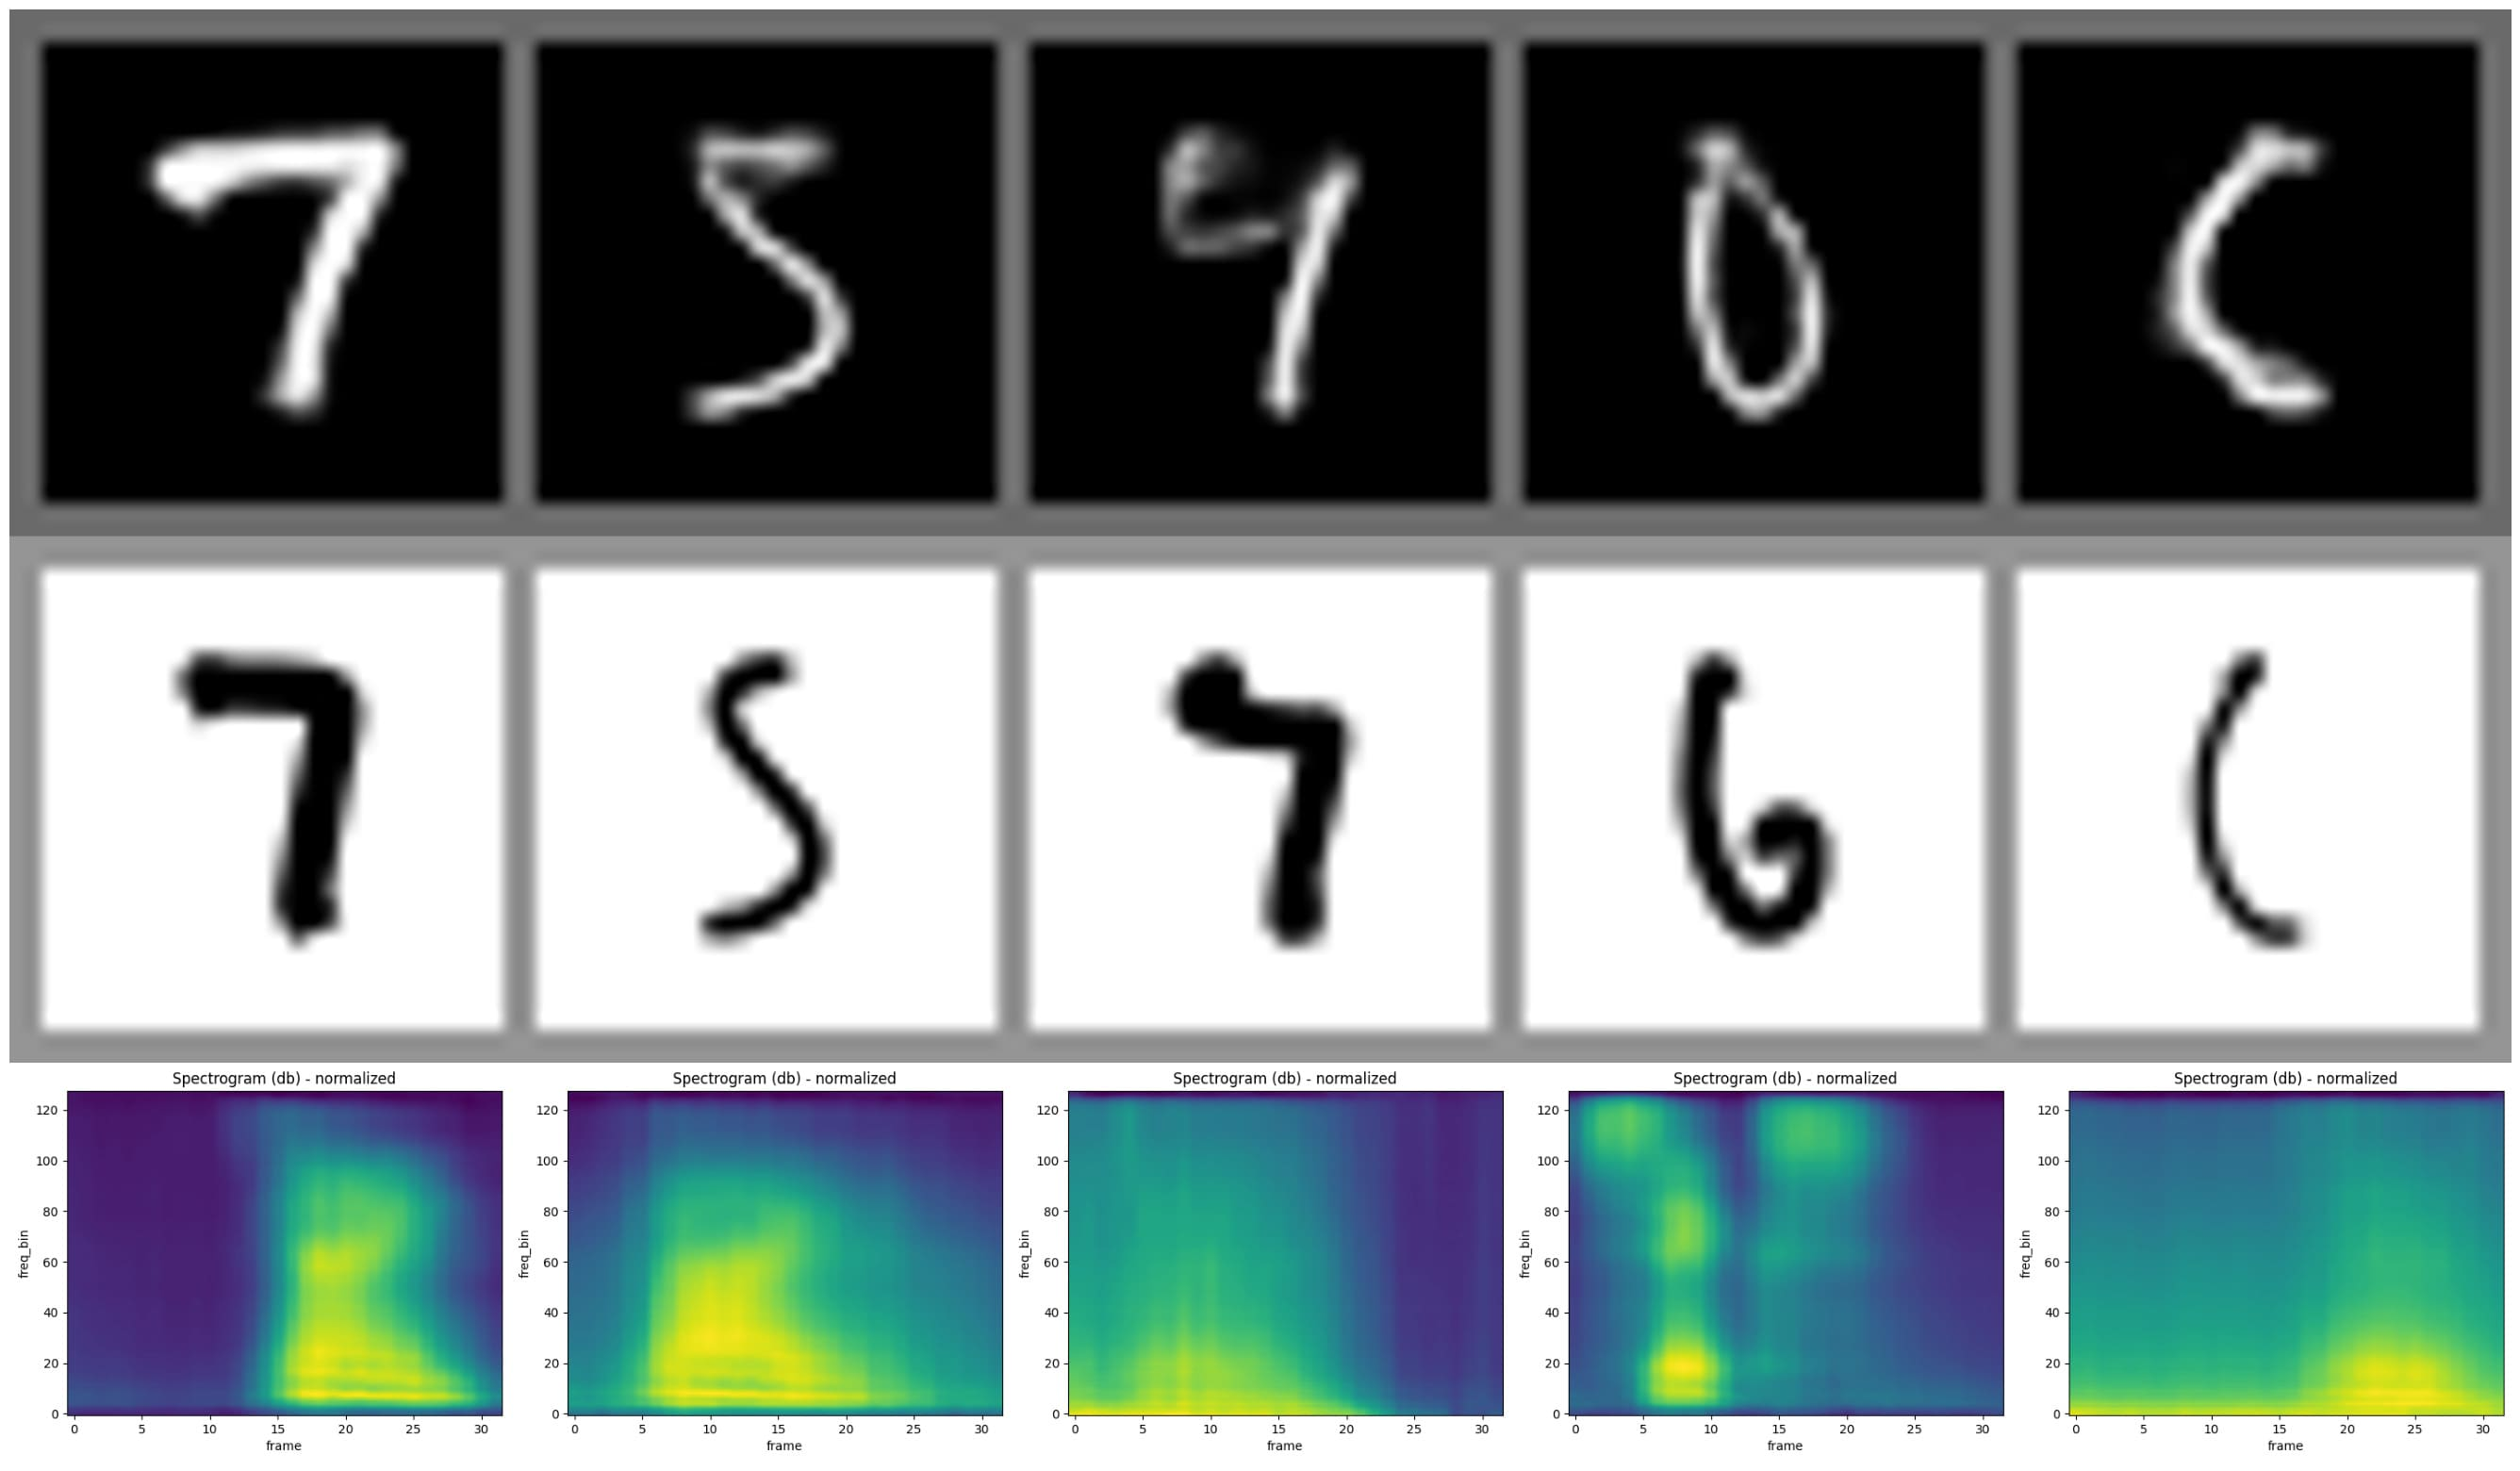
\includegraphics[width=\linewidth]{figures/datasets/mhd/mvae_sampling_mhd}
  \caption*{\gls{MVAE}}
     \end{subfigure}
     \begin{subfigure}{0.25\textwidth}
         \centering
         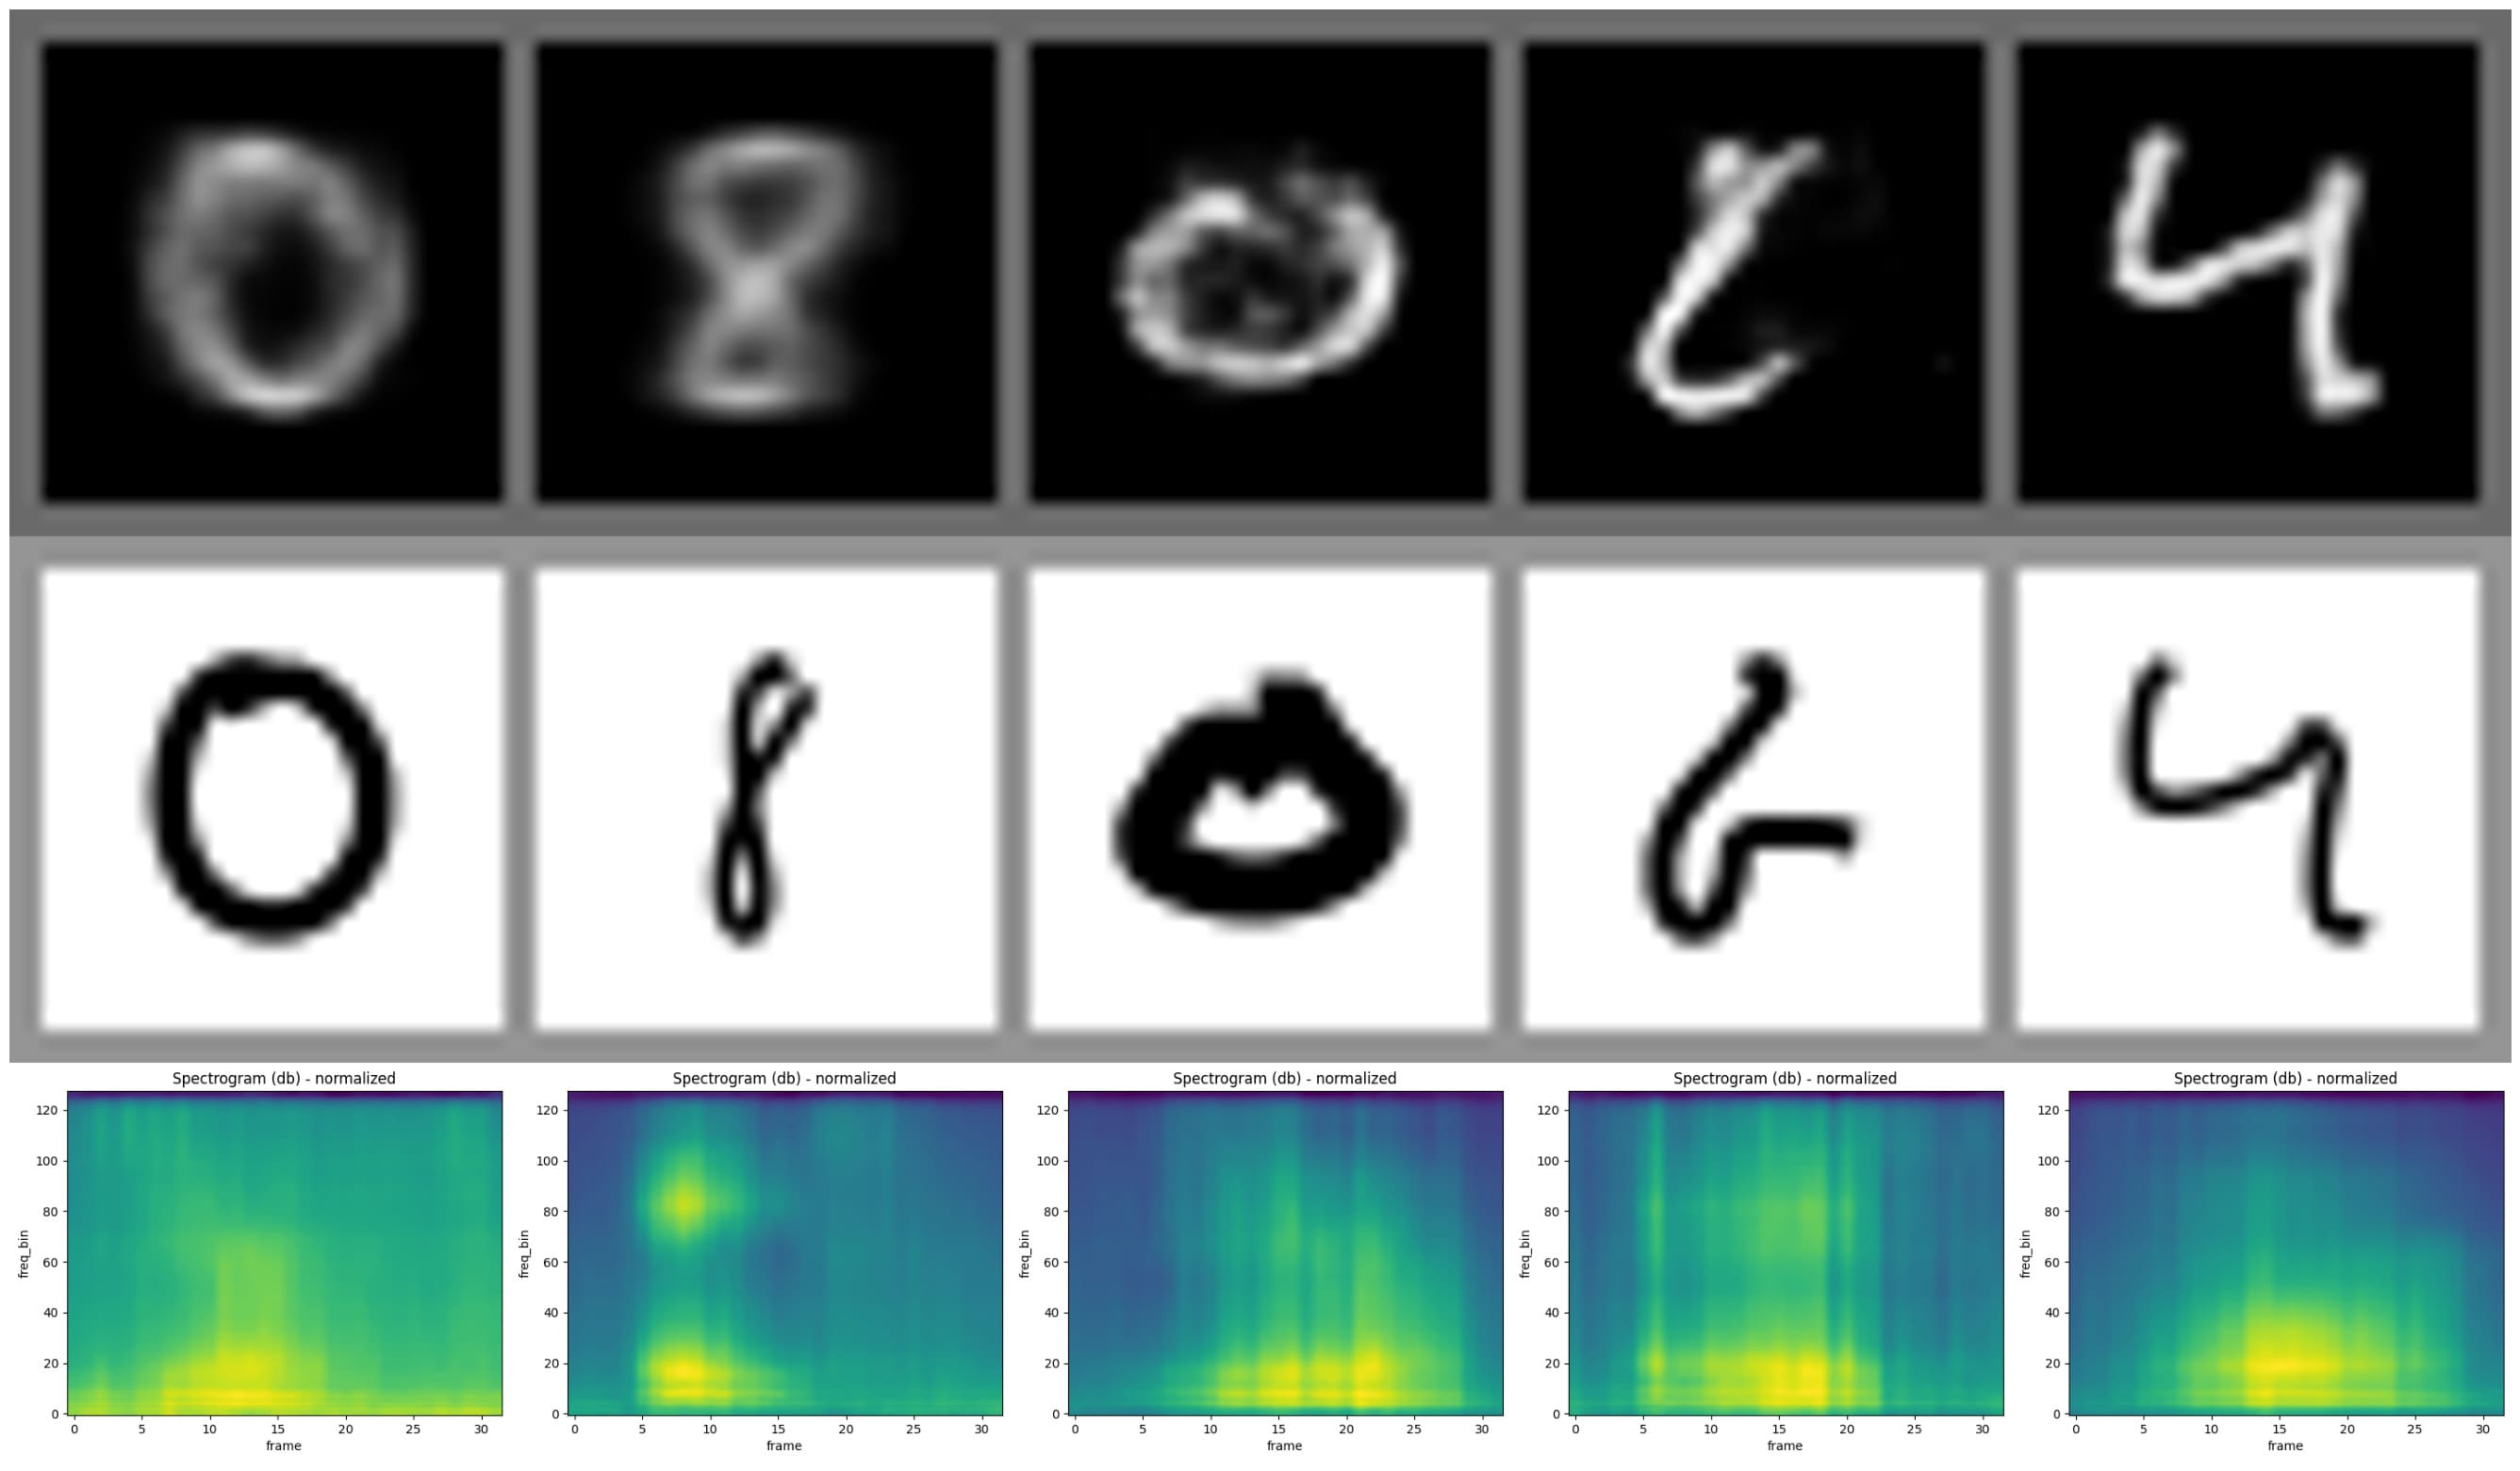
\includegraphics[width=\linewidth]{figures/datasets/mhd/mmvae_sampling_mhd}
   \caption*{\gls{MMVAE}}
     \end{subfigure}
       \begin{subfigure}{0.25\textwidth}
         \centering
         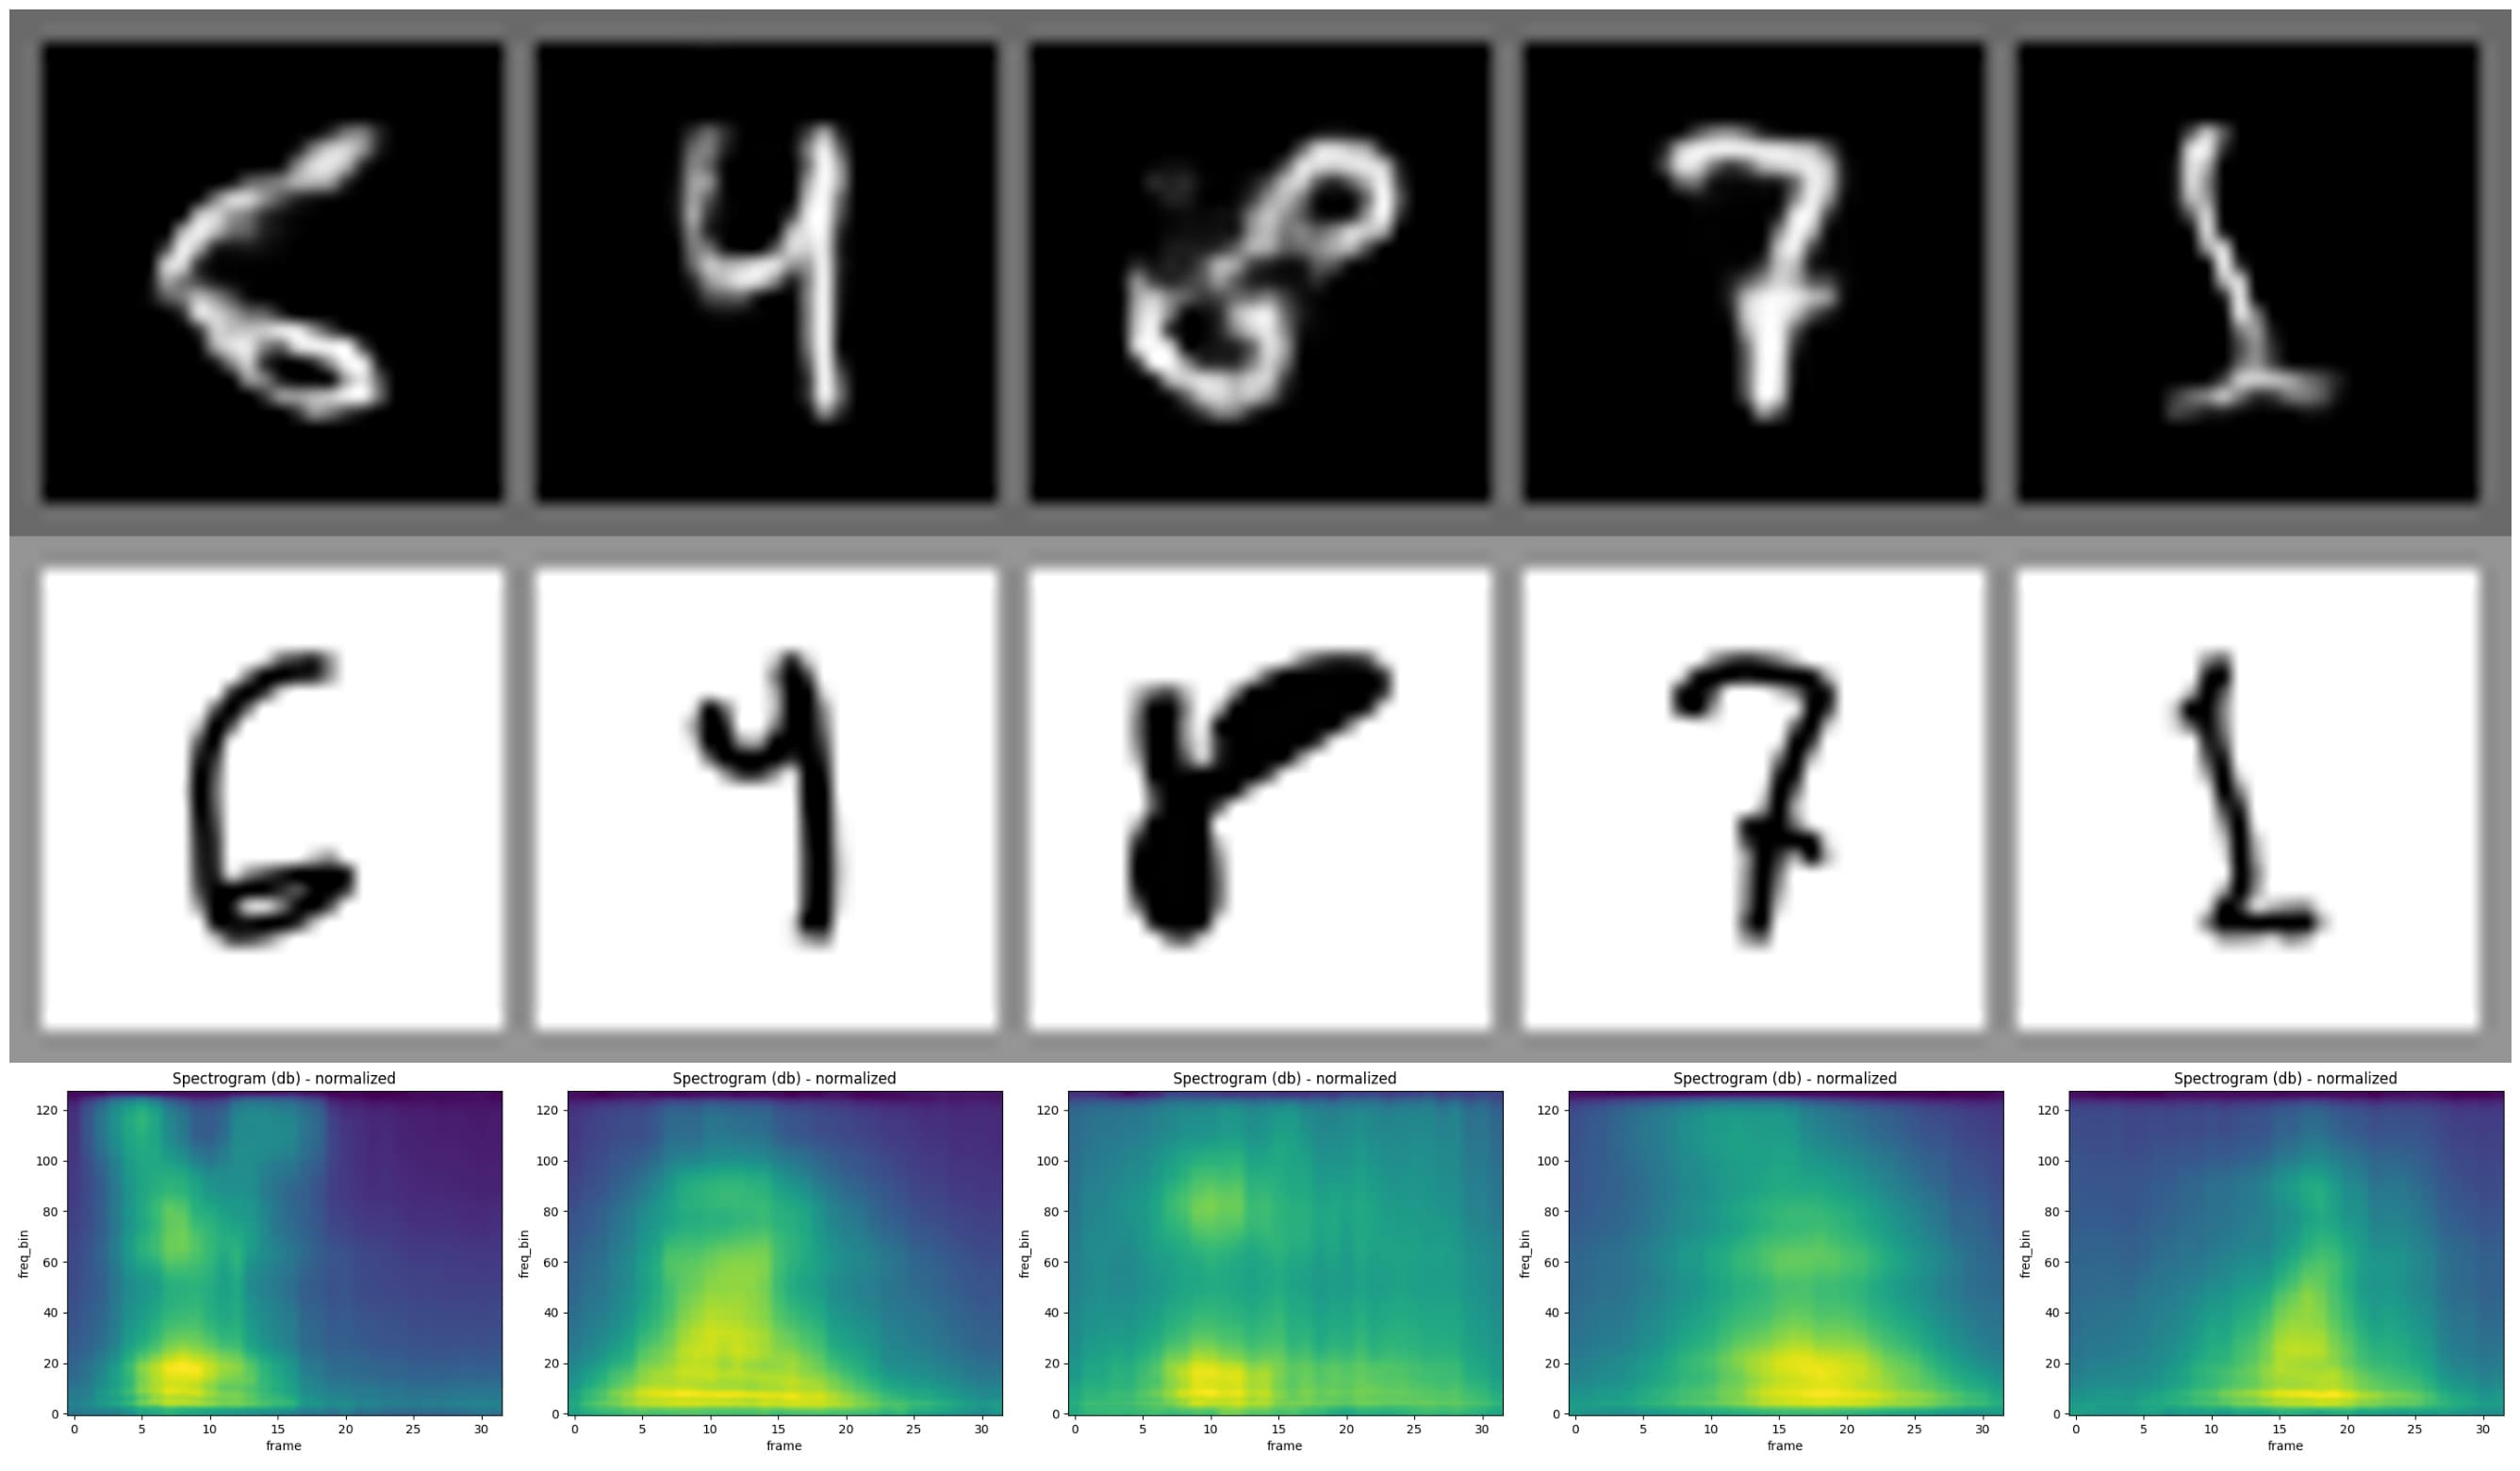
\includegraphics[width=\linewidth]{figures/datasets/mhd/mopoe_sampling_mhd}
         \caption*{\gls{MOPOE}}
     \end{subfigure}
     
      \begin{subfigure}{0.25\textwidth}
         \centering
         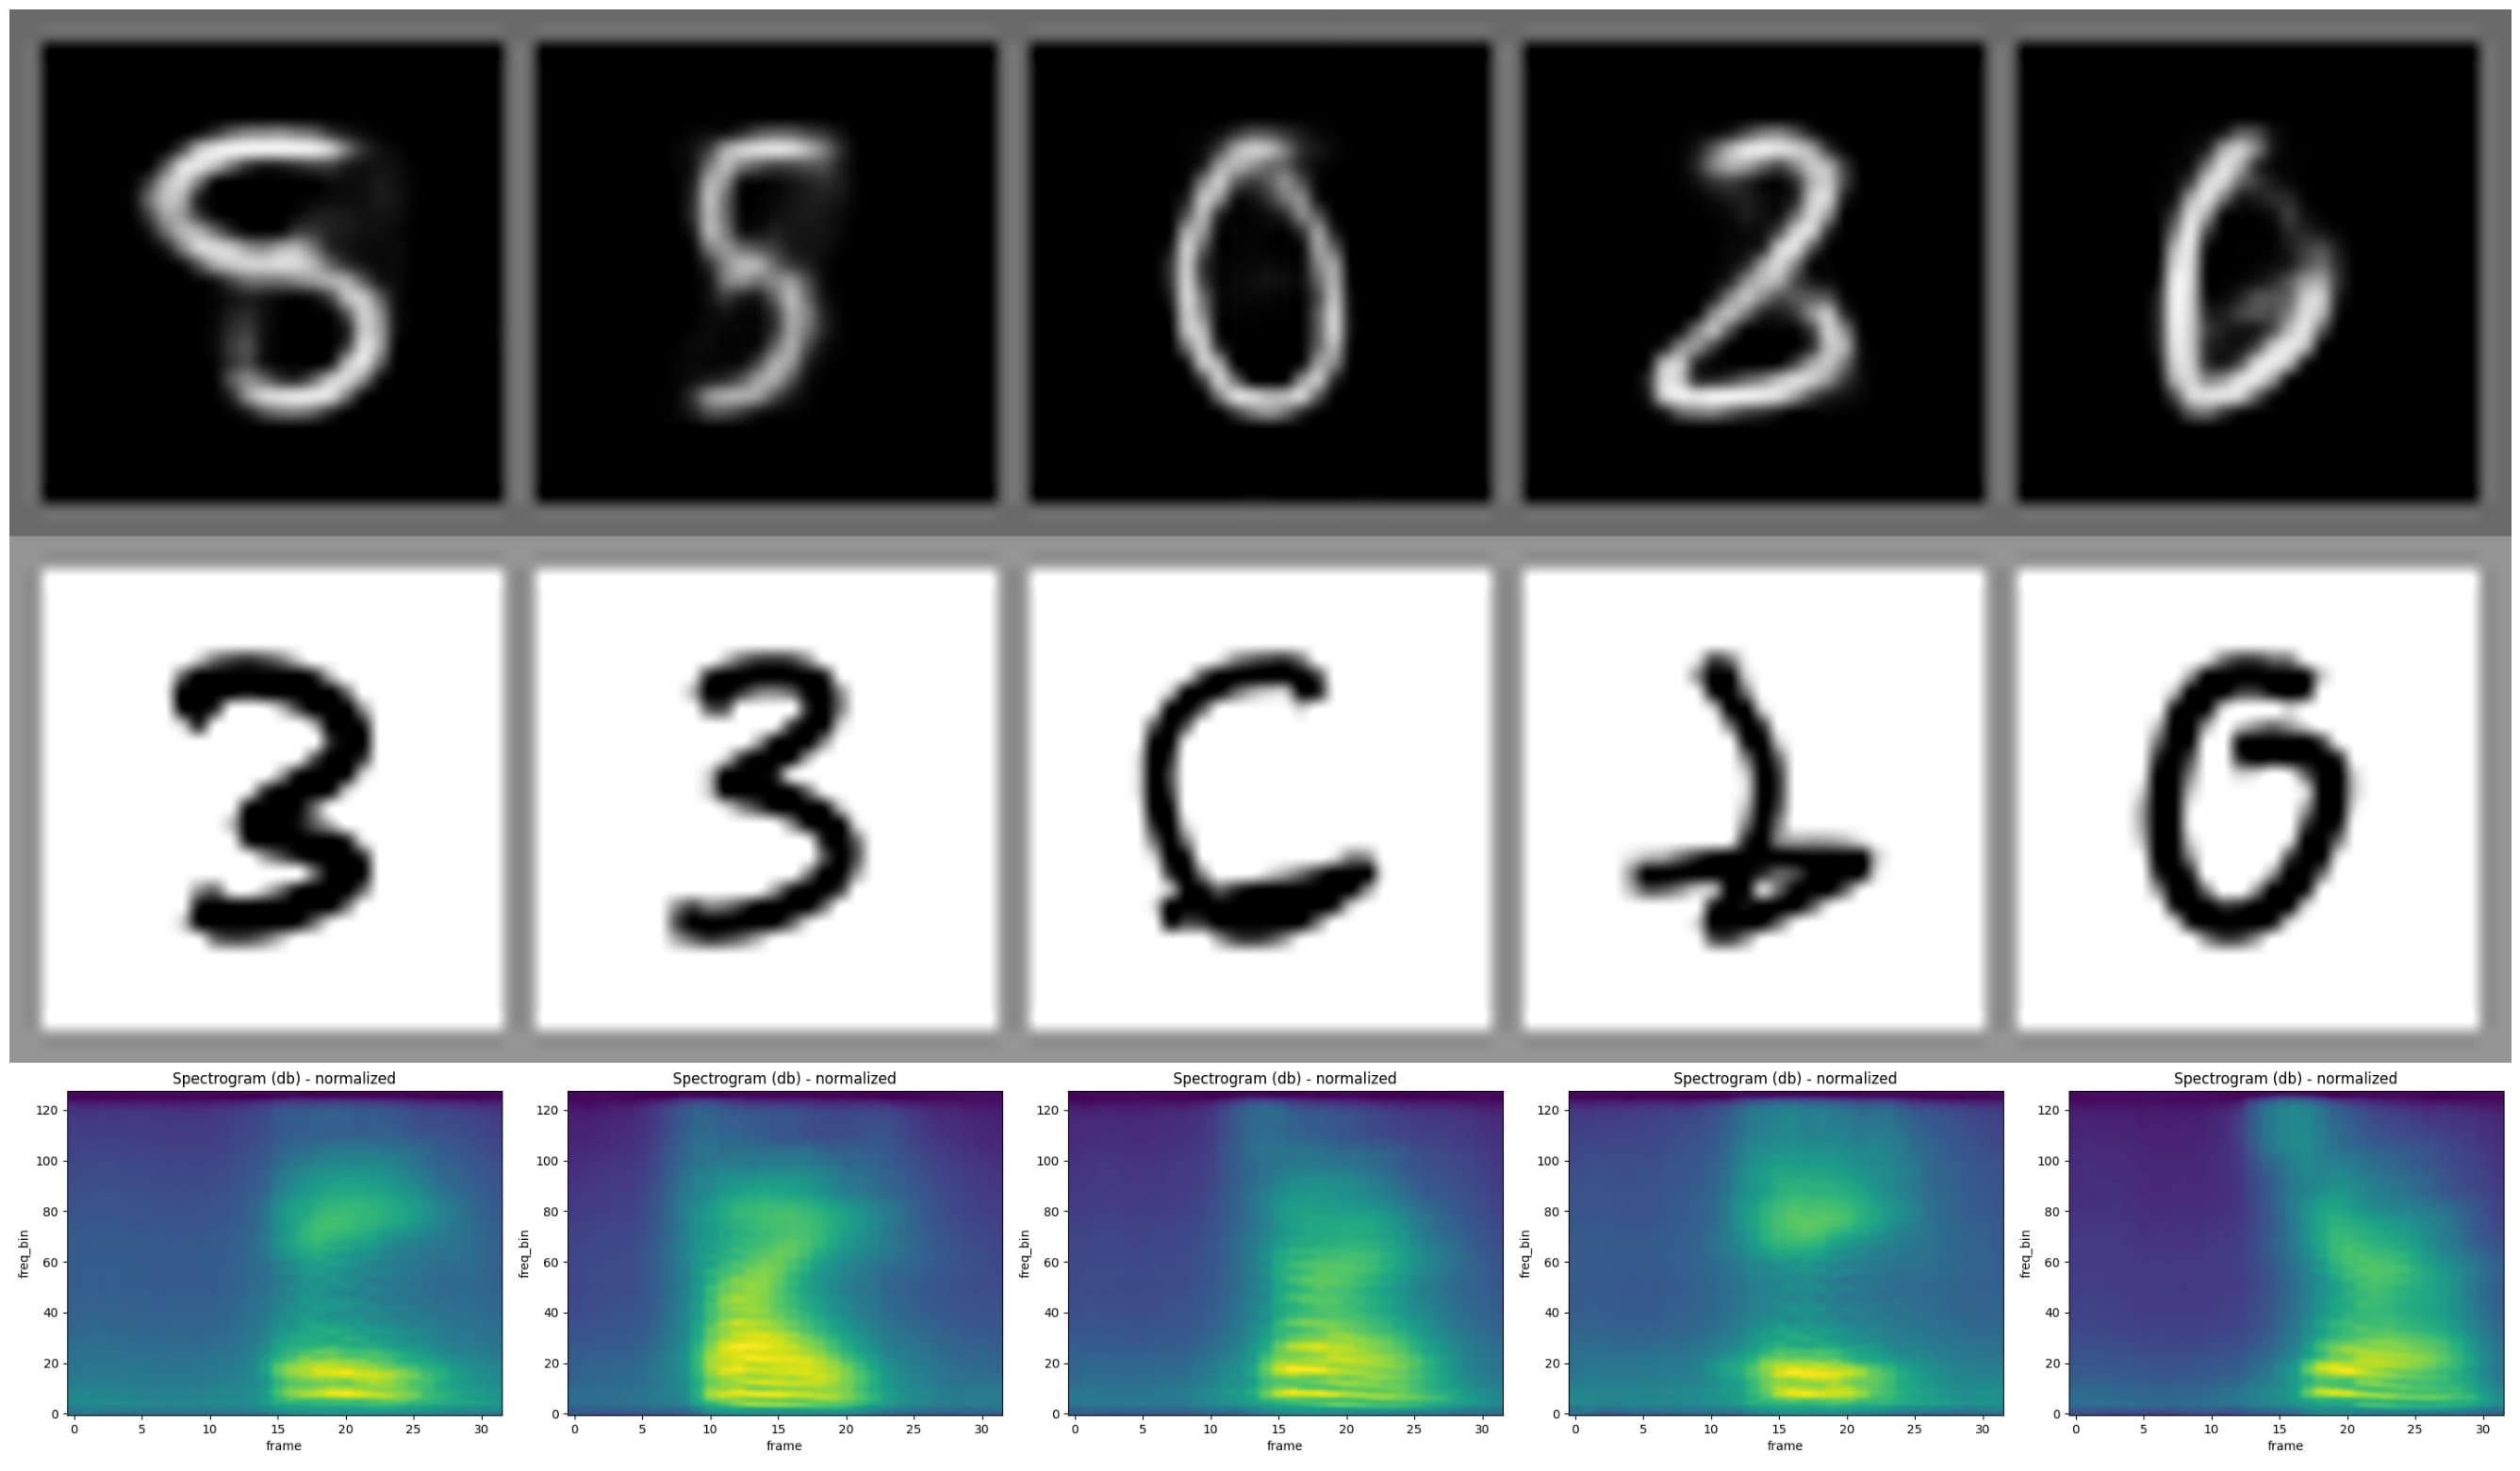
\includegraphics[width=\linewidth]{figures/datasets/mhd/nexus_sampling_mhd}
         \caption*{\gls{NEXUS}}
     \end{subfigure}
  \begin{subfigure}{0.25\textwidth}
         \centering
         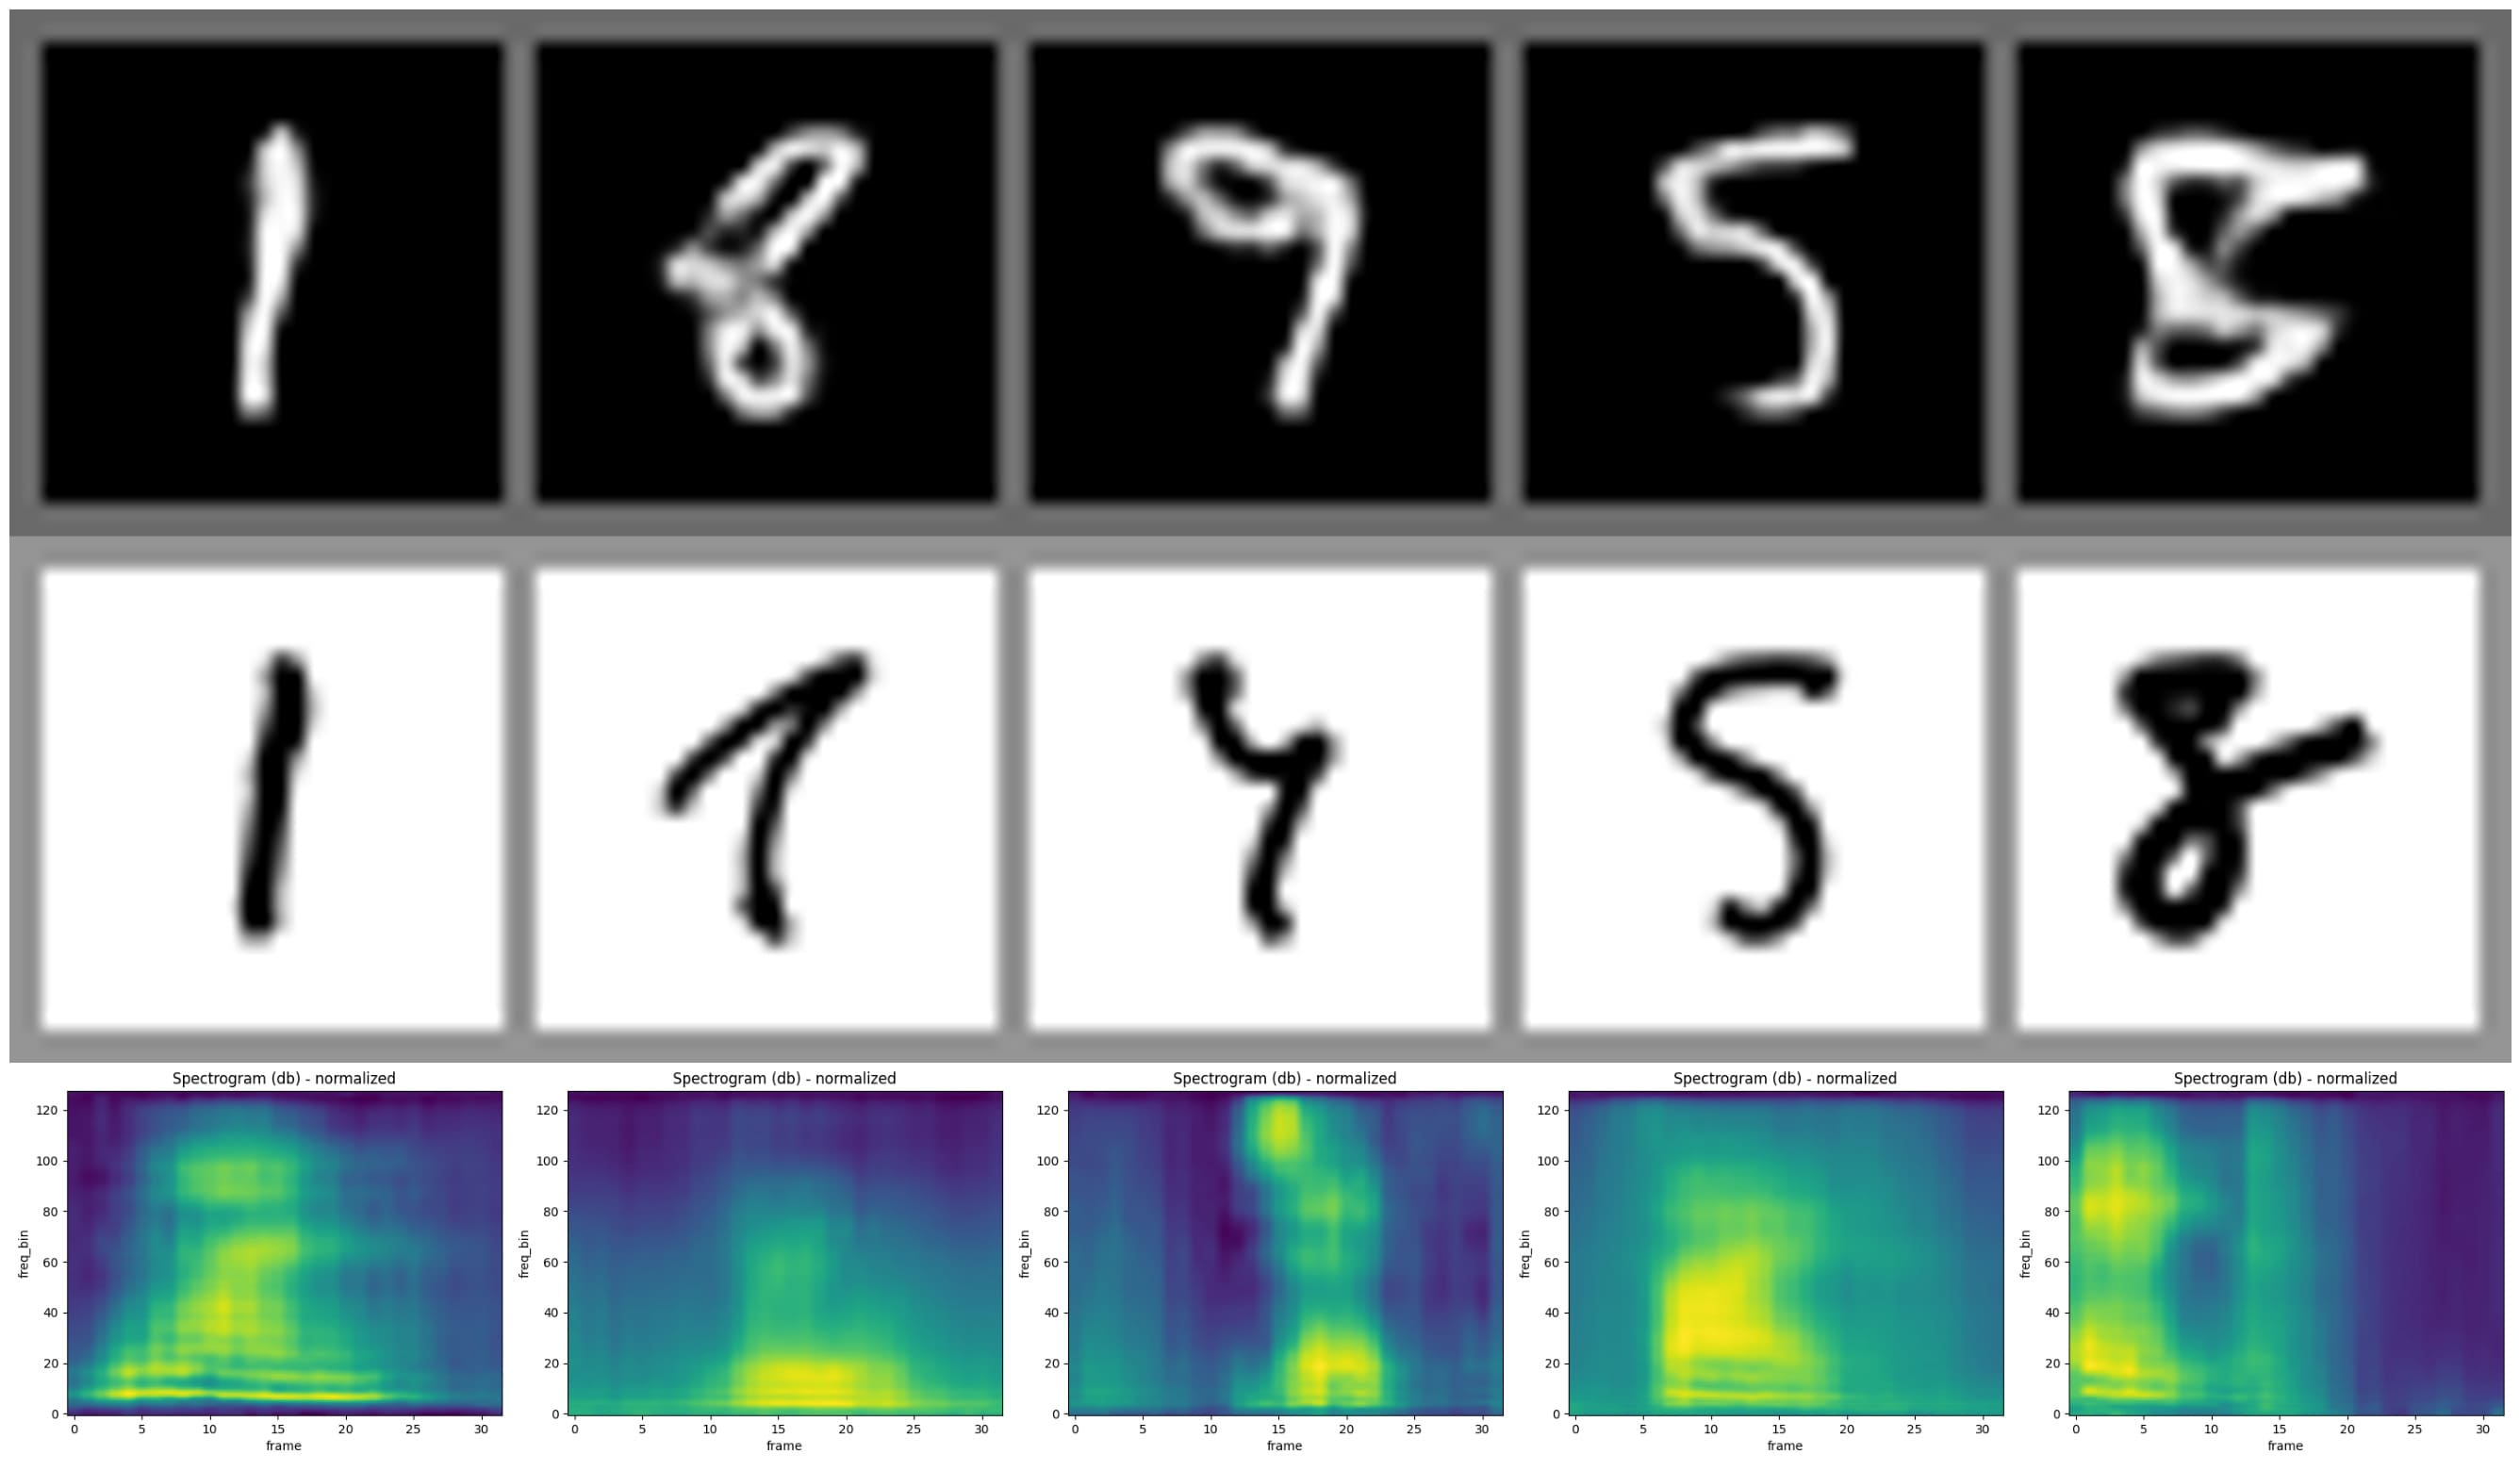
\includegraphics[width=\linewidth]{figures/datasets/mhd/tcmvae_sampling_mhd}
         \caption*{\gls{MVTCAE}}
     
     \end{subfigure}
    \begin{subfigure}{0.25\textwidth}
         \centering
         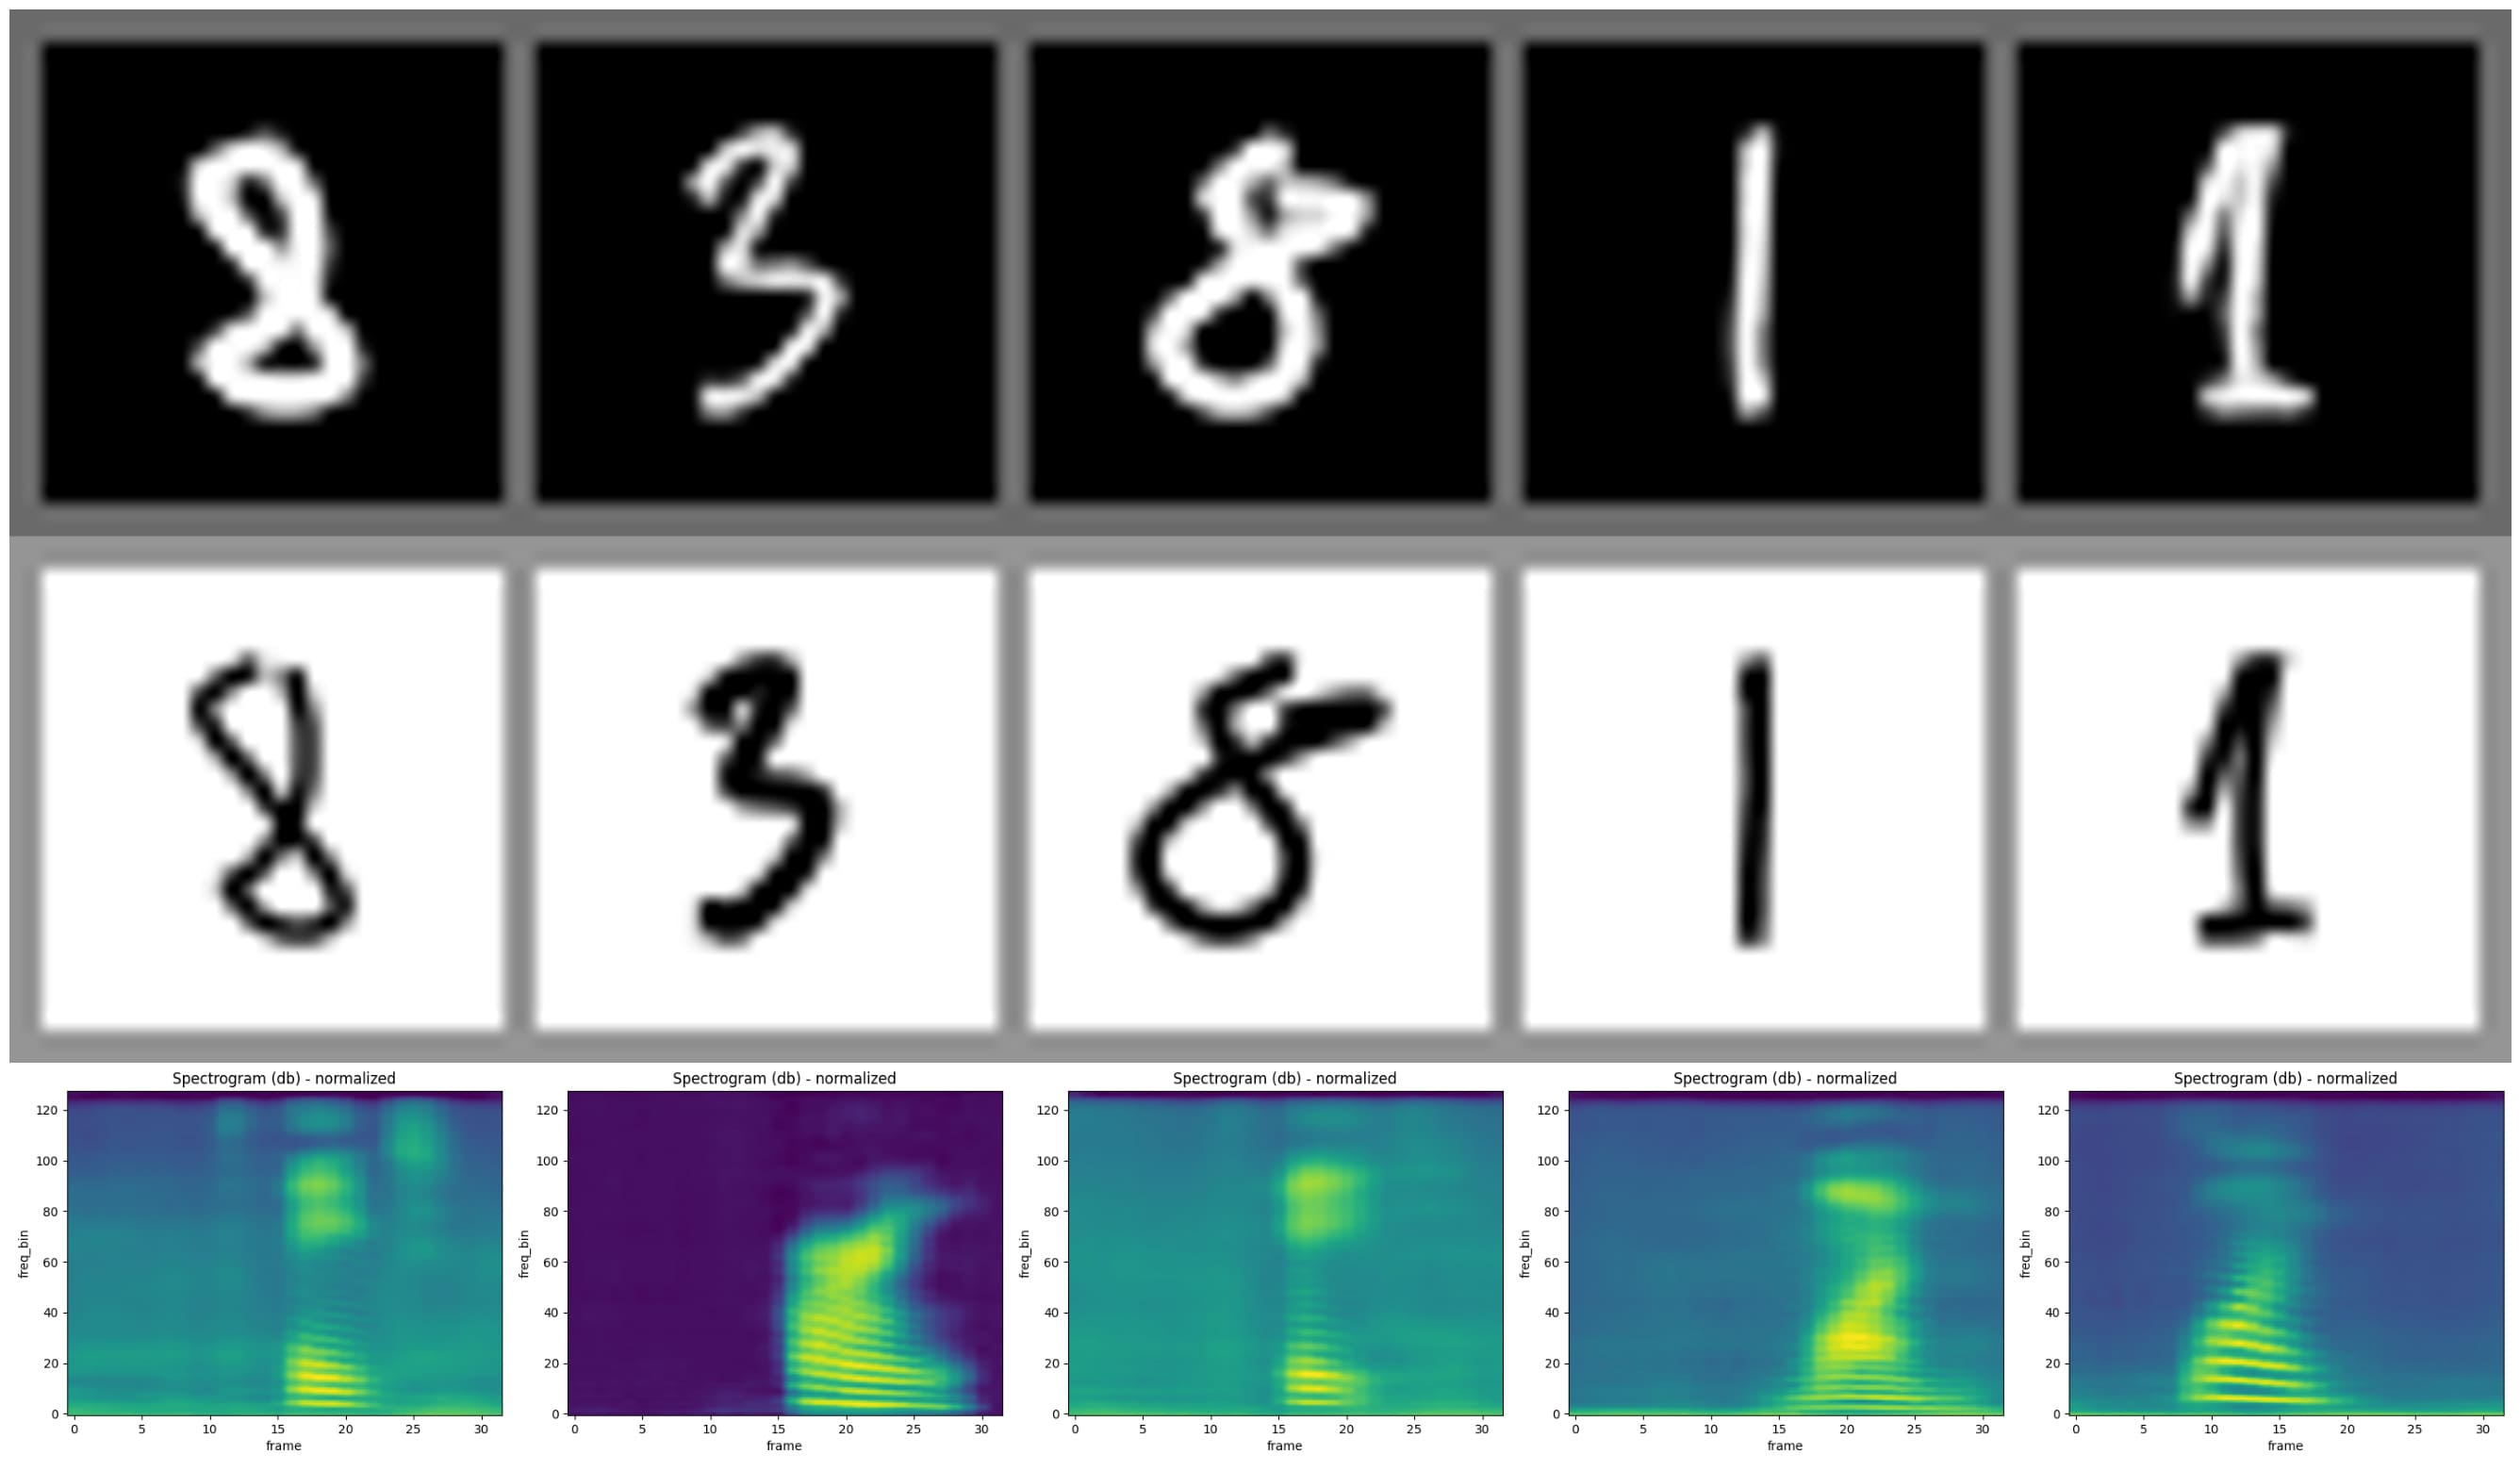
\includegraphics[page=1,width=\linewidth]{figures/datasets/mhd/MLD_inpaint_sampling_mhd}
         \caption*{\gls{MLD Inpaint} }
     \end{subfigure}
     
  \begin{subfigure}{0.25\textwidth}
         \centering
         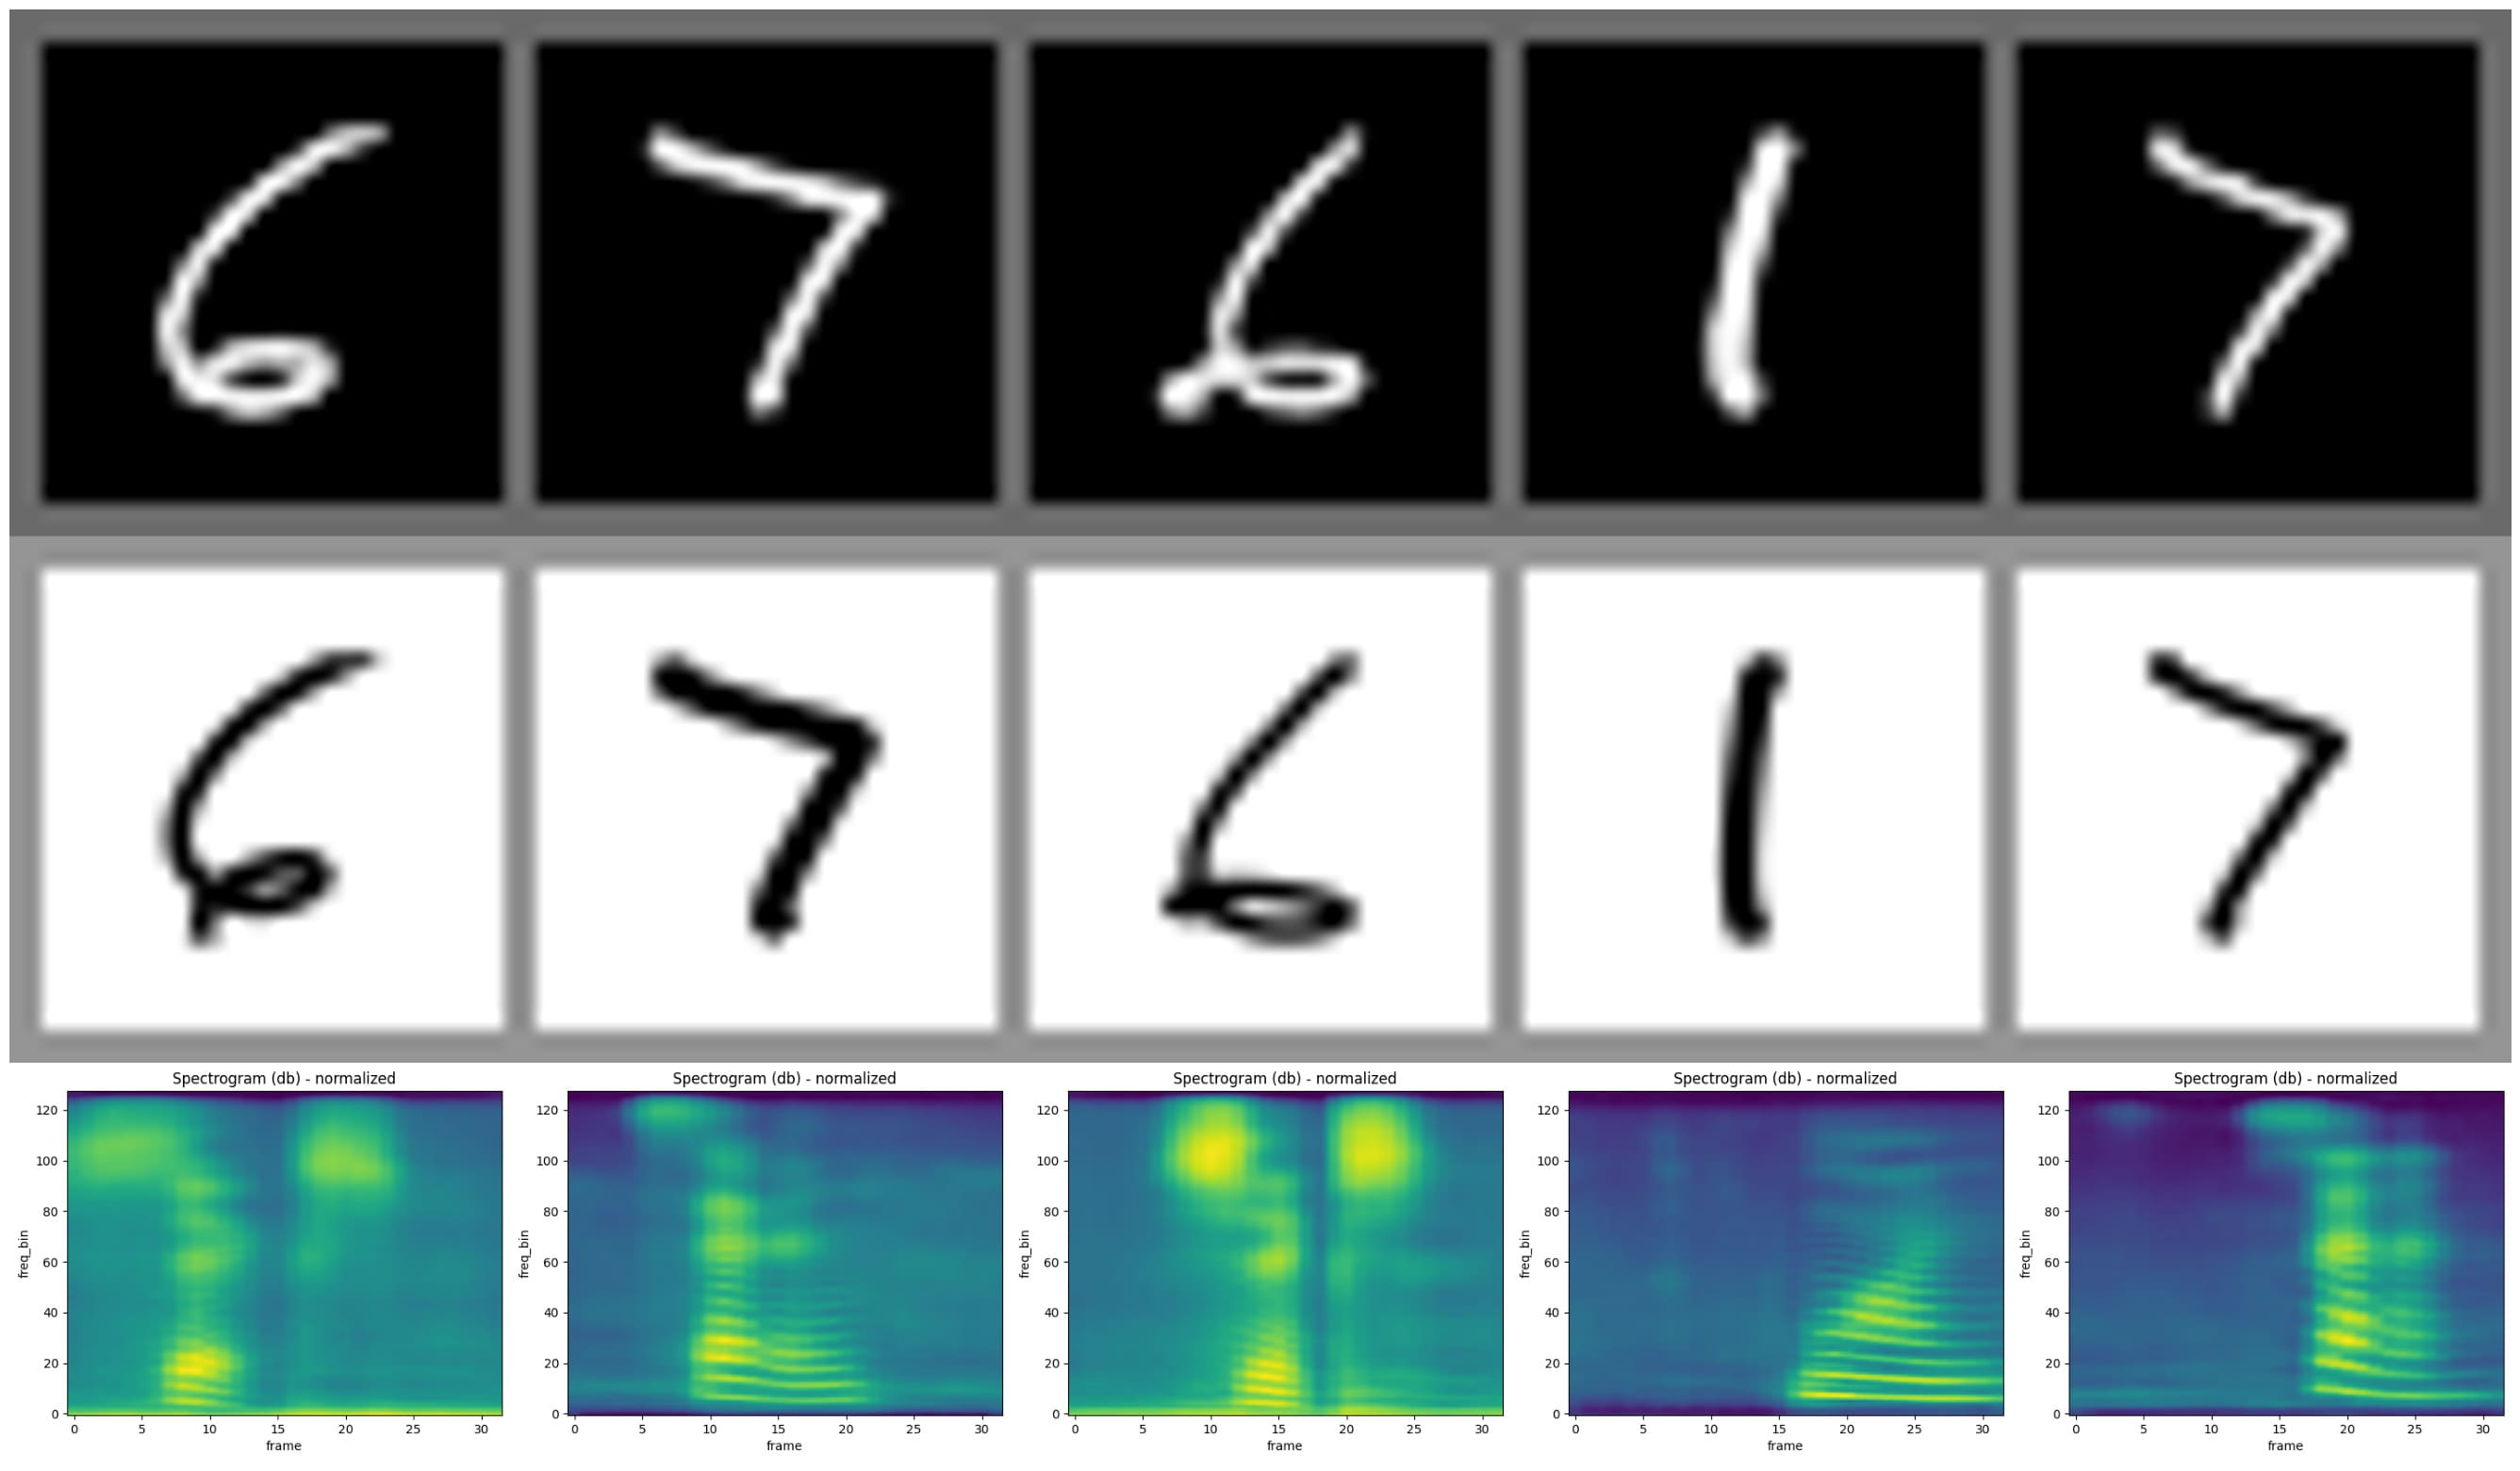
\includegraphics[page=1,width=\linewidth]{figures/datasets/mhd/MLD_uni_sampling_mhd}
         \caption*{\gls{MLD Uni} }
     \end{subfigure}
  \begin{subfigure}{0.25\textwidth}
         \centering
         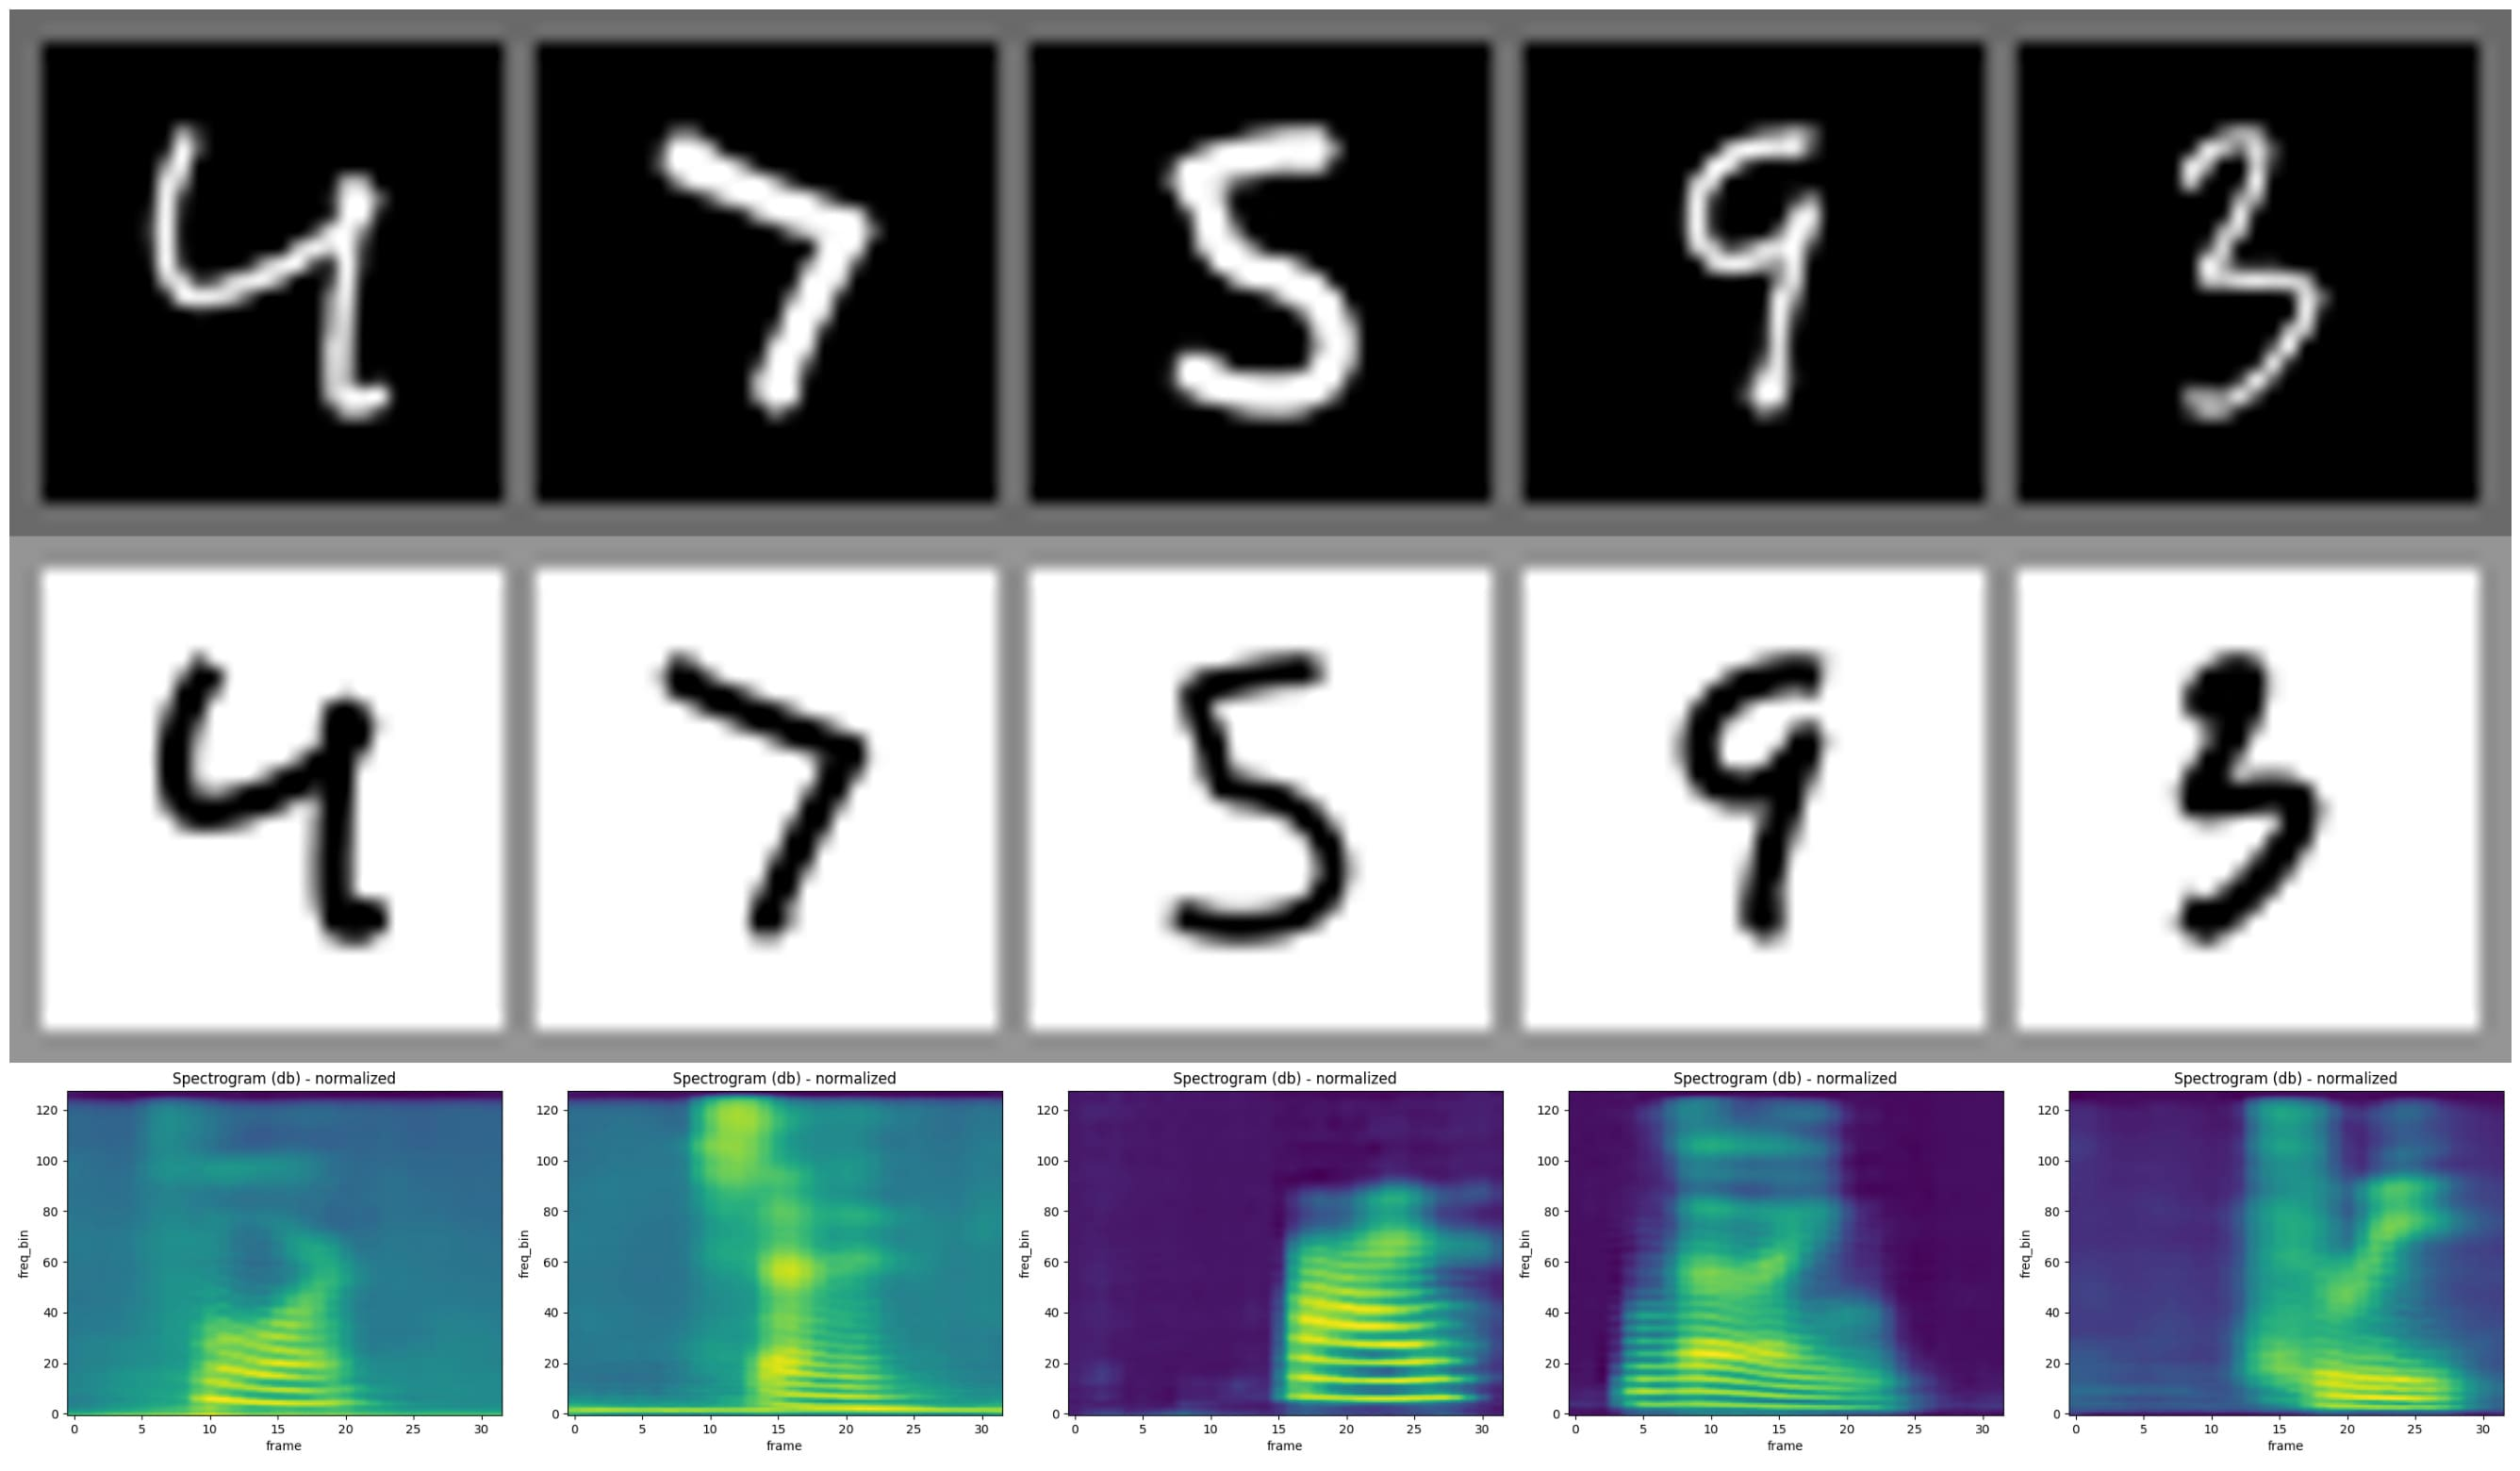
\includegraphics[page=1,width=\linewidth]{figures/datasets/mhd/MLD_sampling_mhd}
         \caption*{ \textbf{\gls{MLD} (ours)} }
     \end{subfigure}
     
        \caption{Joint generation qualitative results for \textbf{\mhd}. The three modalities are randomly generated simultaneously (\textbf{Top row}: image,\textbf{Middle row}: trajectory vector converted into image, \textbf{Bottom row}: sound Mel-Spectogram ).   }
        \label{fig:joint_mhd}
\end{figure}





\begin{figure}[H]
     \centering
       \centering
\begin{subfigure}{0.20\textwidth}
         \centering
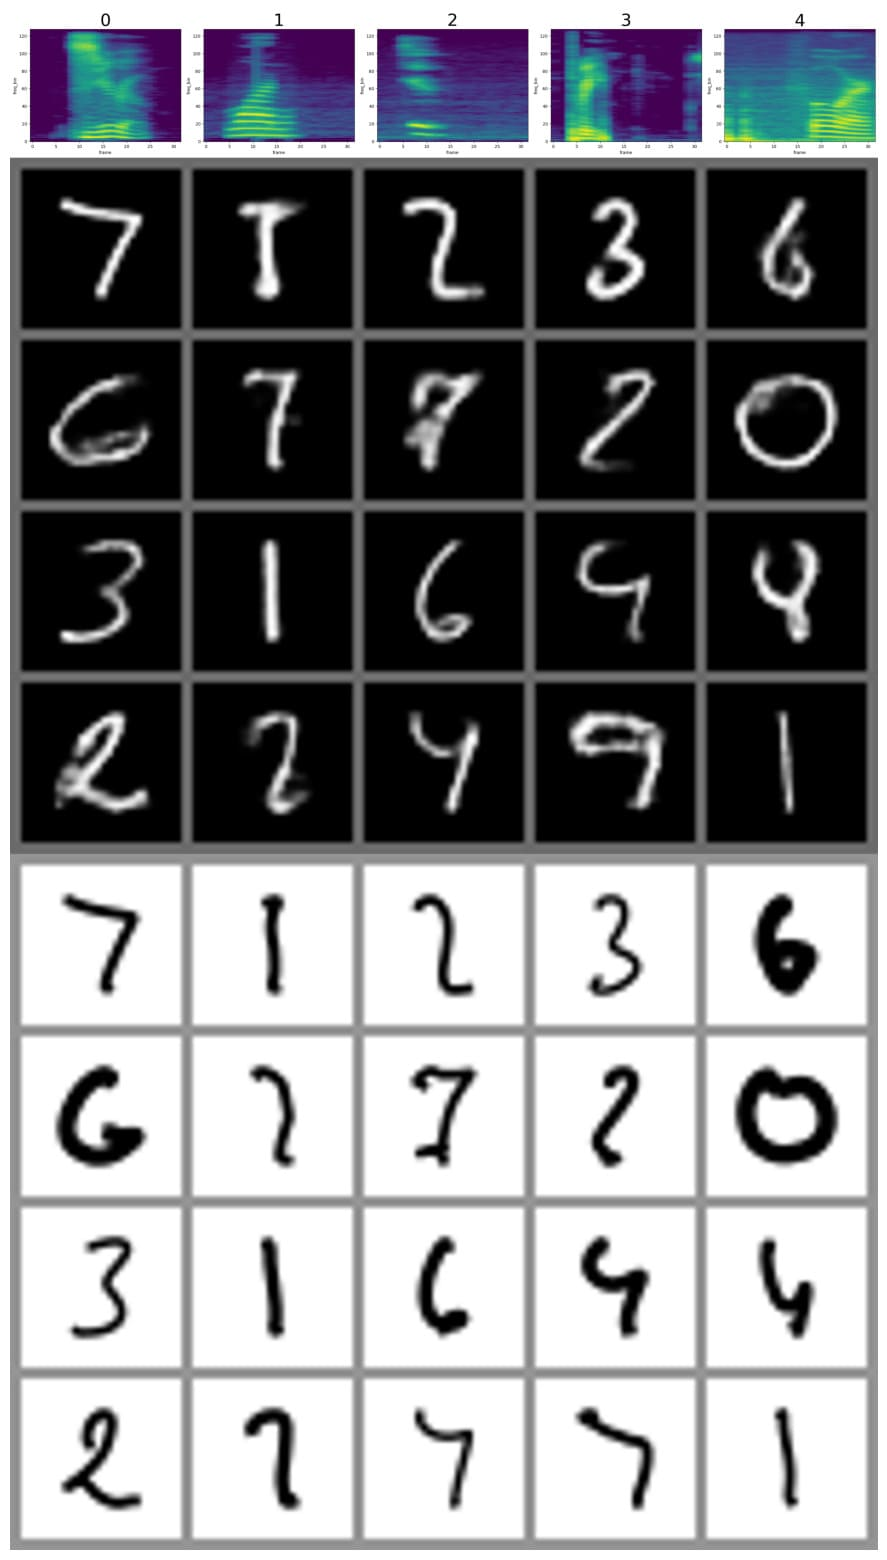
\includegraphics[width=\linewidth]{figures/datasets/mhd/mvae_cond_mhd}
  \caption*{\gls{MVAE}}
\end{subfigure}
\begin{subfigure}{0.20\textwidth}
         \centering
         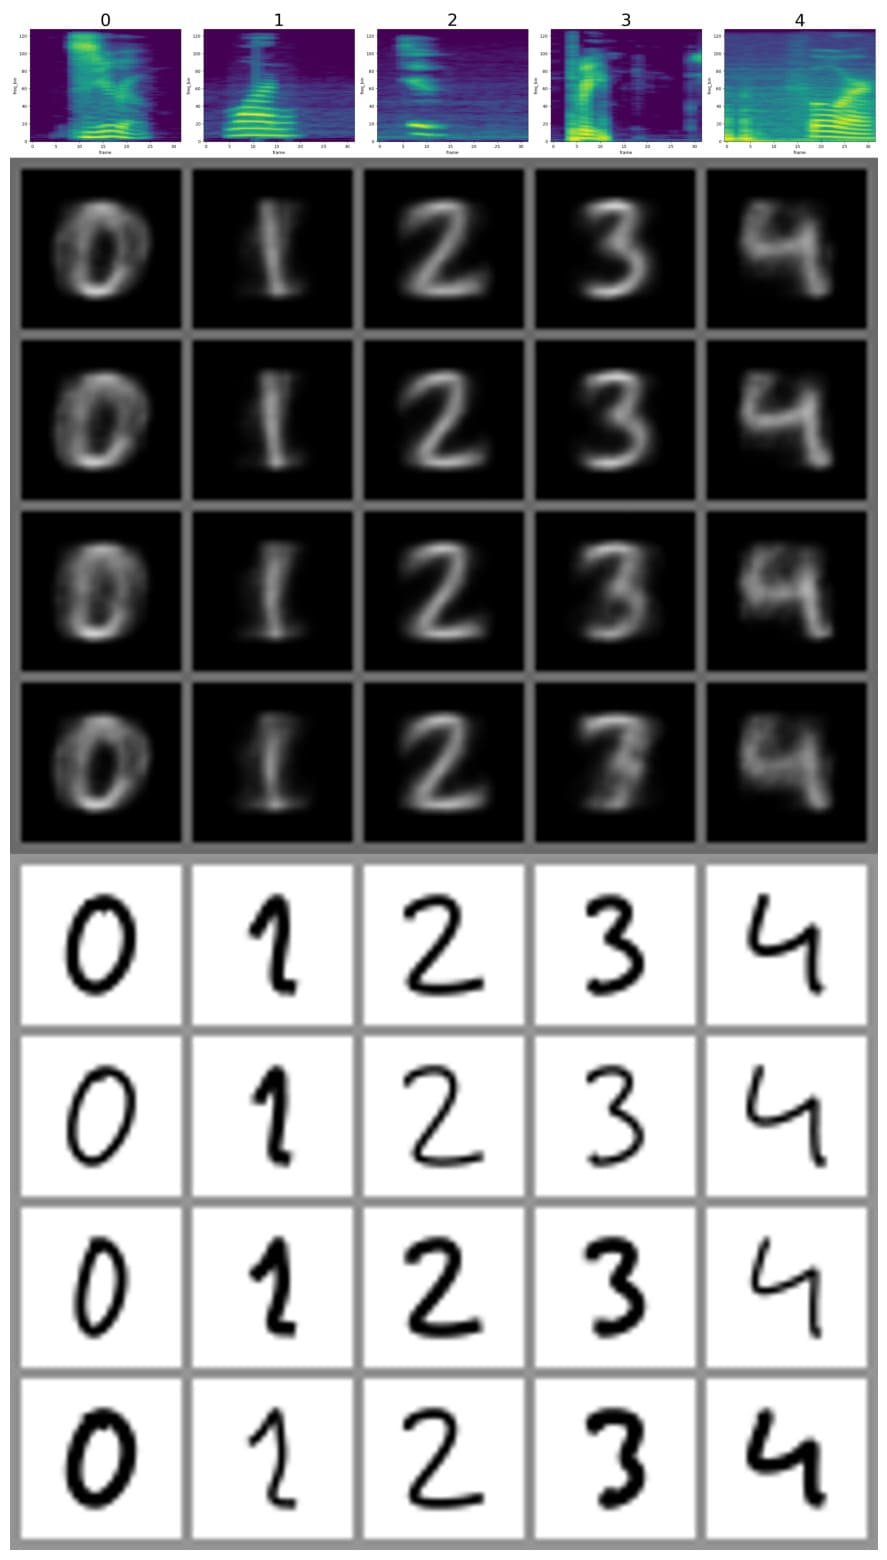
\includegraphics[width=\linewidth]{figures/datasets/mhd/mmvae_cond_mhd}
   \caption*{\gls{MMVAE}}
\end{subfigure}
\begin{subfigure}{0.20\textwidth}
         \centering
         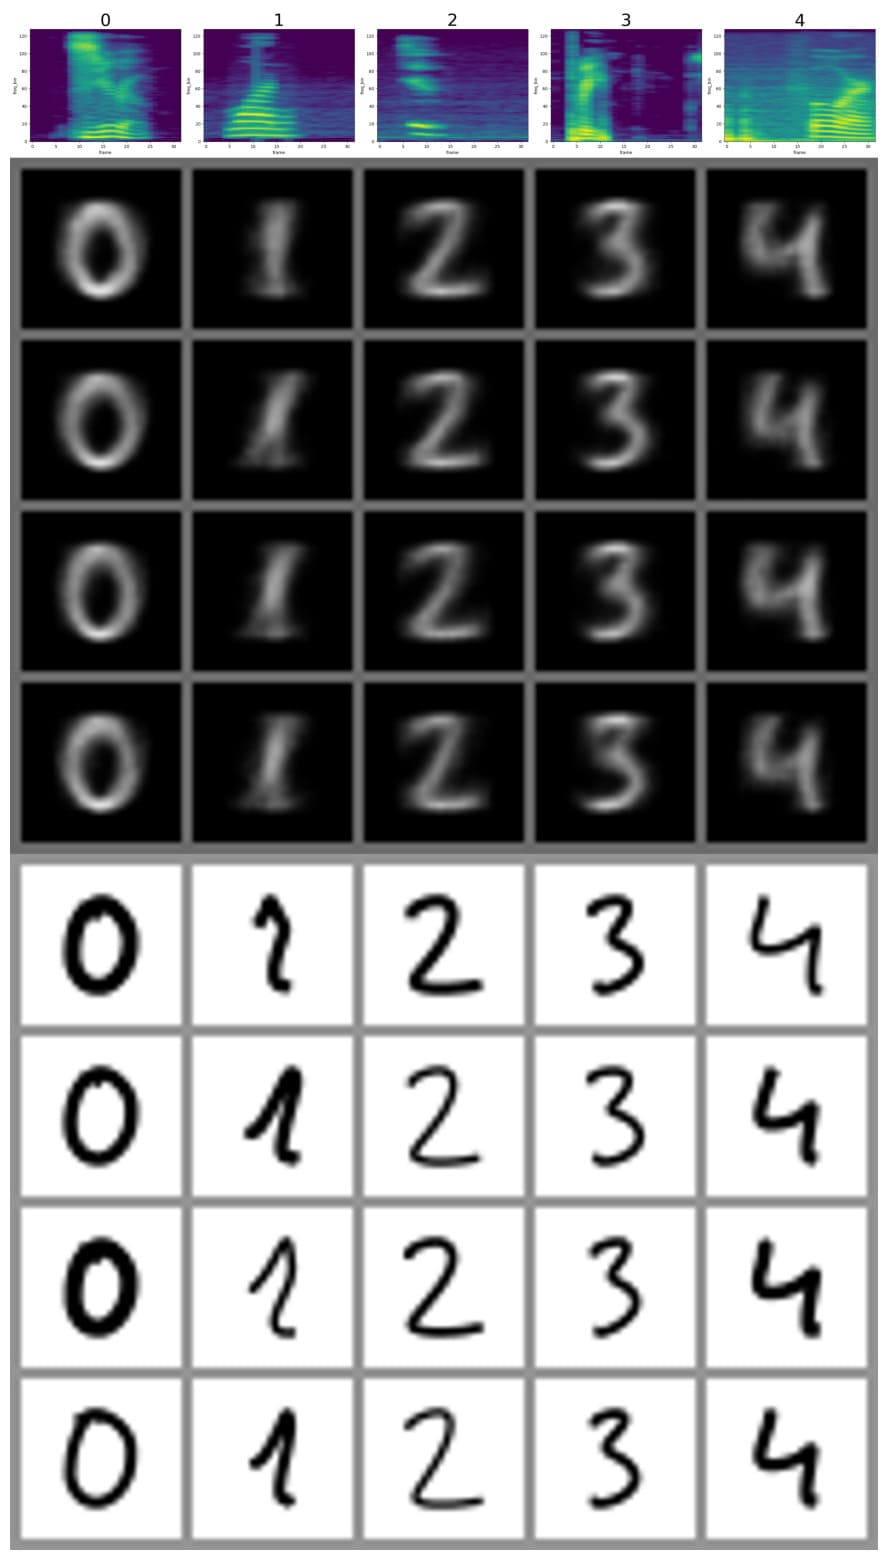
\includegraphics[width=\linewidth]{figures/datasets/mhd/mopoe_cond_mhd}
         \caption*{\gls{MOPOE}}
\end{subfigure}
\begin{subfigure}{0.20\textwidth}
         \centering
         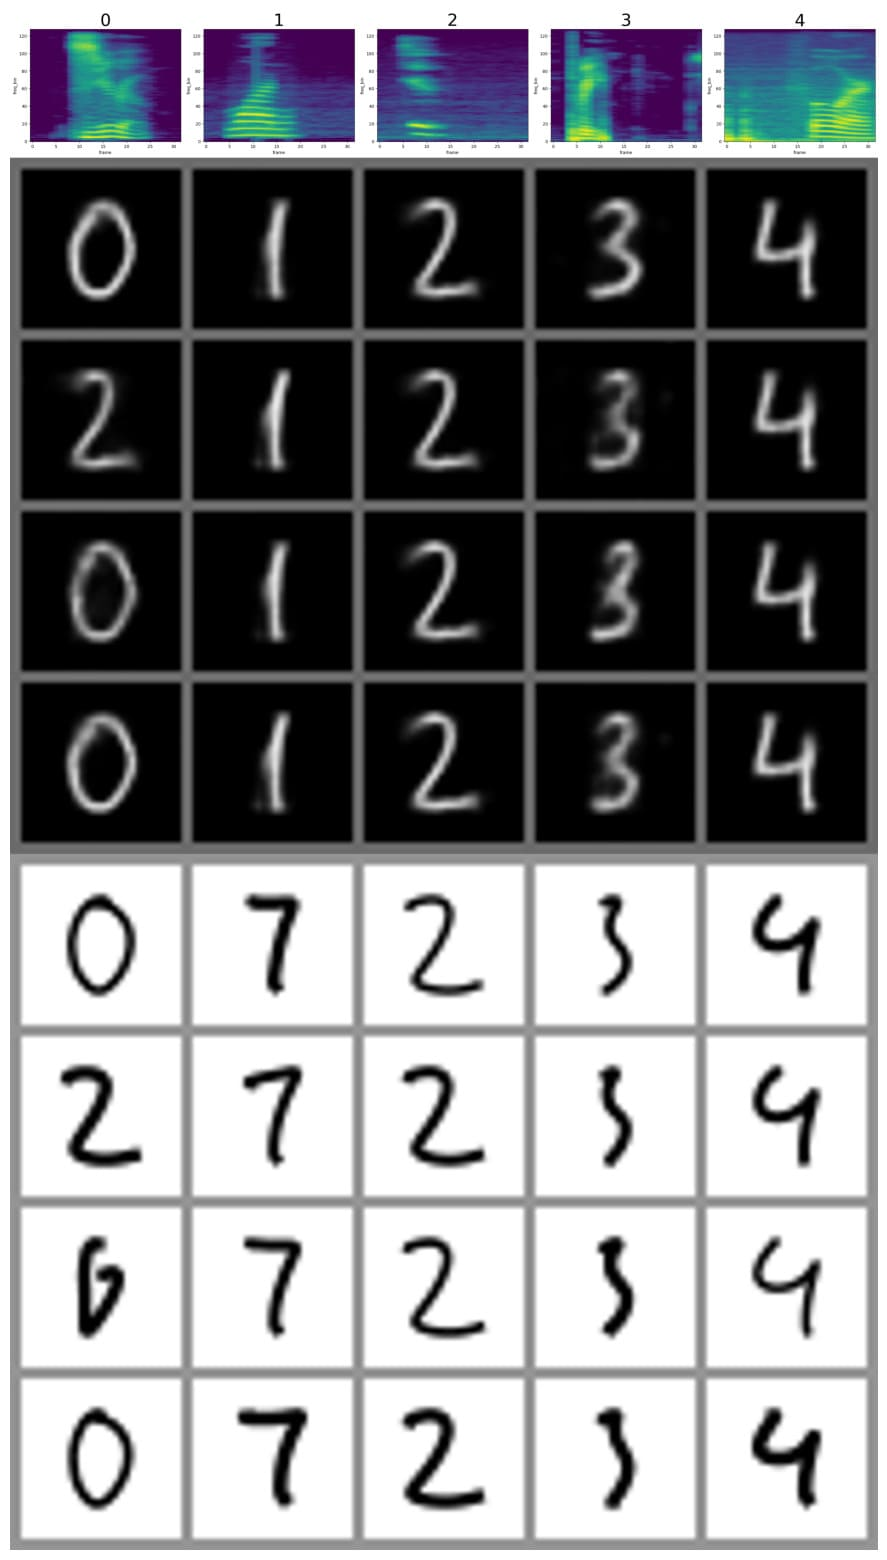
\includegraphics[width=\linewidth]{figures/datasets/mhd/nexus_cond_mhd}
         \caption*{\gls{NEXUS}}
     \end{subfigure}
     
\begin{subfigure}{0.20\textwidth}
         \centering
         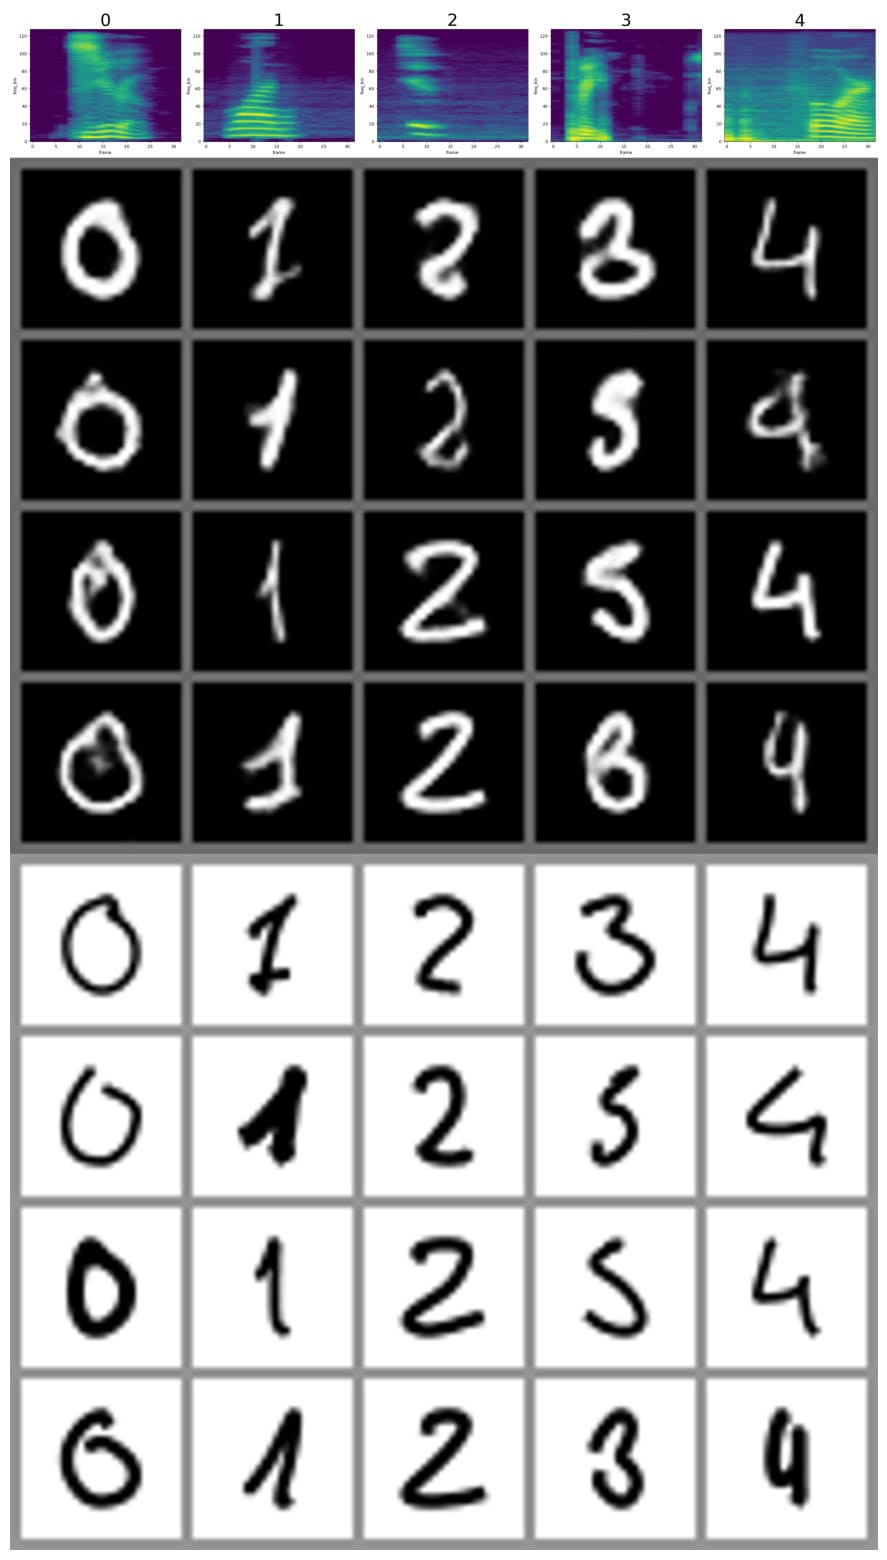
\includegraphics[width=\linewidth]{figures/datasets/mhd/tcmvae_cond_mhd}
         \caption*{\gls{MVTCAE}}
\end{subfigure}
% \begin{subfigure}{0.20\textwidth}
%          \centering
%          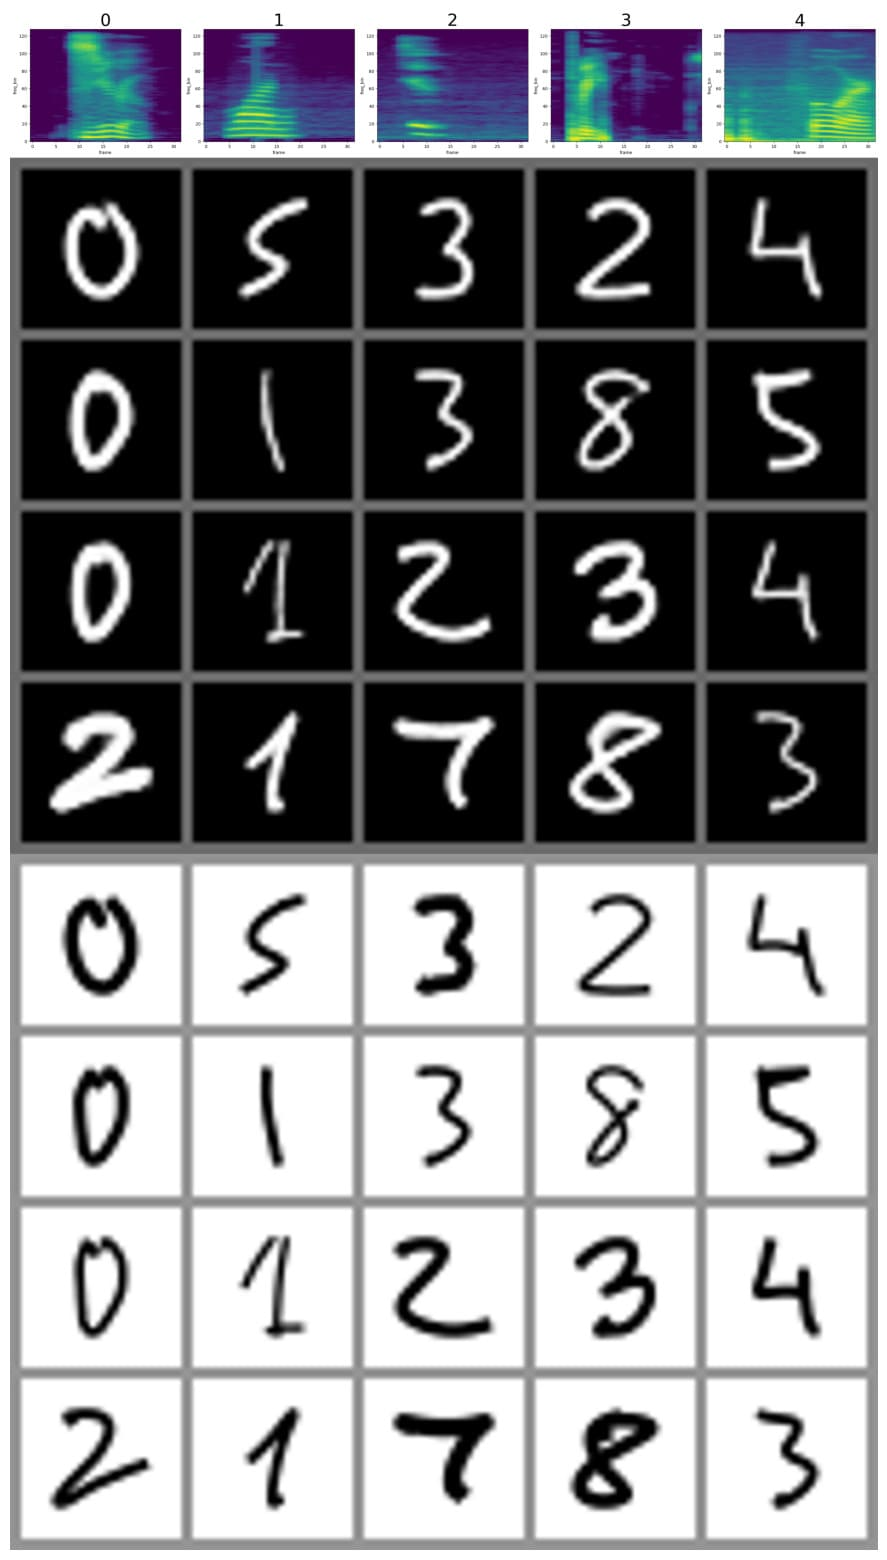
\includegraphics[page=1,width=\linewidth]{figures/datasets/mhd/MLD_inpaint_cond_mhd}
%          \caption*{\gls{MLD Inpaint} }
%      \end{subfigure}
%   \begin{subfigure}{0.20\textwidth}
%          \centering
%          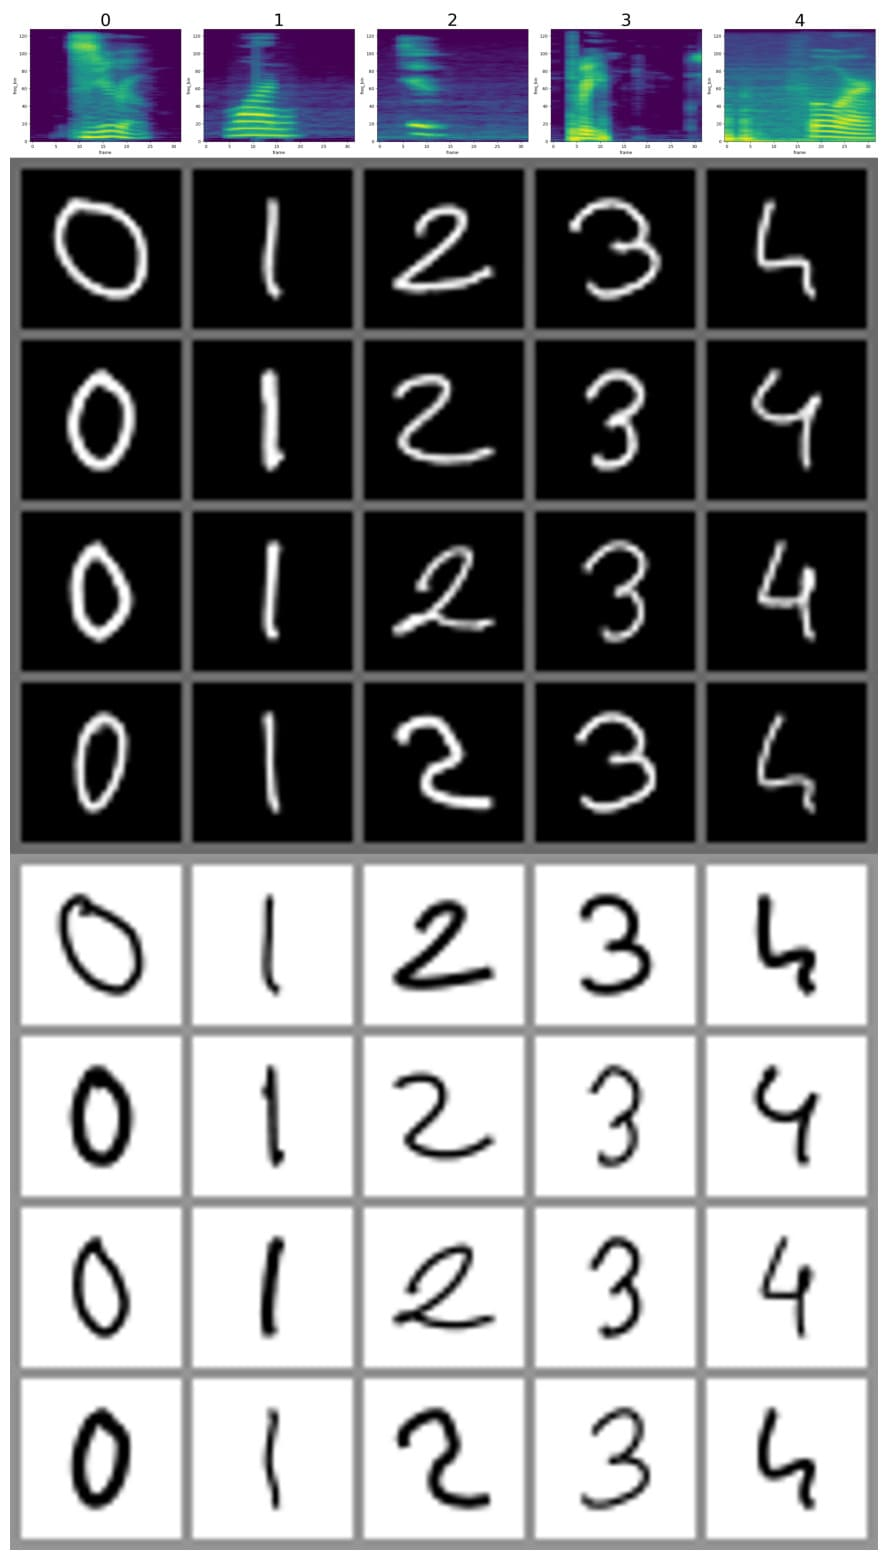
\includegraphics[page=1,width=\linewidth]{figures/datasets/mhd/MLD_uni_cond_mhd}
%          \caption*{\gls{MLD Uni} }
%      \end{subfigure}
  \begin{subfigure}{0.20\textwidth}
         \centering
         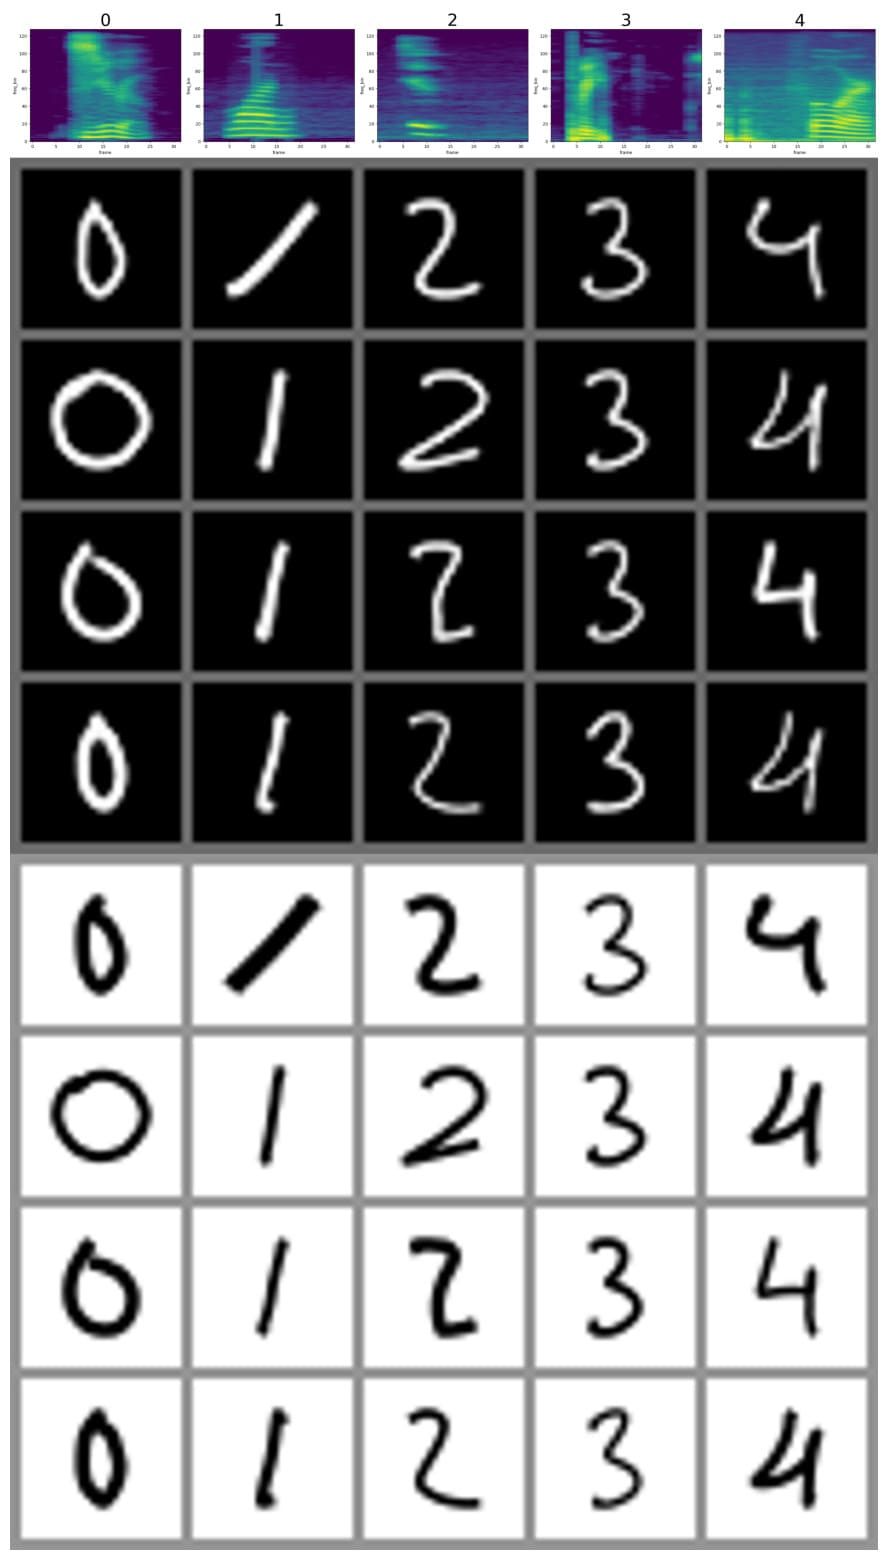
\includegraphics[page=1,width=\linewidth]{figures/datasets/mhd/MLD_cond_mhd}
         \caption*{ \textbf{\gls{MLD} (ours)} }
     \end{subfigure}
     
        \caption{ Sound to image and trajectory conditional generation qualitative results for \textbf{\mhd}. For each model we report: In the \textbf{Top row}, the sound mel-spectograms of the digits \{0,1,2,3,4\} from the left to the right, in \textbf{the rows below}, the generated images and trajectories samples.   }
        \label{fig:cond_mhd}
\end{figure}









\subsection{POLYMNIST}


\begin{table}[H]

\caption{Generation Coherence (\%) for \textbf{\polymnist} (Higher is better) used for the plots in \Cref{fig:res_mmnist} and \Cref{fig:res_mmnist_mld}. We report the average \textit{leave one out coherence} as a function of the number of observed modalities. \textit{Joint} refers to random generation of the 5 modalities simultaneously.
\newline
}  
\centering
\resizebox{0.8\textwidth}{!}{\begin{tabular}{c|c|cccc}
\toprule
\multirow{2}{*}{ Models }    &  \multicolumn{5}{c}{Coherence (\%$\uparrow$)}\\
    \cmidrule{2-6}
     &Joint  & 1 &  2 & 3 & 4   \\
    \midrule
    \gls{MVAE} &  $4.0_{ \pm 1.49 }$ & $37.51_{\pm 3.16 }$ & $ 48.06_{\pm 3.55}$ & $53.19_{ \pm3.37  }$  & $56.09 _{\pm  3.31 }$ \\
    \gls{MMVAE} &  $25.8_{ \pm 1.43 }$ & $\textbf{75.15}_{\pm 2.54}$ & $ 75.14_{\pm2.47}$ & $75.09_{ \pm2.6  }$  & $75.09 _{\pm  2.58 }$    \\

   \gls{MOPOE} & $ 17.32_{ \pm 2.47 }$ &
   $\underline{69.37}_{\pm 1.85}$ &
   $\underline{81.29}_{\pm 2.34}$ &
   $85.26_{ \pm 2.36  }$  & 
   $86.7 _{\pm 2.39 }$      \\
 
    \gls{NEXUS} &$ 18.24_{ \pm 0.89 }$ &
    $  60.61_{ \pm 2.51 }$ &
    $ 72.14_{ \pm 2.79 }$ & 
    $ 76.81_{ \pm 2.75 }$ &
    $ 78.92_{ \pm 2.64}$ \\
    

    \gls{MVTCAE} & $0.21_{\pm 0.05 }$ & 
    $57.66_{\pm 1.06 }$ &
    $78.44_{\pm1.31} $&
    $\underline{85.97}_{\pm 1.43} $&
    $\underline{88.81}_{ \pm 1.49  }$ \\

    \gls{MMVAEplus} &  $26.28_{\pm 2.19 }$ & 
    $54.74_{\pm 0.5 }$ &
    $54.06_{\pm0.33} $&
    $55.2_{\pm 1.32} $&
    $53.17_{ \pm0.75 }$ \\

    \gls{MMVAEplus} (K=10)&  $14.53_{\pm 4.94 }$ & 
    $58.93_{\pm 6.3 }$ &
    $59.42_{\pm8.8} $&
    $60.77_{\pm 8.03} $&
    $58.24_{ \pm 7.42  }$ \\
    

    \midrule
    \gls{MLD Inpaint} & $\underline{51.65}_{\pm 1.16 }$ &  $52.85_{\pm 0.23 }$ &
    $77.65_{\pm0.24} $& 
    $85.66_{\pm 0.43} $&
    $87.29_{ \pm 0.29  }$ \\
    

    \gls{MLD Uni} & 
    $48.79_{\pm 0.43 }$ &  
    $65.12_{\pm 0.7 }$ &
    $79.52_{\pm0.8} $&
    $82.03_{\pm 1.19} $&
    $81.86_{ \pm 2.09  }$ 
    \\

    \gls{MLD} & $\textbf{56.23}_{ \pm 0.52}$ & $68.58_{\pm 0.72} $&$ \textbf{84.87}_{\pm 0.19}$ & $\textbf{88.56}_{ \pm 0.12} $ &$ \textbf{89.43}_{\pm 0.27}  $ \\
    
    \bottomrule
\end{tabular}}
\label{tab:mmnist_detail}
\end{table}





\begin{table}[H]
\caption{Generation quality (\gls{FID} $\downarrow$) for \textbf{\polymnist} (lower is better) used for the plots in \Cref{fig:res_mmnist} and \Cref{fig:res_mmnist_mld}. Similar to \Cref{tab:mmnist_detail}, we report the average \textit{leave one out} \gls{FID} as a function of the number of observed modalities. \textit{Joint} refers to random generation quality of the 5 modalities simultaneously.
\newline
}  
\centering
\resizebox{0.8\textwidth}{!}{\begin{tabular}{c|c|cccc}
\toprule
\multirow{1}{*}{ Models }    &  \multicolumn{5}{c}{Quality ($\downarrow$)}\\
    \cmidrule{2-6}
     &Joint  & 1 &  2 & 3 & 4   \\
    \midrule
    \gls{MVAE} &  $108.74_{ \pm 2.73 }$ & $108.06_{\pm 2.79 }$ & $ 108.05_{\pm 2.73}$ & $108.14_{ \pm2.71  }$  & $108.18_{\pm  2.85 }$ \\

   \gls{MMVAE} &  $165.74_{ \pm 5.4}$ & $208.16_{\pm 10.41 }$ & $ 207.5_{\pm10.57}$ & $207.35_{ \pm10.59 }$  & $207.38_{\pm10.58 }$    \\
   \gls{MOPOE} & $ 113.77_{ \pm 1.62 }$ & $173.87_{\pm 7.34 }$ & $185.06_{\pm 10.21}$ & $191.72_{ \pm 11.26  }$  & $196.17
 _{\pm 11.66}$      \\
    \gls{NEXUS} & $ 91.66_{ \pm 2.93 }$ & $207.14_{\pm 7.71 }$ & $205.54_{\pm 8.6}$ & $204.46_{ \pm 9.08  }$  & $202.43
 _{\pm 9.49}$     \\
    \gls{MVTCAE} &
    $106.55_{\pm 3.83  } $ & $78.3_{\pm2.35} $  &   $85.55_{\pm2.51 }$&   $92.73_{\pm2.65 }$&   $99.13_{\pm2.72 }$\\

     \gls{MMVAEplus} &  $168.88_{\pm 0.12 }$ & 
    $165.67_{\pm 0.14 }$ &
    $166.5_{\pm0.18} $&
    $165.53_{\pm 0.55} $&
    $165.3_{ \pm0.33 }$ \\

    \gls{MMVAEplus} (K=10)&  $156.55_{\pm 3.58 }$ & 
    $154.42_{\pm 2.73 }$ &
    $153.1_{\pm3.01} $&
    $153.06_{\pm 2.88} $&
    $154.9_{ \pm 2.9  }$ \\
    
    \midrule
    \gls{MLD Inpaint} &   $64.78_{\pm0.33 }$&
    $65.41_{\pm 0.43  } $ & $65.42_{\pm0.41} $  &   $65.52_{\pm0.46 }$&   $\underline{65.55}_{\pm0.46 }$\\
    
    \gls{MLD Uni} &   $\textbf{62.42}_{\pm0.62 }$&
    $\underline{63.16}_{\pm 0.81  } $ & $\underline{64.09}_{\pm1.15} $  &   $\underline{65.17}_{\pm1.46 }$&   $66.46_{\pm2.18 }$\\
     
    \gls{MLD} & 
    $\underline{63.05}_{\pm0.26}$   &   $ \textbf{62.89}_{\pm 0.2}$ &
     $\textbf{62.53}_{\pm0.21}$   &   $\textbf{62.22}_{\pm 0.39}$ &   $\textbf{61.94}_{\pm0.65}$ \\
    \bottomrule
\end{tabular}}

\end{table}





\begin{figure} [H]
     \centering
     \begin{subfigure}{0.19\textwidth}
        \begin{subfigure}{1\textwidth}
         \centering
         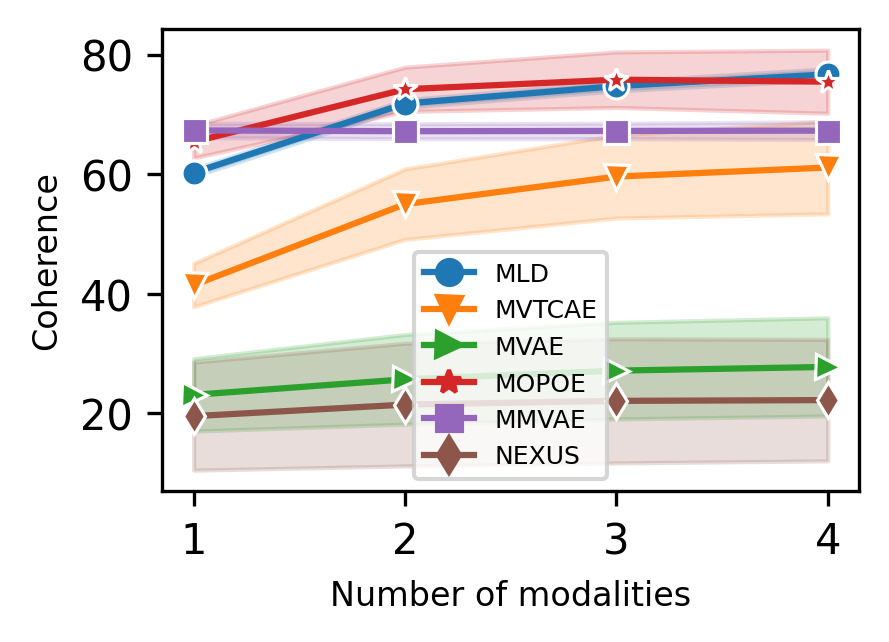
\includegraphics[page=1,width=\linewidth]{figures/datasets/mmnist/quant/mld_baseline_mmnist_coh_m0}

        \end{subfigure} 
          \begin{subfigure}{1\textwidth}
         \centering
         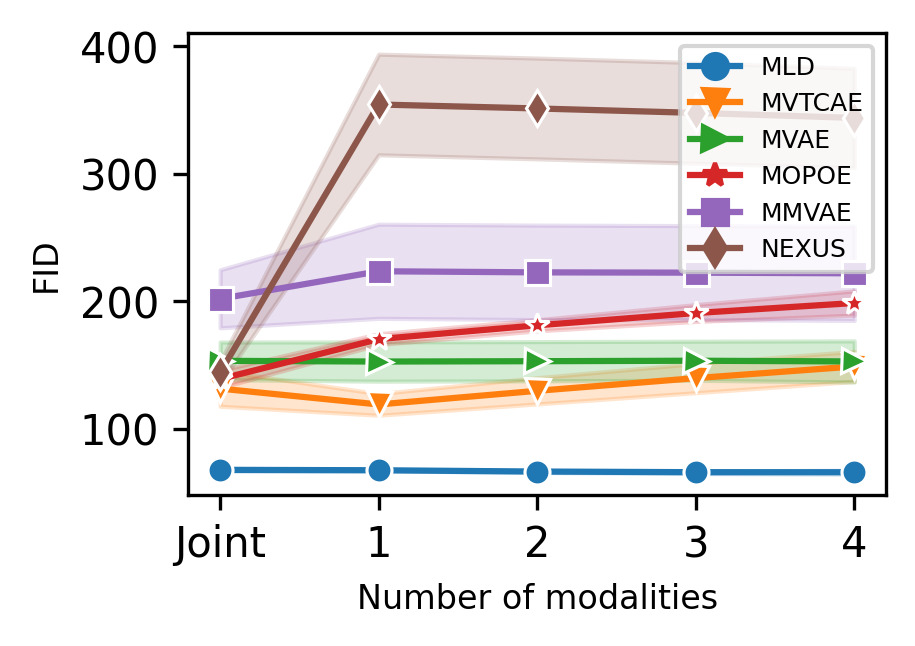
\includegraphics[page=1,width=\linewidth]{figures/datasets/mmnist/quant/mld_baseline_mmnist_plot_fid_m0}

        \end{subfigure} 
        \caption{$X^0$}
     \end{subfigure} 
   \begin{subfigure}{0.19\textwidth}
        \begin{subfigure}{1\textwidth}
         \centering
         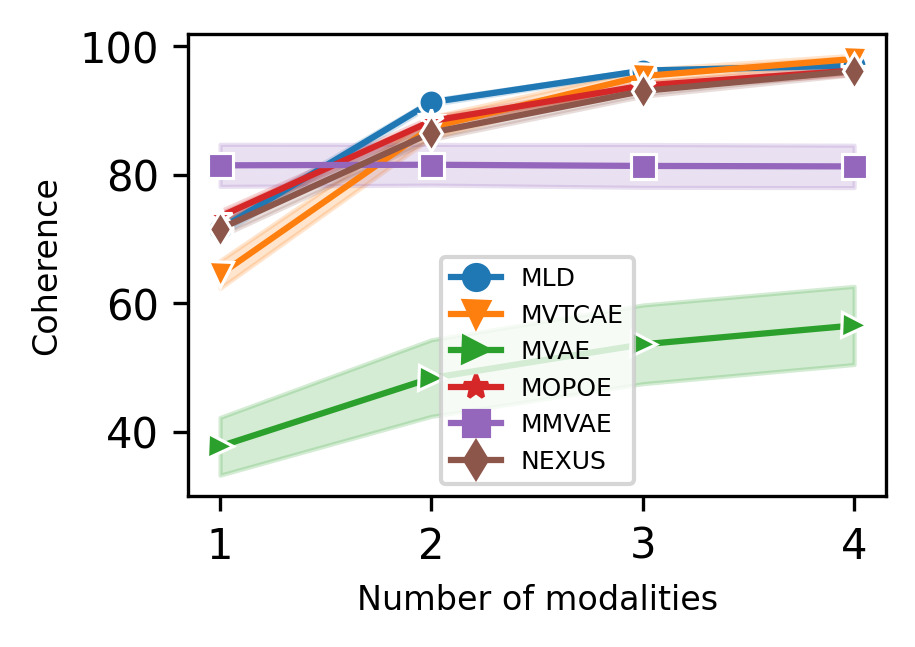
\includegraphics[page=1,width=\linewidth]{figures/datasets/mmnist/quant/mld_baseline_mmnist_coh_m1}

        \end{subfigure} 
          \begin{subfigure}{1\textwidth}
         \centering
         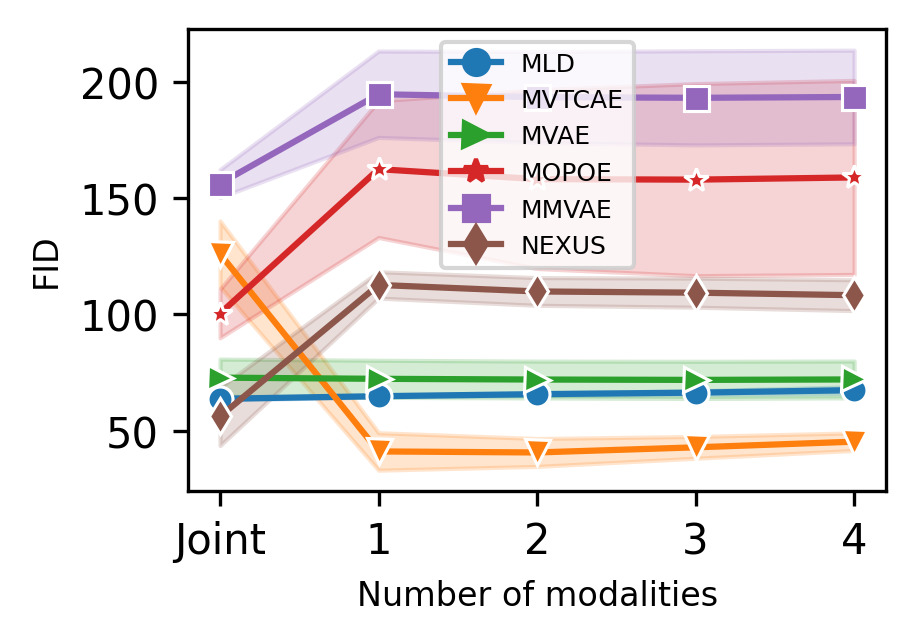
\includegraphics[page=1,width=\linewidth]{figures/datasets/mmnist/quant/mld_baseline_mmnist_plot_fid_m1}
   
        \end{subfigure} 

        \caption{$X^1$}
     \end{subfigure}
     \begin{subfigure}{0.19\textwidth}
        \begin{subfigure}{1\textwidth}
         \centering
         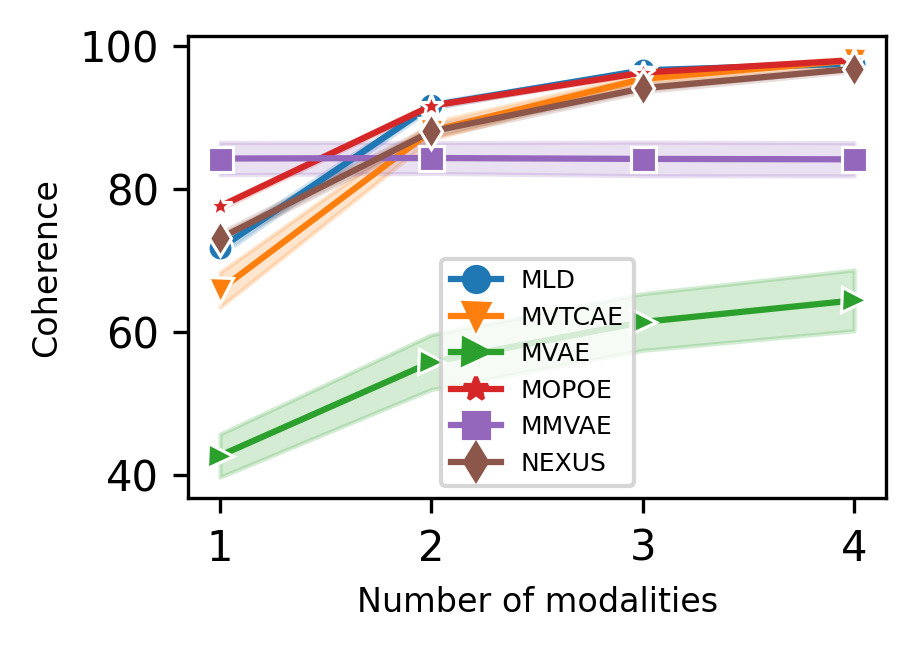
\includegraphics[page=1,width=\linewidth]{figures/datasets/mmnist/quant/mld_baseline_mmnist_coh_m2}

        \end{subfigure} 
          \begin{subfigure}{1\textwidth}
         \centering
         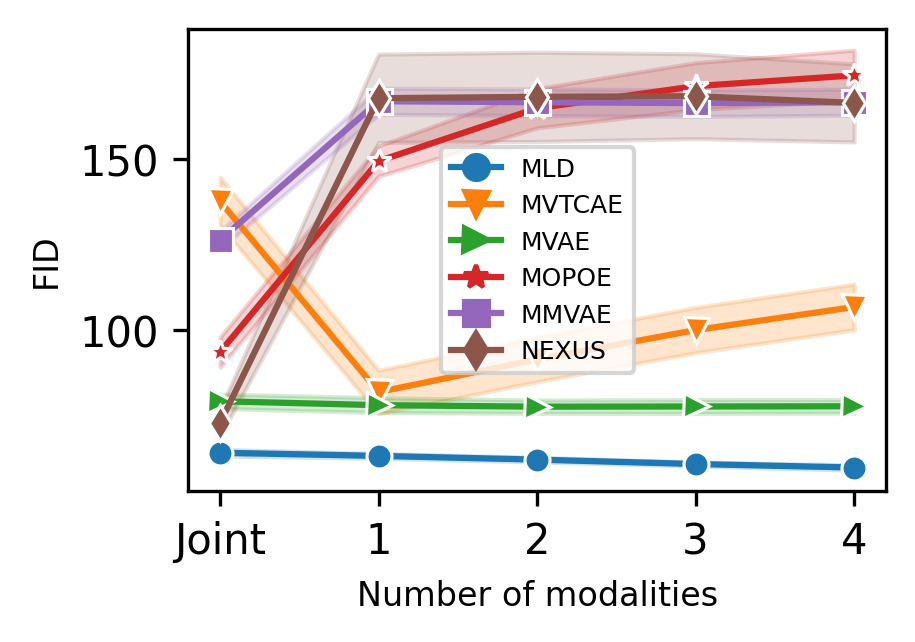
\includegraphics[page=1,width=\linewidth]{figures/datasets/mmnist/quant/mld_baseline_mmnist_plot_fid_m2}

        \end{subfigure} 
        \caption{$X^2$}
     \end{subfigure}
      \begin{subfigure}{0.19\textwidth}
        \begin{subfigure}{1\textwidth}
         \centering
         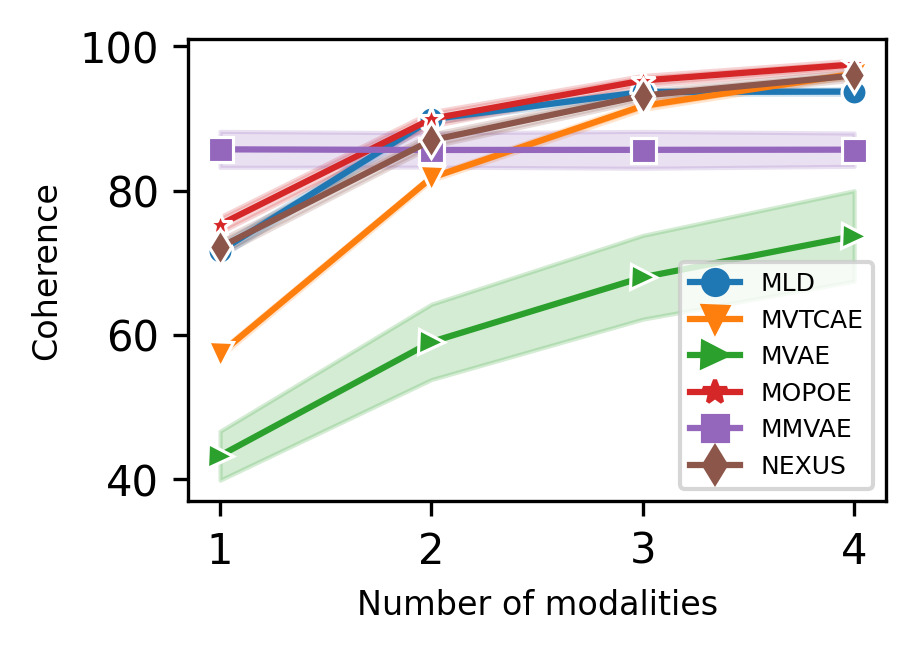
\includegraphics[page=1,width=\linewidth]{figures/datasets/mmnist/quant/mld_baseline_mmnist_coh_m3}
    
        \end{subfigure} 
          \begin{subfigure}{1\textwidth}
         \centering
         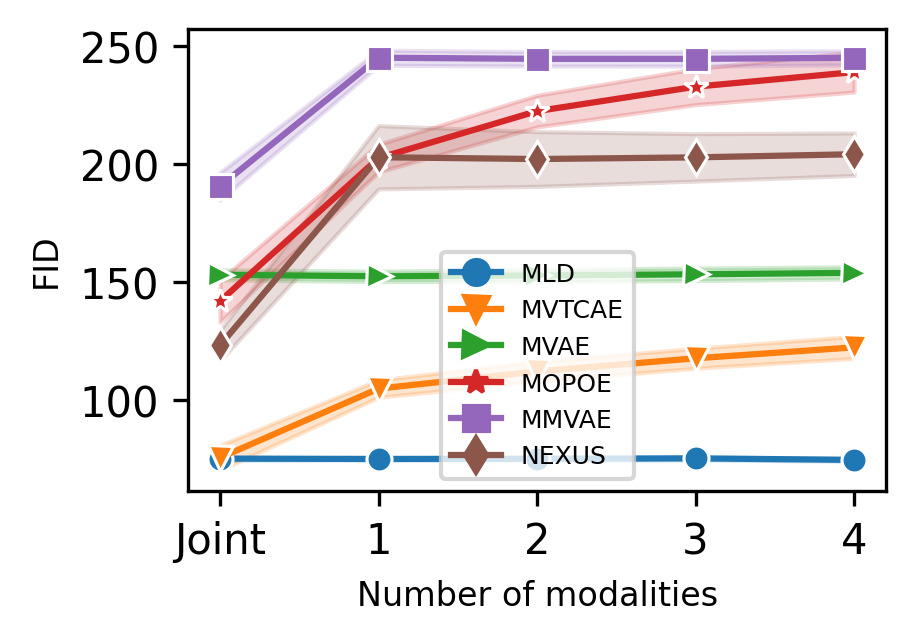
\includegraphics[page=1,width=\linewidth]{figures/datasets/mmnist/quant/mld_baseline_mmnist_plot_fid_m3}
    
        \end{subfigure} 
        \caption{$X^3$}
     \end{subfigure}
     \begin{subfigure}{0.19\textwidth}
        \begin{subfigure}{1\textwidth}
         \centering
         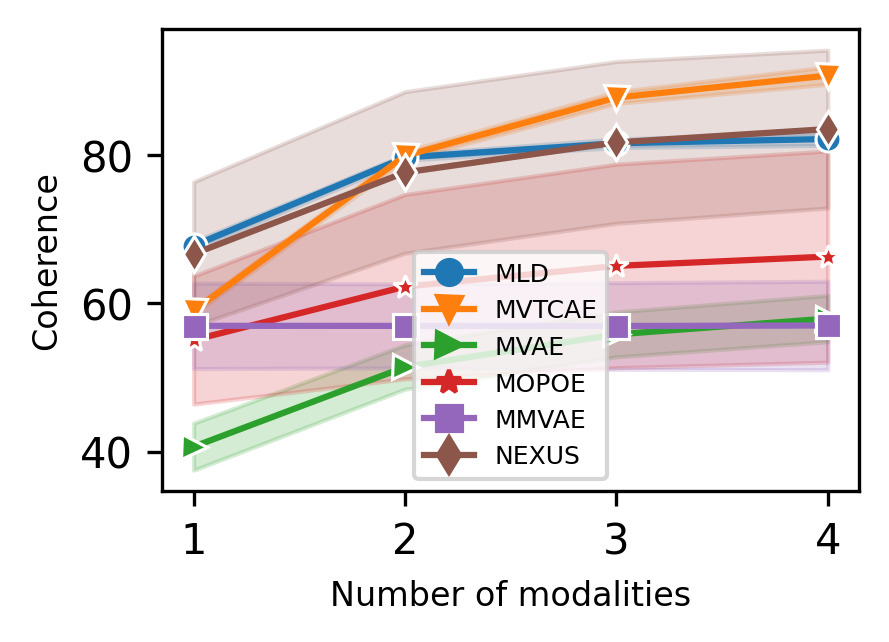
\includegraphics[page=1,width=\linewidth]{figures/datasets/mmnist/quant/mld_baseline_mmnist_coh_m4}
         
        \end{subfigure} 
          \begin{subfigure}{1\textwidth}
         \centering
         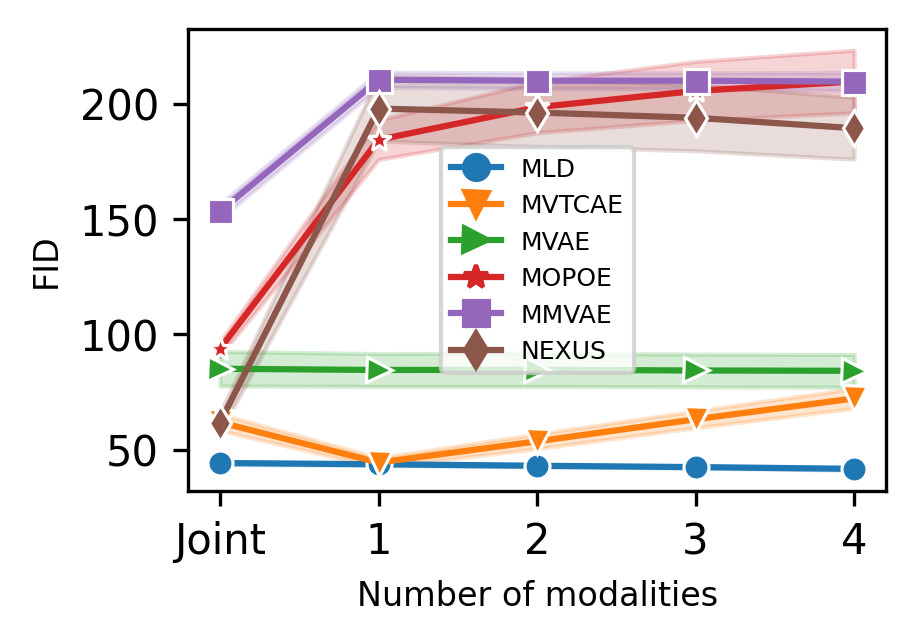
\includegraphics[page=1,width=\linewidth]{figures/datasets/mmnist/quant/mld_baseline_mmnist_plot_fid_m4}
        
        \end{subfigure} 
        \caption{$X^4$}
     \end{subfigure}
\caption{ \textbf{Top:} Generation Coherence (\%) for \textbf{\polymnist} (Higher is better). \textbf{Bottom:} Generation quality (\gls{FID}) (Lower is better). We report the average \textit{leave one out} performance as a function of the number of observed modalities for each modality $X^i$. \textit{Joint} refers to random generation of the 5 modalities simultaneously.}
        \label{res:mmnist_mld_var_mod}
\end{figure}





\begin{figure} [H]
     \centering
     \begin{subfigure}{0.19\textwidth}
        \begin{subfigure}{1\textwidth}
         \centering
         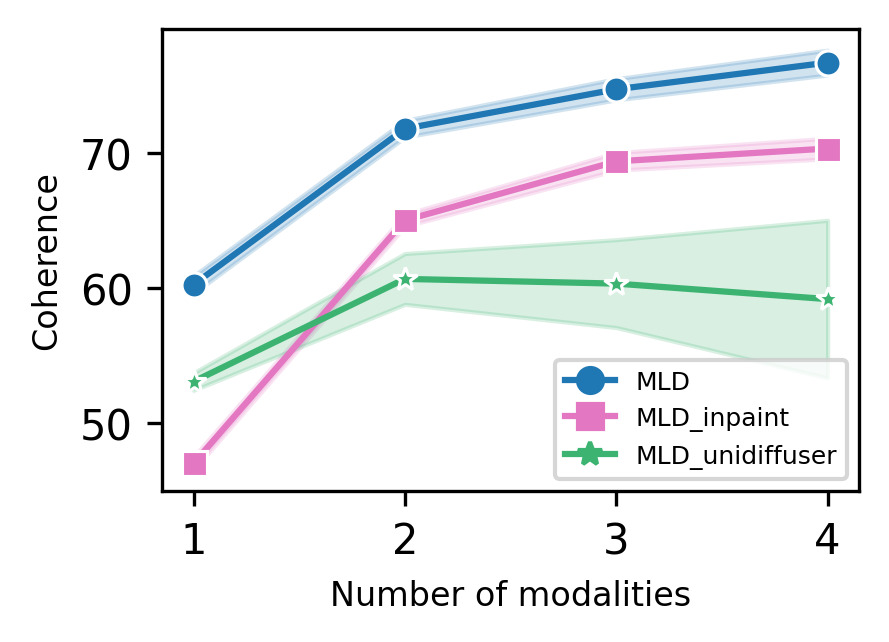
\includegraphics[page=1,width=\linewidth]{figures/datasets/mmnist/quant/mld_variants_mmnist_plot_coh_m0}
     
        \end{subfigure} 
          \begin{subfigure}{1\textwidth}
         \centering
         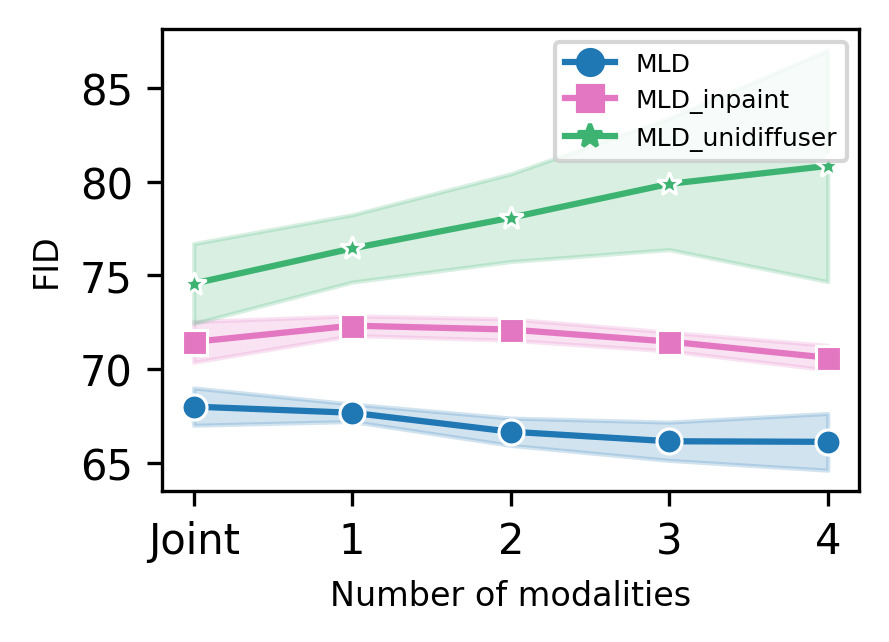
\includegraphics[page=1,width=\linewidth]{figures/datasets/mmnist/quant/mld_variants_mmnist_plot_fid_m0}

        \end{subfigure} 
        \caption{$X^0$}
     \end{subfigure} 
   \begin{subfigure}{0.19\textwidth}
        \begin{subfigure}{1\textwidth}
         \centering
         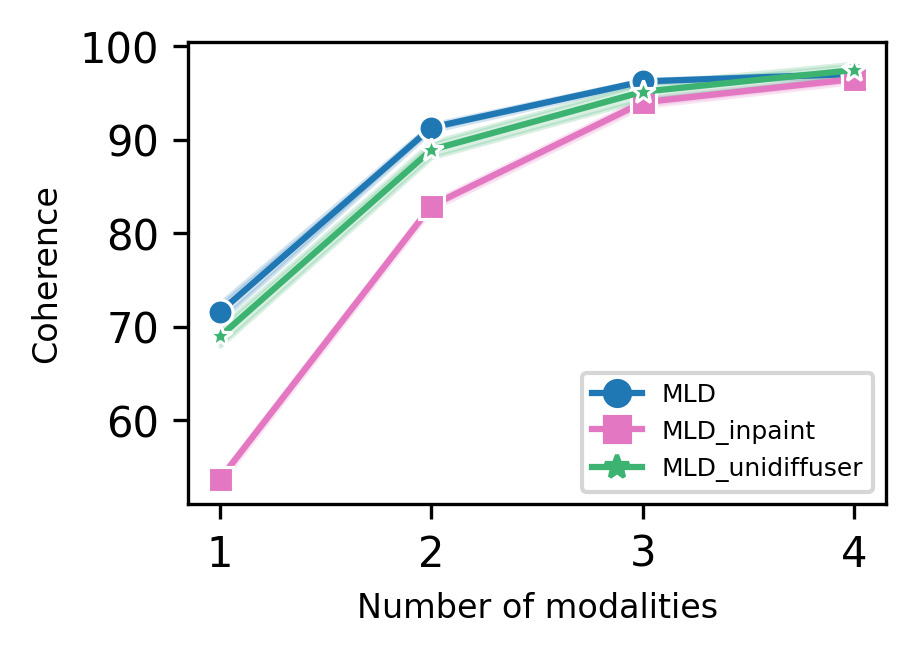
\includegraphics[page=1,width=\linewidth]{figures/datasets/mmnist/quant/mld_variants_mmnist_plot_coh_m1}
   
        \end{subfigure} 
          \begin{subfigure}{1\textwidth}
         \centering
         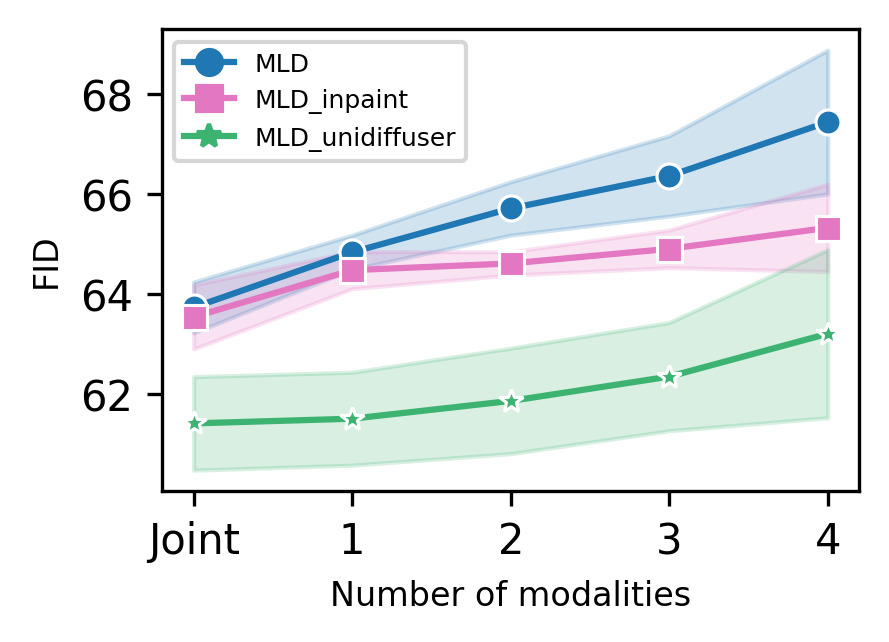
\includegraphics[page=1,width=\linewidth]{figures/datasets/mmnist/quant/mld_variants_mmnist_plot_fid_m1}
   
        \end{subfigure} 

        \caption{$X^1$}
     \end{subfigure}
     \begin{subfigure}{0.19\textwidth}
        \begin{subfigure}{1\textwidth}
         \centering
         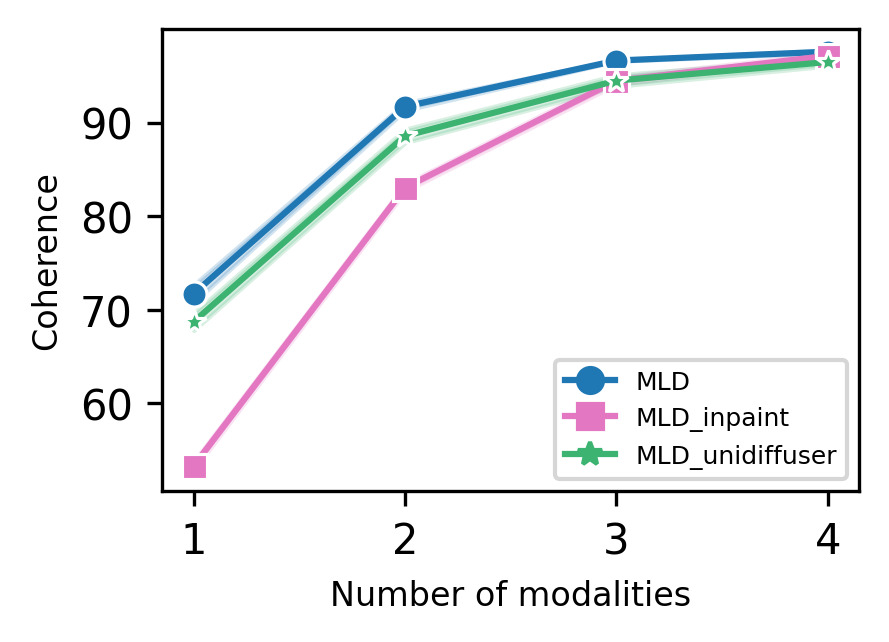
\includegraphics[page=1,width=\linewidth]{figures/datasets/mmnist/quant/mld_variants_mmnist_plot_coh_m2}

        \end{subfigure} 
          \begin{subfigure}{1\textwidth}
         \centering
         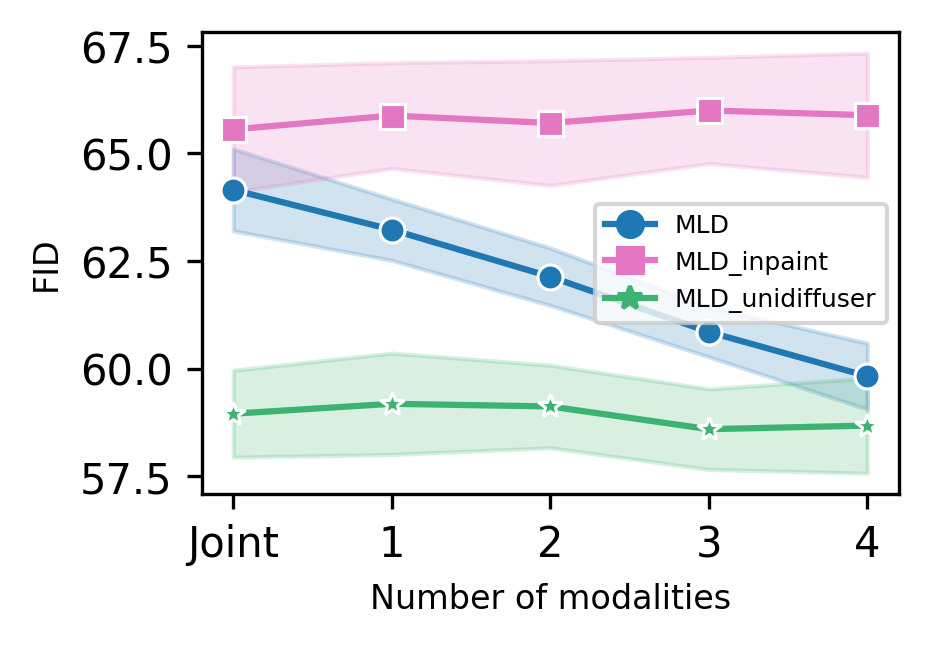
\includegraphics[page=1,width=\linewidth]{figures/datasets/mmnist/quant/mld_variants_mmnist_plot_fid_m2}

        \end{subfigure} 
        \caption{$X^2$}
     \end{subfigure}
      \begin{subfigure}{0.19\textwidth}
        \begin{subfigure}{1\textwidth}
         \centering
         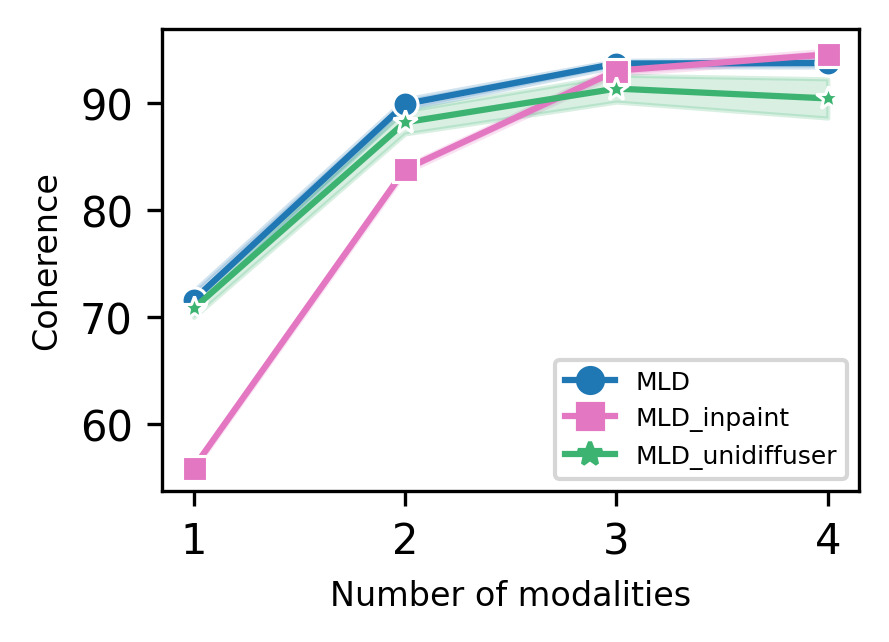
\includegraphics[page=1,width=\linewidth]{figures/datasets/mmnist/quant/mld_variants_mmnist_plot_coh_m3}
 
        \end{subfigure} 
          \begin{subfigure}{1\textwidth}
         \centering
         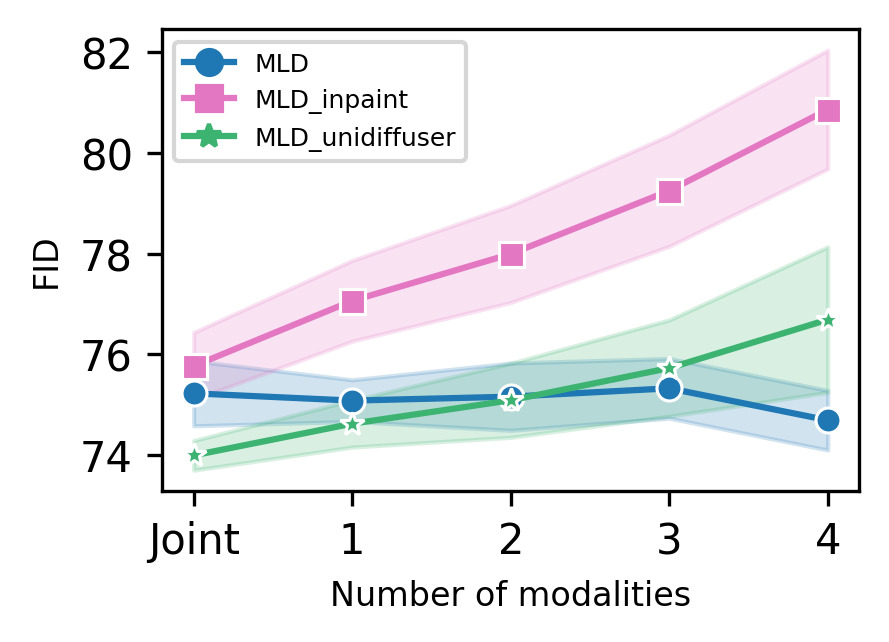
\includegraphics[page=1,width=\linewidth]{figures/datasets/mmnist/quant/mld_variants_mmnist_plot_fid_m3}

        \end{subfigure} 
        \caption{$X^3$}
     \end{subfigure}
     \begin{subfigure}{0.19\textwidth}
        \begin{subfigure}{1\textwidth}
         \centering
         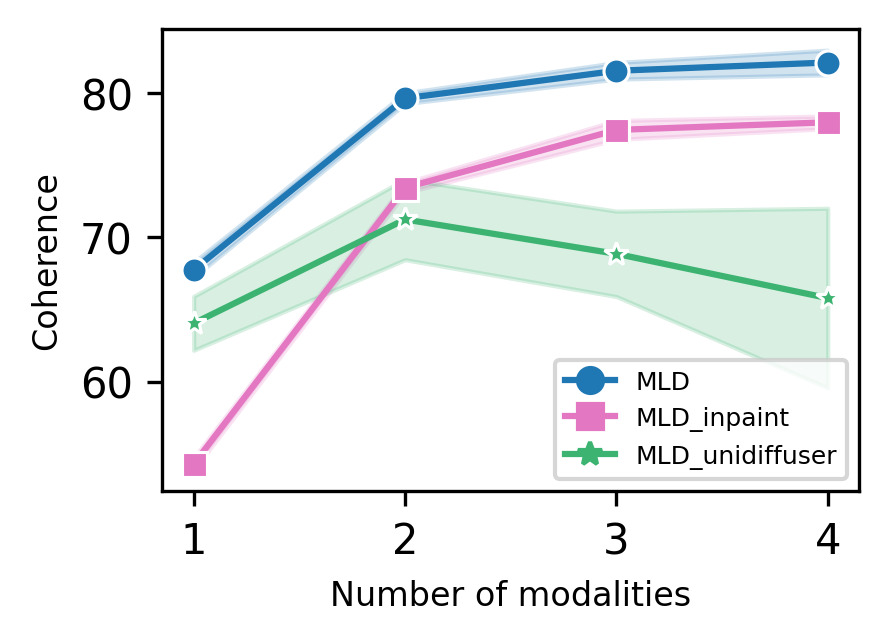
\includegraphics[page=1,width=\linewidth]{figures/datasets/mmnist/quant/mld_variants_mmnist_plot_coh_m4}
 
        \end{subfigure} 
          \begin{subfigure}{1\textwidth}
         \centering
         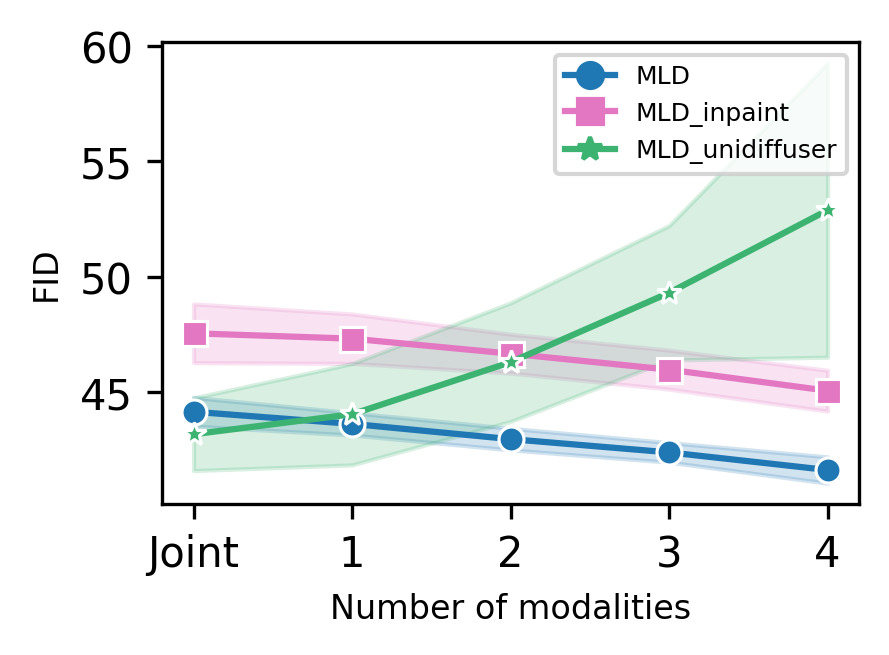
\includegraphics[page=1,width=\linewidth]{figures/datasets/mmnist/quant/mld_variants_mmnist_plot_fid_m4}
   
        \end{subfigure} 
        \caption{$X^4$}
     \end{subfigure}
        \caption{\textbf{Top:} Generation Coherence (\%) for \textbf{\polymnist} (Higher is better).\textbf{Bottom:} Generation quality (\gls{FID}) (Lower is better).
        We report the average \textit{leave one out} performance as a function of the number of observed modalities for each modality $X^i$. \textit{Joint} refers to random generation of the 5 modalities simultaneously.}
        \label{res:mmnist_mod}
\end{figure}








\begin{figure}[H]
     \centering
       \centering
     \begin{subfigure}{0.2\textwidth}
         \centering
         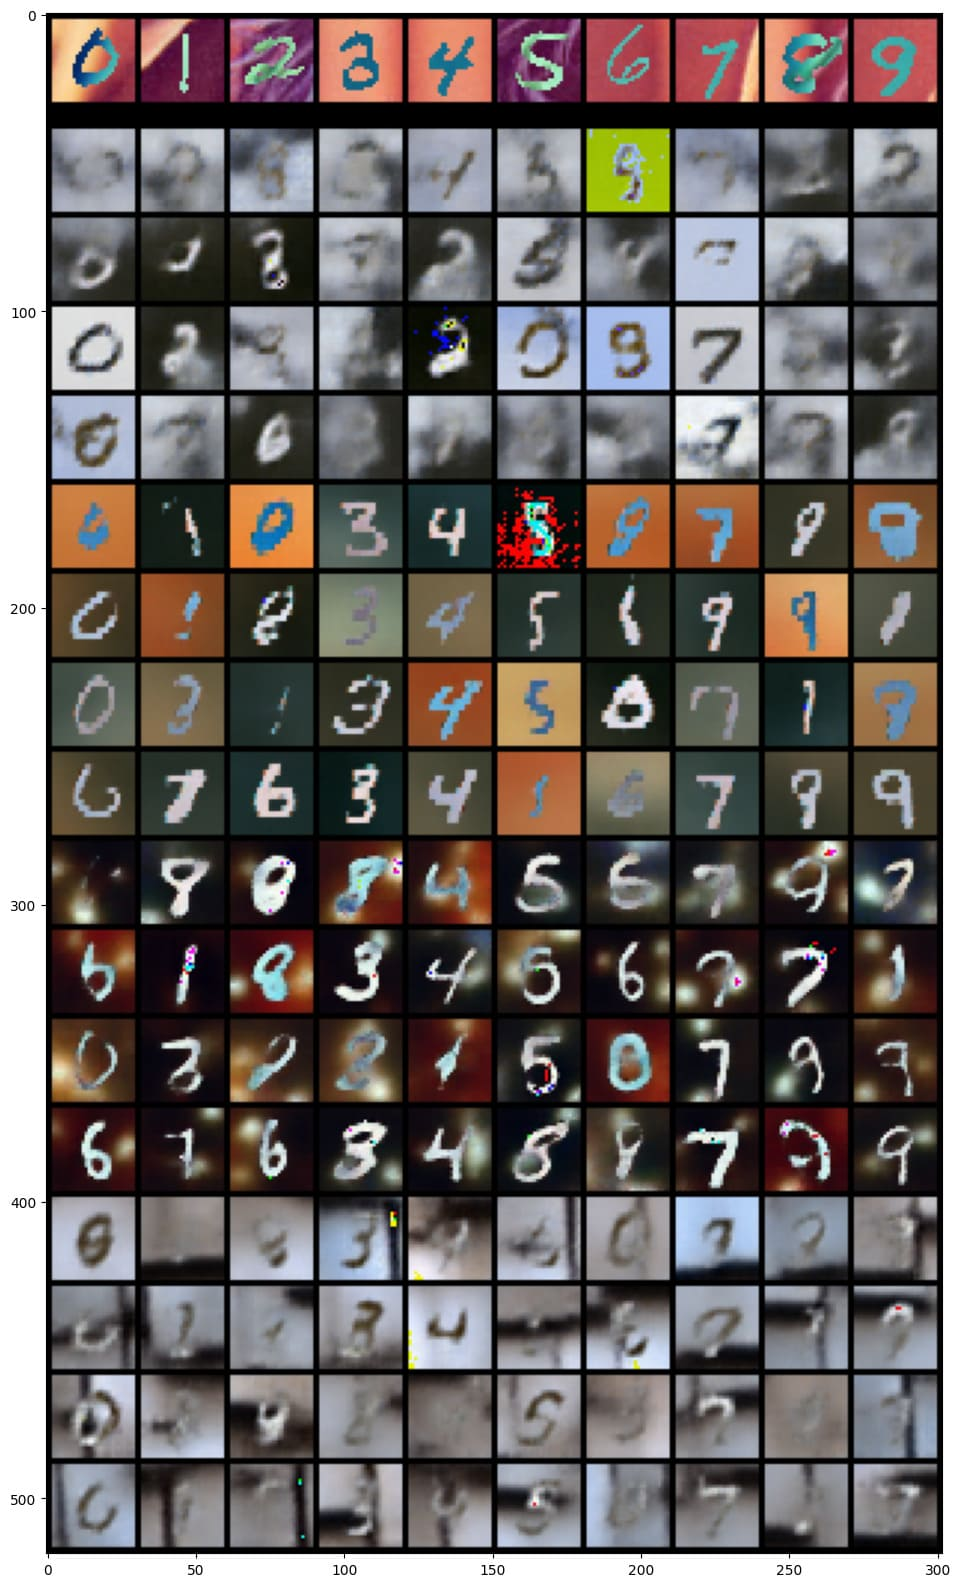
\includegraphics[width=\linewidth]{figures/datasets/mmnist/quali/mvae_cond_m2_out_remaining_mmnist}
  \caption*{\gls{MVAE}}
     \end{subfigure}
     \begin{subfigure}{0.2\textwidth}
         \centering
         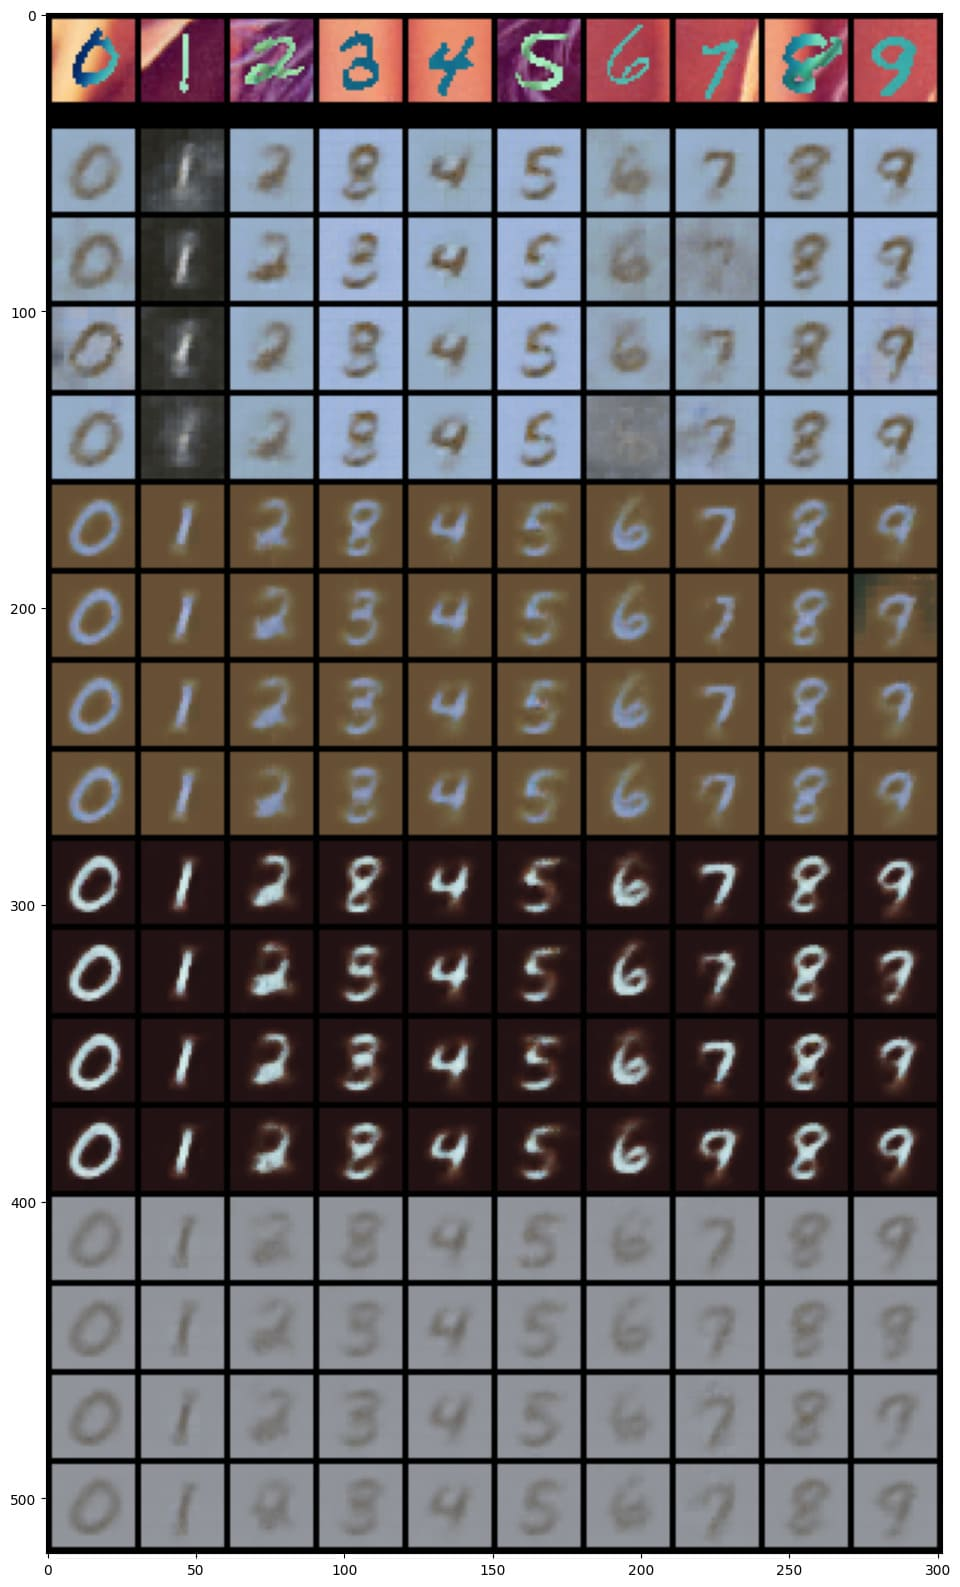
\includegraphics[width=\linewidth]{figures/datasets/mmnist/quali/mmvae_cond_m2_out_remaining_mmnist}
   \caption*{\gls{MMVAE}}
     \end{subfigure}
       \begin{subfigure}{0.2\textwidth}
         \centering
         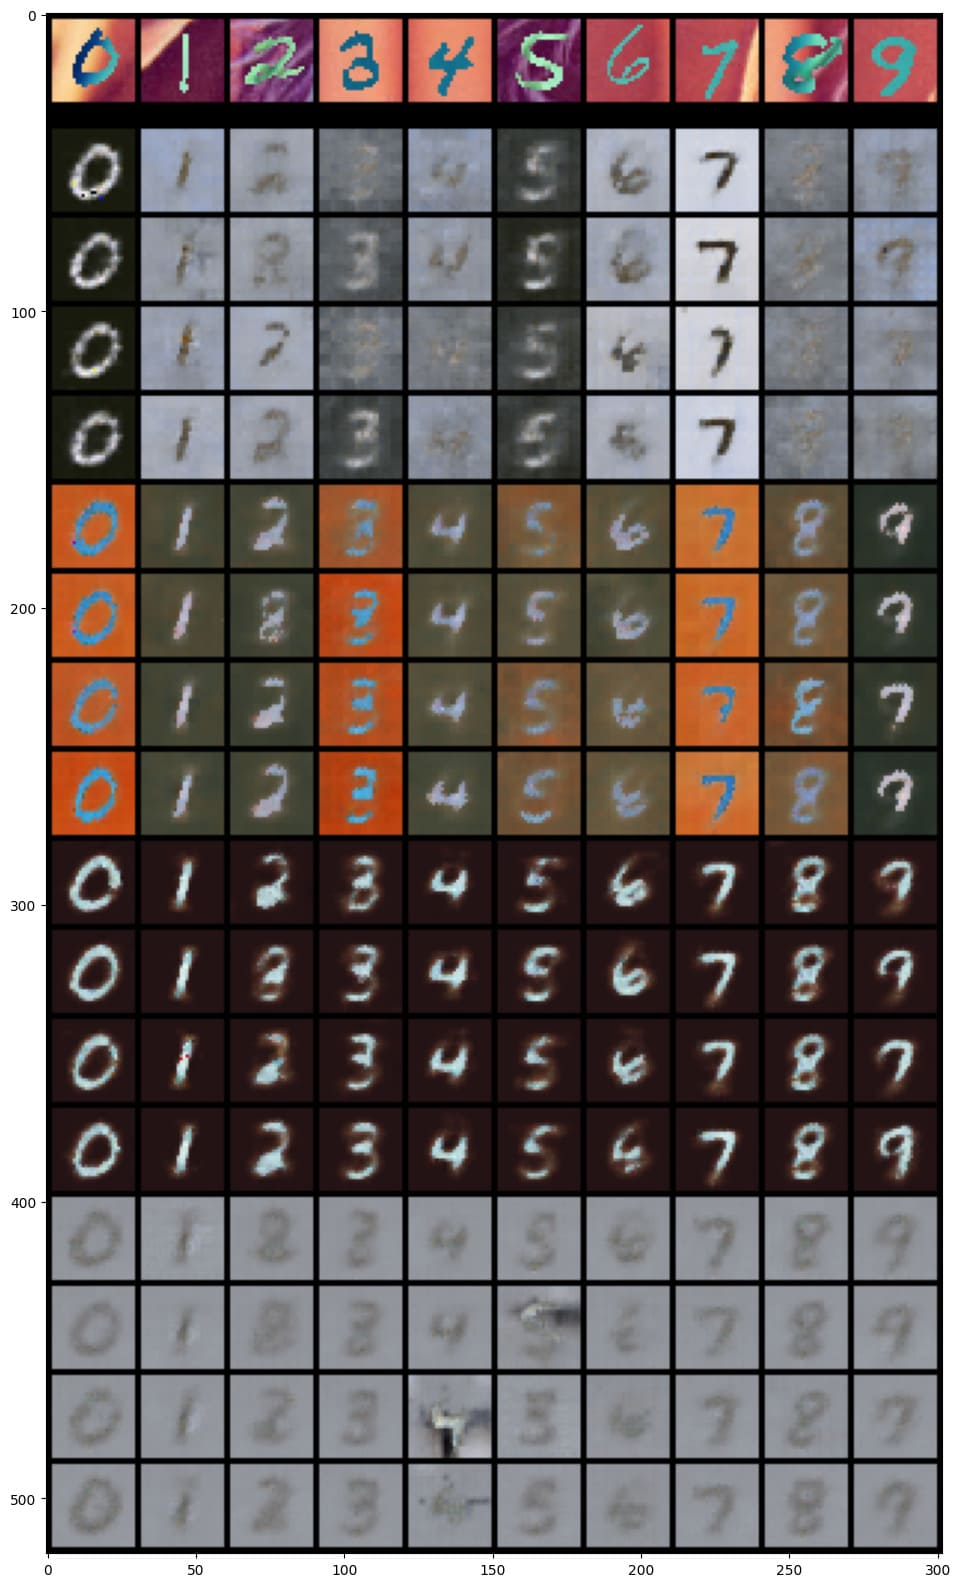
\includegraphics[width=\linewidth]{figures/datasets/mmnist/quali/mopoe_cond_m2_out_remaining_mmnist}
         \caption*{\gls{MOPOE}}

     \end{subfigure}
      \begin{subfigure}{0.2\textwidth}
         \centering
         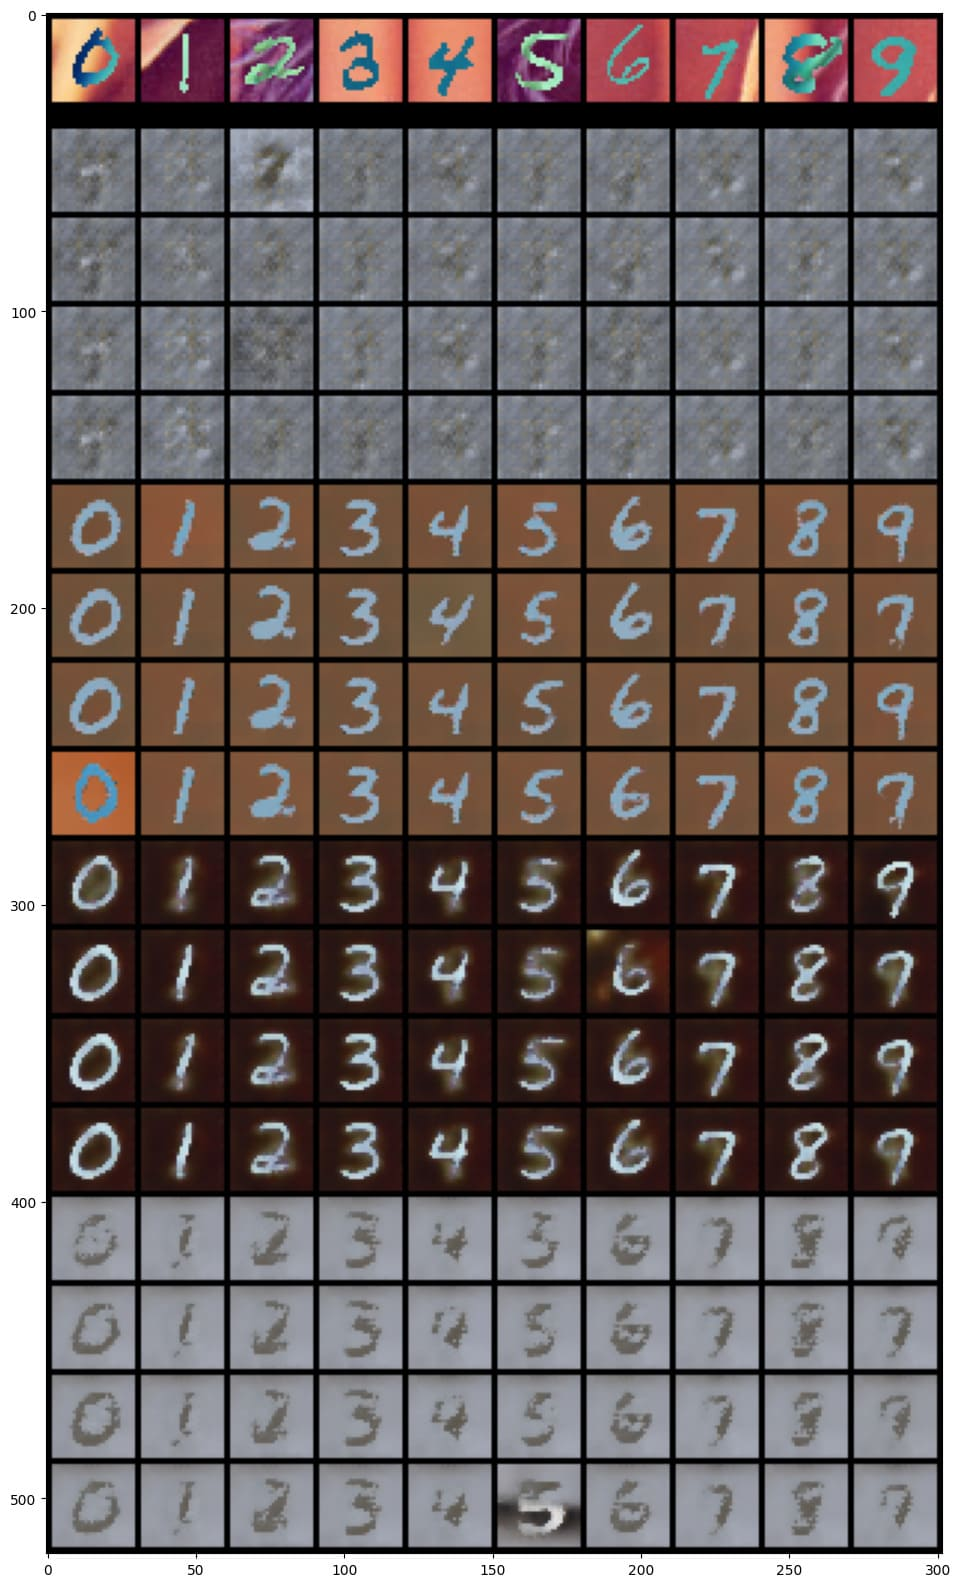
\includegraphics[width=\linewidth]{figures/datasets/mmnist/quali/nexus_cond_m2_out_remaining_mmnist}
         \caption*{\gls{NEXUS}}
      
     \end{subfigure}
     
  \begin{subfigure}{0.2\textwidth}
         \centering
         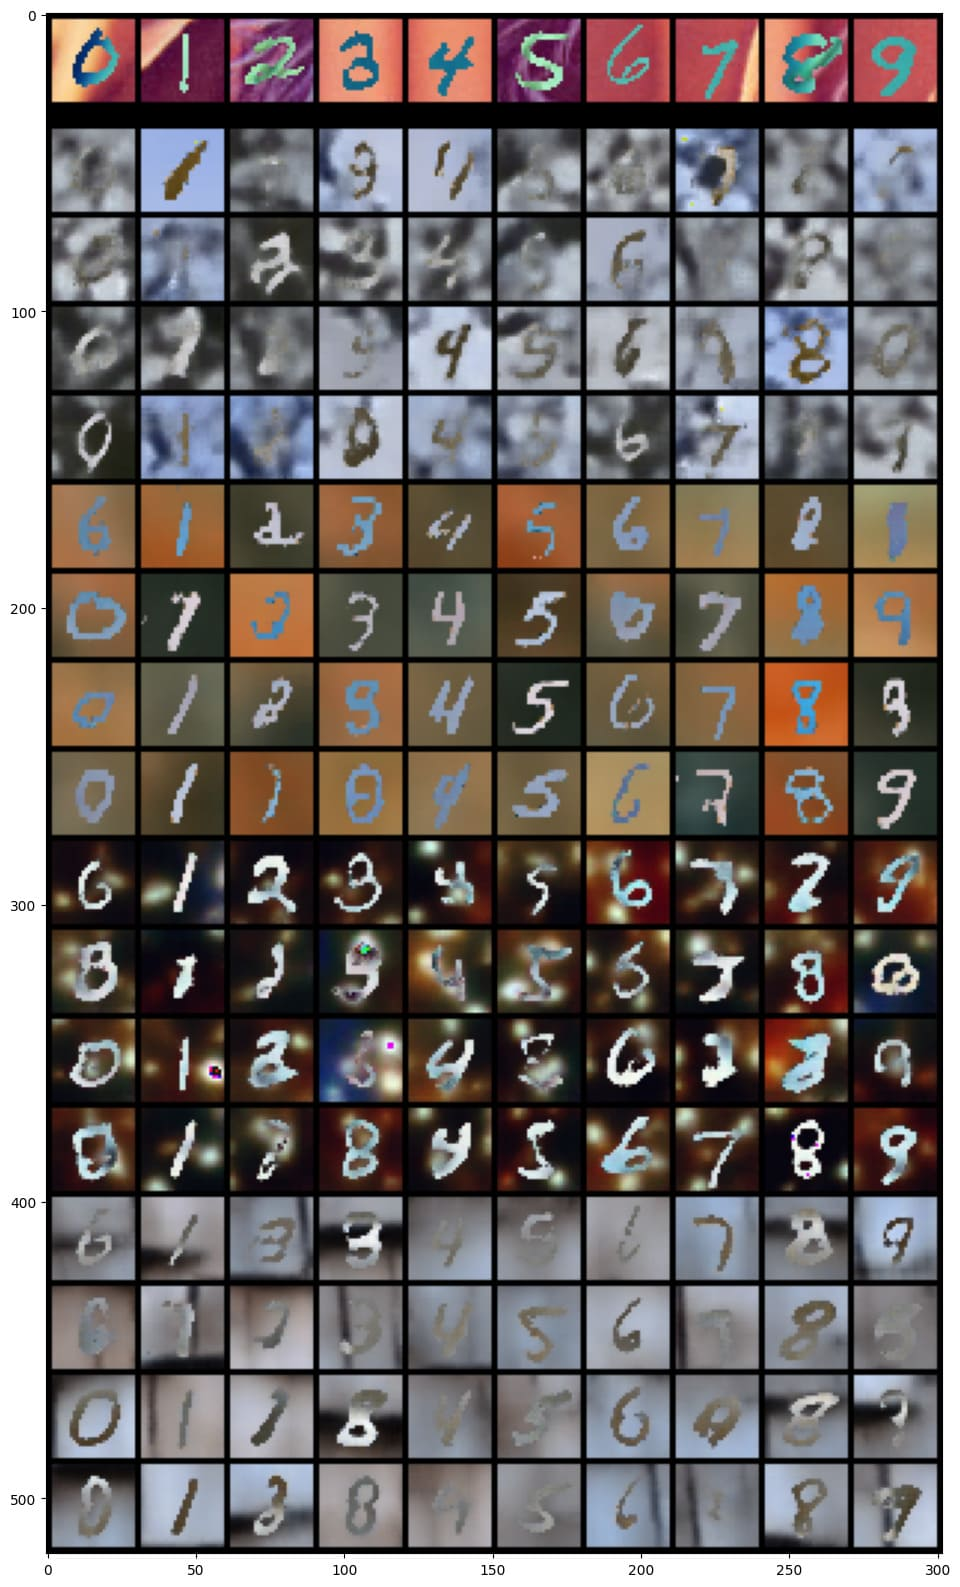
\includegraphics[width=\linewidth]{figures/datasets/mmnist/quali/mvtcae_cond_m2_out_remaining_mmnist}
         \caption*{\gls{MVTCAE}}
     
     \end{subfigure}
    \begin{subfigure}{0.20\textwidth}
         \centering
         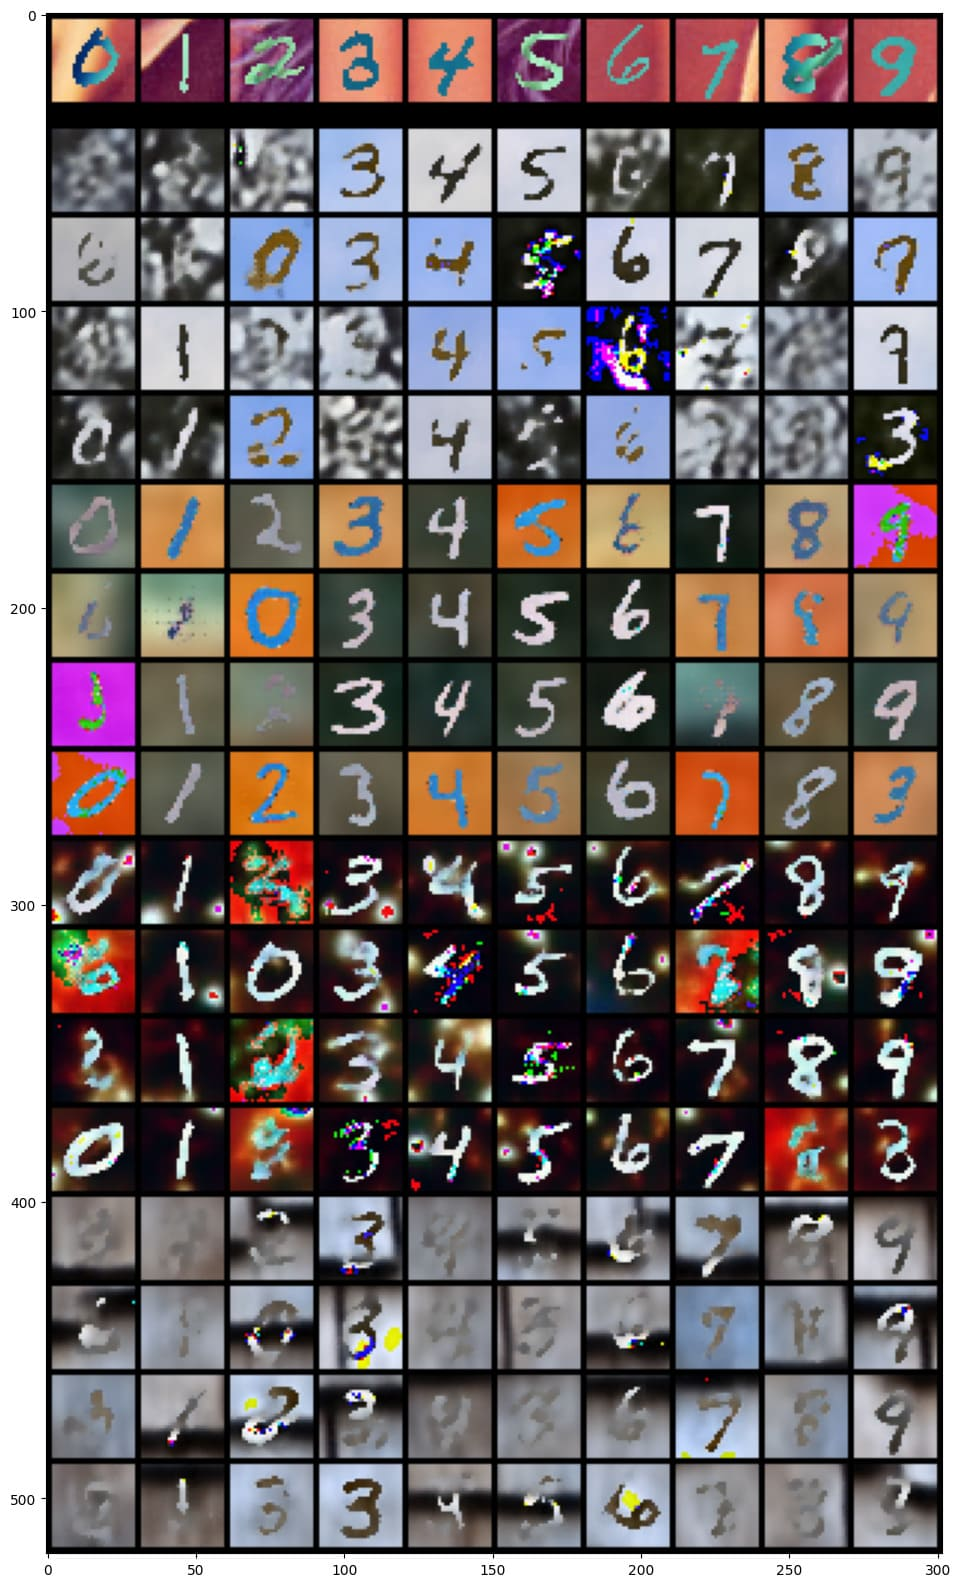
\includegraphics[page=1,width=\linewidth]{figures/datasets/mmnist/quali/MLD_inpaint_cond_m2_out_remaining_mmnist}
         \caption*{\gls{MLD Inpaint} }
    
     \end{subfigure}
  \begin{subfigure}{0.20\textwidth}
         \centering
         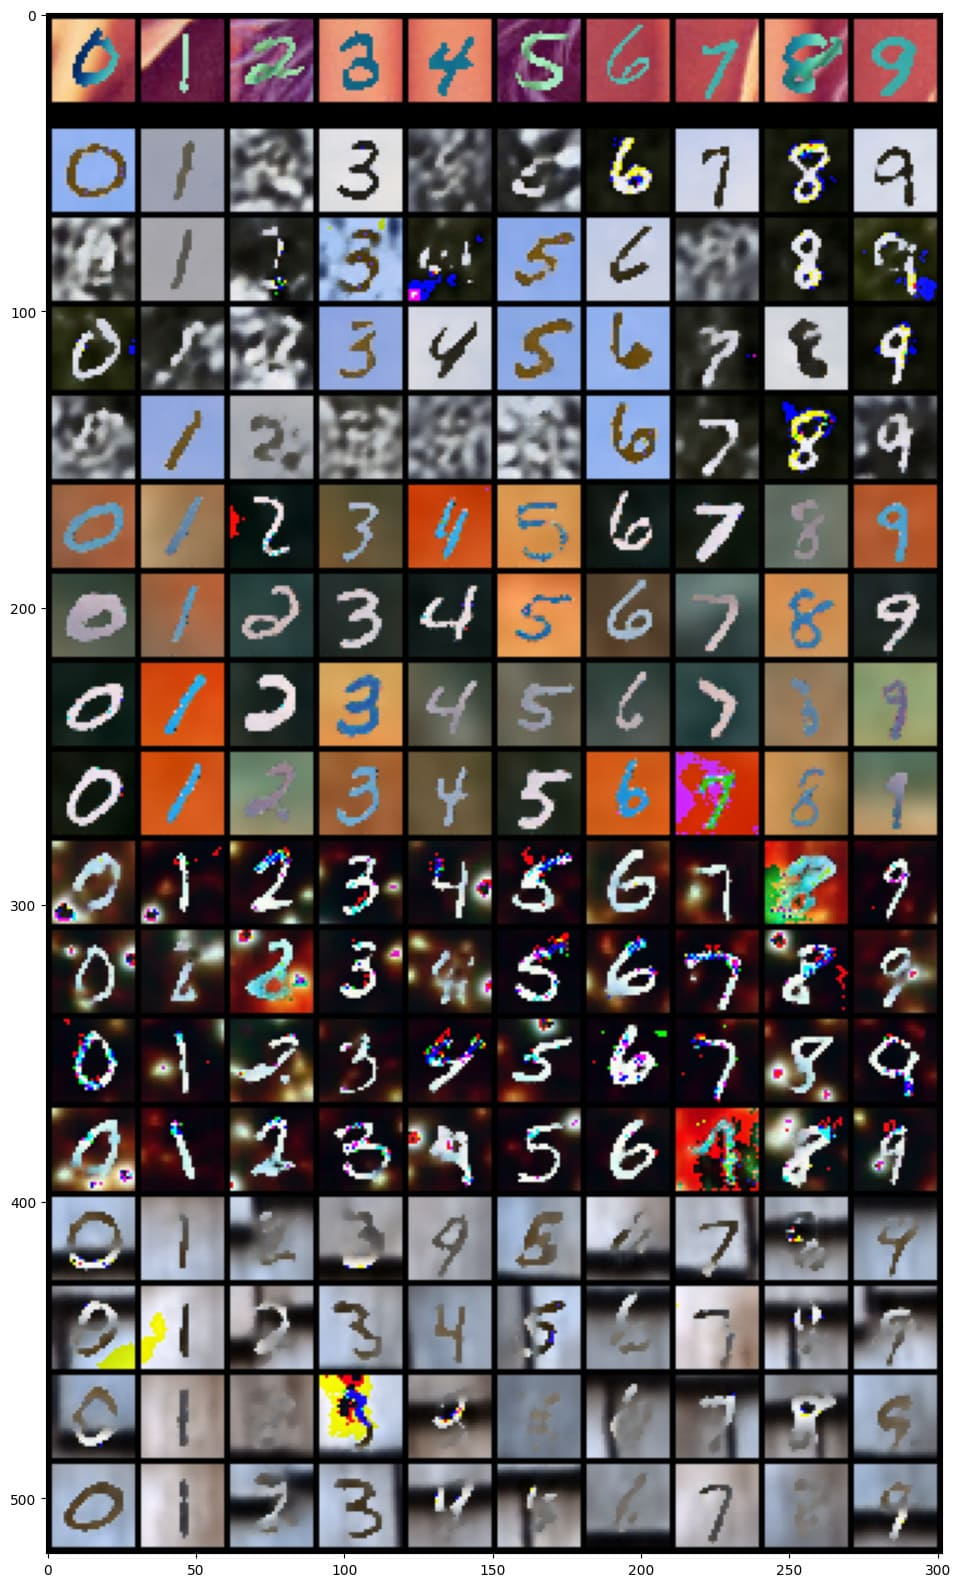
\includegraphics[page=1,width=\linewidth]{figures/datasets/mmnist/quali/MLD_uni_cond_m2_out_remaining_mmnist}
         \caption*{\gls{MLD Uni} }
     
     \end{subfigure}
  \begin{subfigure}{0.20\textwidth}
         \centering
         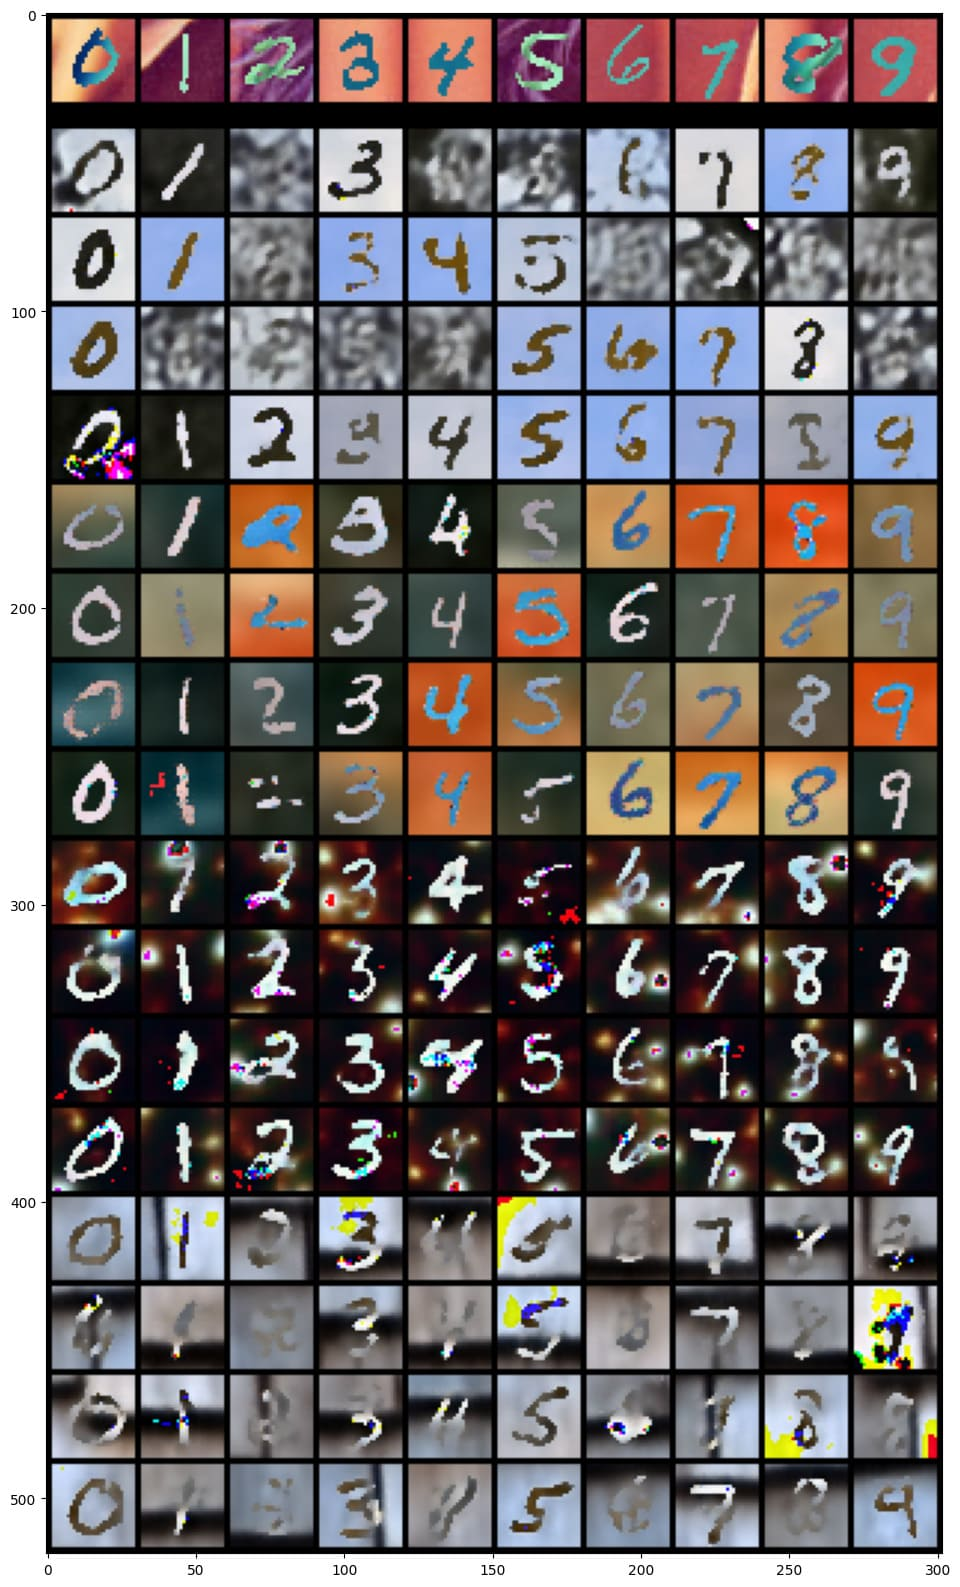
\includegraphics[page=1,width=\linewidth]{figures/datasets/mmnist/quali/MLD_cond_m2_out_remaining_mmnist}
         \caption*{ \textbf{\gls{MLD} (ours)} }

     \end{subfigure}
     
        \caption{Conditional generation qualitative results for \textbf{\polymnist} . The modality $X^2$ (dirst row) is used as the condition to generate the 4 remaining modalities(The rows below).  }
        \label{fig:cond_mmnist_2}
\end{figure}





\begin{figure}[h]
     \centering
       \centering
     \begin{subfigure}{0.2\textwidth}
         \centering
         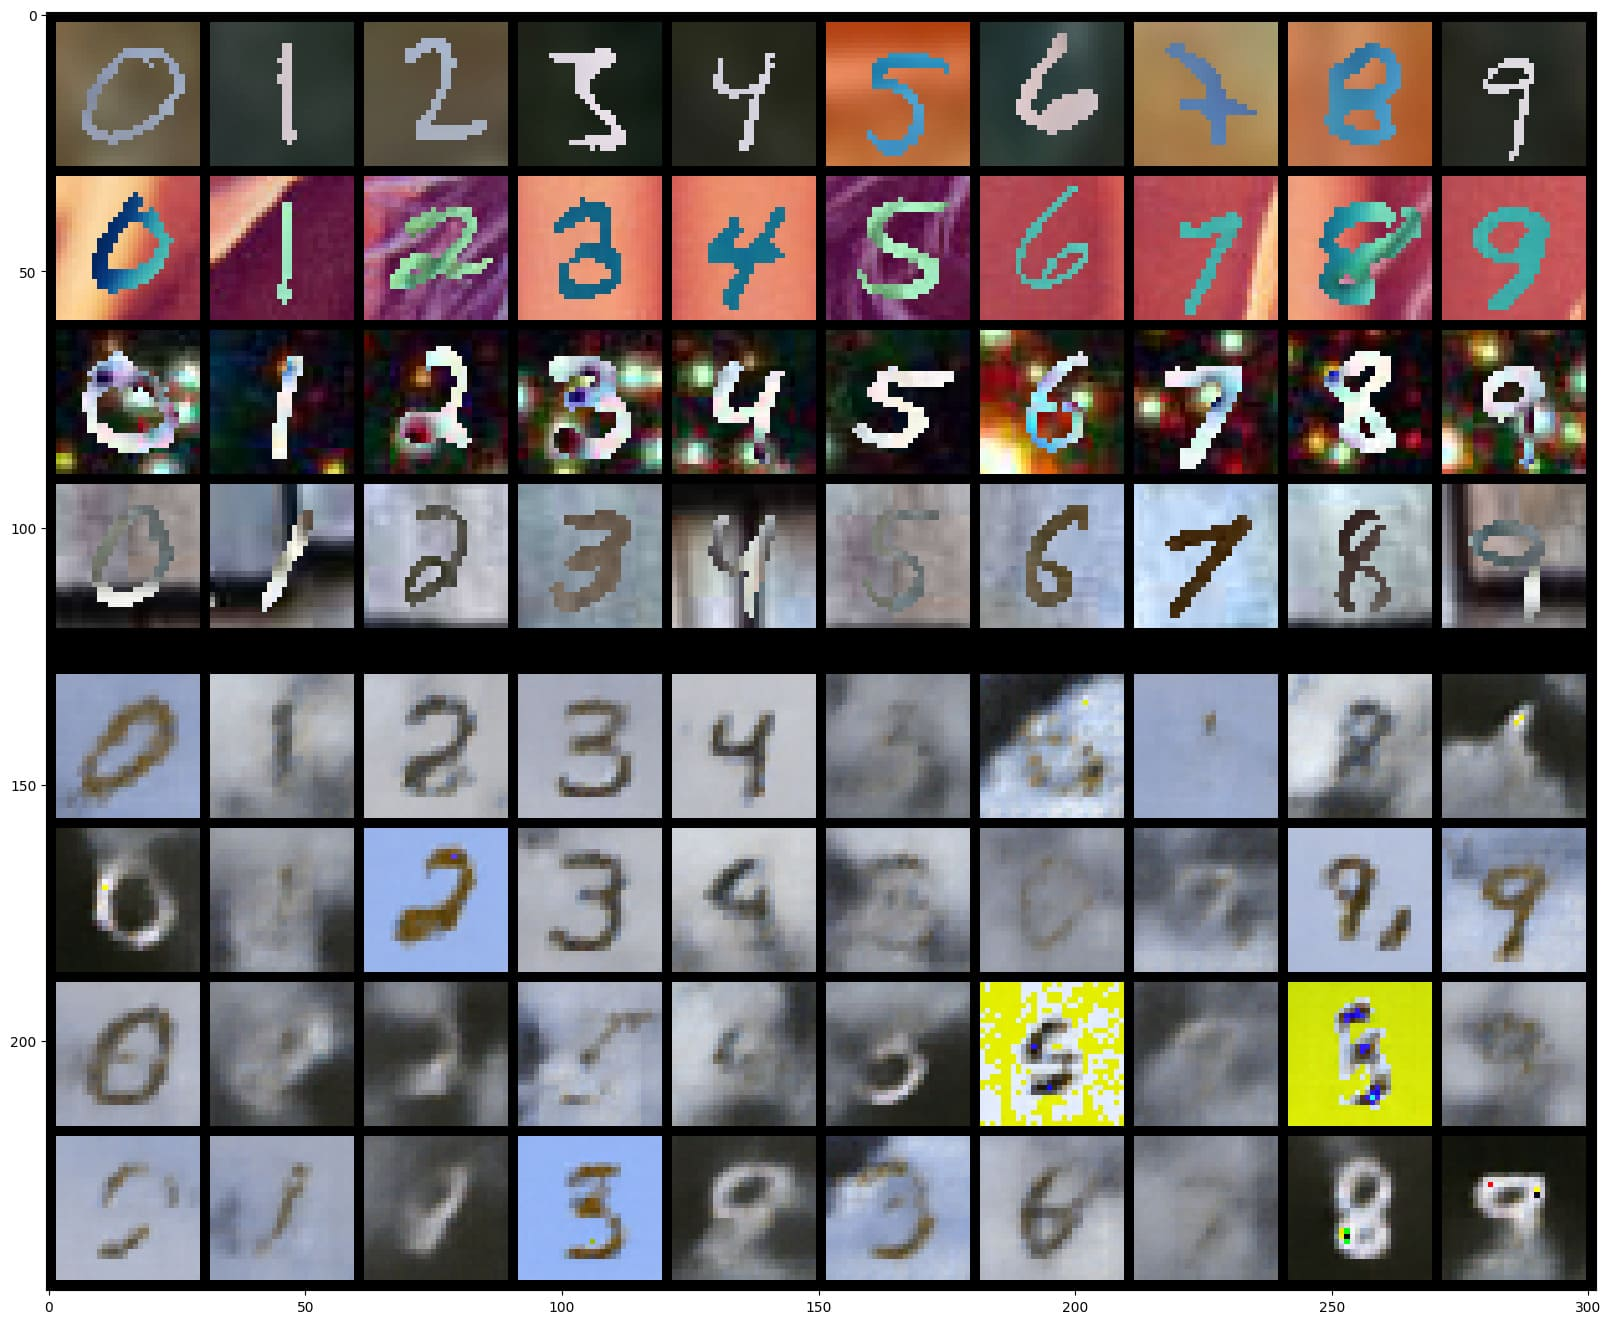
\includegraphics[width=\linewidth]{figures/datasets/mmnist/quali/mvae_cond_m1,m2,m3,m4_out_remaining_mmnist}
         \caption*{\gls{MVAE}}

     \end{subfigure}
     \begin{subfigure}{0.2\textwidth}
         \centering
         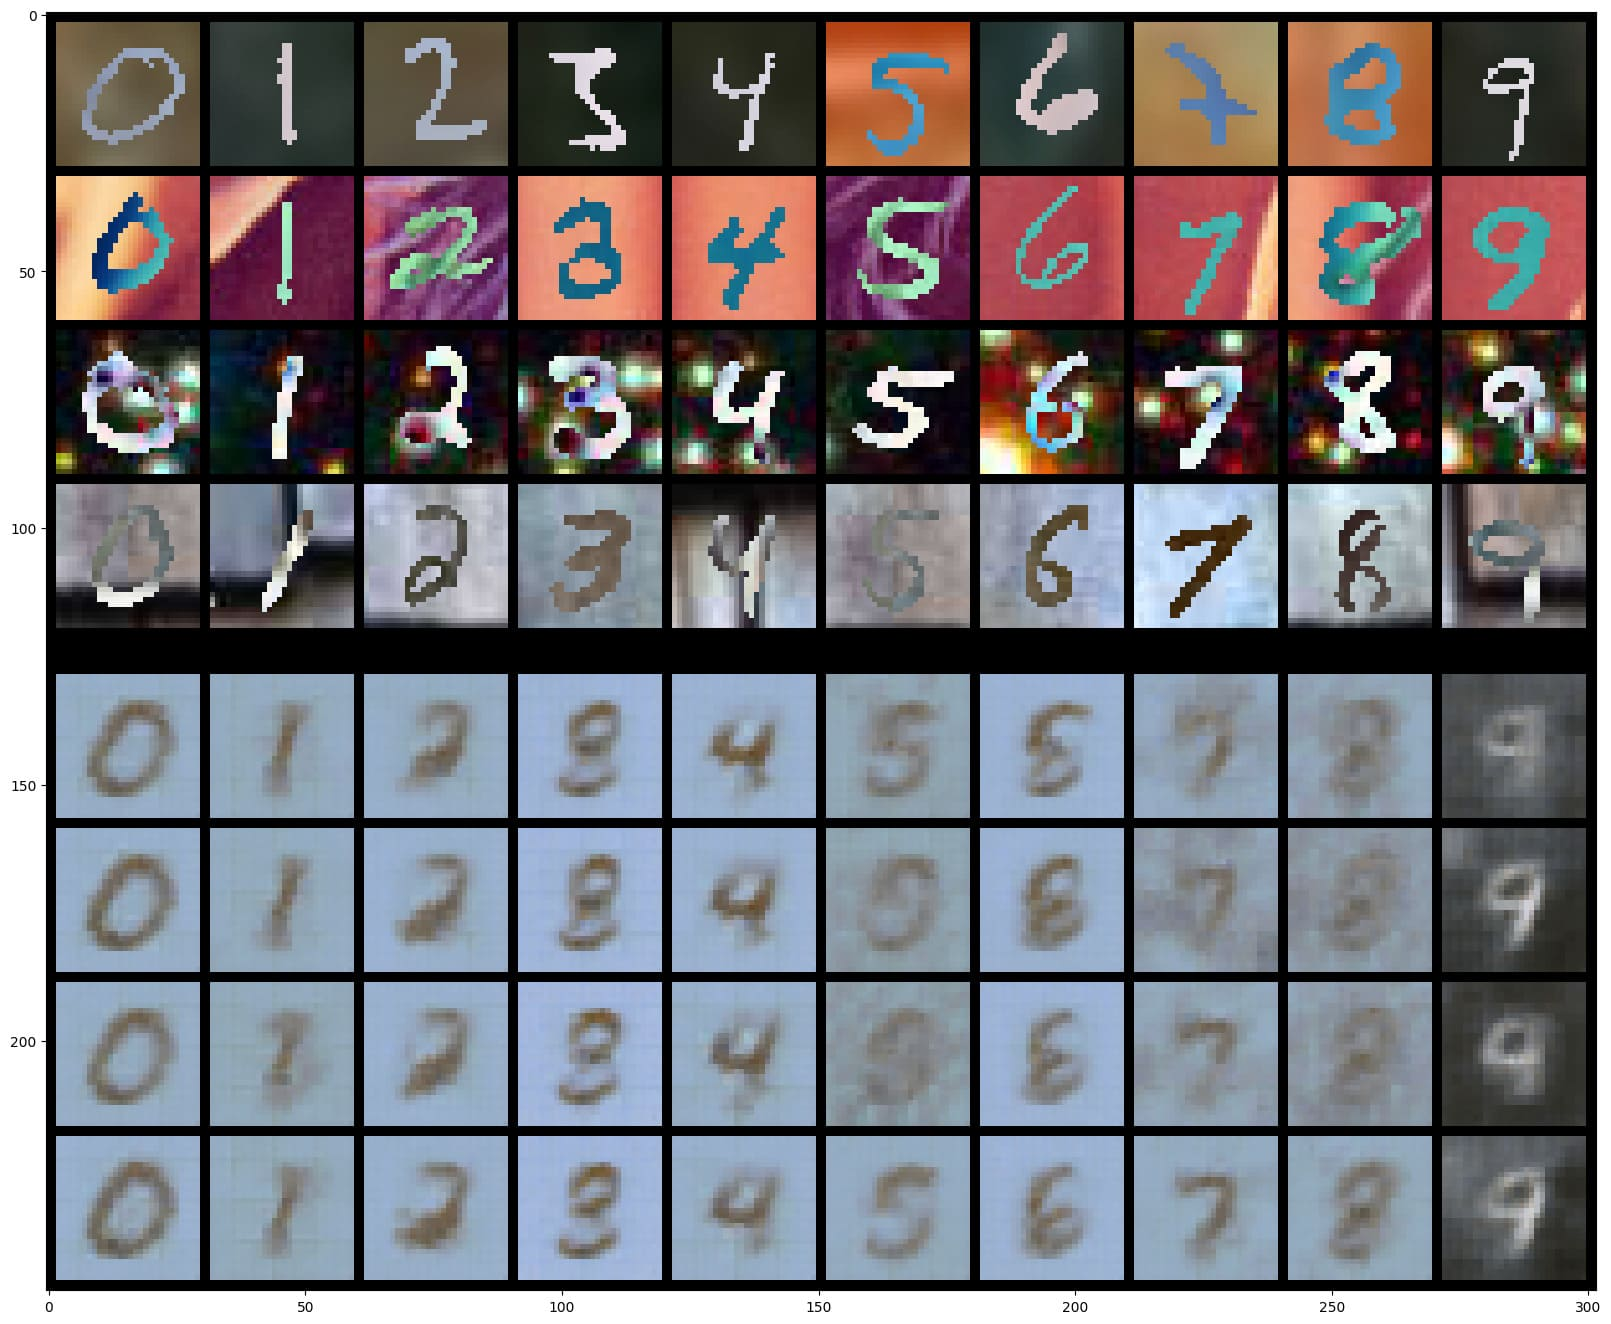
\includegraphics[width=\linewidth]{figures/datasets/mmnist/quali/mmvae_cond_m1,m2,m3,m4_out_remaining_mmnist}
         \caption*{\gls{MMVAE}}

     \end{subfigure}
       \begin{subfigure}{0.2\textwidth}
         \centering
         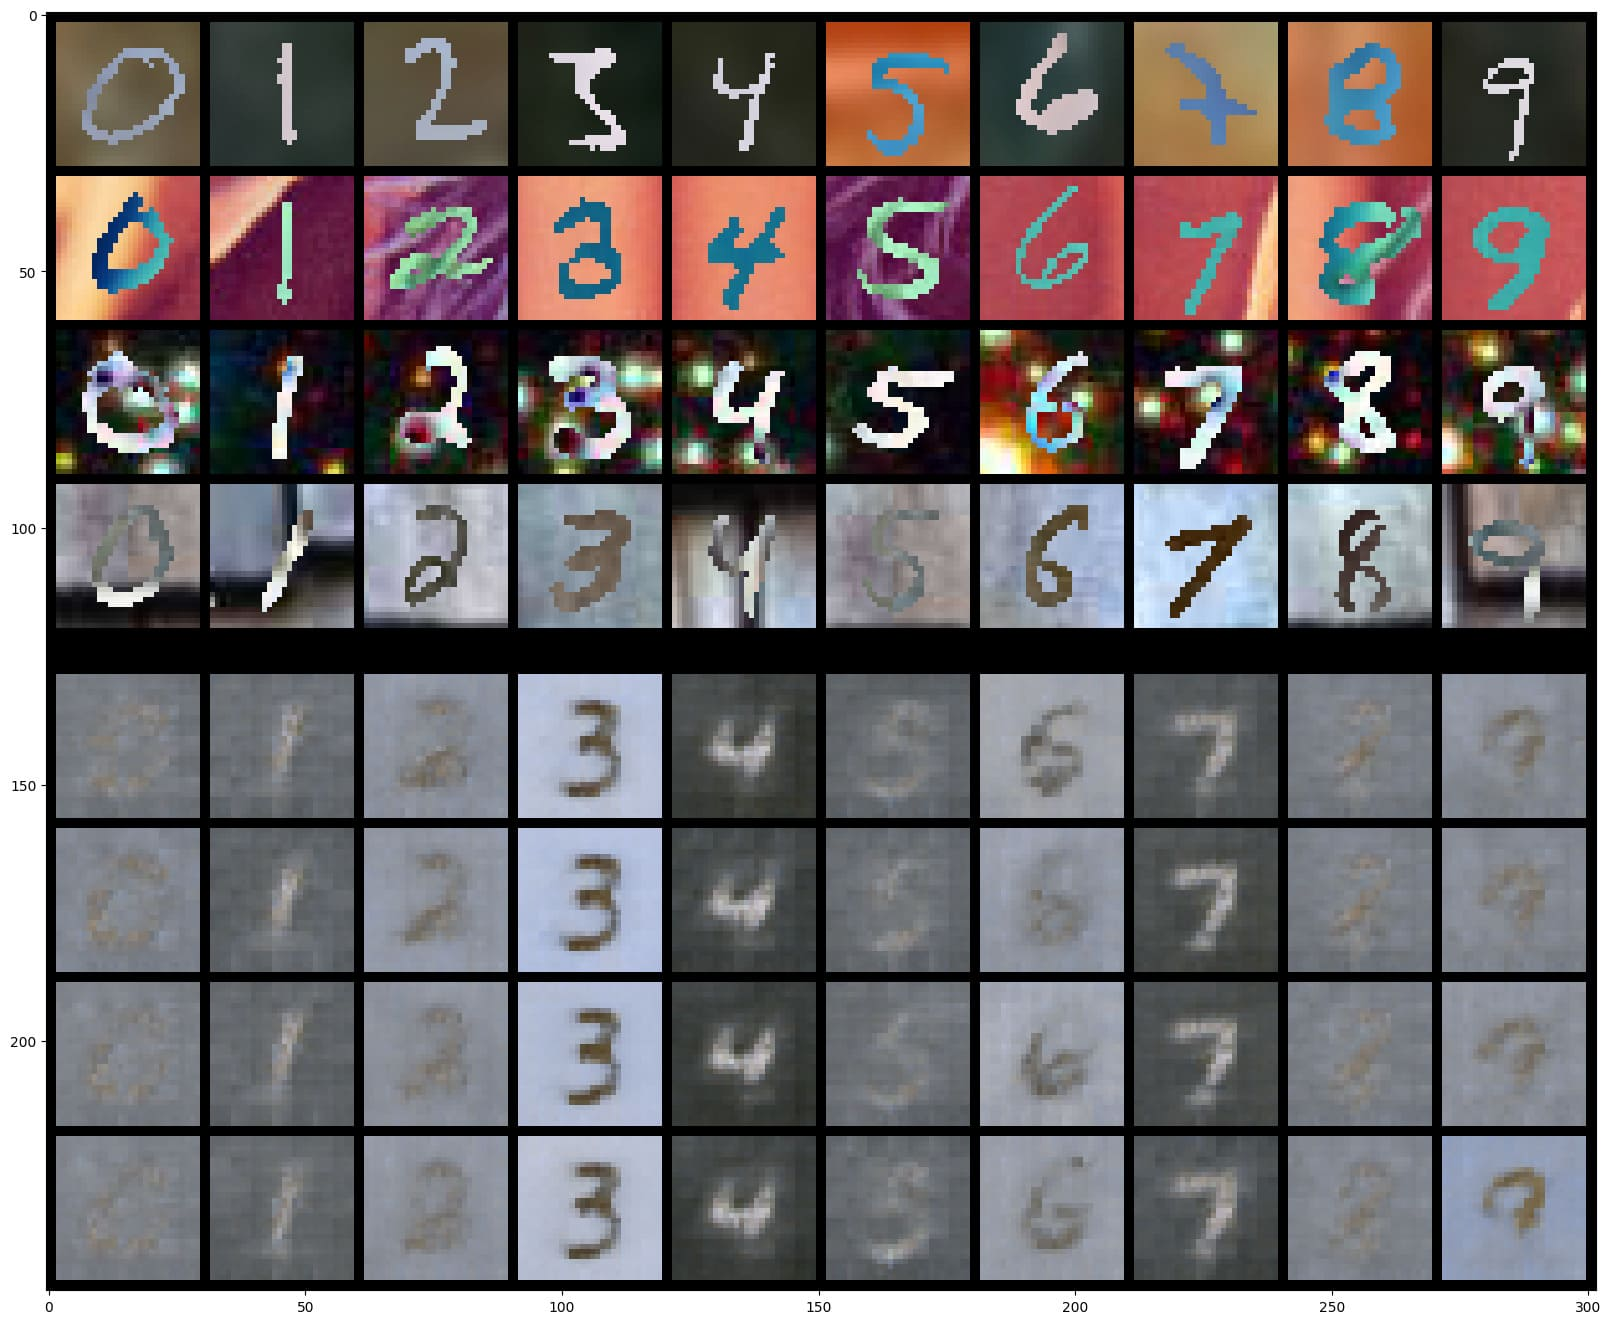
\includegraphics[width=\linewidth]{figures/datasets/mmnist/quali/mopoe_cond_m1,m2,m3,m4_out_remaining_mmnist}
         \caption*{\gls{MOPOE}}
    
     \end{subfigure}
      \begin{subfigure}{0.2\textwidth}
         \centering
         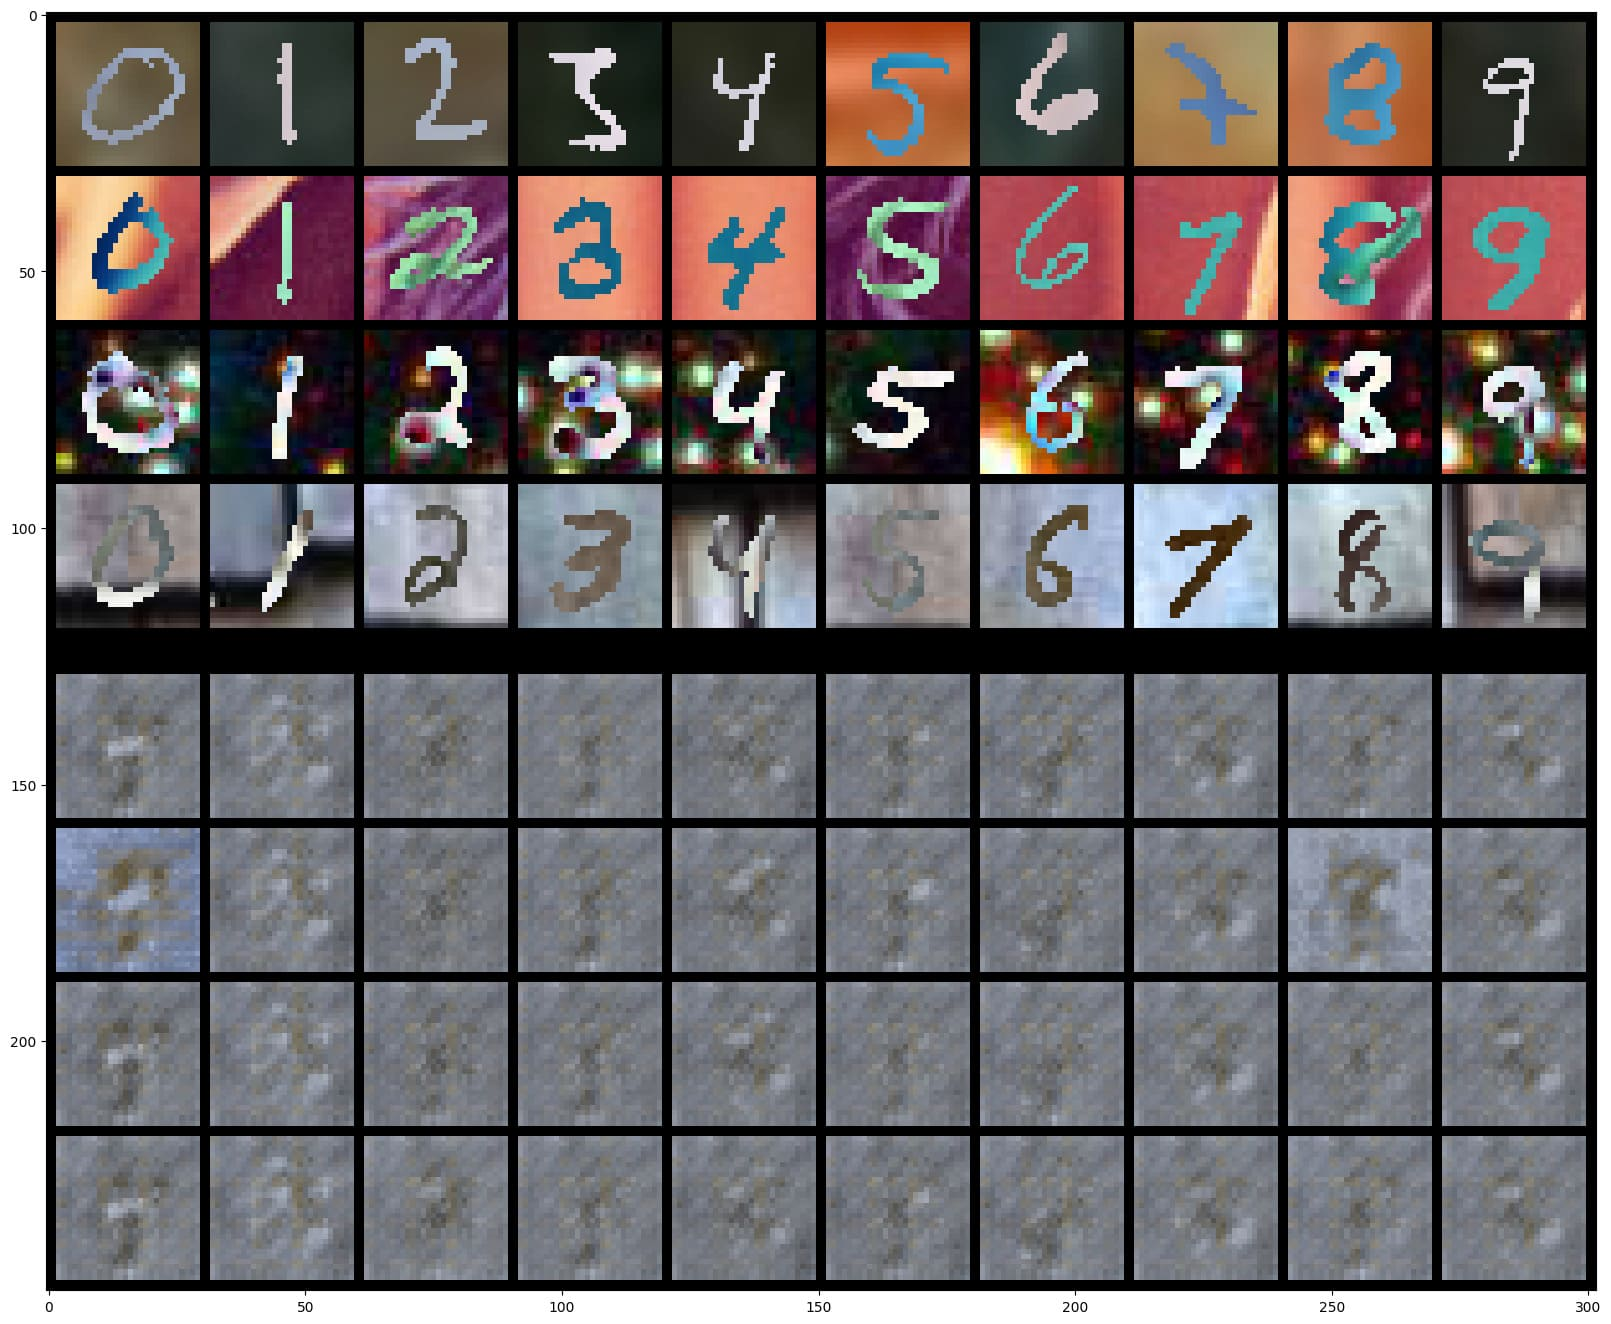
\includegraphics[width=\linewidth]{figures/datasets/mmnist/quali/nexus_cond_m1,m2,m3,m4_out_remaining_mmnist}
         \caption*{\gls{NEXUS}}

     \end{subfigure}
     
  \begin{subfigure}{0.2\textwidth}
         \centering
         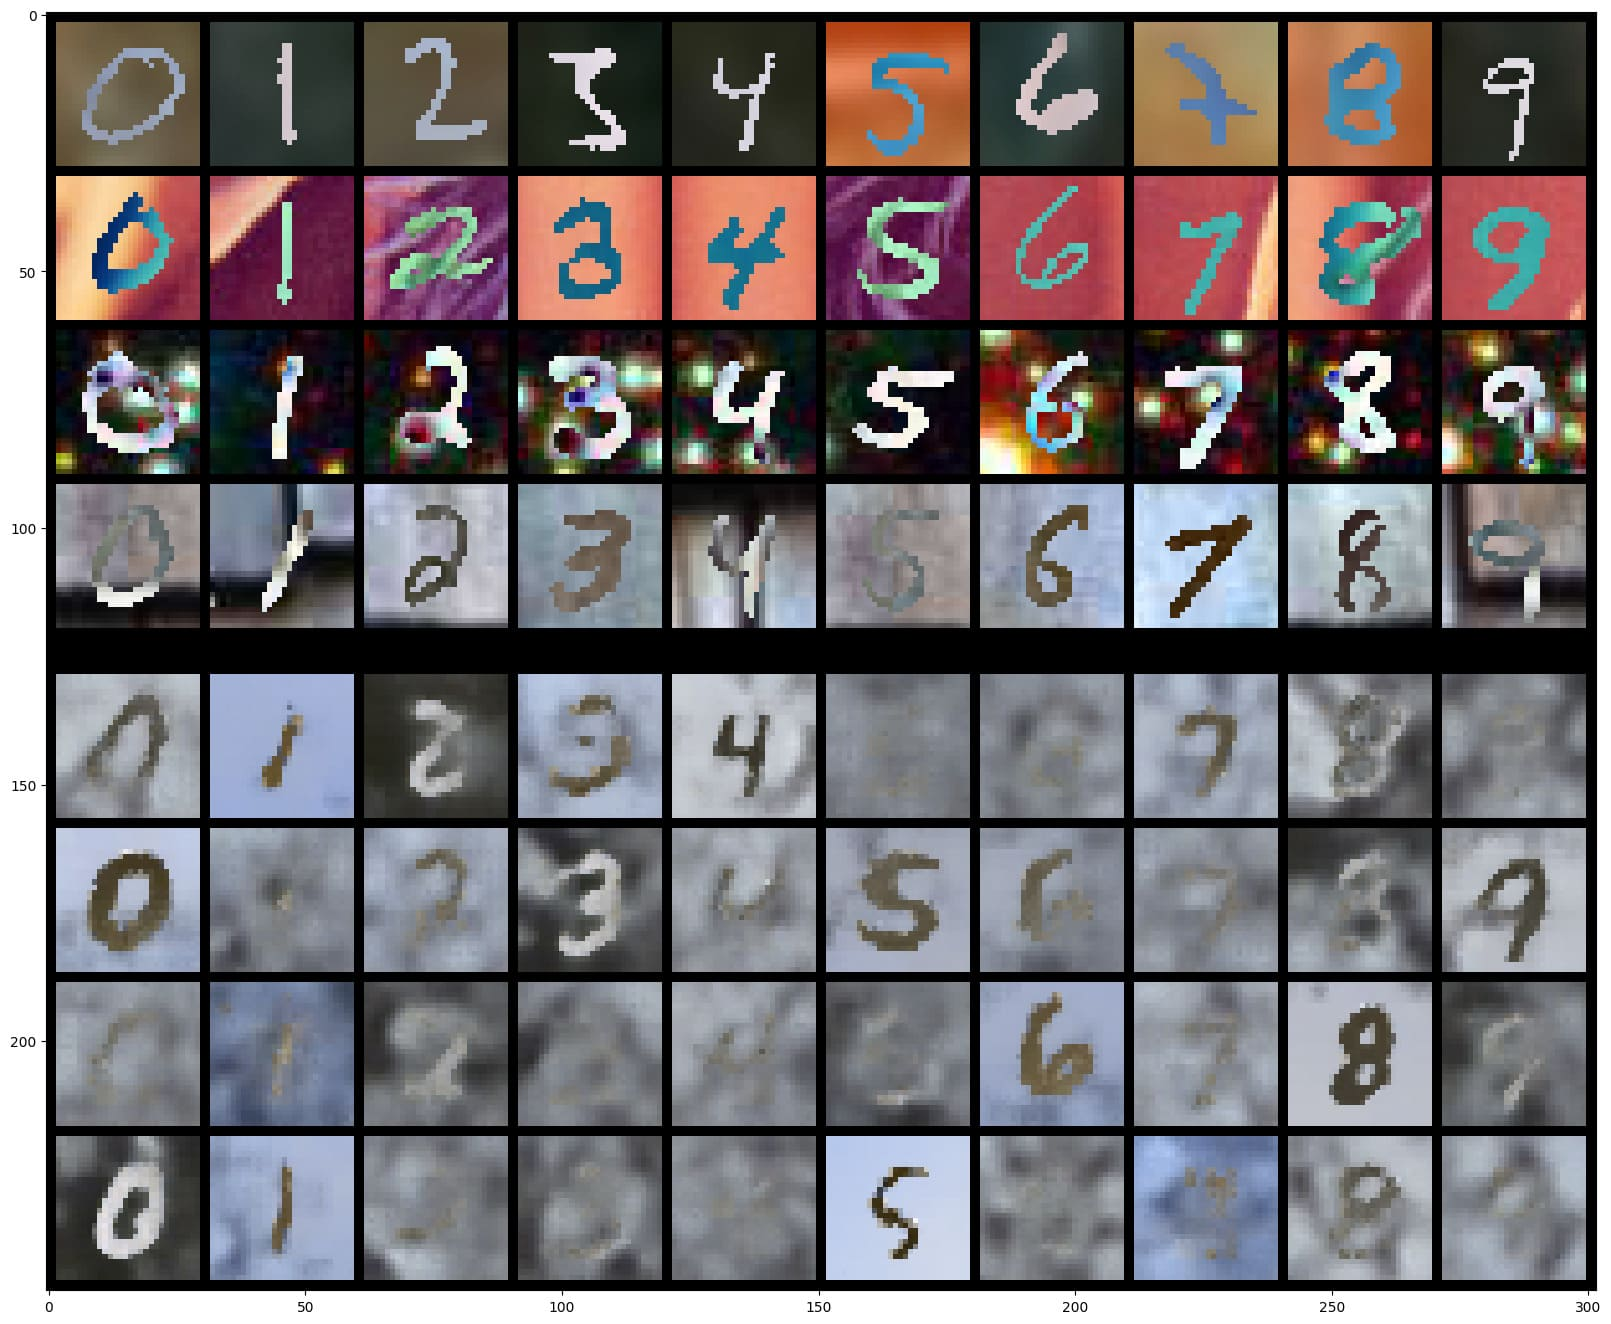
\includegraphics[width=\linewidth]{figures/datasets/mmnist/quali/mvtcae_cond_m1,m2,m3,m4_out_remaining_mmnist}
         \caption*{\gls{MVTCAE}}
 
     \end{subfigure}
    \begin{subfigure}{0.2\textwidth}
         \centering
         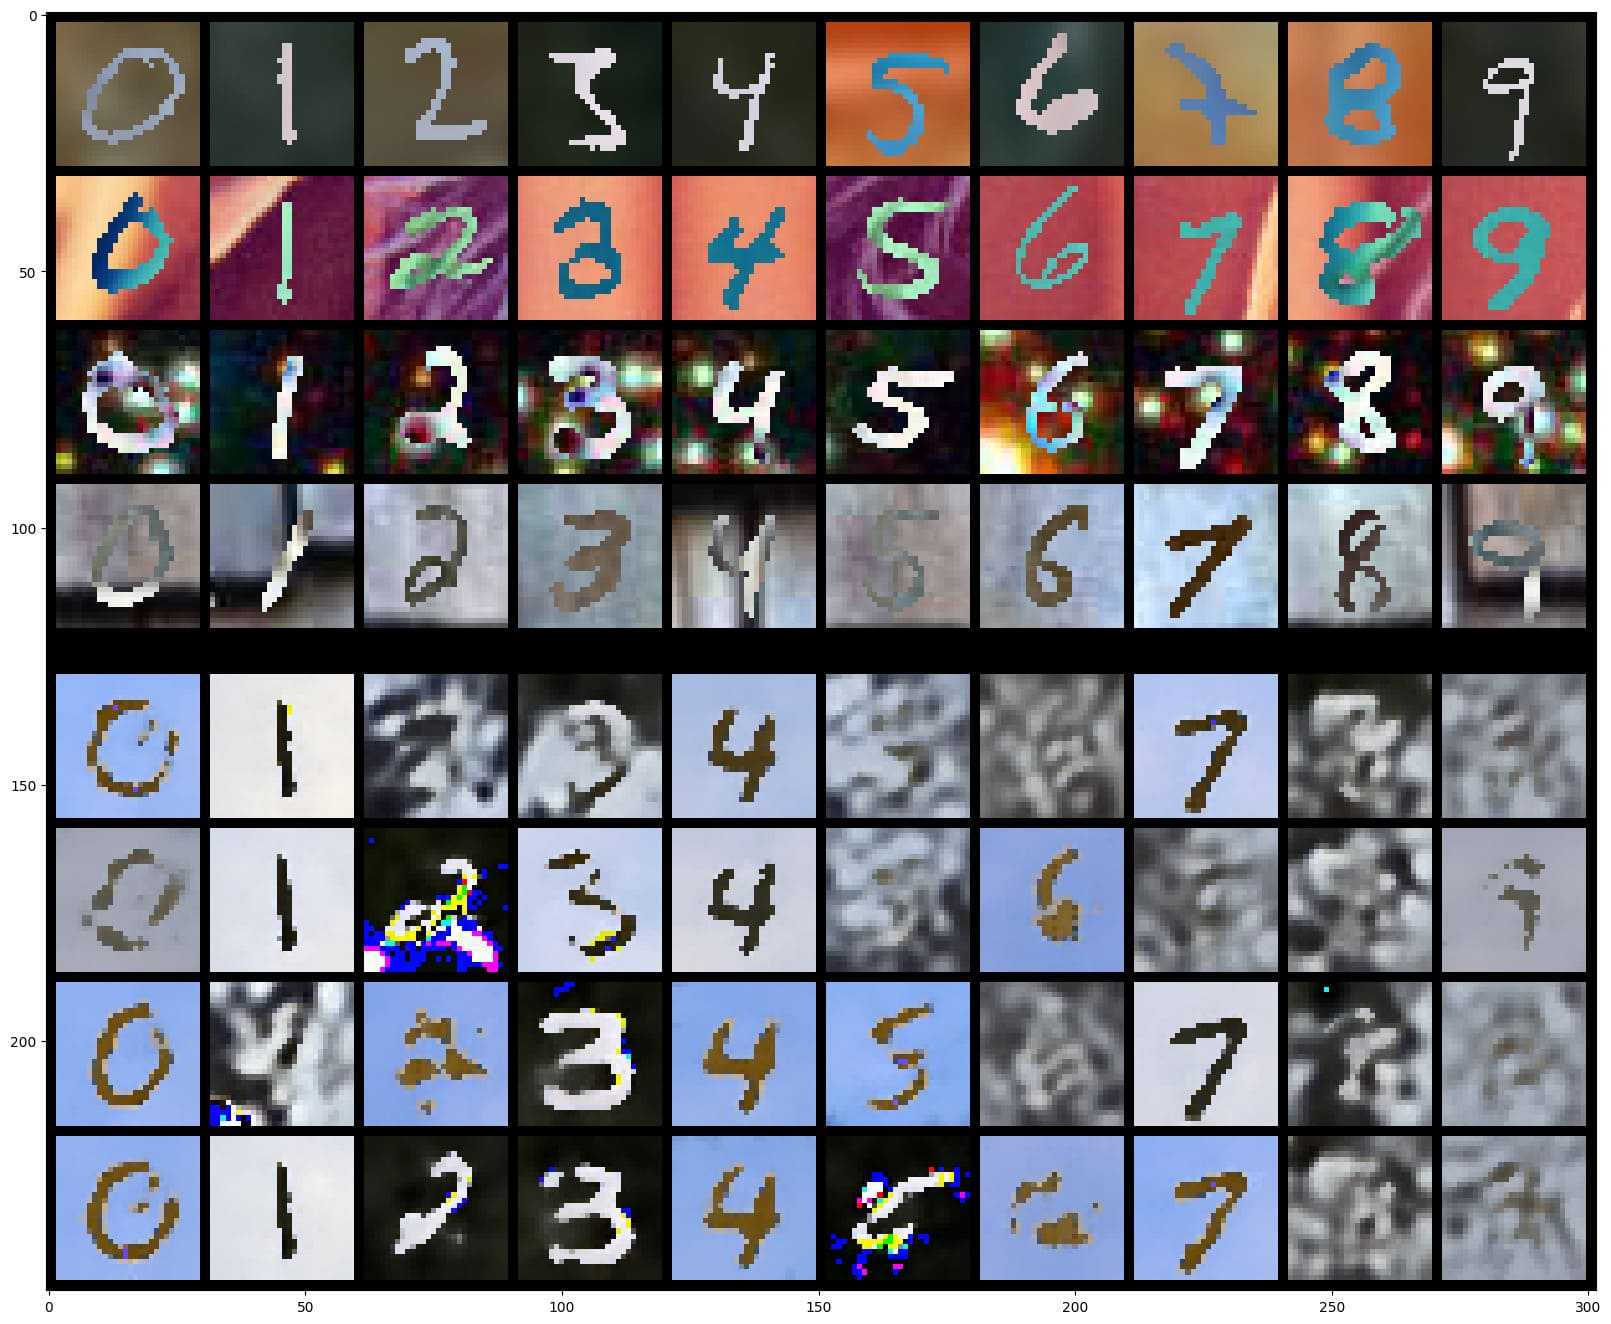
\includegraphics[page=1,width=\linewidth]{figures/datasets/mmnist/quali/MLD_inpaint_cond_m1,m2,m3,m4_out_remaining_mmnist}
         \caption*{\gls{MLD Inpaint}  }
     \end{subfigure}
  \begin{subfigure}{0.2\textwidth}
         \centering
         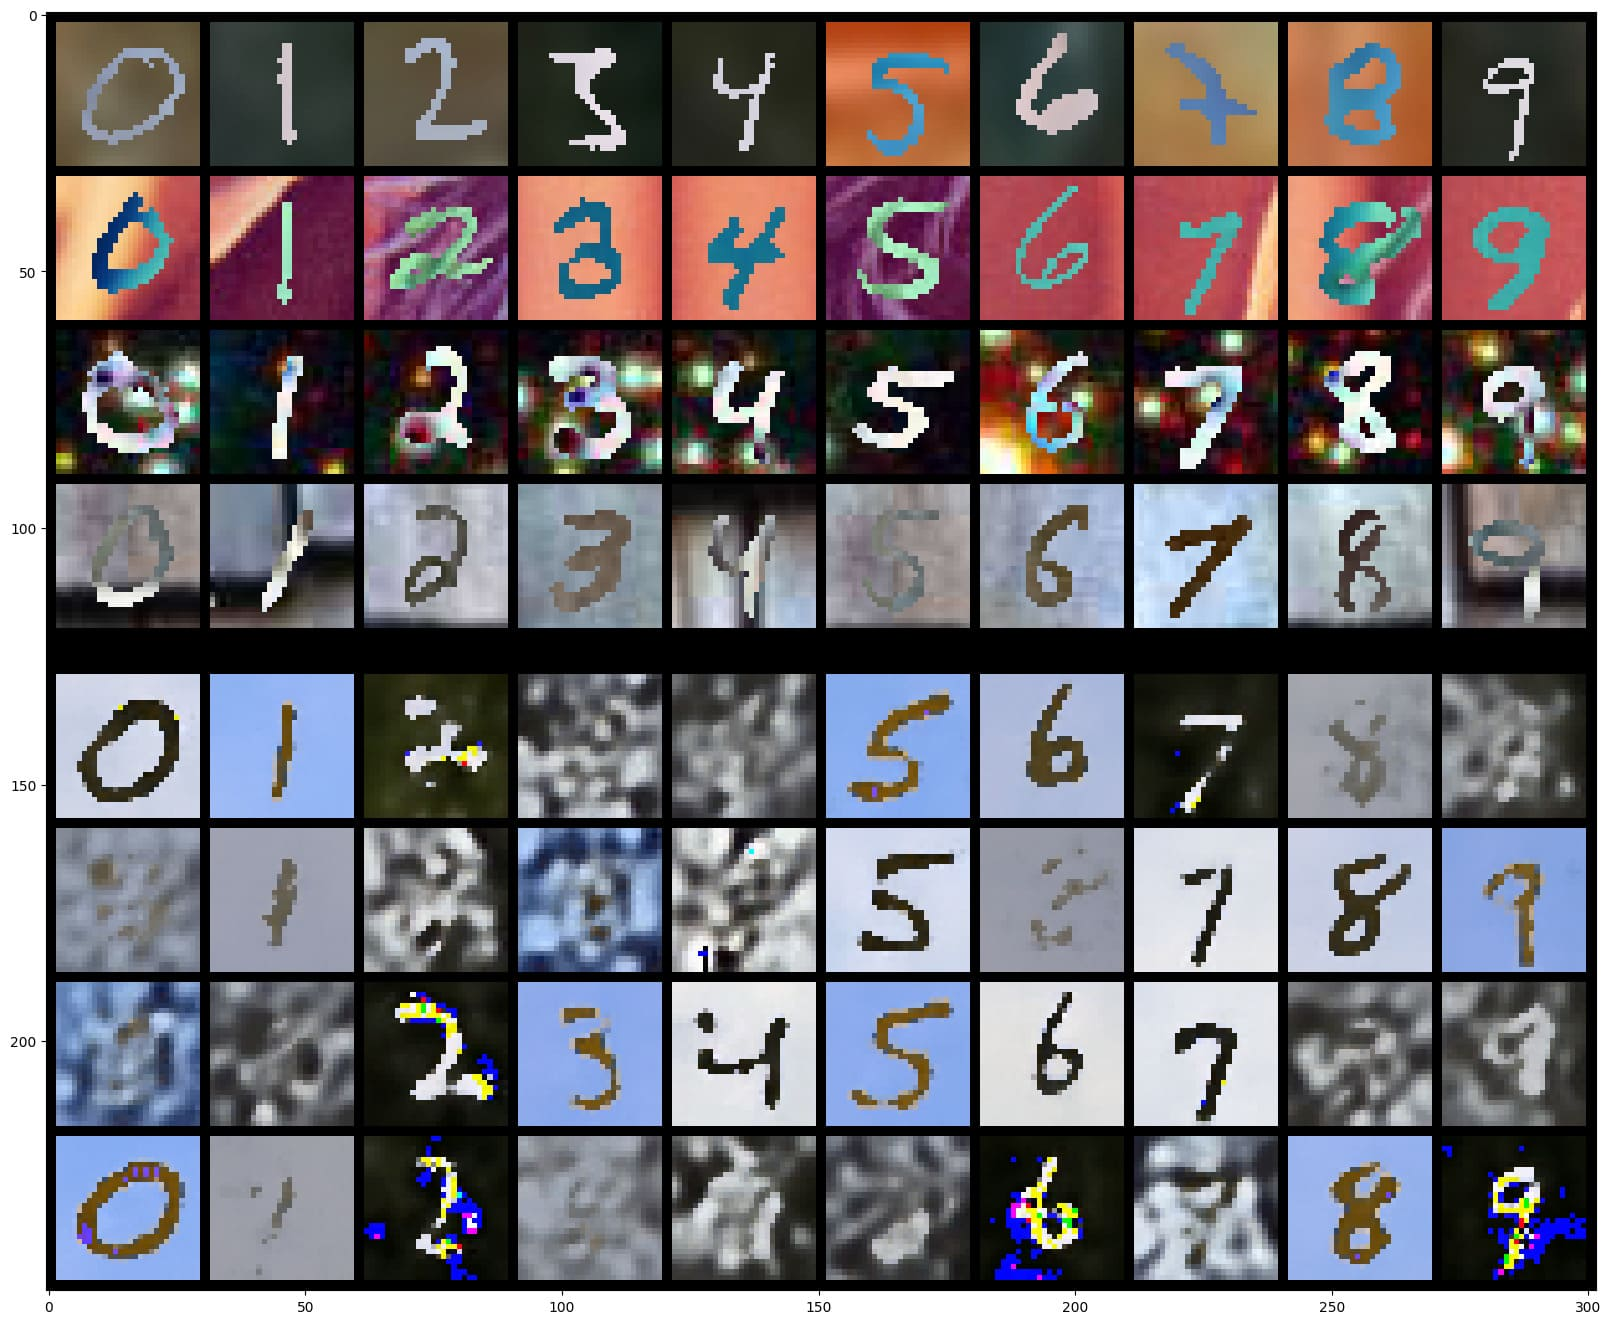
\includegraphics[page=1,width=\linewidth]{figures/datasets/mmnist/quali/MLD_uni_cond_m1,m2,m3,m4_out_remaining_mmnist}
         \caption*{\gls{MLD Uni}}
     \end{subfigure}
  \begin{subfigure}{0.2\textwidth}
         \centering
         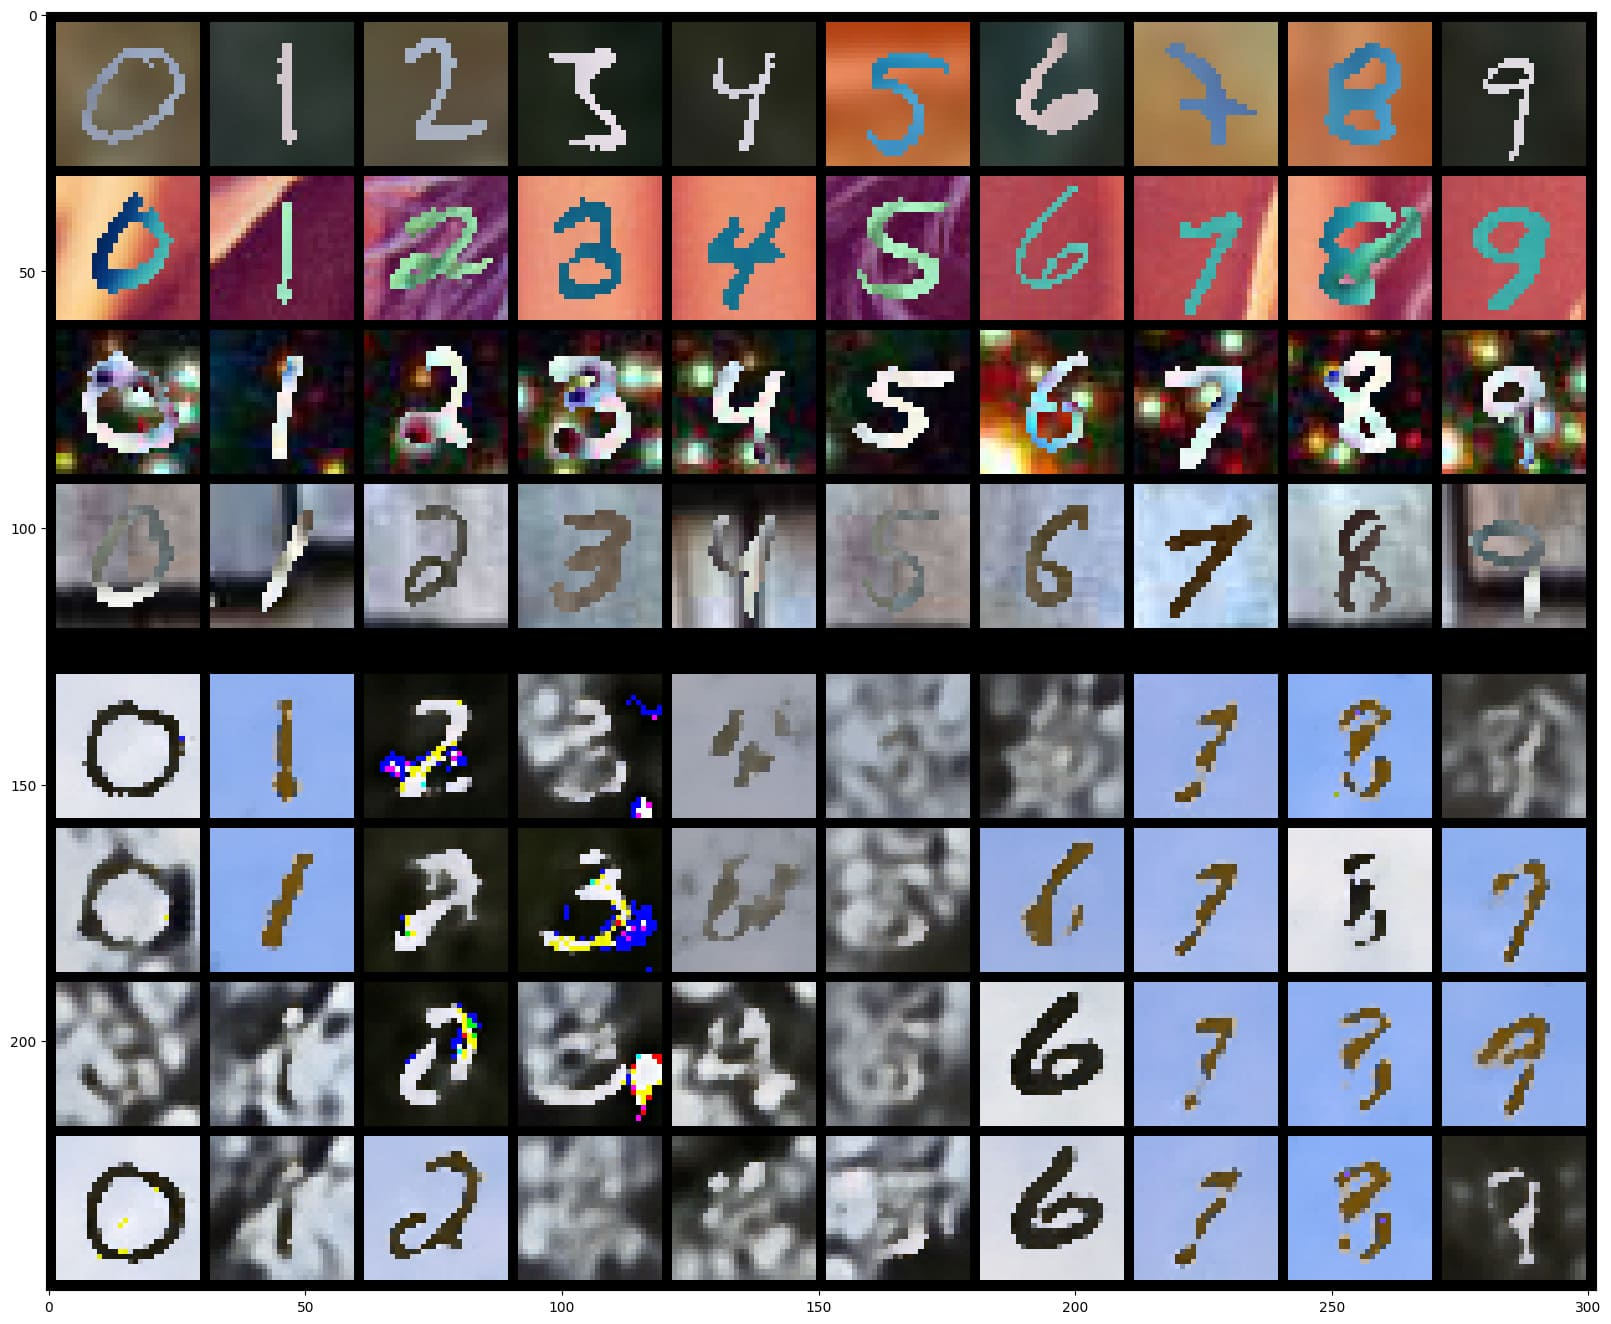
\includegraphics[page=1,width=\linewidth]{figures/datasets/mmnist/quali/MLD_cond_m1,m2,m3,m4_out_remaining_mmnist}
         \caption*{\textbf{\gls{MLD} (ours)}}
     \end{subfigure}
        \caption{Conditional generation qualitative results for \textbf{\polymnist}. The subset of modalities $X^1 ,X^2,X^3,X^4 $ (First 4 rows) are used as the condition to generate the modality $X^0$ (The rows below).  }
        \label{fig:cond_mmnist_1234}
\end{figure}
\newpage


\subsubsection{Additional experiments with \cite{palumbo2023mmvae} architecture}

In our experiments on \polymnist, we used the same architecture as in \cite{sutter2021generalized} \cite{tcmvaehwang21} to ensure a fair settings for all the baselines. In \cite{palumbo2023mmvae}, the experiments on \polymnist are conducted using a different autoencoder architecture which is based on Resnets instead of a a sequence of convolutions layers based autoencoder. We investigate in this section, the performance of \gls{MMVAEplus} and our \gls{MLD} using this architecture. For \gls{MMVAEplus}, we keep the same settings as in \cite{palumbo2023mmvae} including the autoencoder architecture, latent size, and importance sampling K=10 with doubly reparameterized gradient estimator (DReG). For \gls{MLD}, we use the same autoencoder architecture with latent size equal to 160. In \Cref{fig:mmvaeresnet}, we observe that while the new architecture autoencoder enhance the \gls{MMVAEplus} performance, our \gls{MLD} performance is improved as well. Similarly to previous results, \gls{MLD} achieves simultaneously the best generative coherence and quality.



\begin{figure} [H]  
\centering
\begin{subfigure}{0.30\textwidth}
    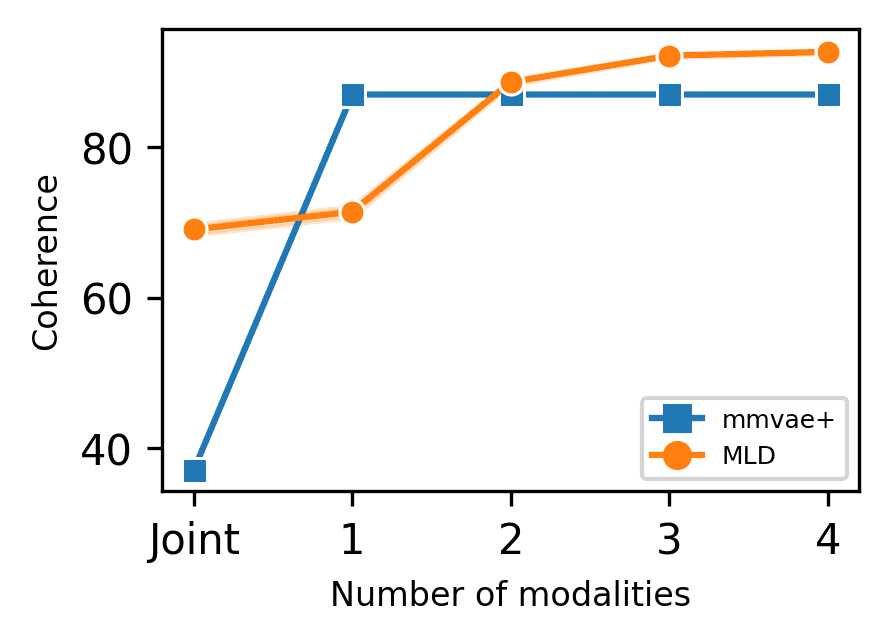
\includegraphics[width=\linewidth]{figures/datasets/mmnist/quant/mmvaeplus_mmnist_plot_coh_avg.png}
\end{subfigure}
\begin{subfigure}{0.30\textwidth}
    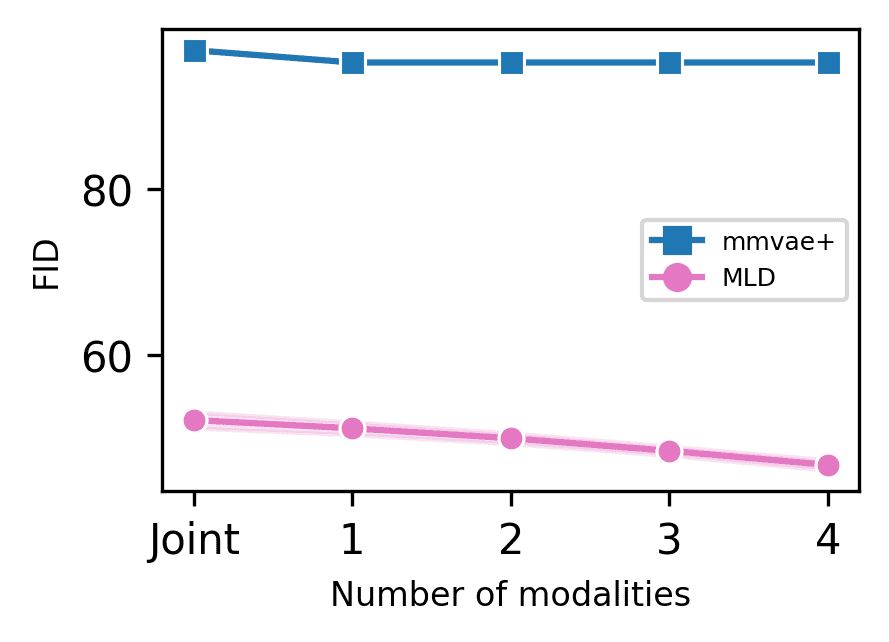
\includegraphics[width=\linewidth]{figures/datasets/mmnist/quant/mmvaeplus_mmnist_plot_fid_avg.png}
\end{subfigure}

\label{fig:mmvaeresnet}  
\caption{Results for POLYMNIST data-set. Left: a comparison of the generative coherence (
 $ \uparrow $ ) and quality in terms of FID ($ \downarrow $) as a function of the number of inputs.}
\end{figure}


\subsection{CUB}

\begin{table}[H]
\tiny
\centering
\begin{tabular}{c|c|cc|cc}
\toprule
\multirow{2}{*}{ Models }  & \multicolumn{3}{c}{ Coherence ( $ \uparrow $ ) }  &  \multicolumn{2}{c}{Quality ( $ \downarrow $ ) }  \\
    \cmidrule{2-6}
    &  Joint &Image $\rightarrow$ Caption &  Caption $\rightarrow$ Image & Joint $\rightarrow$ Image & Caption $\rightarrow$ Image \\
    \midrule
    
    \gls{MVAE} & $0.66$&$\textbf{0.70}$ &$0.64$ & 
    $158.91$ &  $158.88$
\\
  \gls{MMVAE} & $0.66$&$0.69$ &$0.62$ & 
    $277.8$ &  $212.57$   \\
    \gls{MOPOE} & $0.64$&$0.68$ &$0.55$ & 
    $279.78$ &  $179.04$ \\
    
   \gls{NEXUS} & $0.65$&$0.69$ &$0.59$ & 
    $147.96$ &  $262.9$ \\ 
 

   \gls{MVTCAE} &$0.65$&$\textbf{0.70}$ &$0.65$ & 
    $155.75$ &  $168.17$ \\
     \gls{MMVAEplus} &$0.61$&$0.68$ &$0.65$ & 
    $188.63$ &  $247.44$
    \\

     \gls{MMVAEplus}(K=10) &  $0.63$&$0.68$ &$0.62$ & 
    $172.21$ &  $178.88$  
   \\
    \midrule
   \gls{MLD Inpaint} & $\textbf{0.69}$&${0.69}$ &${0.68}$ & 
    ${69.16}$ &  ${68.33}$
    \\
  \gls{MLD Uni}  &$ \textbf{0.69}$&${0.69}$ &$\textbf{0.69}$ & 
    $64.09$ &  $\textbf{61.92}$ \\

    \gls{MLD}  &$ \textbf{0.69}$&$0.69$ &$\textbf{0.69}$ & 
    $\textbf{63.47}$ &  $62.62$ \\
 \midrule
 \gls{MLD}*  &$ \textbf{0.70}$&
 $0.69$ &
 $\textbf{0.69}$ & 
    $\textbf{22.19}$ & 
    $\textbf{22.50}$ \\
 
    \bottomrule

\end{tabular}
\caption{Generation Coherence (\gls{CLIP-S}  : Higher is better ) and Quality (\gls{FID} $\downarrow$ Lower is better ) for CUB dataset. \textbf{\gls{MLD}*} denotes the version of our method using a more powerful image autoencoder.}
\label{coh_qua:cub}

 \end{table}

% \begin{table}[H]
% \tiny
% \centering
% \begin{tabular}{c|c|cc|cc}
% \toprule
% \multirow{2}{*}{ Models }  & \multicolumn{3}{c}{ Coherence ( $ \uparrow $ ) }  &  \multicolumn{2}{c}{Quality ( $ \downarrow $ ) }  \\
%     \cmidrule{2-6}
%     &  Joint &Image $\rightarrow$ Caption &  Caption $\rightarrow$ Image & Joint $\rightarrow$ Image & Caption $\rightarrow$ Image \\
%     \midrule
    
%     \gls{MVAE} & $0.66_{ \pm 0.00 }$&$\textbf{0.70}_{ \pm 0.00 }$ &$0.64_{ \pm 0.00 }$ & 
%     $158.91_{ \pm 1.71 }$ &  $158.88_{ \pm 1.78 }$
% \\
%   \gls{MMVAE} & $0.66_{ \pm 0.01 }$&$0.69_{ \pm 0.00 }$ &$0.62_
% { \pm 0.00 }$ & 
%     $277.8_{ \pm 5.111 }$ &  $212.57_{ \pm 12.1 }$   \\
%     \gls{MOPOE} & $0.64_{ \pm 0.00 }$&$0.68_{ \pm 0.00 }$ &$0.55_{ \pm 0.01 }$ & 
%     $279.78_{ \pm 1.83 }$ &  $179.04_{ \pm 1.98 }$ \\
    
%    \gls{NEXUS} & $0.65_{ \pm 0.00 }$&$0.69_{ \pm 0.03 }$ &$0.59_{ \pm 0.03 }$ & 
%     $147.96_{ \pm 10.74 }$ &  $262.9_{ \pm 44.43}$ \\ 
 

%    \gls{MVTCAE} &$0.65_{ \pm 0.00 }$&$\textbf{0.70}_{ \pm 0.00 }$ &$0.65_{ \pm 0.00 }$ & 
%     $155.75_{ \pm 3.8 }$ &  $168.17_{ \pm 1.59 }$ \\
    
%     \midrule
%    \gls{MLD Inpaint} & $\textbf{0.69}_{ \pm 0.00 }$&${0.69}_{ \pm 0.0 }$ &${0.68}_{ \pm 0.00 }$ & 
%     ${69.16}_{ \pm 0.0 }$ &  ${68.33}_{ \pm 3.46 }$
%     \\
%   \gls{MLD Uni}  &$ \textbf{0.69}_{ \pm 0.00 }$&${0.69}_{ \pm 0.0 }$ &$\textbf{0.69}_{ \pm 0.00 }$ & 
%     $64.09_{ \pm 4.73 }$ &  $\textbf{61.92}_{ \pm 2.91 }$ \\

%     \gls{MLD}  &$ \textbf{0.69}_{ \pm 0.00 }$&$0.69_{ \pm 0.0 }$ &$\textbf{0.69}_{ \pm 0.00 }$ & 
%     $\textbf{63.47}_{ \pm 3.51 }$ &  $62.62_{ \pm 2.87 }$ \\
 
%  \gls{MLD}*  &$ \textbf{0.70}_{ \pm 0.00 }$&
%  $0.69_{ \pm 0.0 }$ &
%  $0.68_{ \pm 0.00 }$ & 
%     $\textbf{22.19}_{ \pm 3.51 }$ & 
%     $22.50_{ \pm 2.87 }$ \\
 
%     \bottomrule
%    % "Coherence": {
%    %      "sentence_cond_(image)": {
%    %          "CLIP-S": 0.68877973985672,
%    %          "MID": 5.07328987121582
%    %      },
%    %      "image_cond_(sentence)": {
%    %          "CLIP-S": 0.6905936002731323,
%    %          "MID": 5.327235221862793
%    %      },
%    %      "dataset": {
%    %          "CLIP-S": 0.7337058782577515,
%    %          "MID": 9.72000789642334
%    %      },
%    %      "random": {
%    %          "CLIP-S": 0.6984580755233765
%    %      },
%    %      "FD_image_cond_sentence": 22.50168420788168,
%    %      "FD_image_random": 22.187245290748677
%    %  }
% \end{tabular}

% \caption{Generation Coherence (\gls{CLIP-S}  : Higher is better ) and Quality (\gls{FID} $\downarrow$ Lower is better ) for CUB dataset.}
%  \label{coh_qua:cub}

% \end{table}


\begin{figure}[H]
     \centering
     \begin{subfigure}{0.45\textwidth}
         \centering
         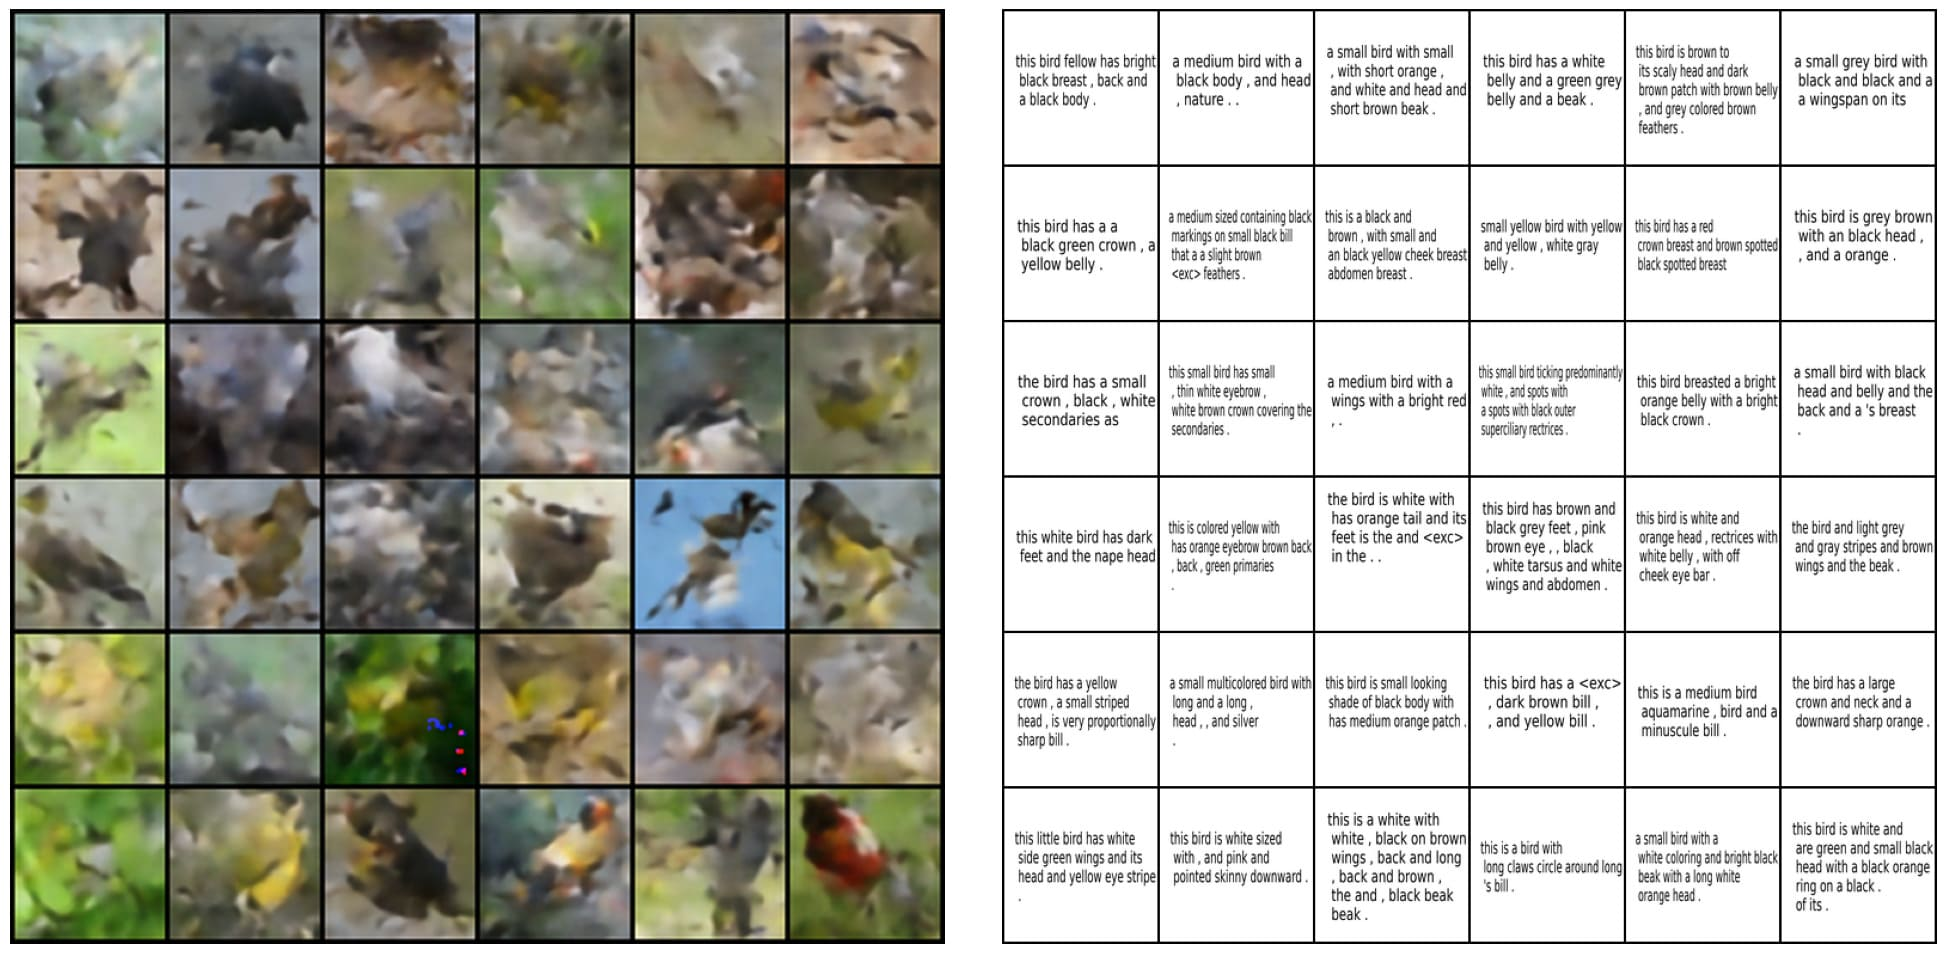
\includegraphics[width=\linewidth]{figures/datasets/cub/mvae_sampling}
        \caption*{\gls{MVAE}}
     \end{subfigure}
     \begin{subfigure}{0.45\textwidth}
         \centering
         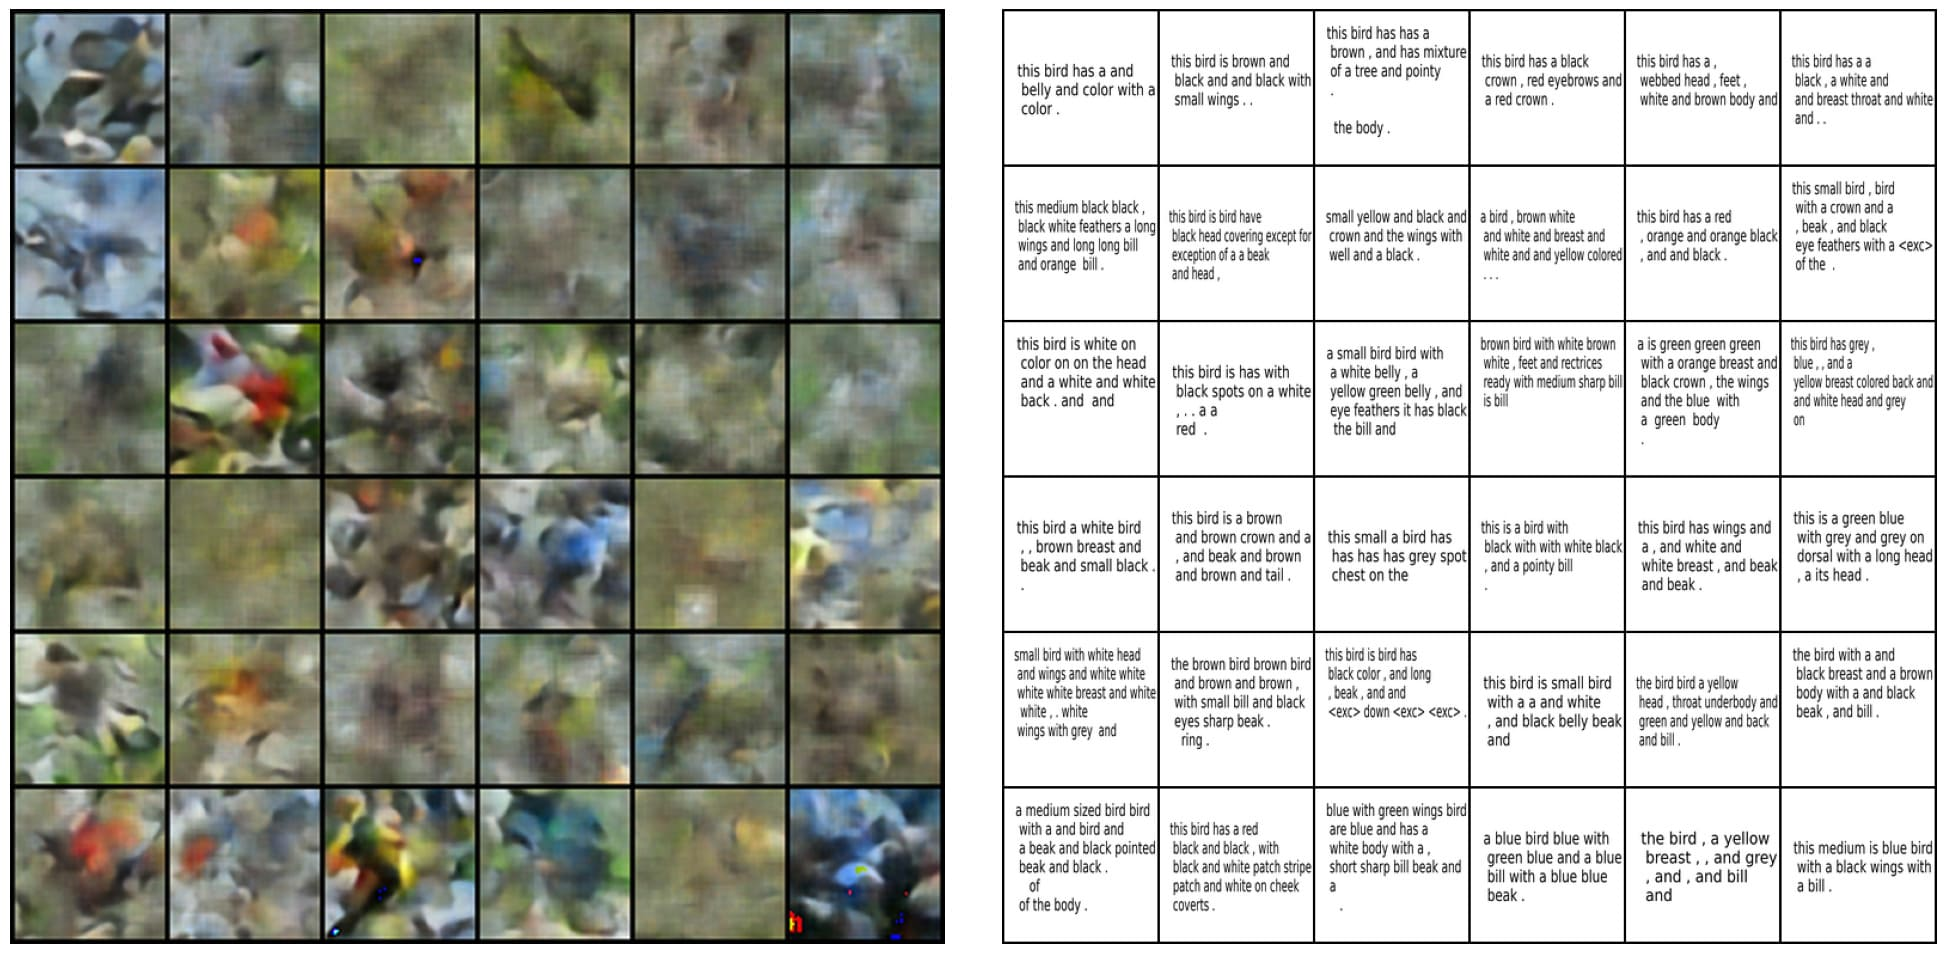
\includegraphics[width=\linewidth]{figures/datasets/cub/mmvae_sampling}
         \caption*{\gls{MMVAE}}
     \end{subfigure}
     
       \begin{subfigure}{0.45\textwidth}
         \centering
         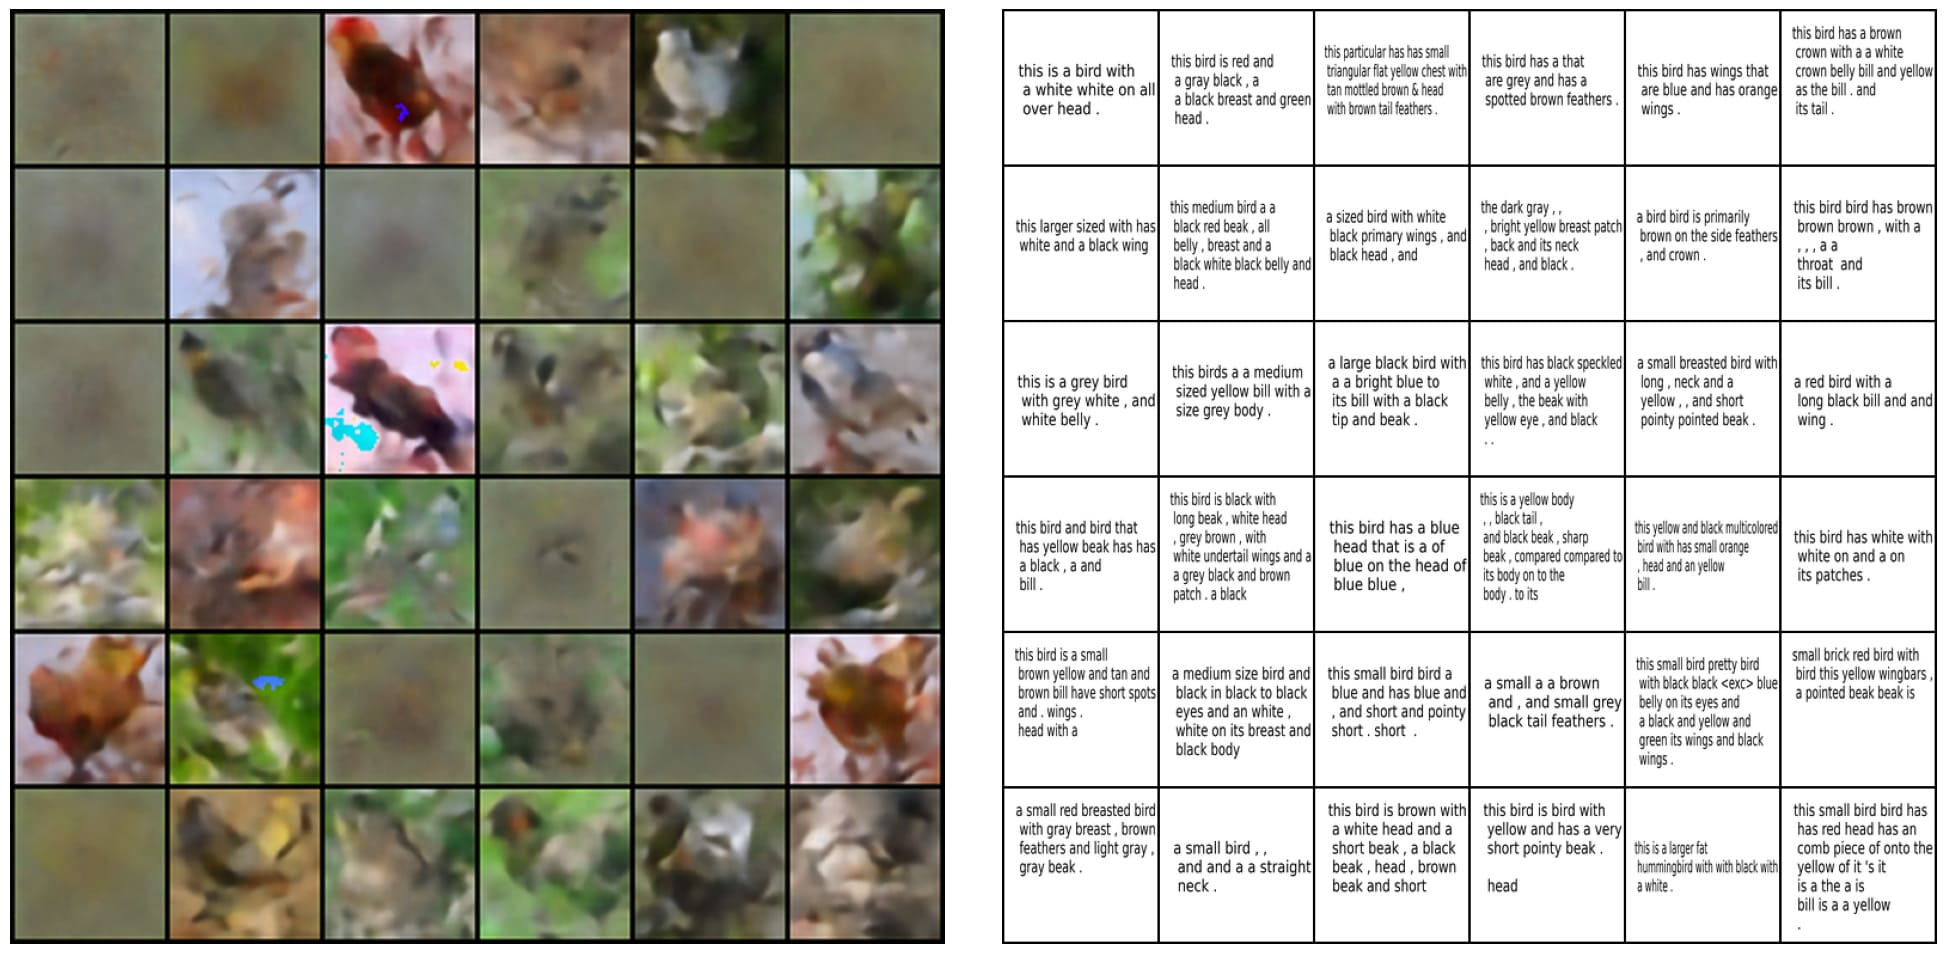
\includegraphics[width=\linewidth]{figures/datasets/cub/mopoe_sampling}
         \caption*{\gls{MOPOE}}
     \end{subfigure}
      \begin{subfigure}{0.45\textwidth}
         \centering
         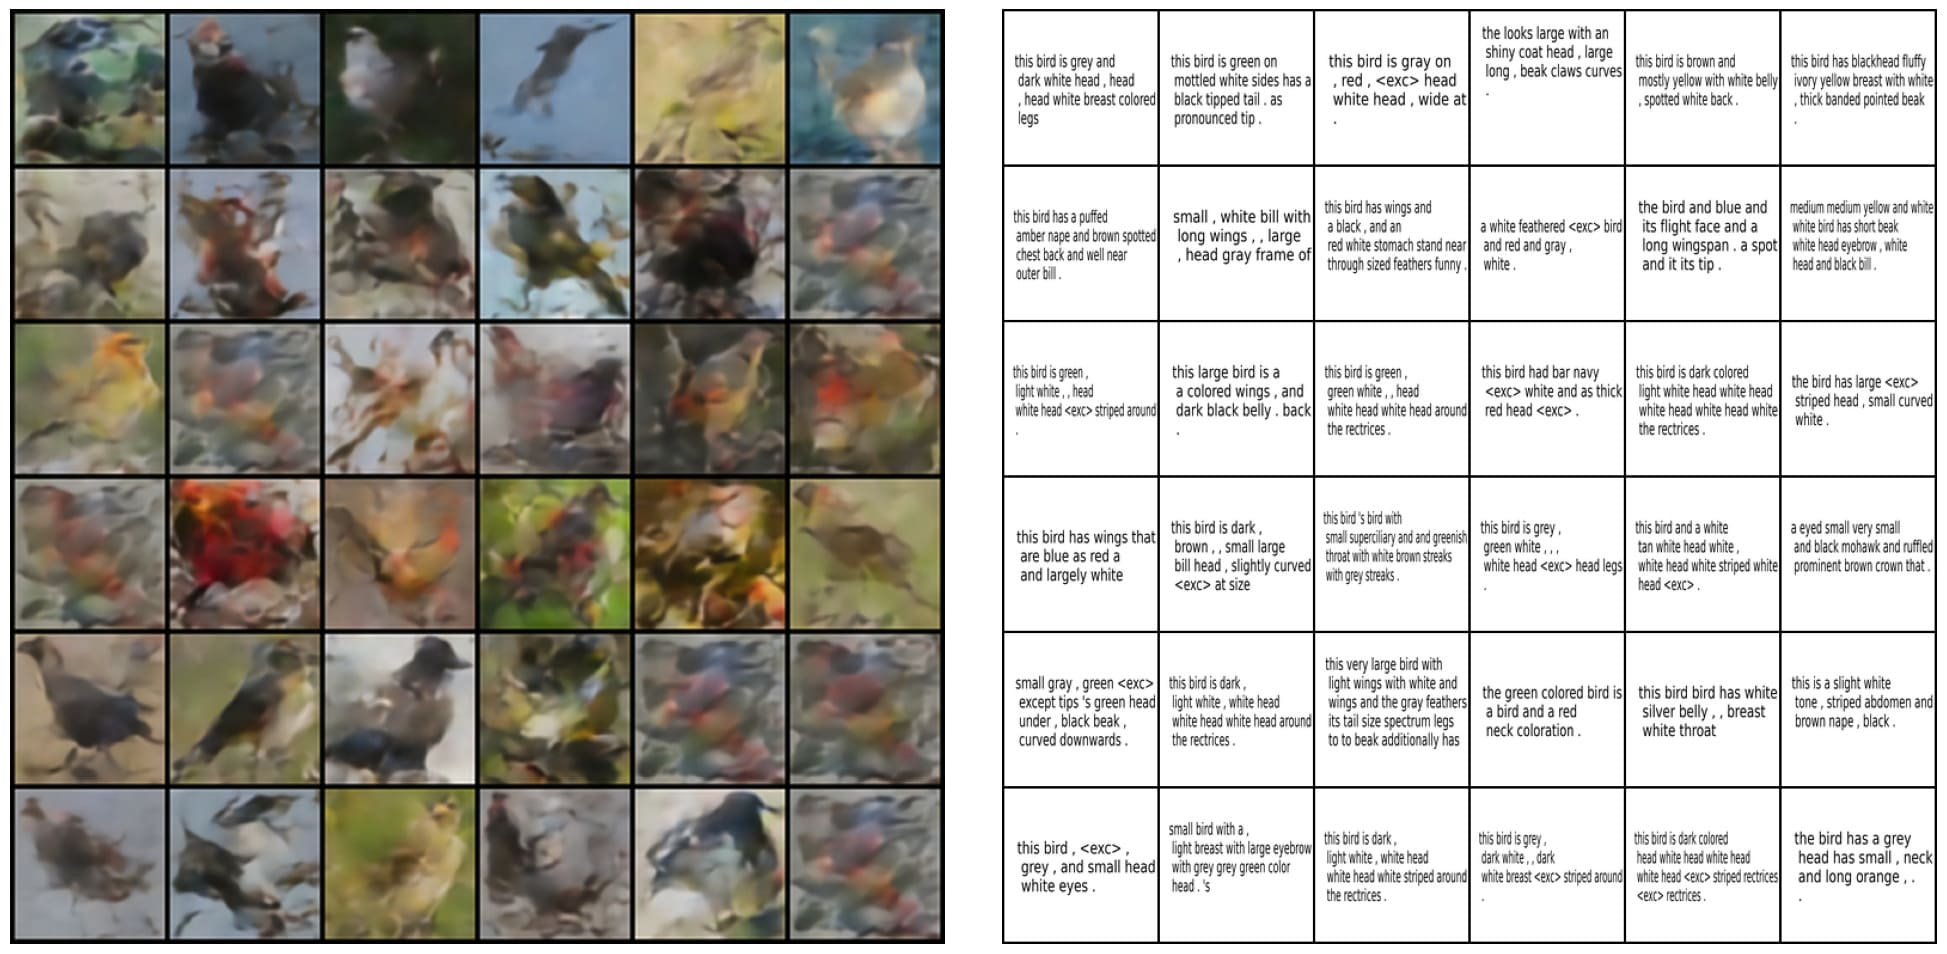
\includegraphics[width=\linewidth]{figures/datasets/cub/nexus_sampling}
         \caption*{\gls{NEXUS}}
     \end{subfigure}
     
     \begin{subfigure}{0.45\textwidth}
         \centering
         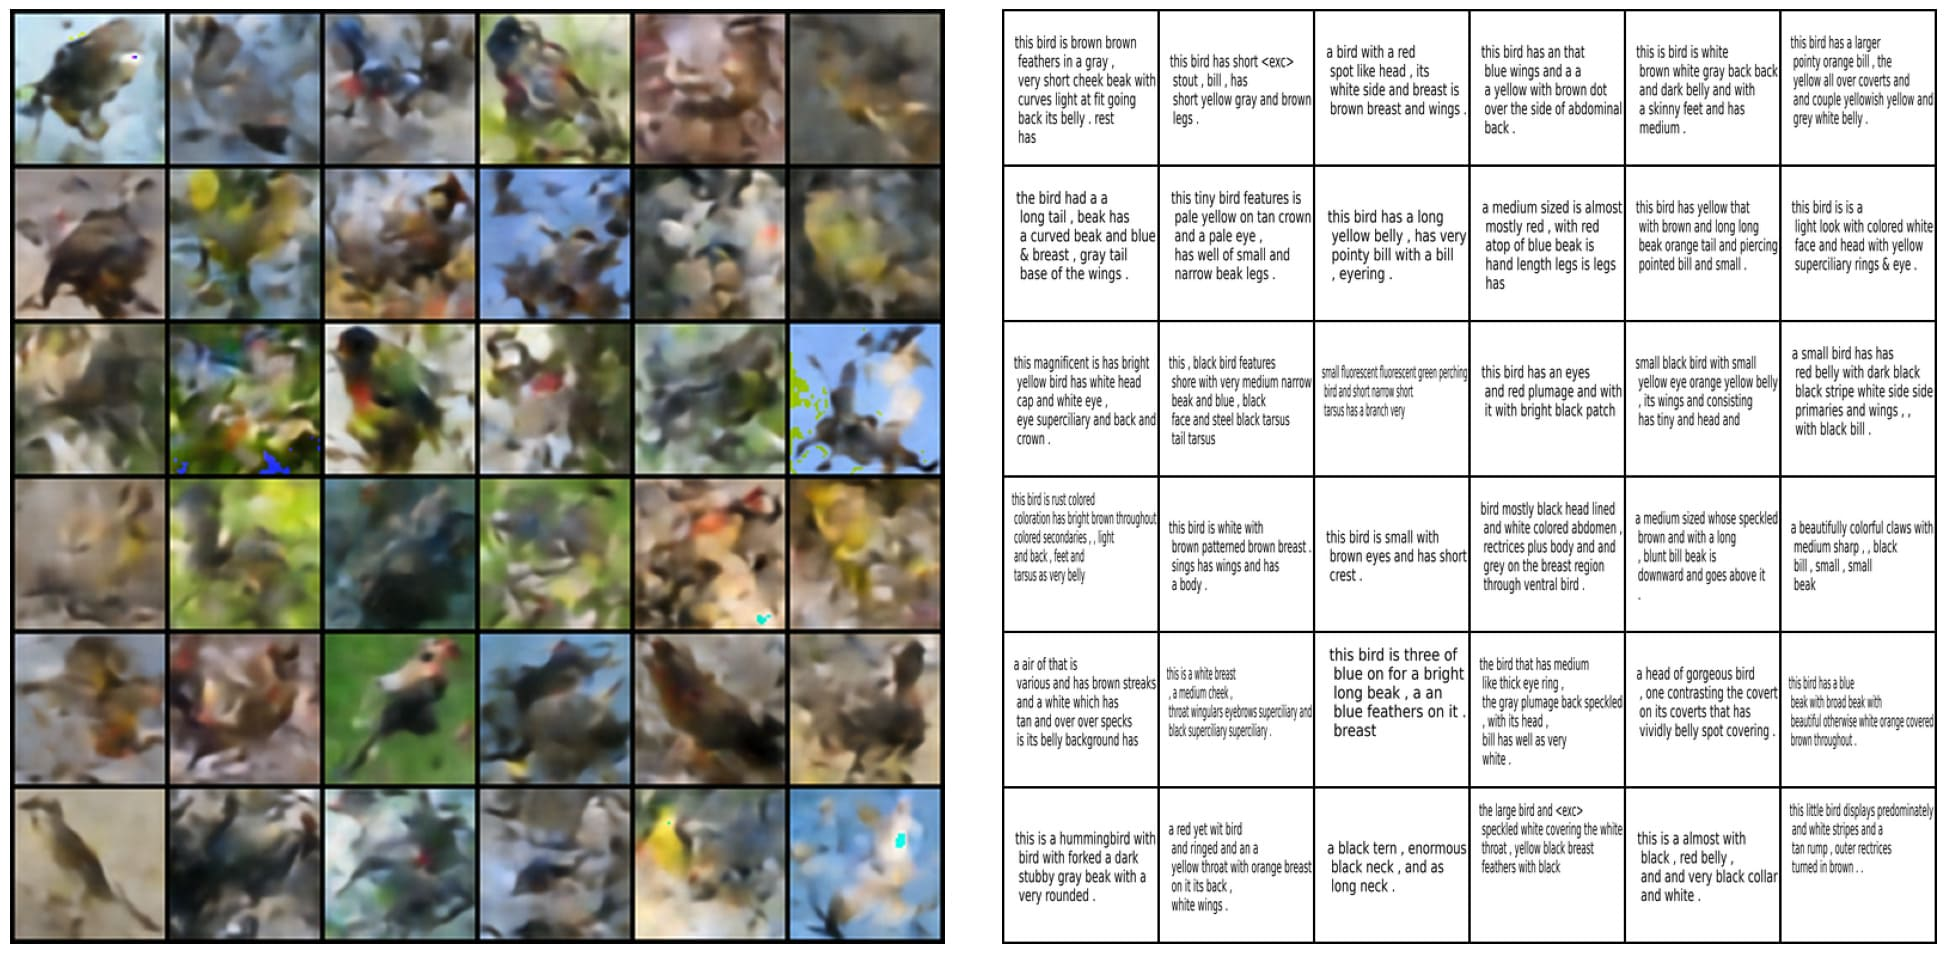
\includegraphics[width=\linewidth]{figures/datasets/cub/mvtcae_sampling}
         \caption*{\gls{MVTCAE}}
     \end{subfigure}
 \begin{subfigure}{0.45\textwidth}
         \centering
        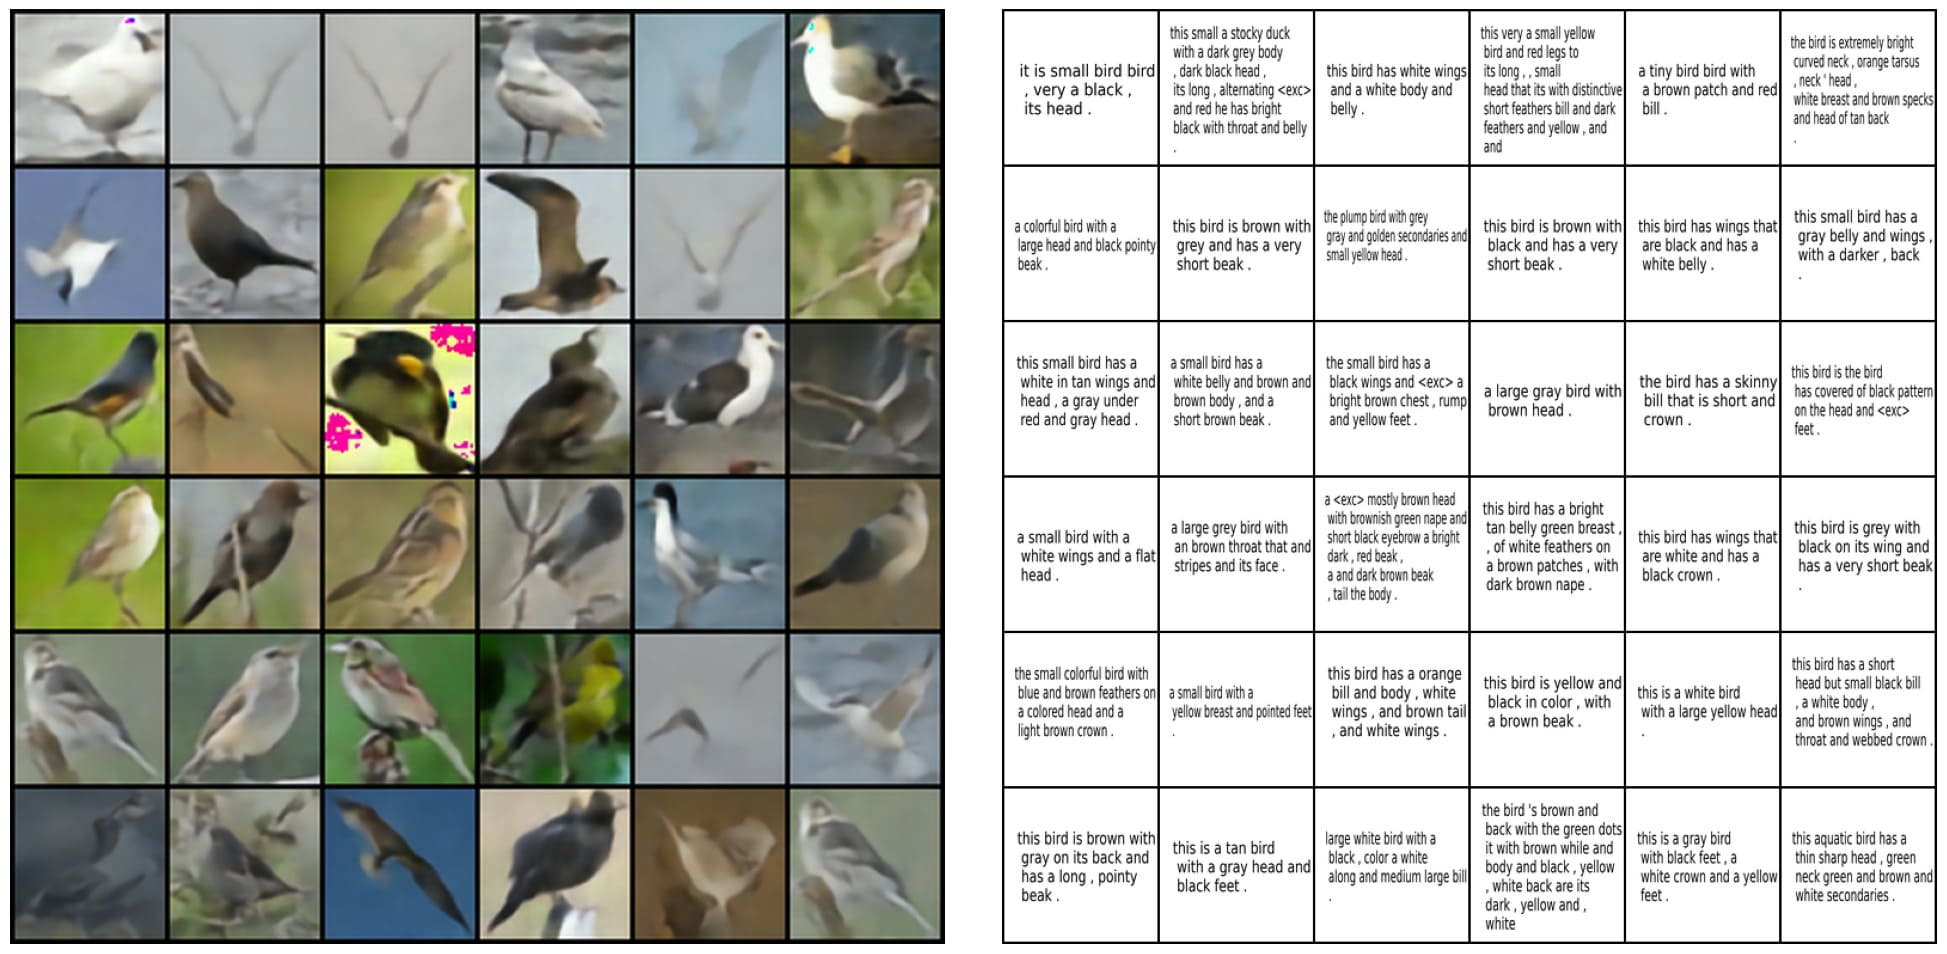
\includegraphics[page=1,width=\linewidth]{figures/datasets/cub/MLD_inpaint_sampling}
         \caption*{\gls{MLD Inpaint}  }
\end{subfigure}

 \begin{subfigure}{0.45\textwidth}
         \centering
         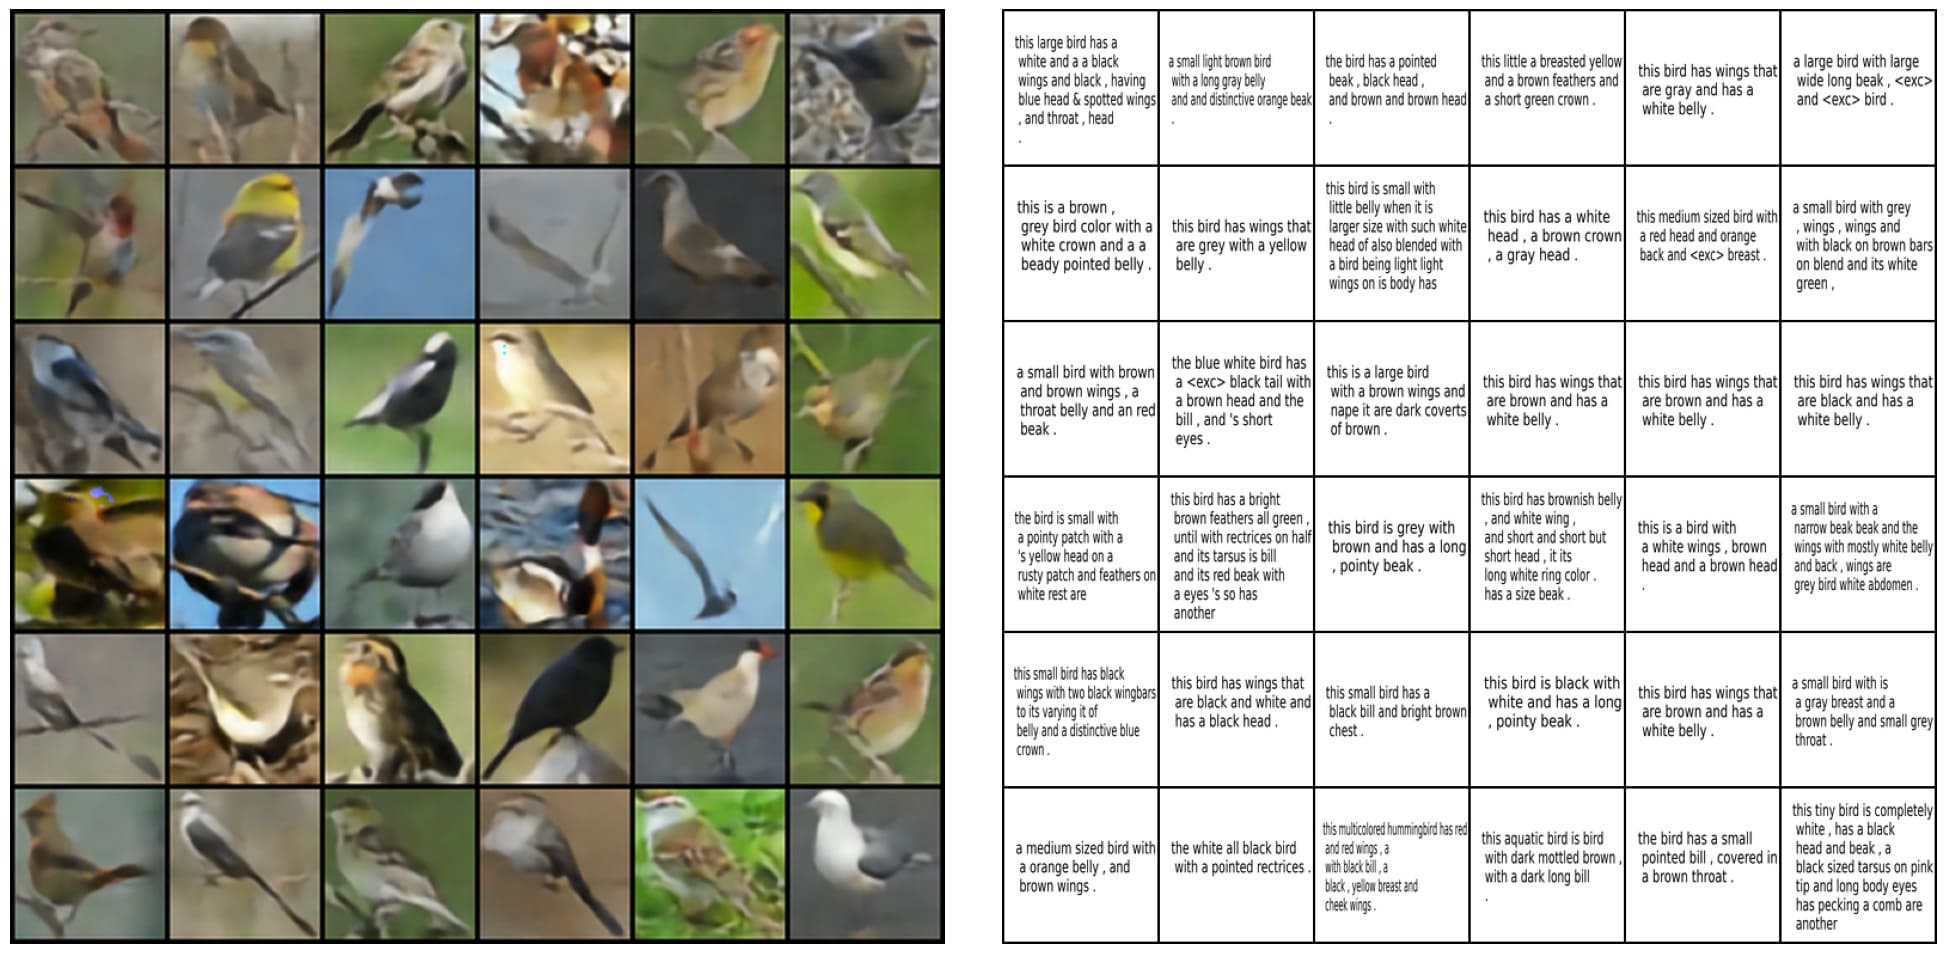
\includegraphics[page=1,width=\linewidth]{figures/datasets/cub/MLD_uni_sampling}
         \caption*{\gls{MLD Uni}  }
\end{subfigure}
\begin{subfigure}{0.45\textwidth}
    \centering
    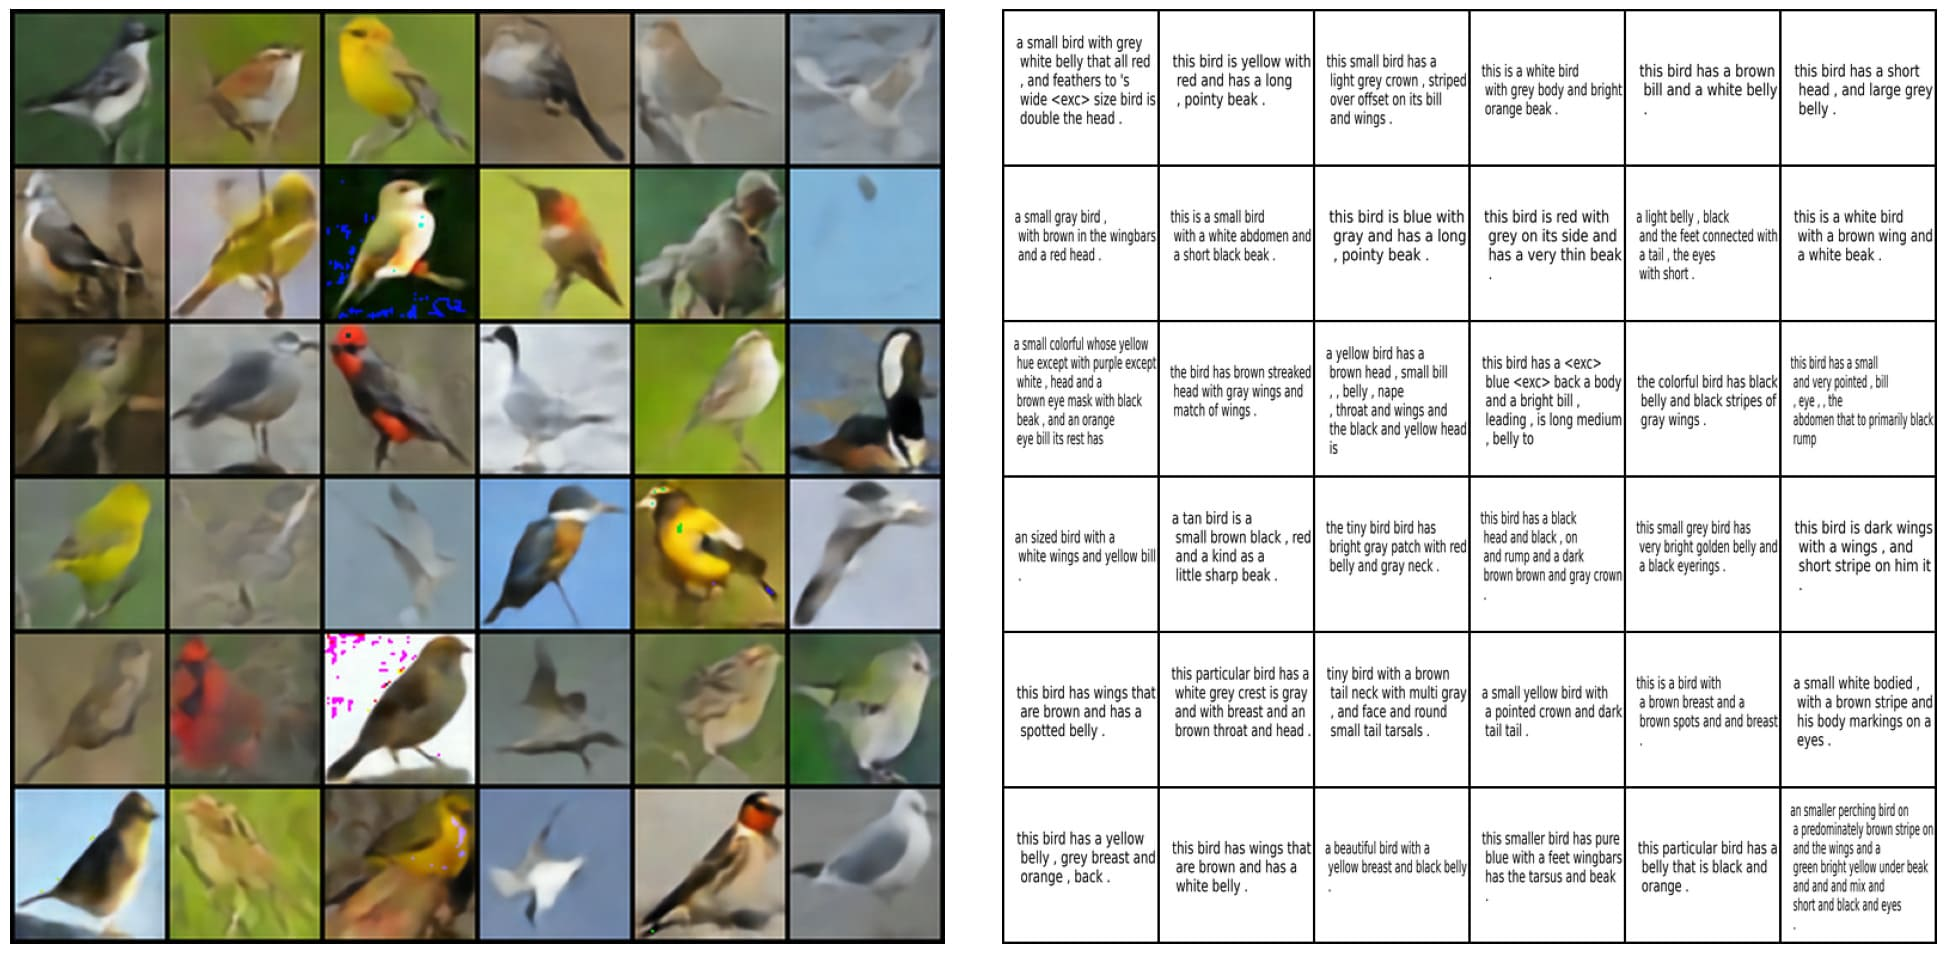
\includegraphics[page=1,width=\linewidth]{figures/datasets/cub/MLD_sampling}
    \caption*{\gls{MLD} (ours) }
\end{subfigure}
\caption{Qualitative results for joint generation on \textbf{\cub}.}
\label{cap_joint_detailed}
        
\end{figure}


    

% \begin{figure}[h]
%      \centering
%      \begin{subfigure}{0.3\textwidth}
%          \centering
%          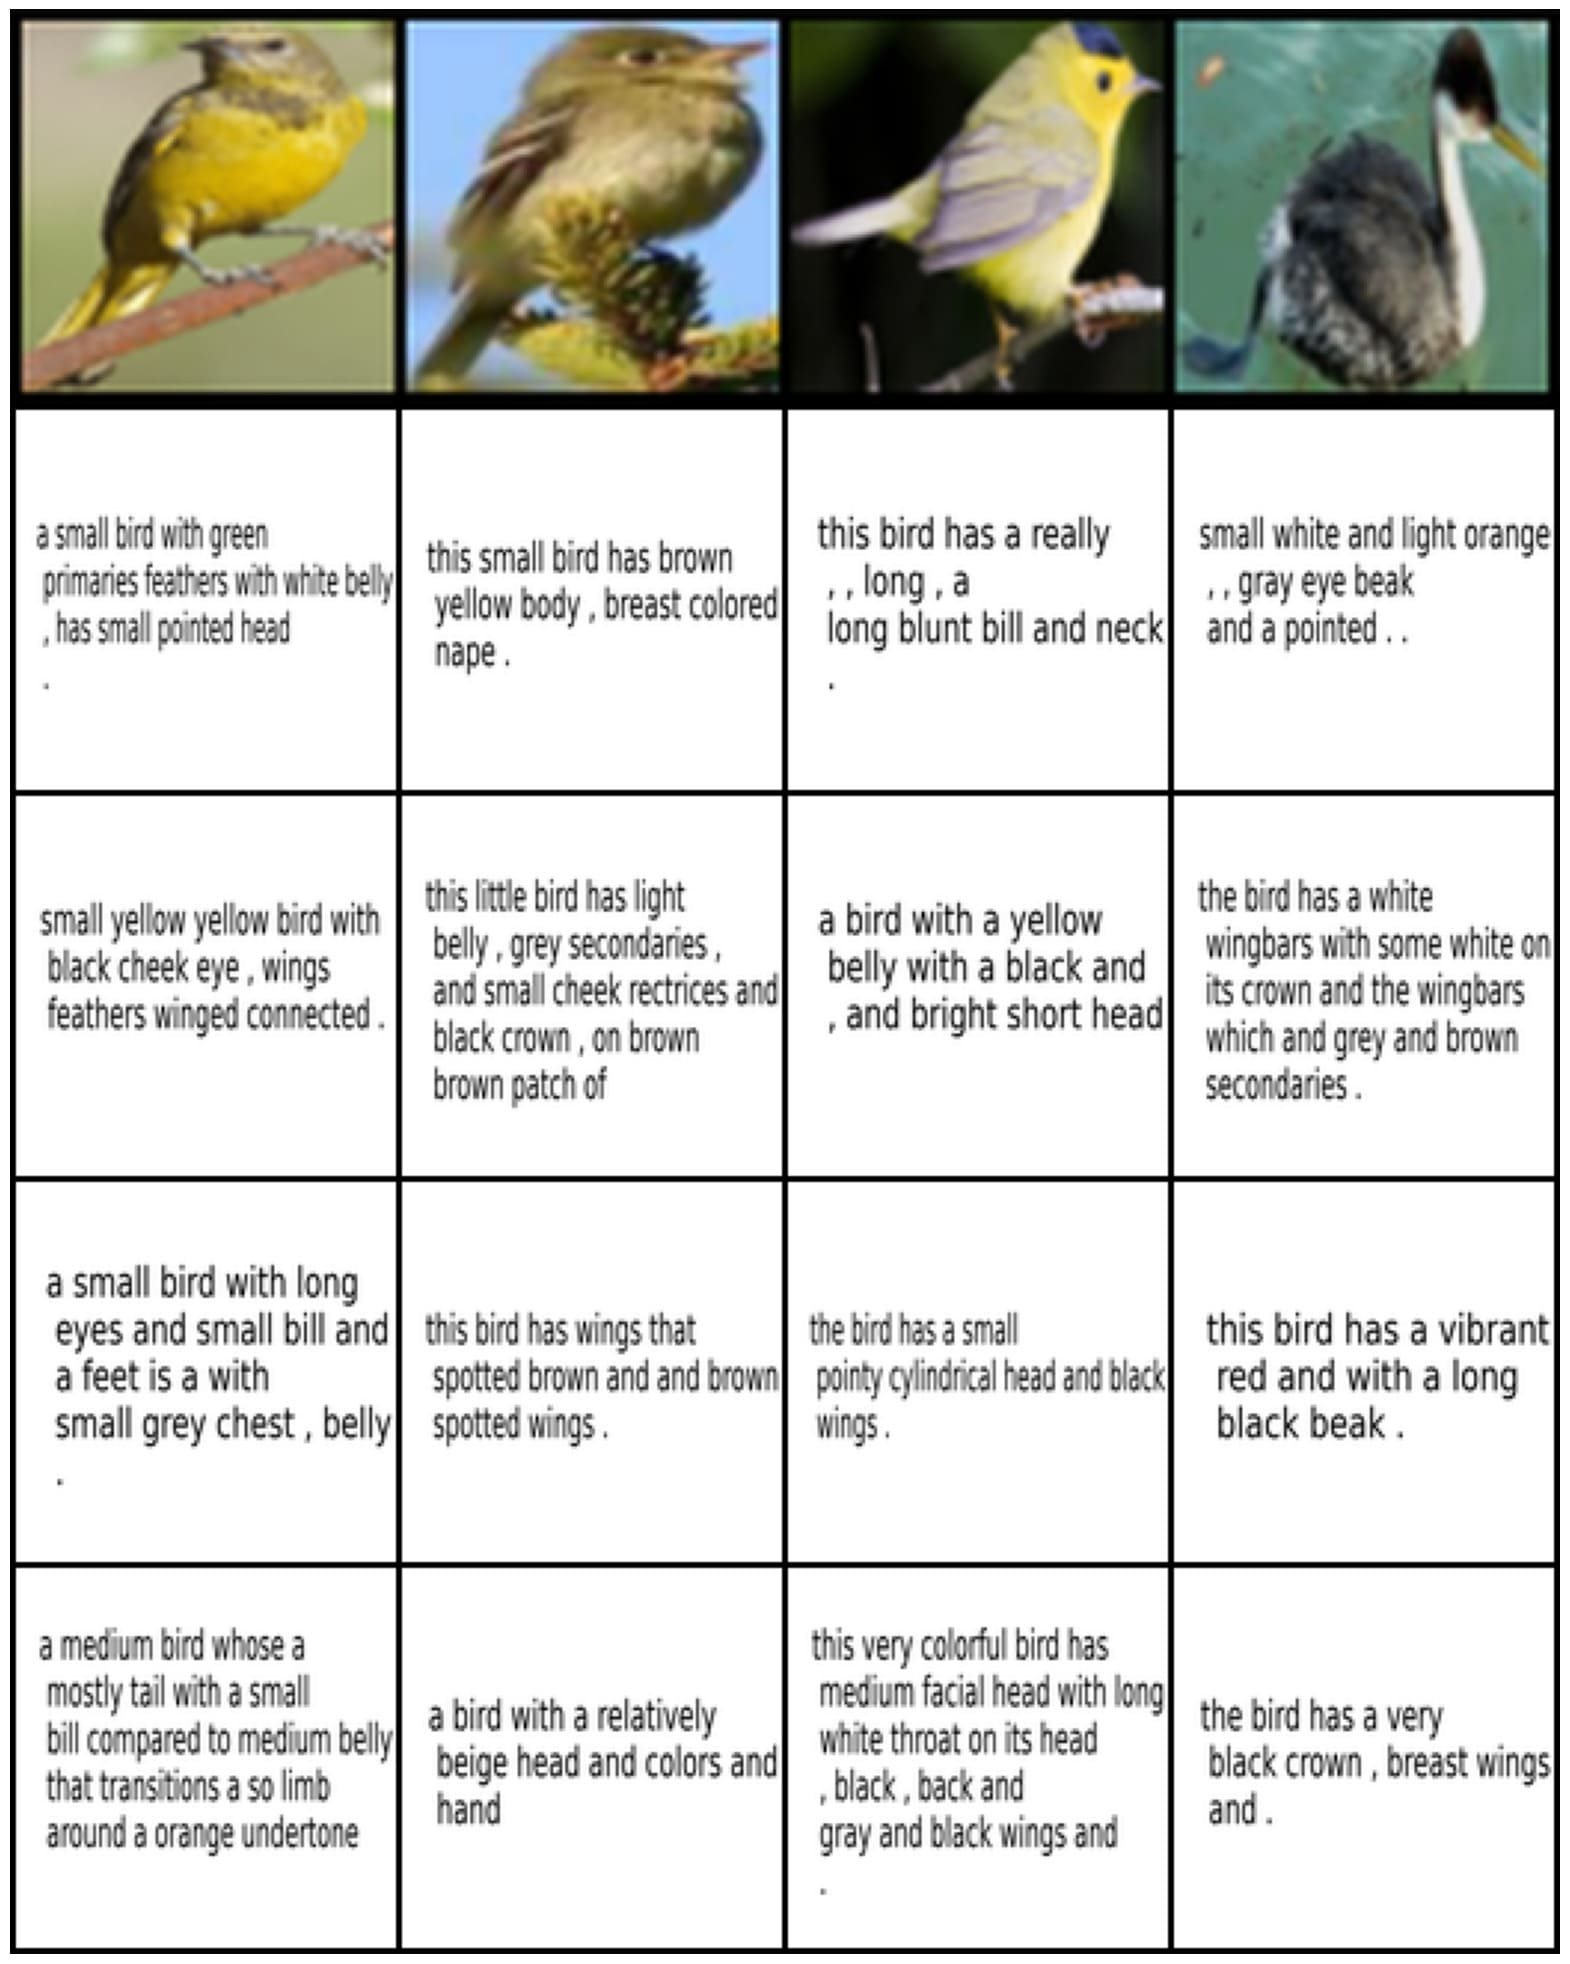
\includegraphics[width=\linewidth]{figures/datasets/cub/mvae_cond_image_text}
%         \caption*{\gls{MVAE}}
%      \end{subfigure}
%      \begin{subfigure}{0.3\textwidth}
%          \centering
%          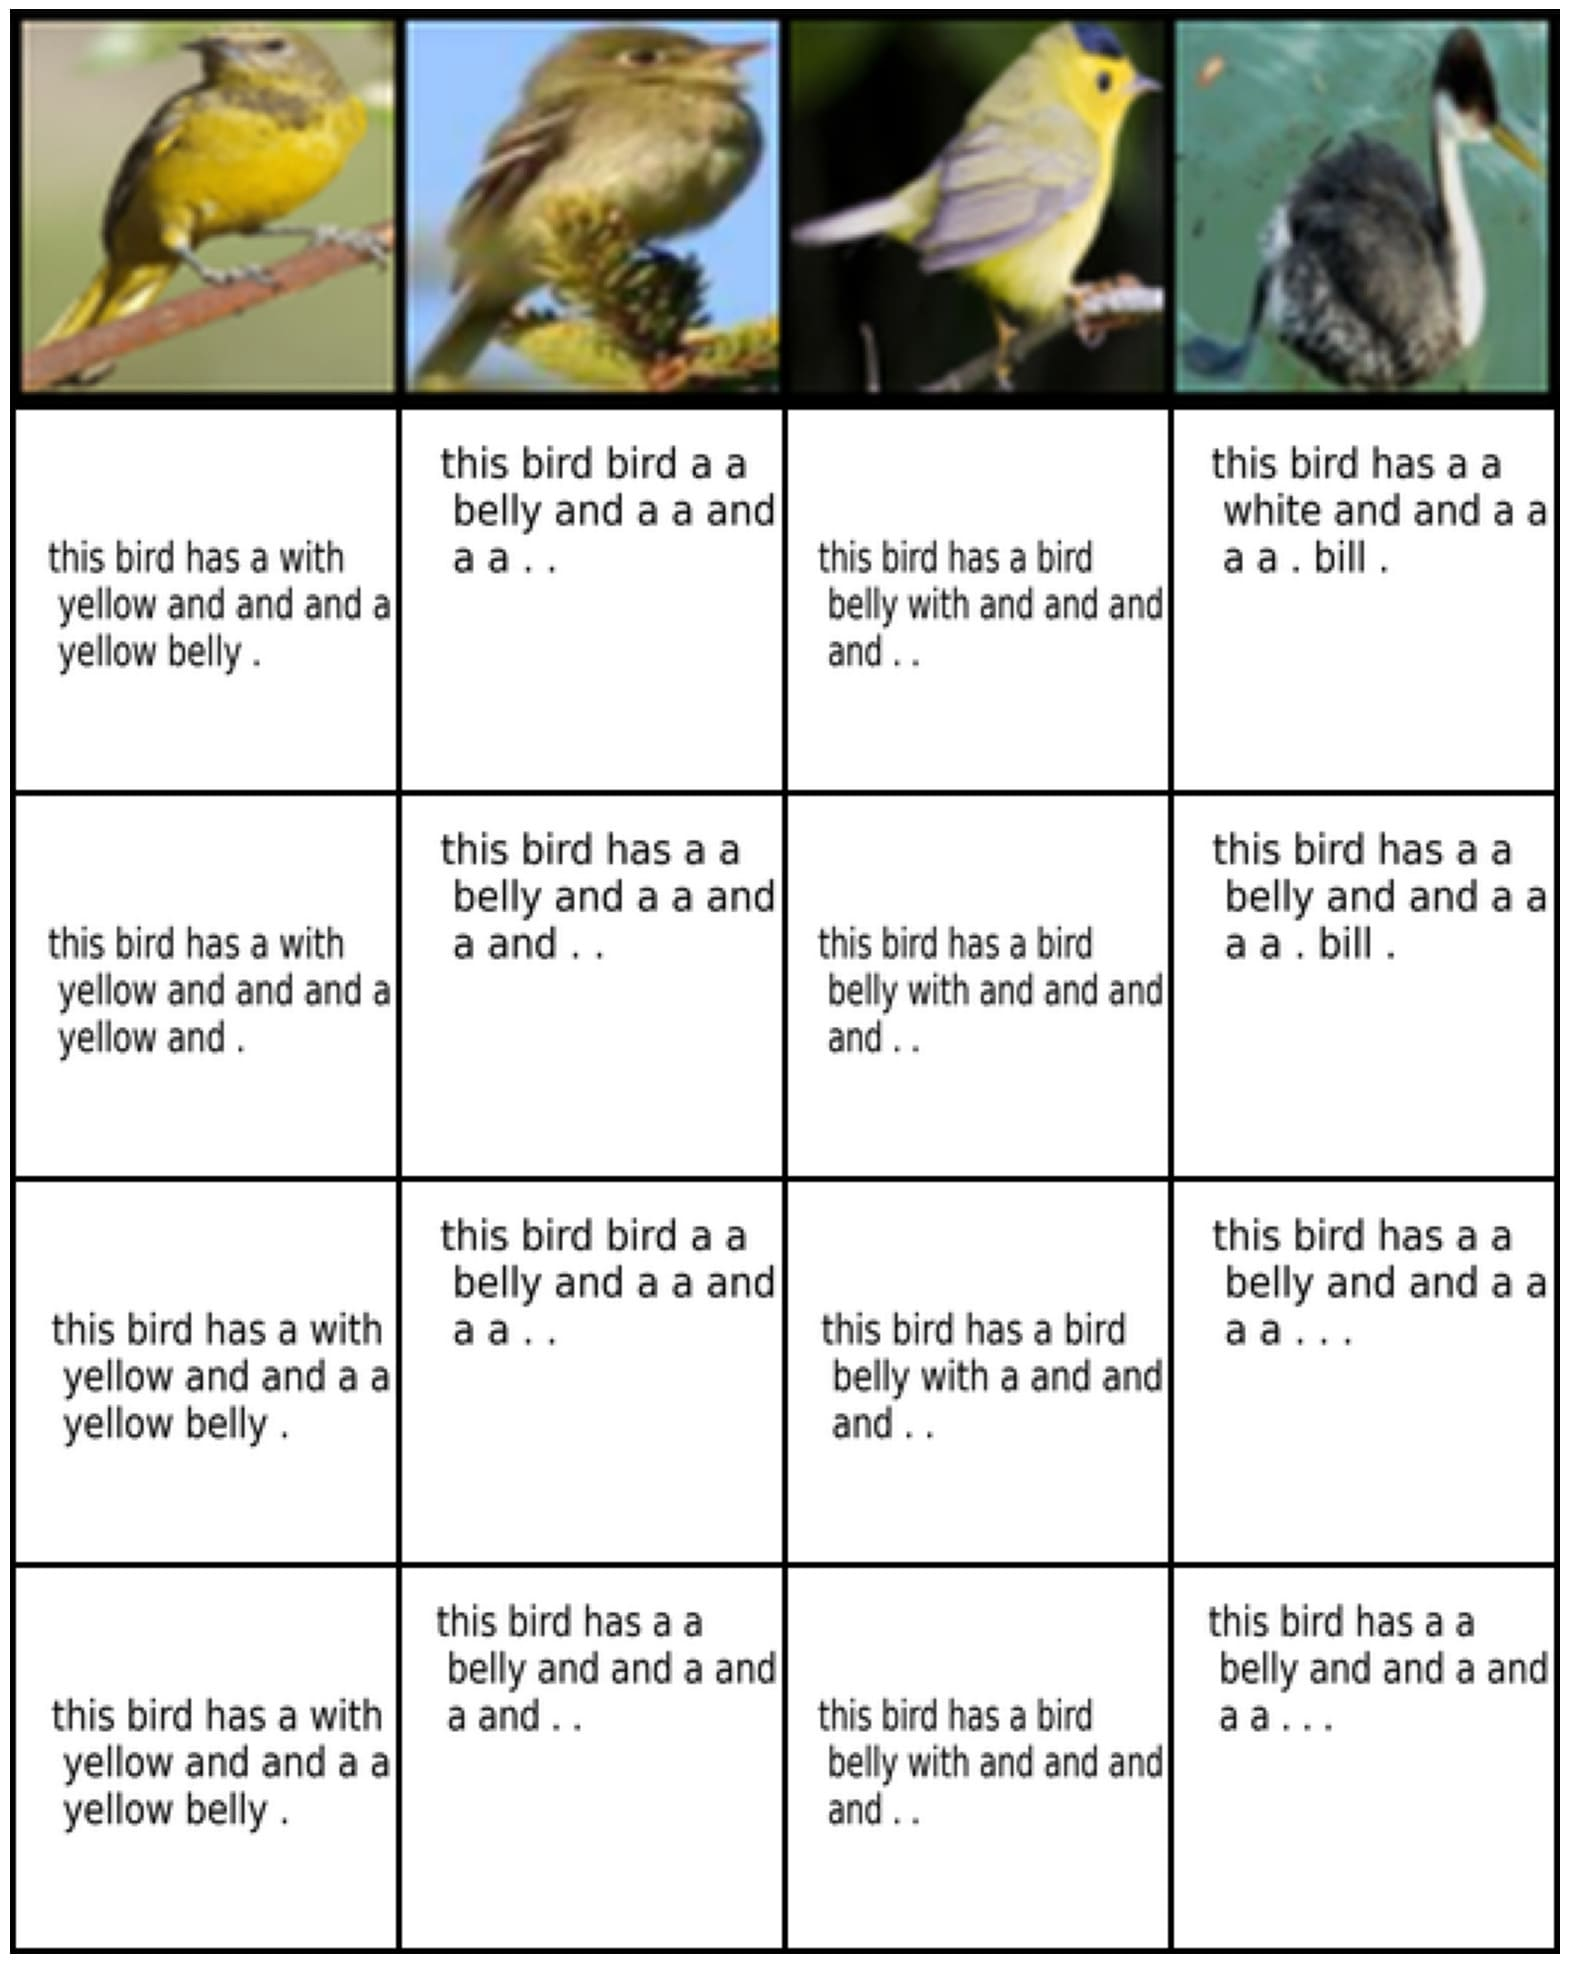
\includegraphics[width=\linewidth]{figures/datasets/cub/mmvae_cond_image_text}
%          \caption*{\gls{MMVAE}}
%      \end{subfigure}
%        \begin{subfigure}{0.3\textwidth}
%          \centering
%          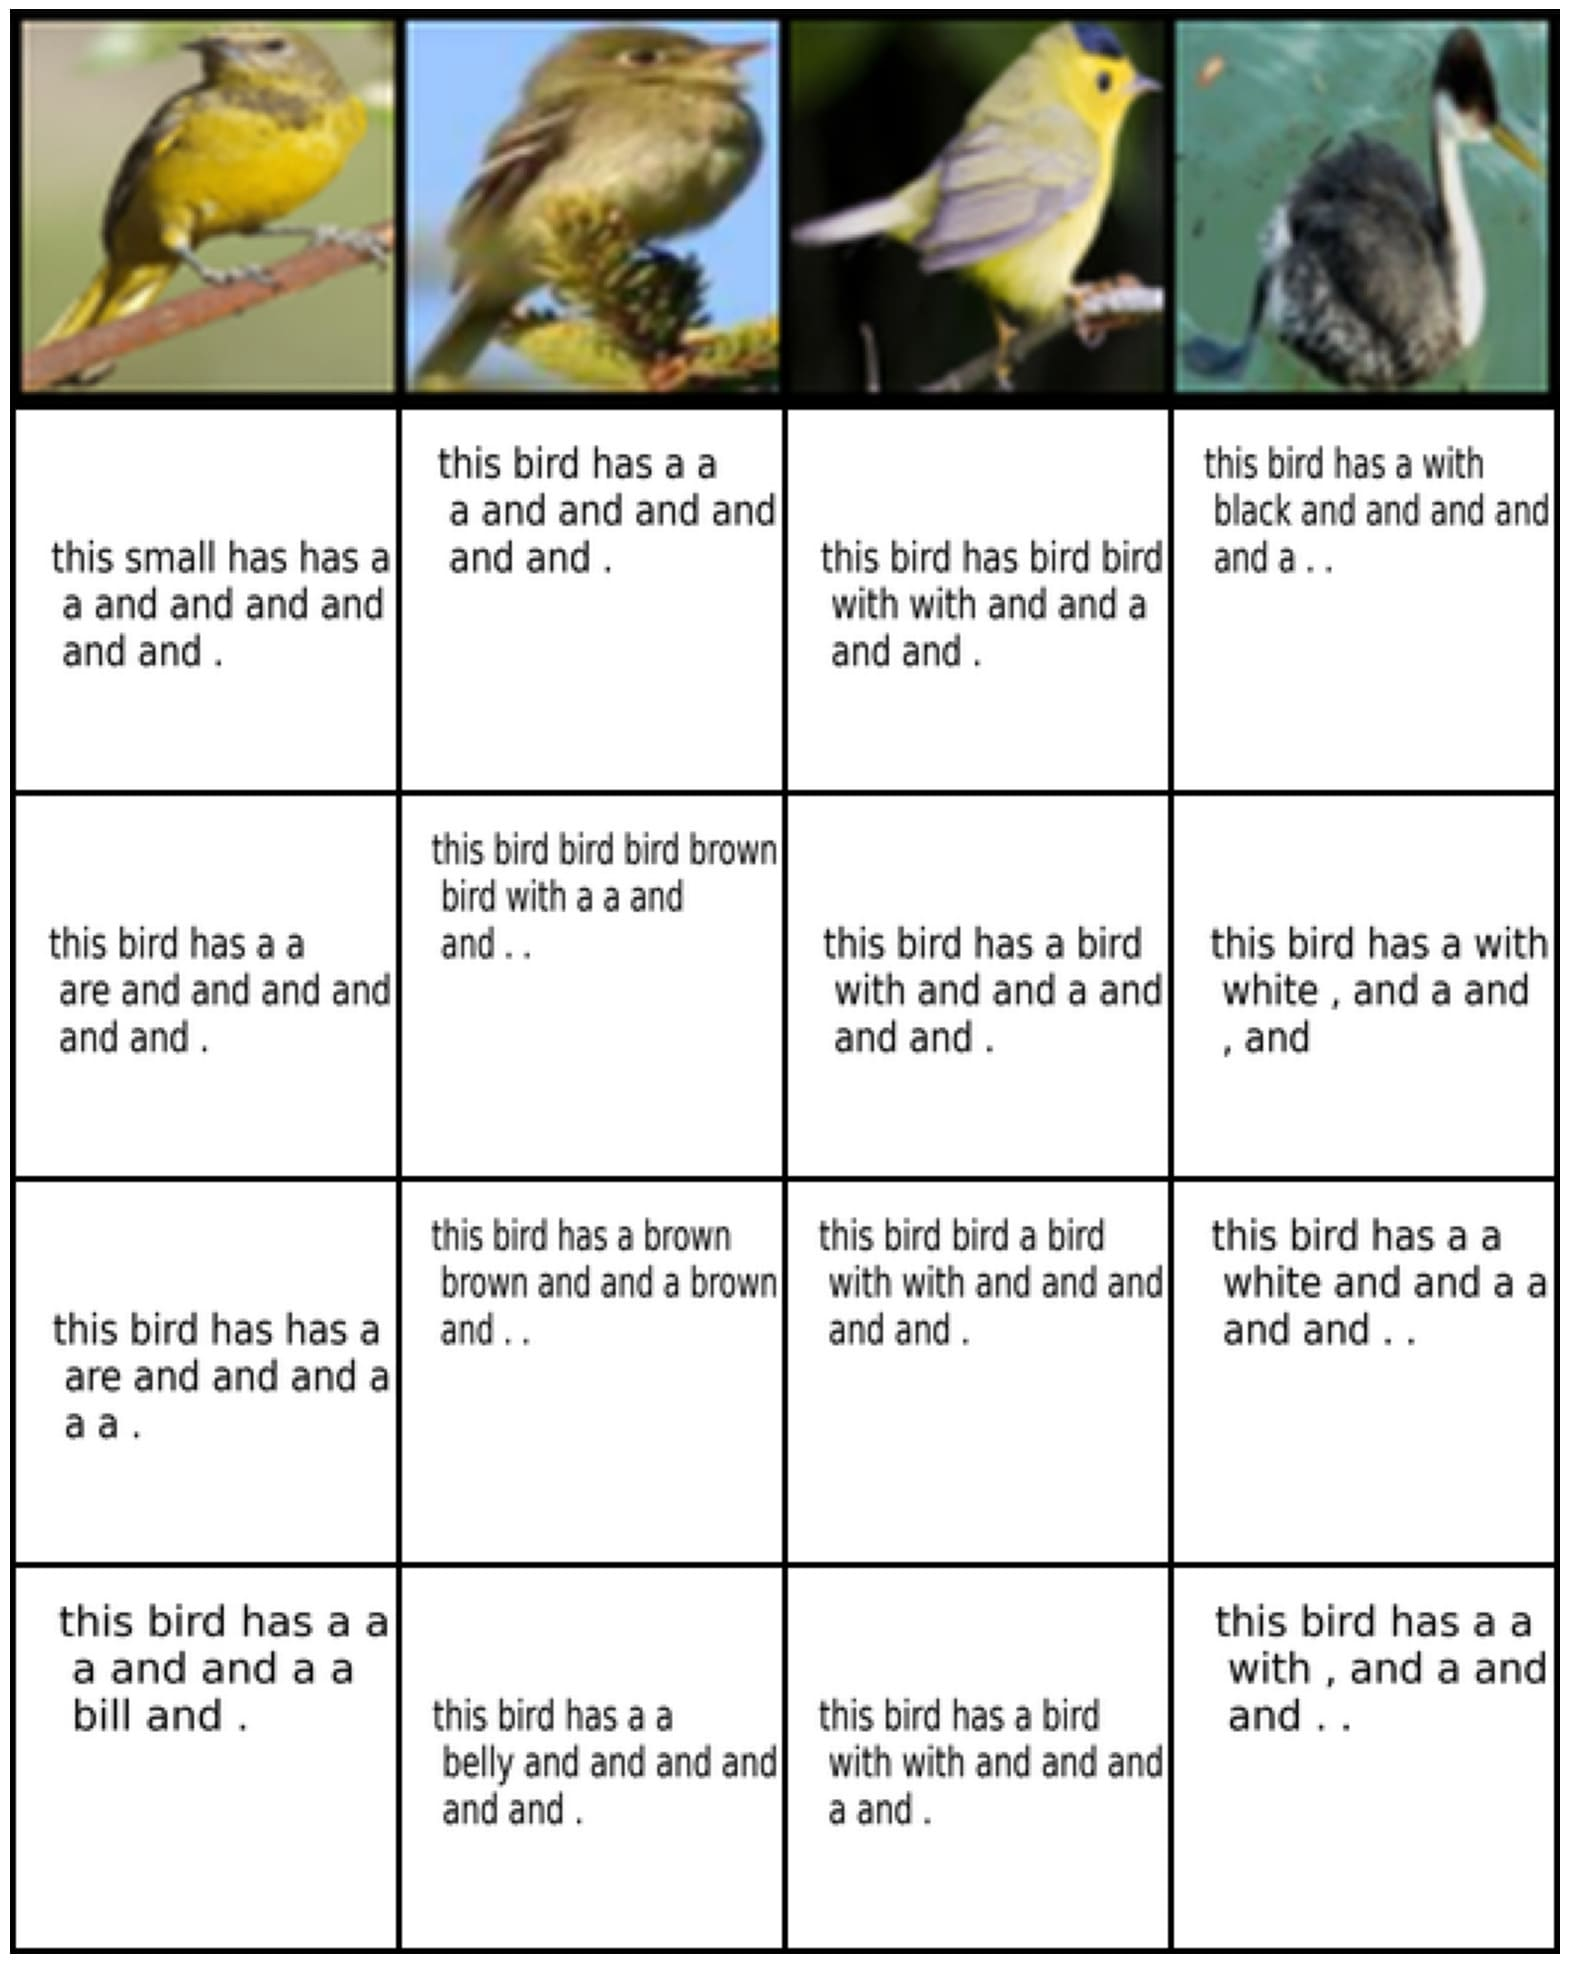
\includegraphics[width=\linewidth]{figures/datasets/cub/mopoe_cond_image_text}
%          \caption*{\gls{MOPOE}}
%      \end{subfigure}
     
%       \begin{subfigure}{0.3\textwidth}
%          \centering
%          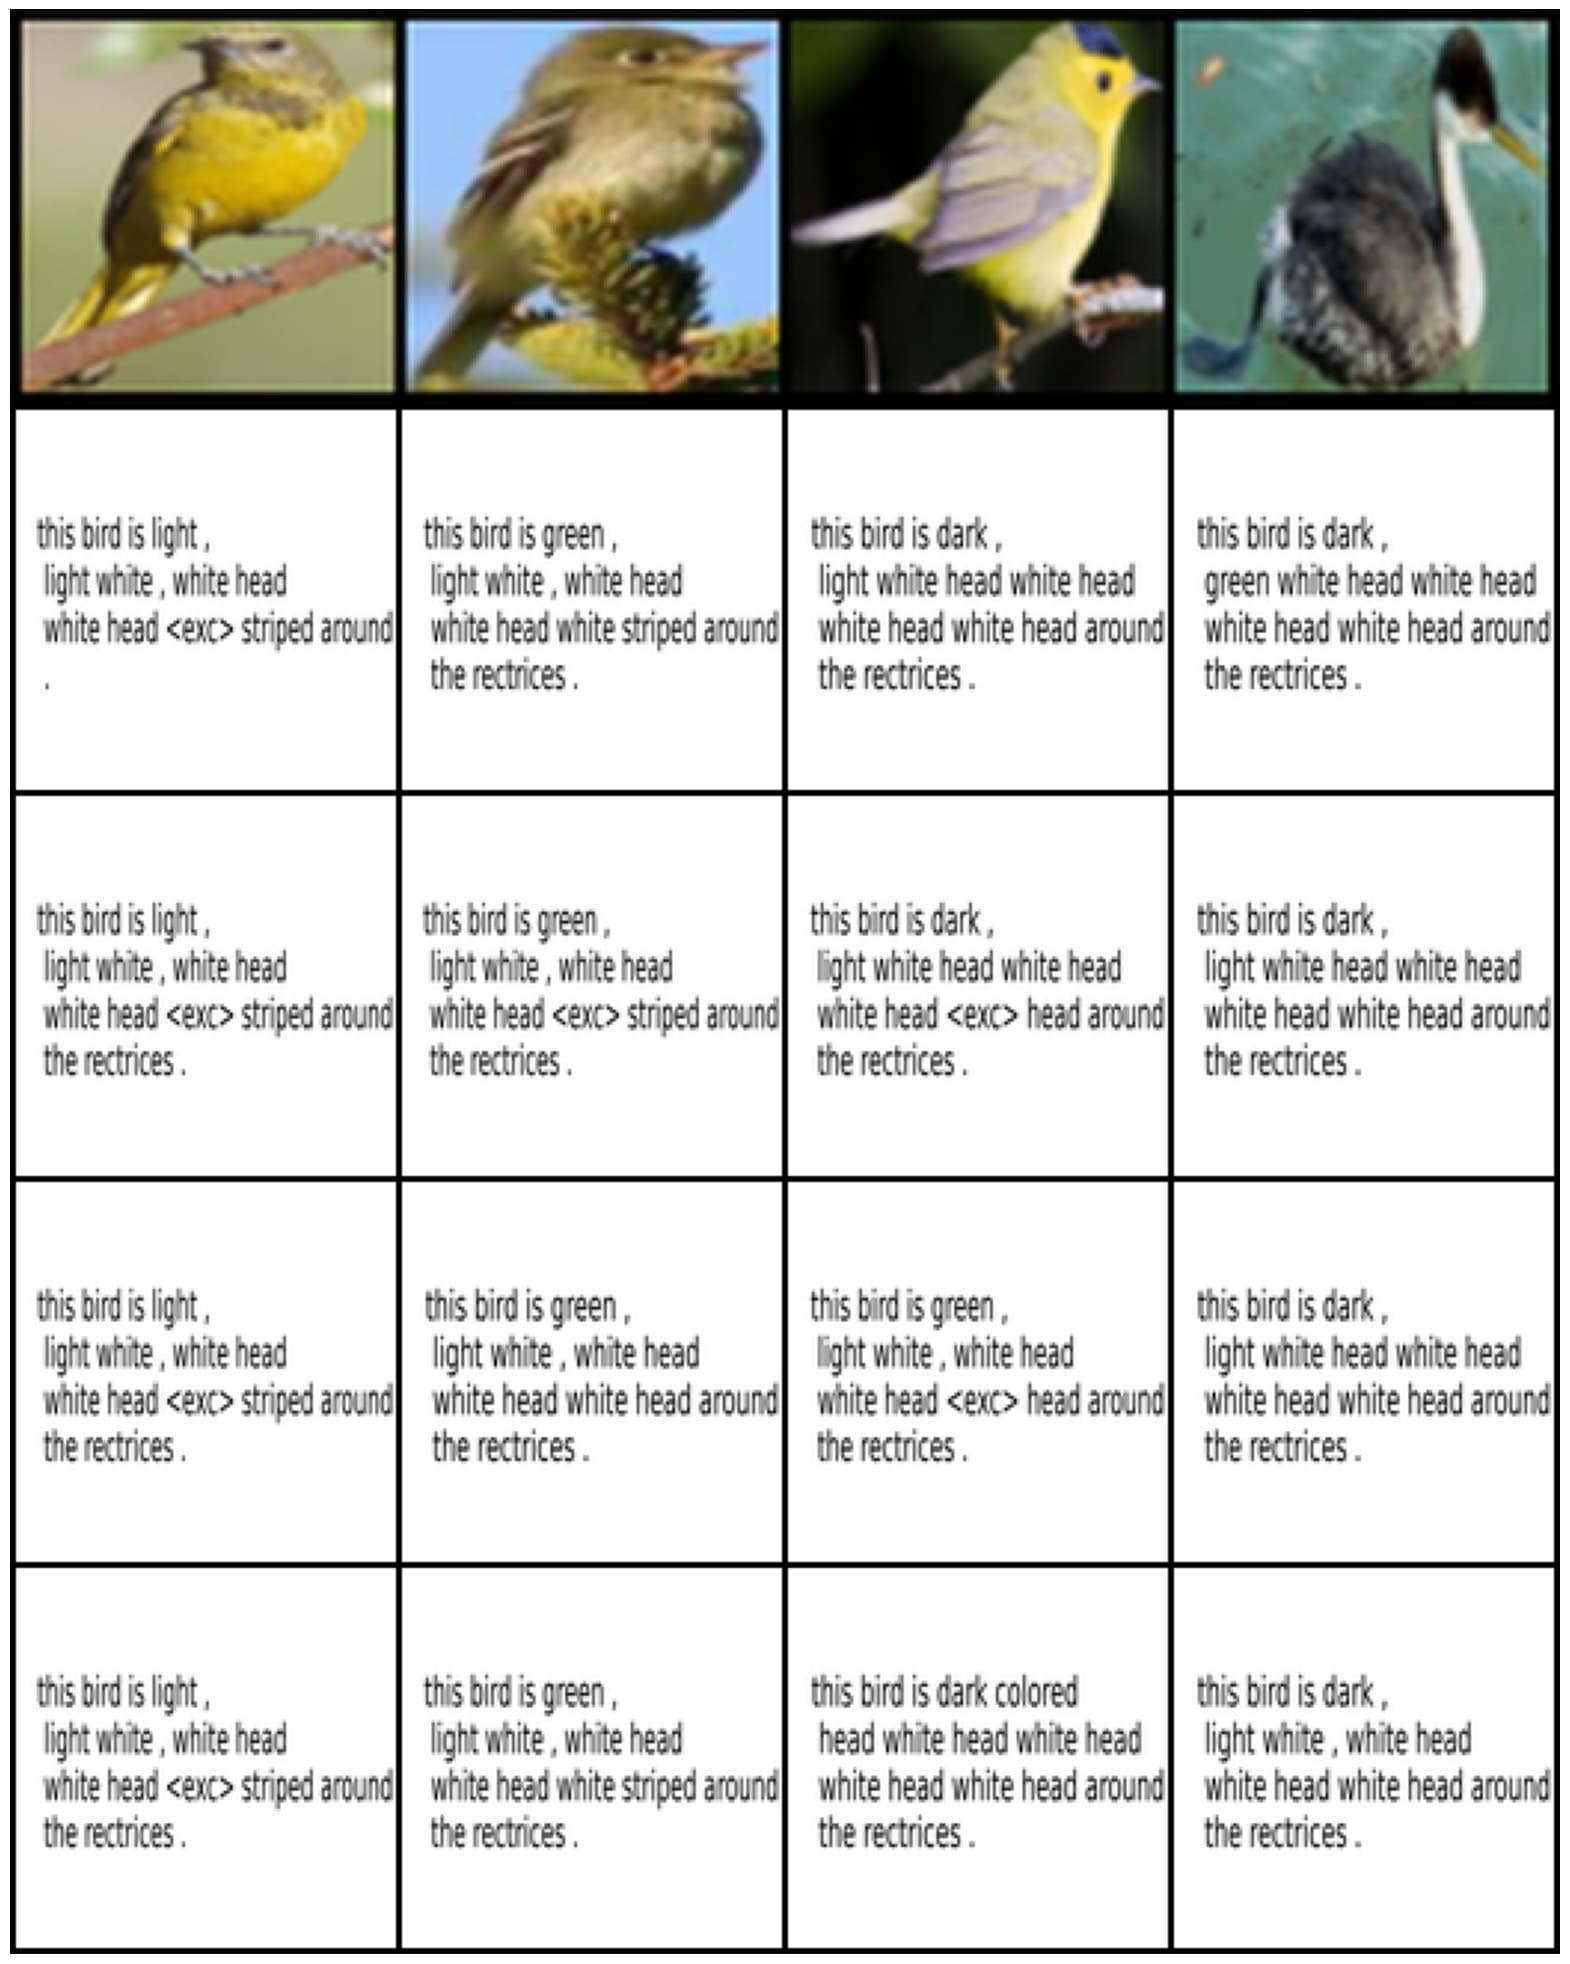
\includegraphics[width=\linewidth]{figures/datasets/cub/nexus_cond_image_text}
%          \caption*{\gls{NEXUS}}
%      \end{subfigure}
%      \begin{subfigure}{0.3\textwidth}
%          \centering
%          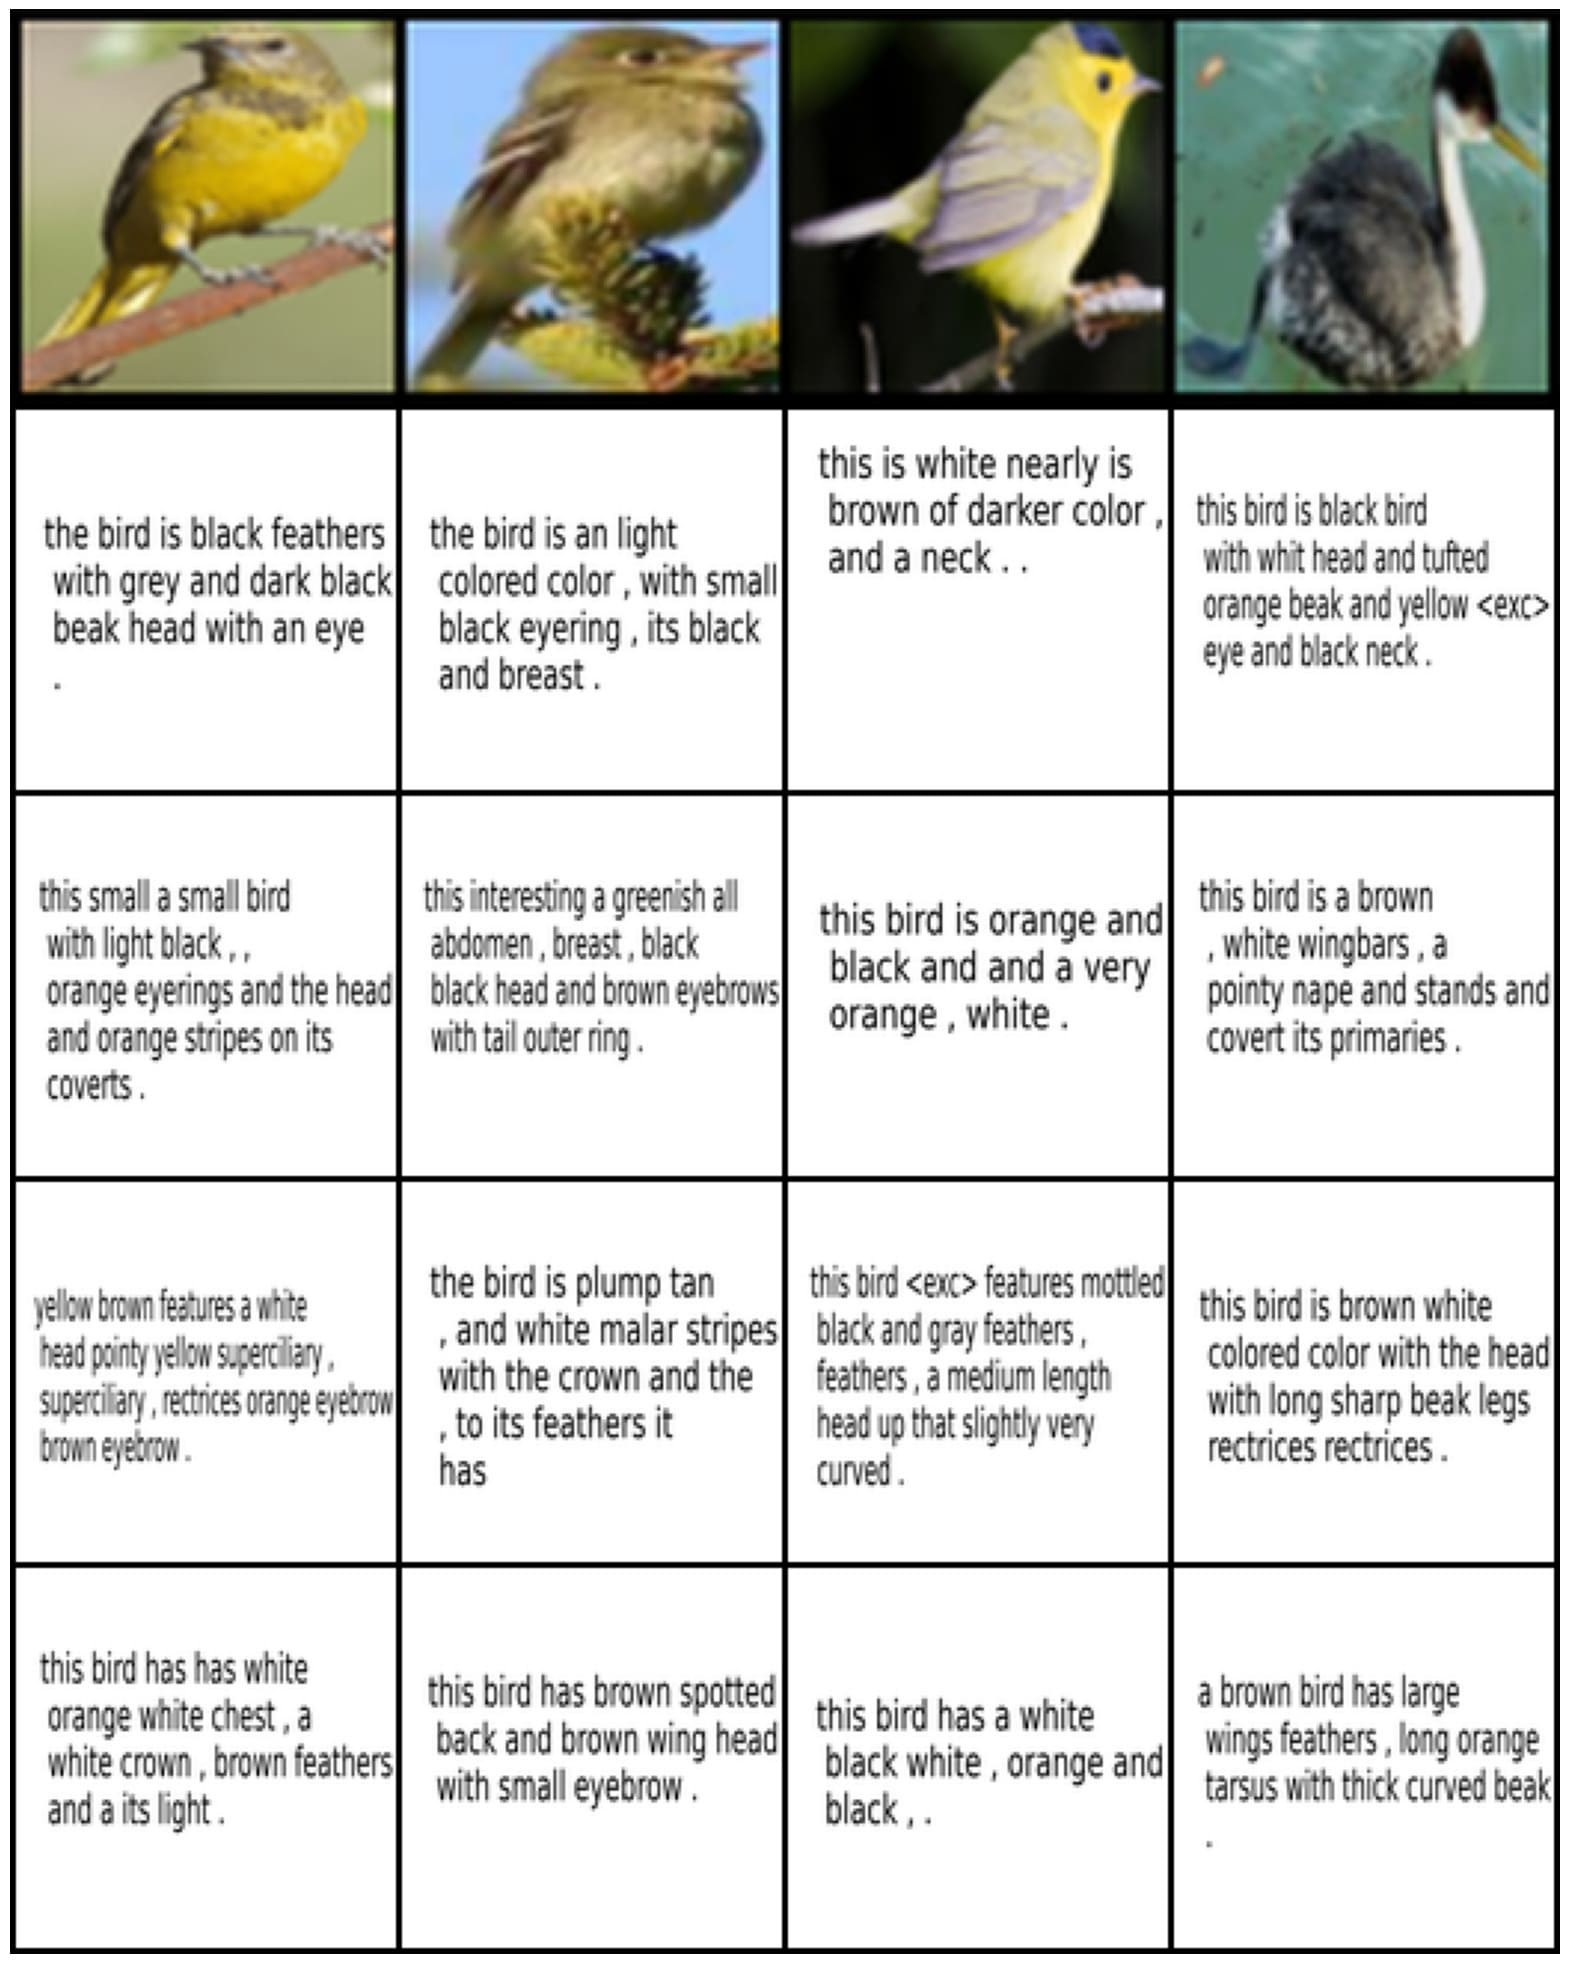
\includegraphics[width=\linewidth]{figures/datasets/cub/mvtcae_cond_image_text}
%          \caption*{\gls{MVTCAE}}
%      \end{subfigure}
%  \begin{subfigure}{0.3\textwidth}
%          \centering
%         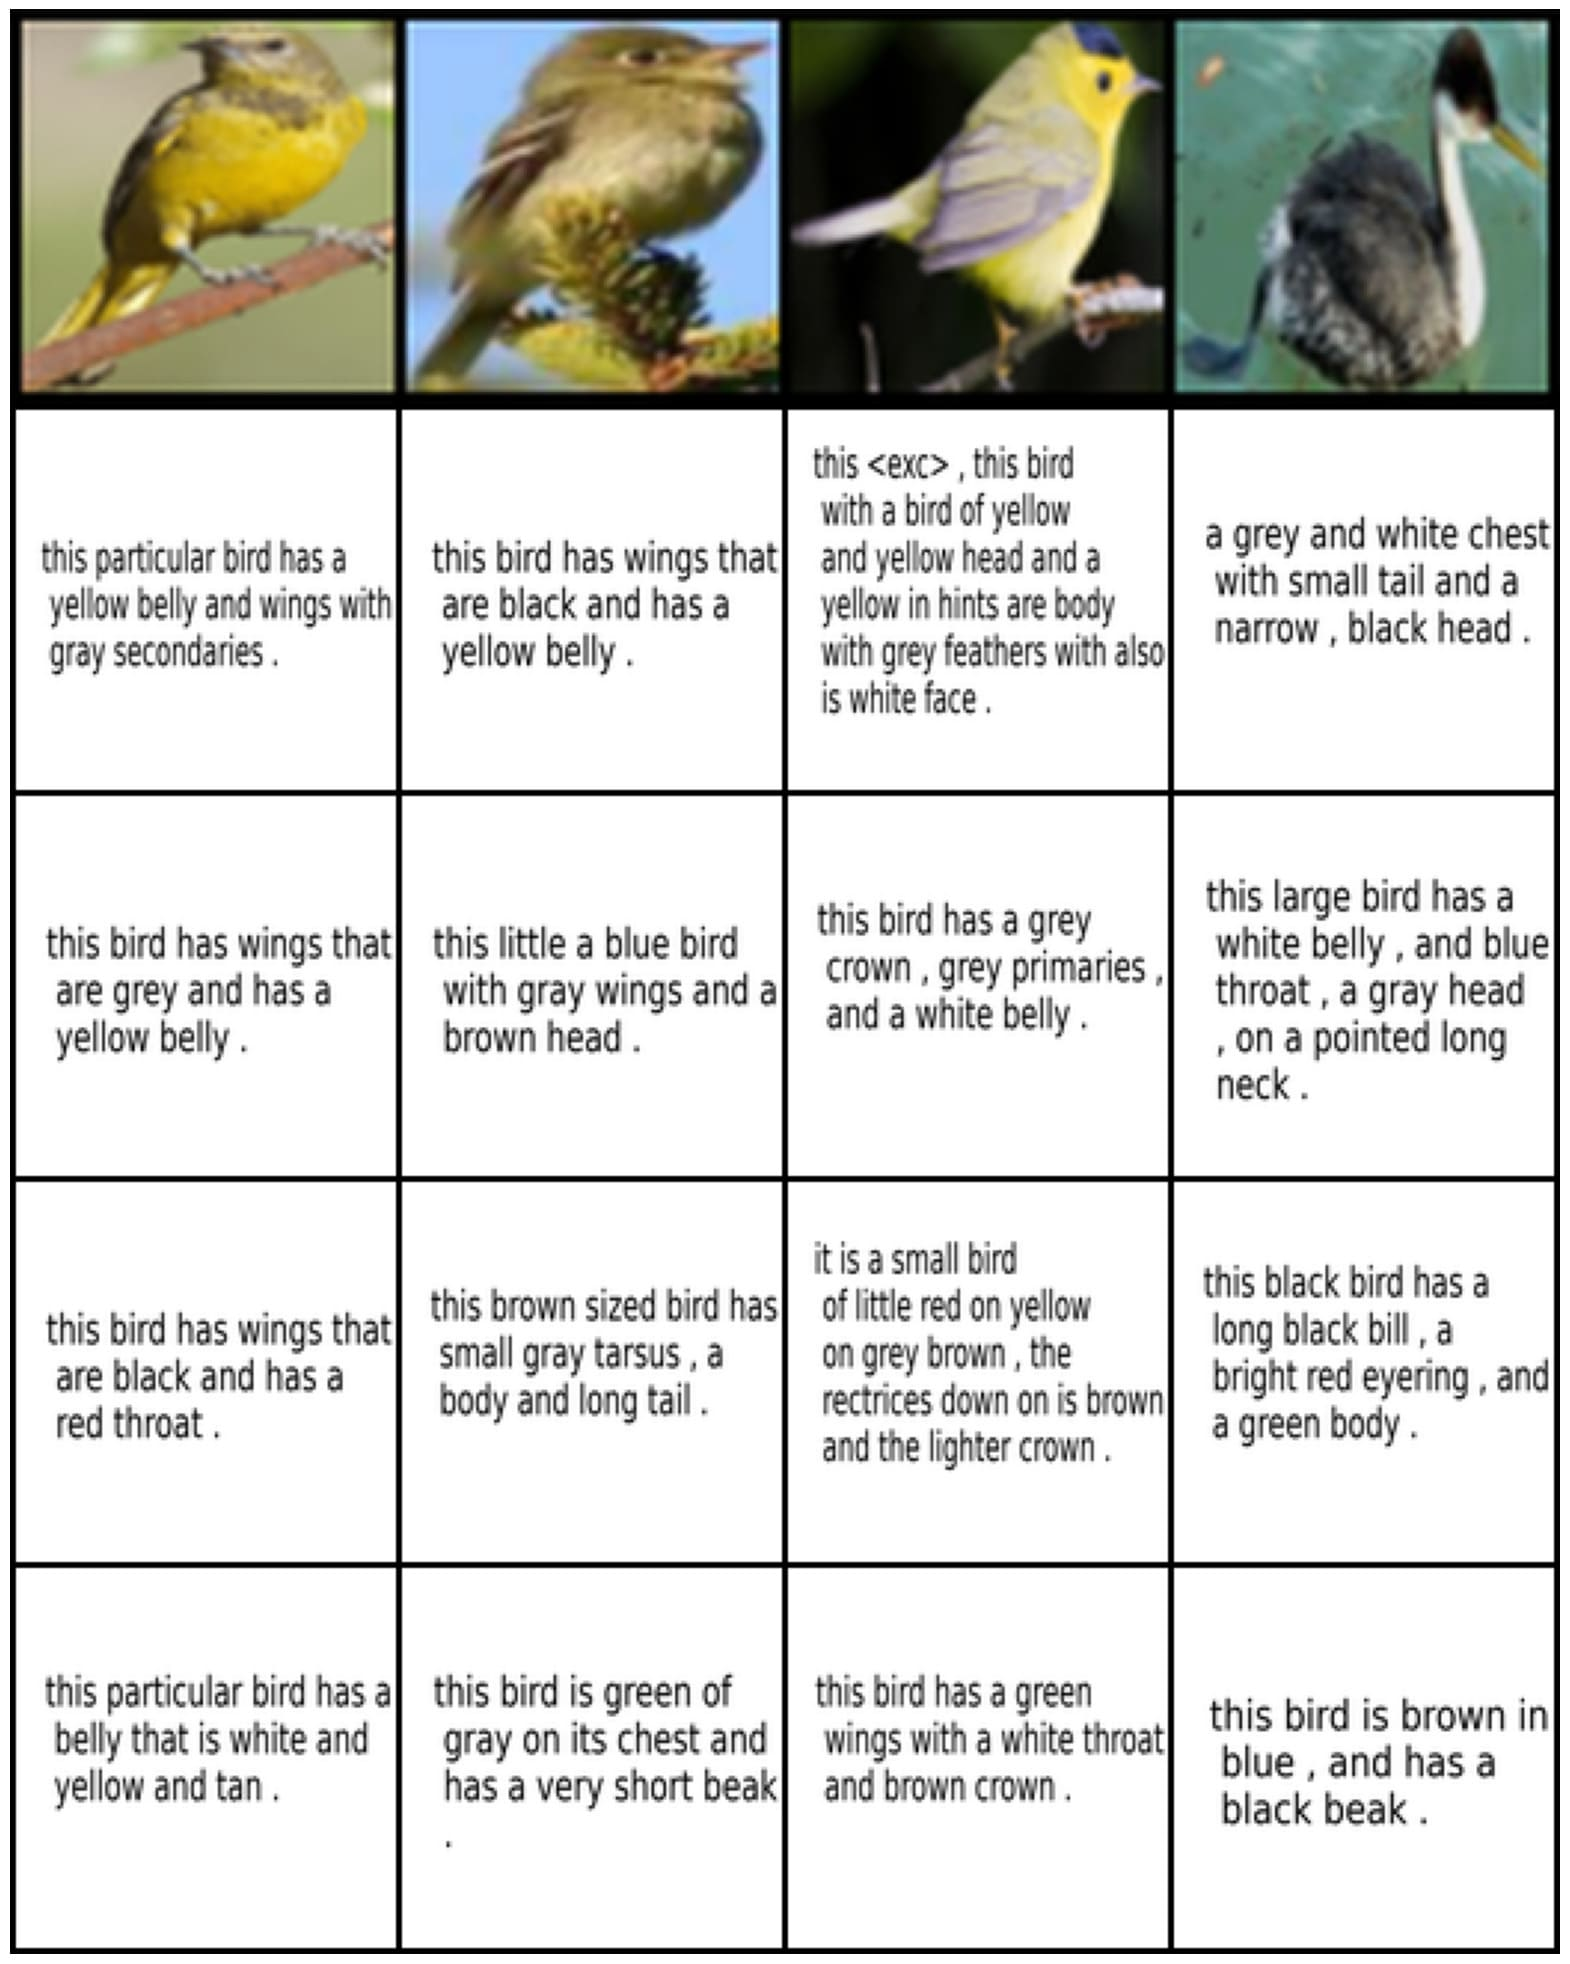
\includegraphics[page=1,width=\linewidth]{figures/datasets/cub/MLD_inpaint_cond_image_text}
%          \caption*{\gls{MLD Inpaint}  }
% \end{subfigure}

%  \begin{subfigure}{0.3\textwidth}
%          \centering
%          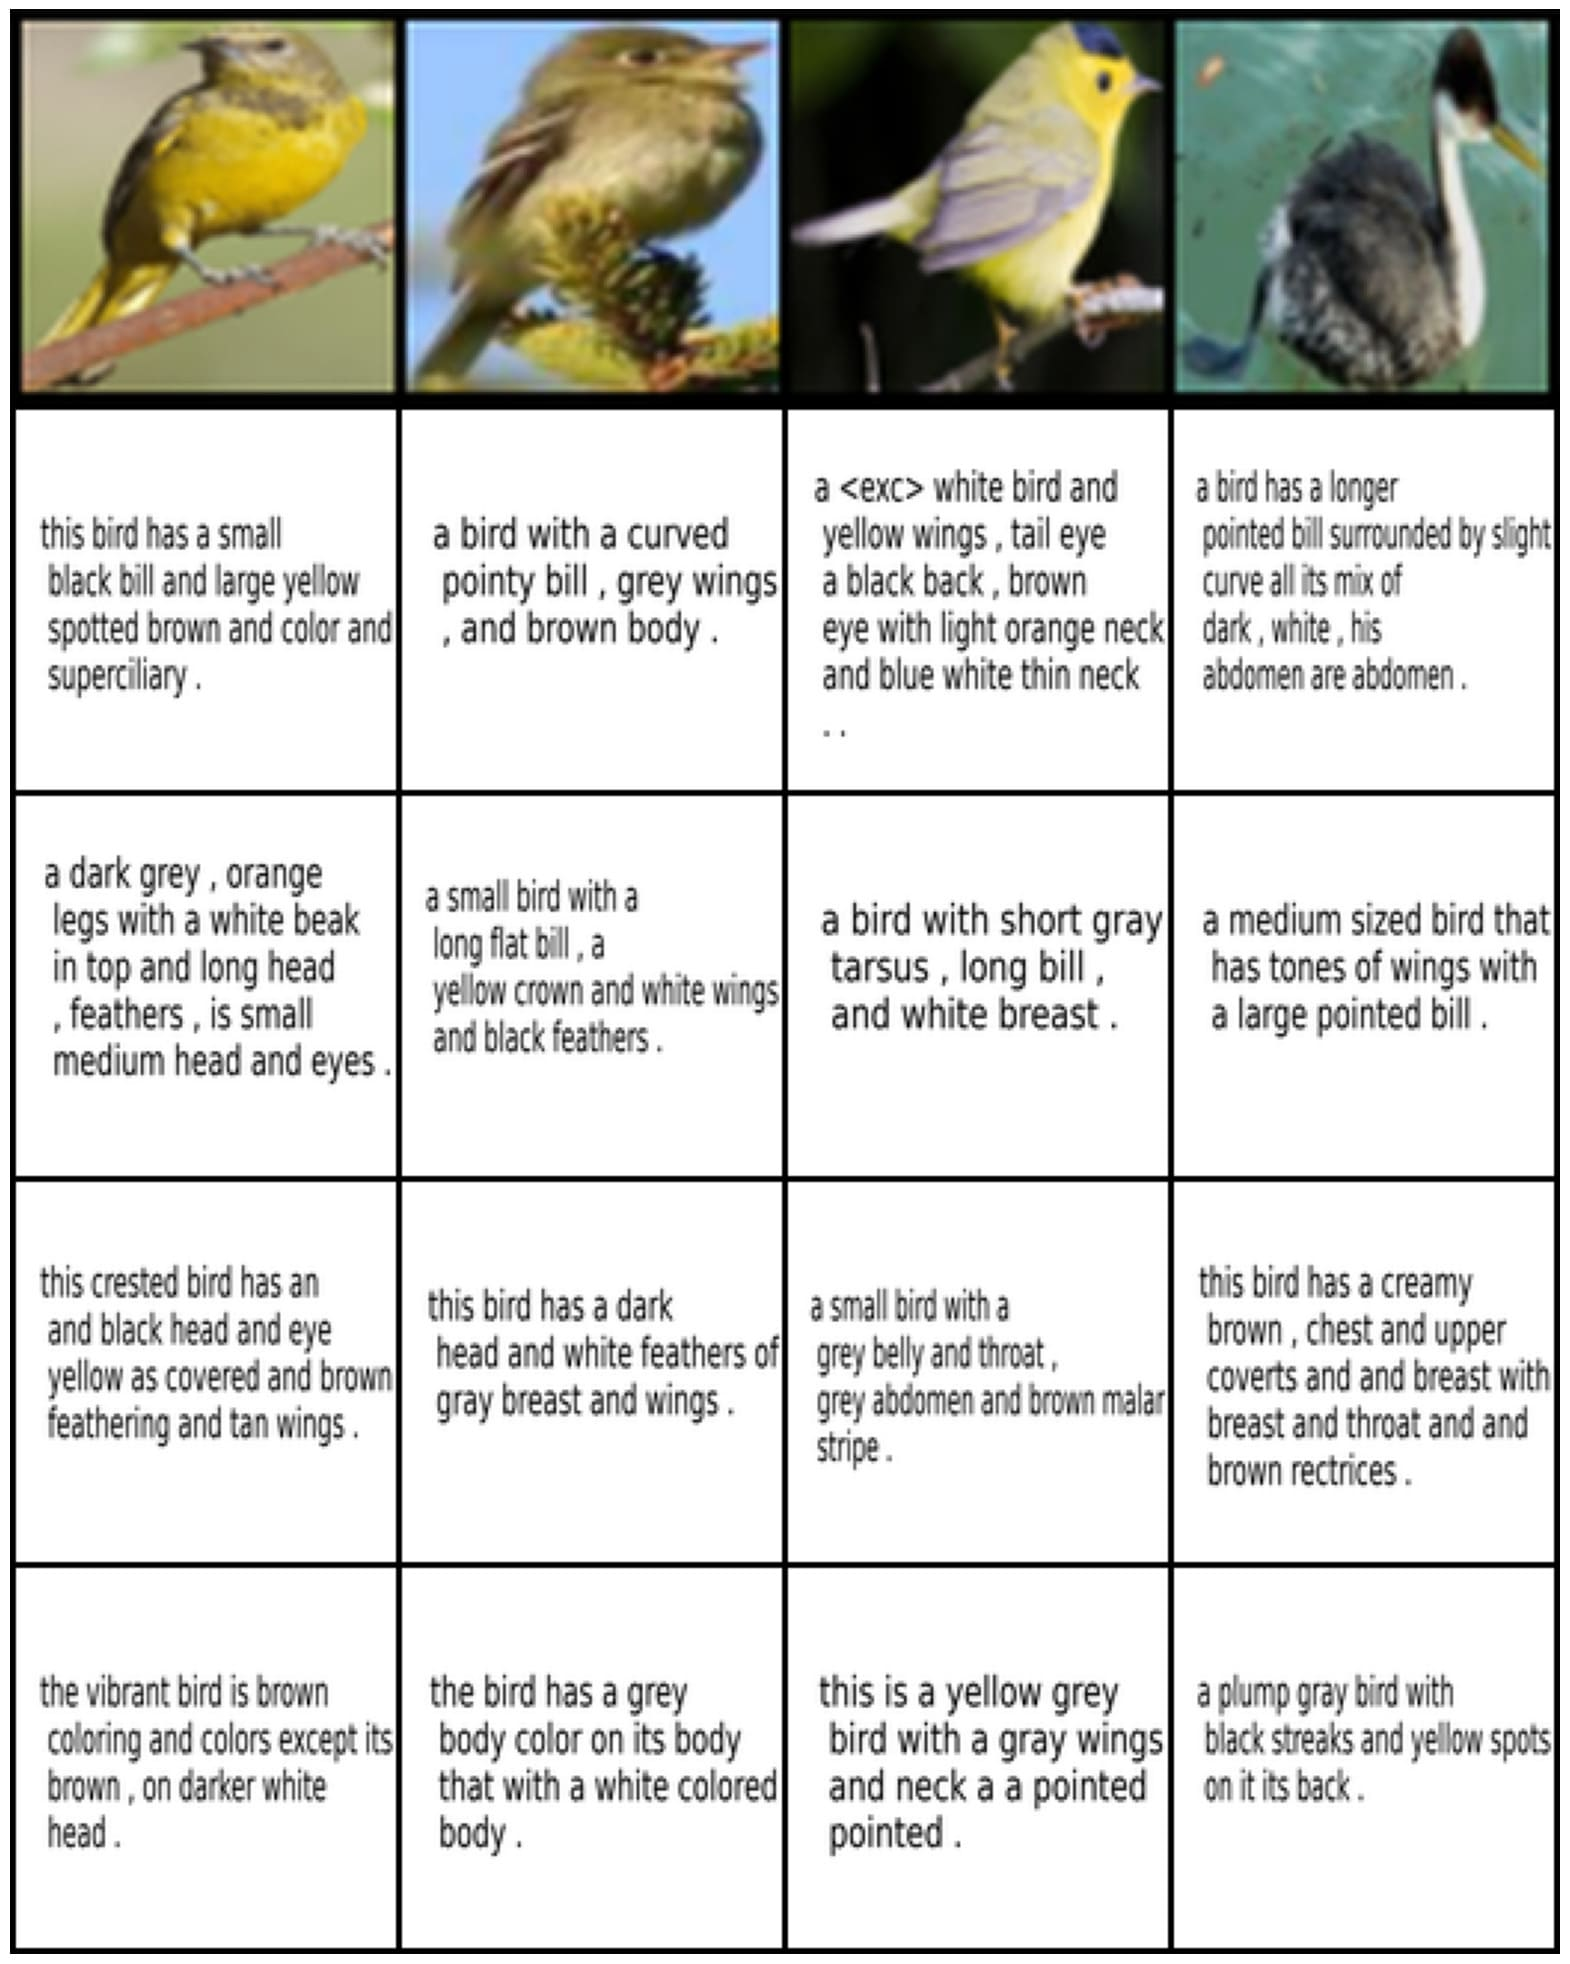
\includegraphics[page=1,width=\linewidth]{figures/datasets/cub/MLD_uni_cond_image_text}
%          \caption*{\gls{MLD Uni}  }
% \end{subfigure}
% \begin{subfigure}{0.3\textwidth}
%     \centering
%     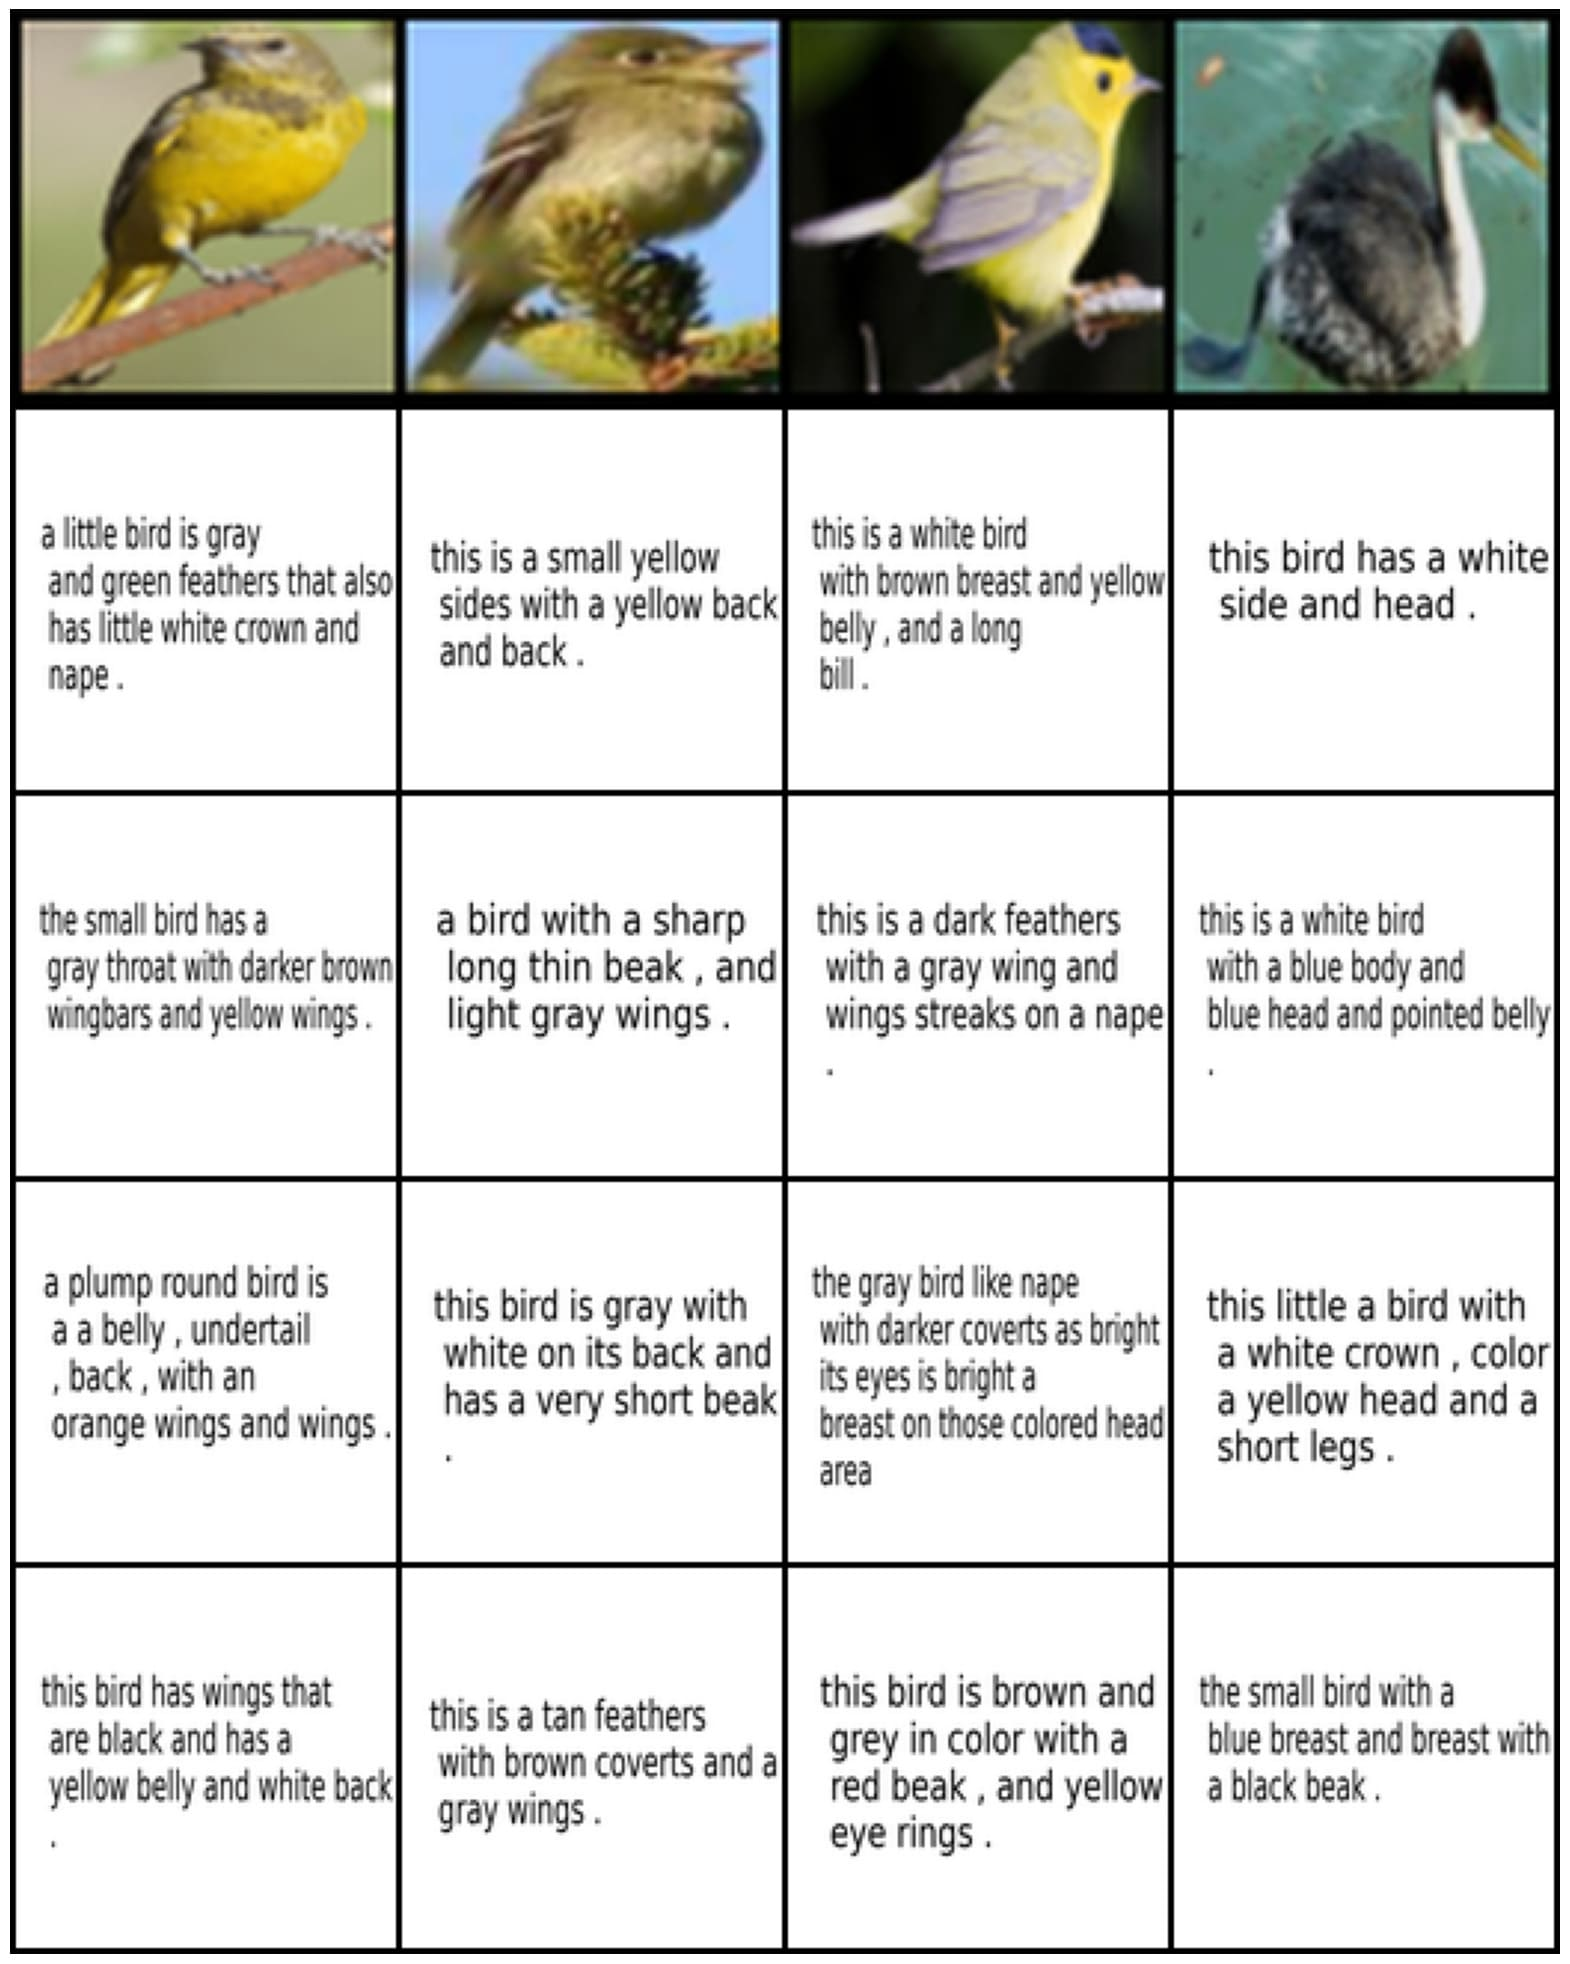
\includegraphics[page=1,width=\linewidth]{figures/datasets/cub/MLD_cond_image_text}
%     \caption*{\gls{MLD} (ours) }
% \end{subfigure}
% \caption{Qualitative results for Image to caption conditional generation  on \textbf{\cub}.}
% \label{cap_image_cub_detailed}
% \end{figure}


\begin{figure}[H]
     \centering
     
     \begin{subfigure}{0.25\textwidth}
         \centering
         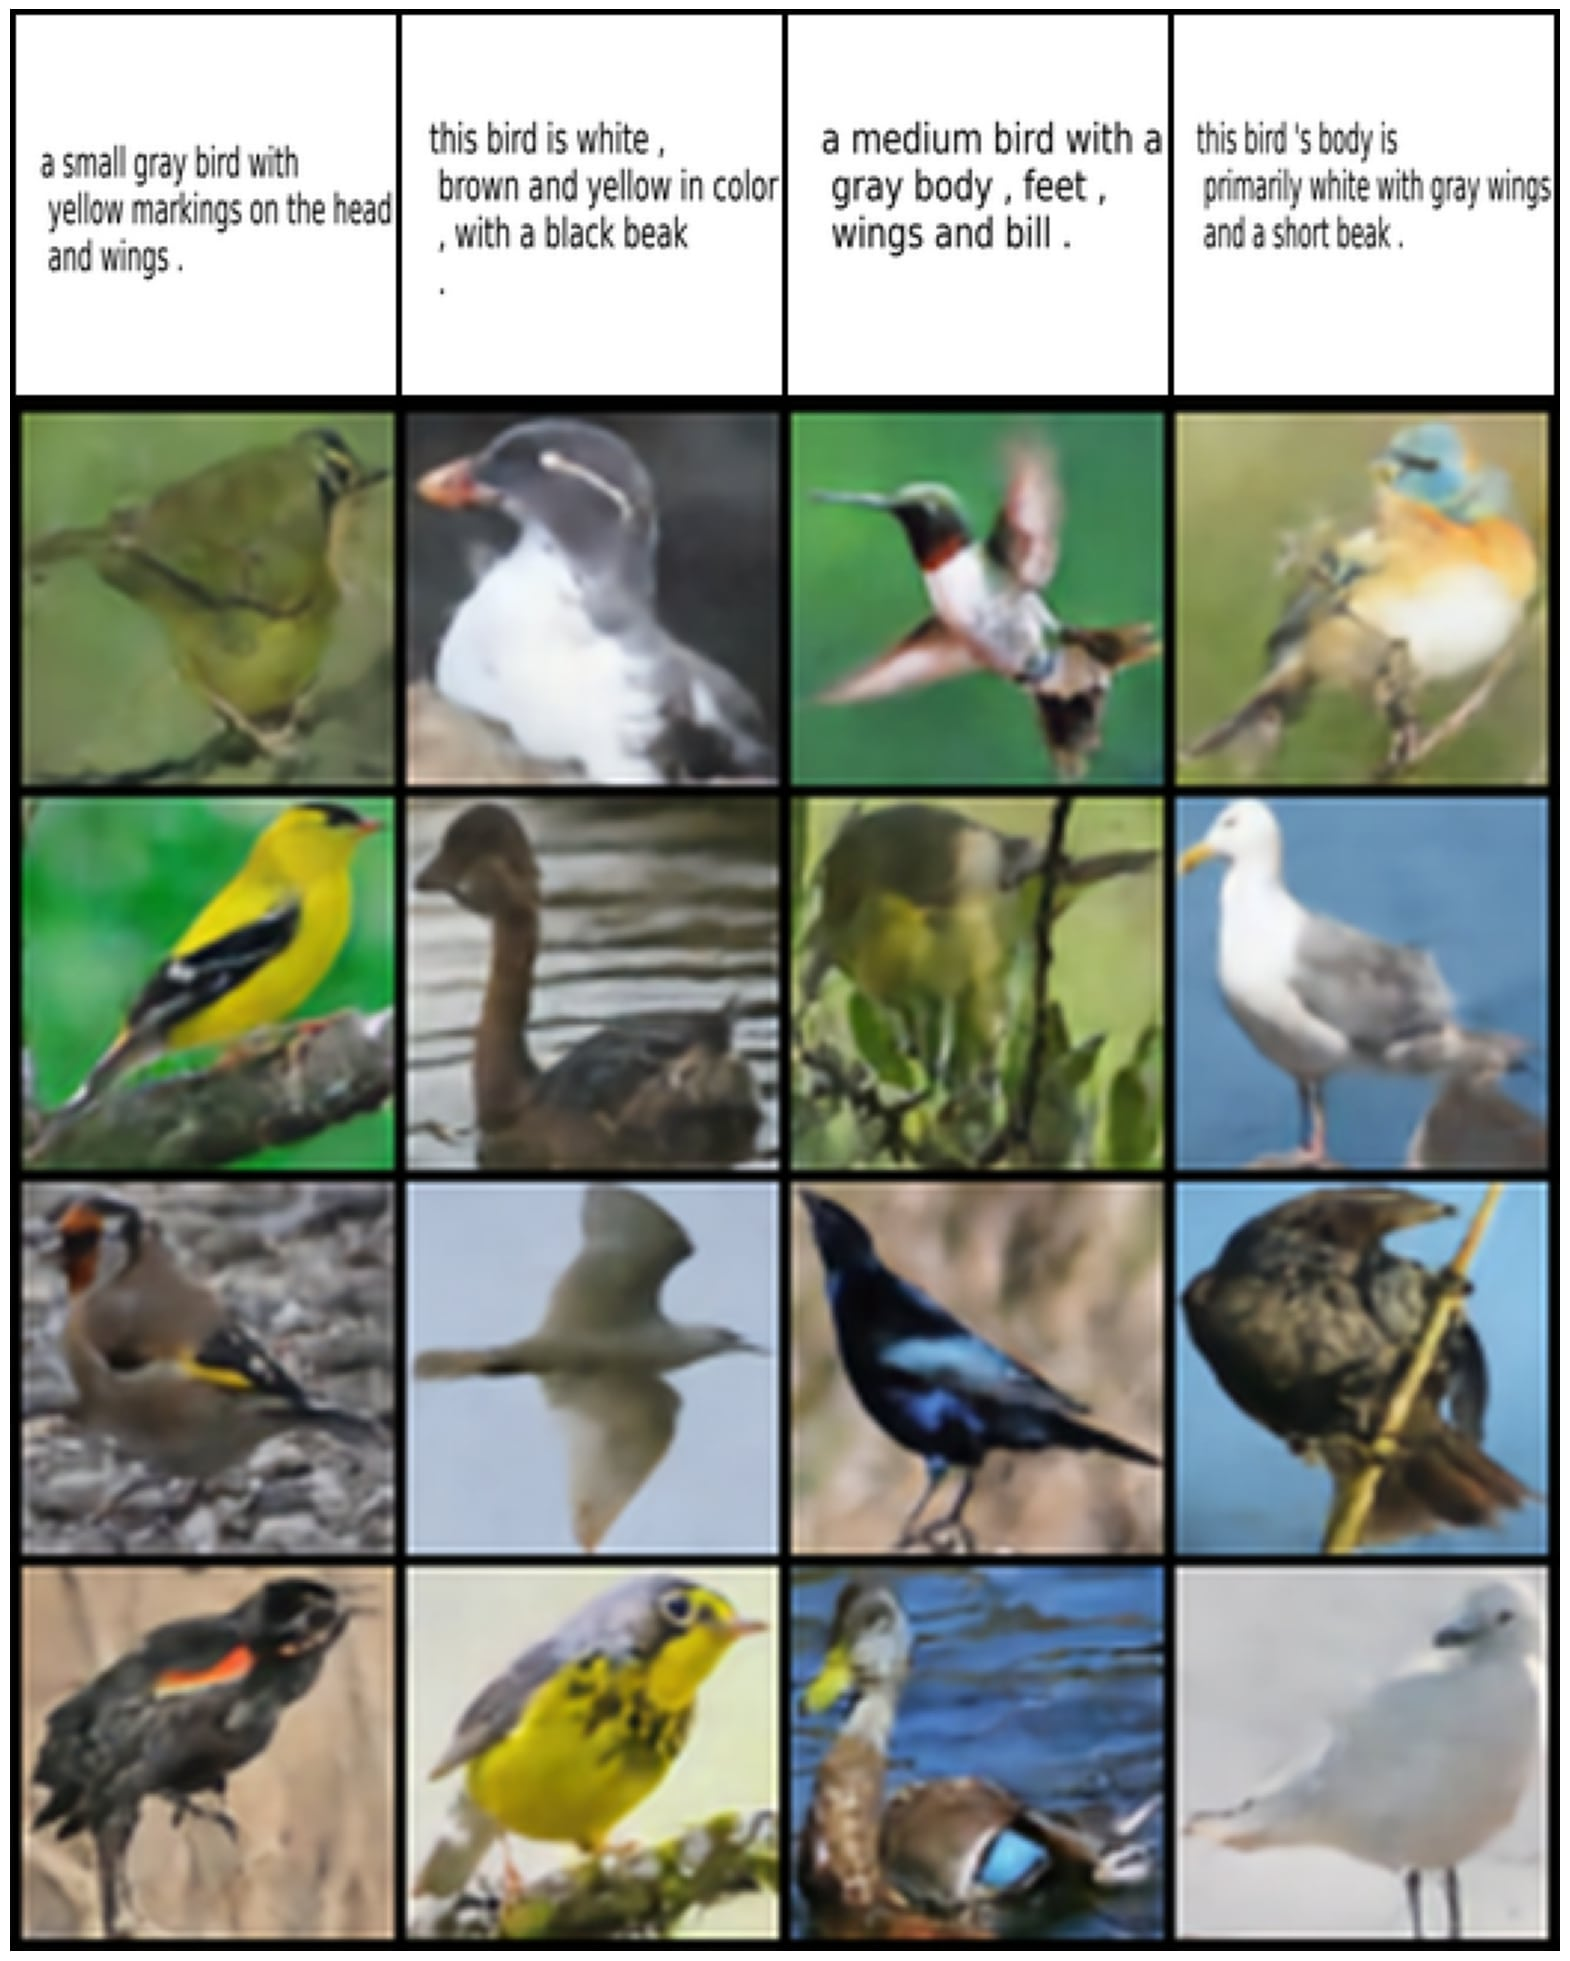
\includegraphics[width=\linewidth]{figures/datasets/cub/new_64/MLD_cond_text_image_mld64_new.jpg}
         \caption{ Conditional generation.}
    \end{subfigure}
  \begin{subfigure}{0.52\textwidth}
         \centering
         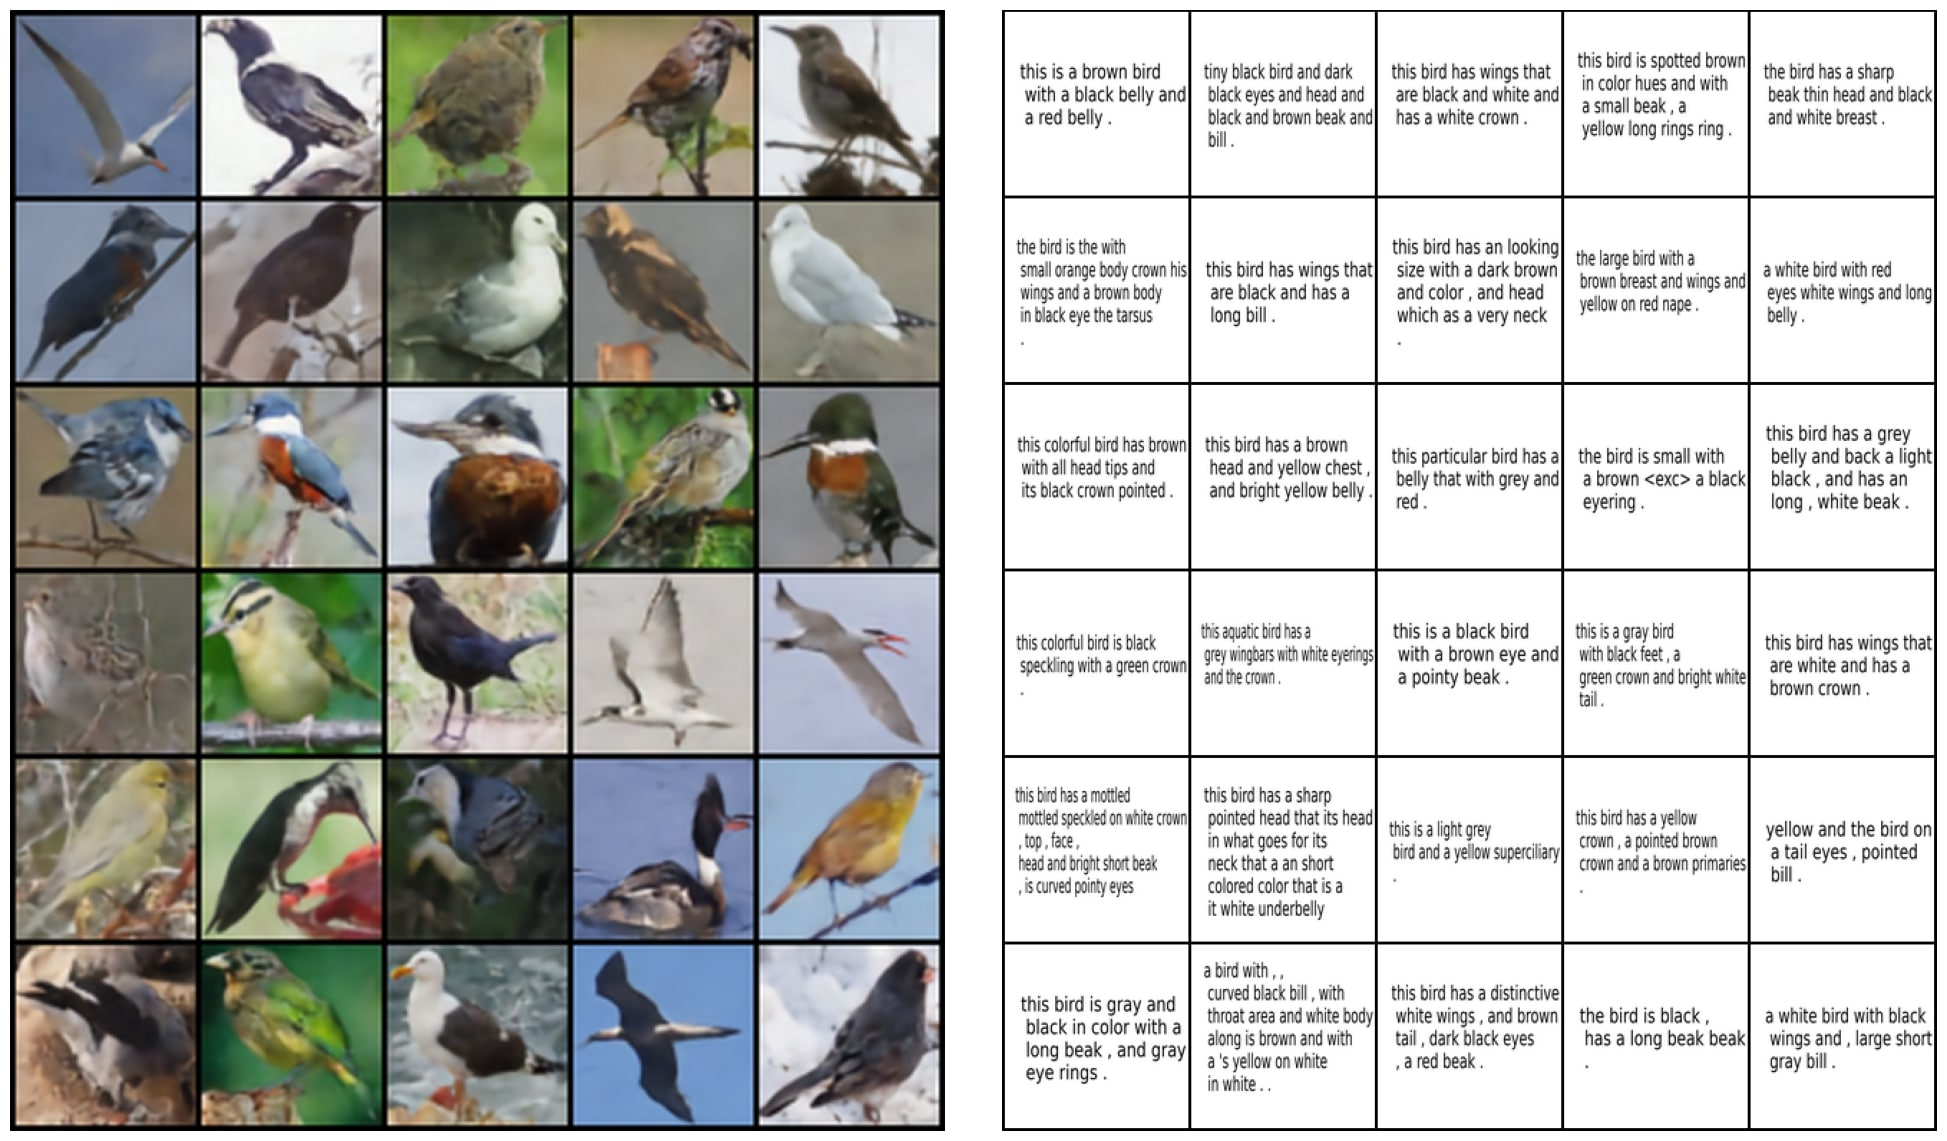
\includegraphics[width=\linewidth]{figures/datasets/cub/new_64/MLD_sampling64.jpg}
            \caption{Joint generation.}
         
\end{subfigure}
        \caption{Qualitative results of \textbf{\gls{MLD}*} on \textbf{CUB} data-set with powerful image autoencoder.}
    
\end{figure}



\begin{figure}[H]
     \centering
     \begin{subfigure}{0.30\textwidth}
         \centering
         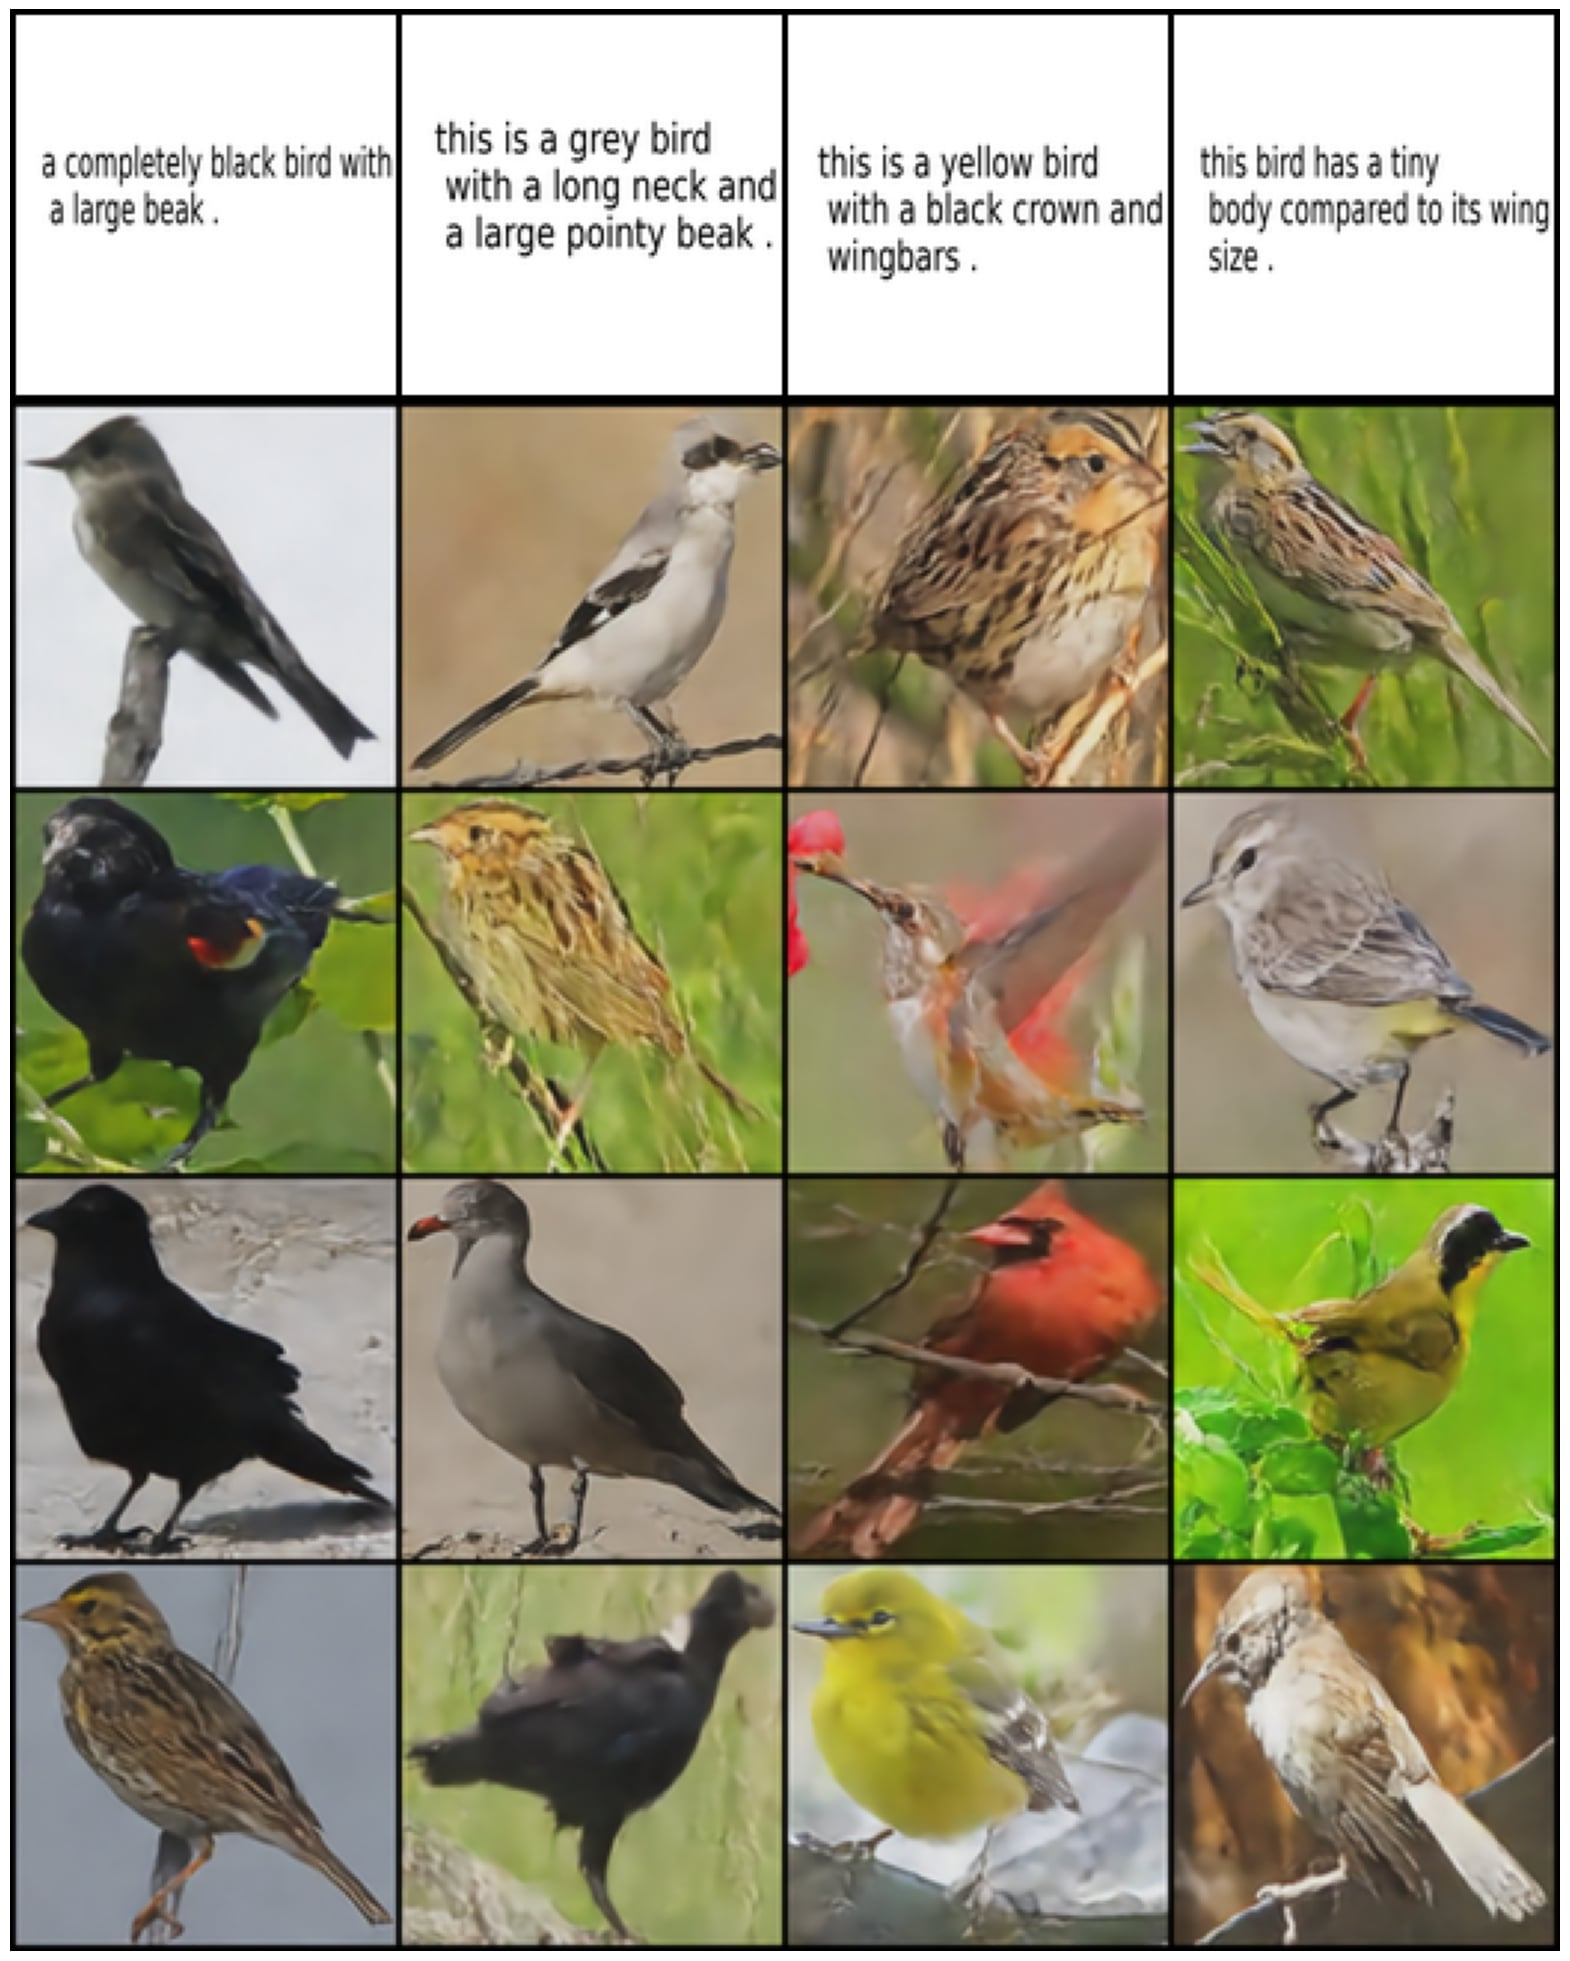
\includegraphics[width=\linewidth]{figures/datasets/cub/new_256/MLD_cond_text_image_mld_finalfinal.jpg}
          \caption{ Conditional Generation: Caption used as condition to generate the bird images.}
    \end{subfigure}
  \begin{subfigure}{0.69\textwidth}
         \centering
         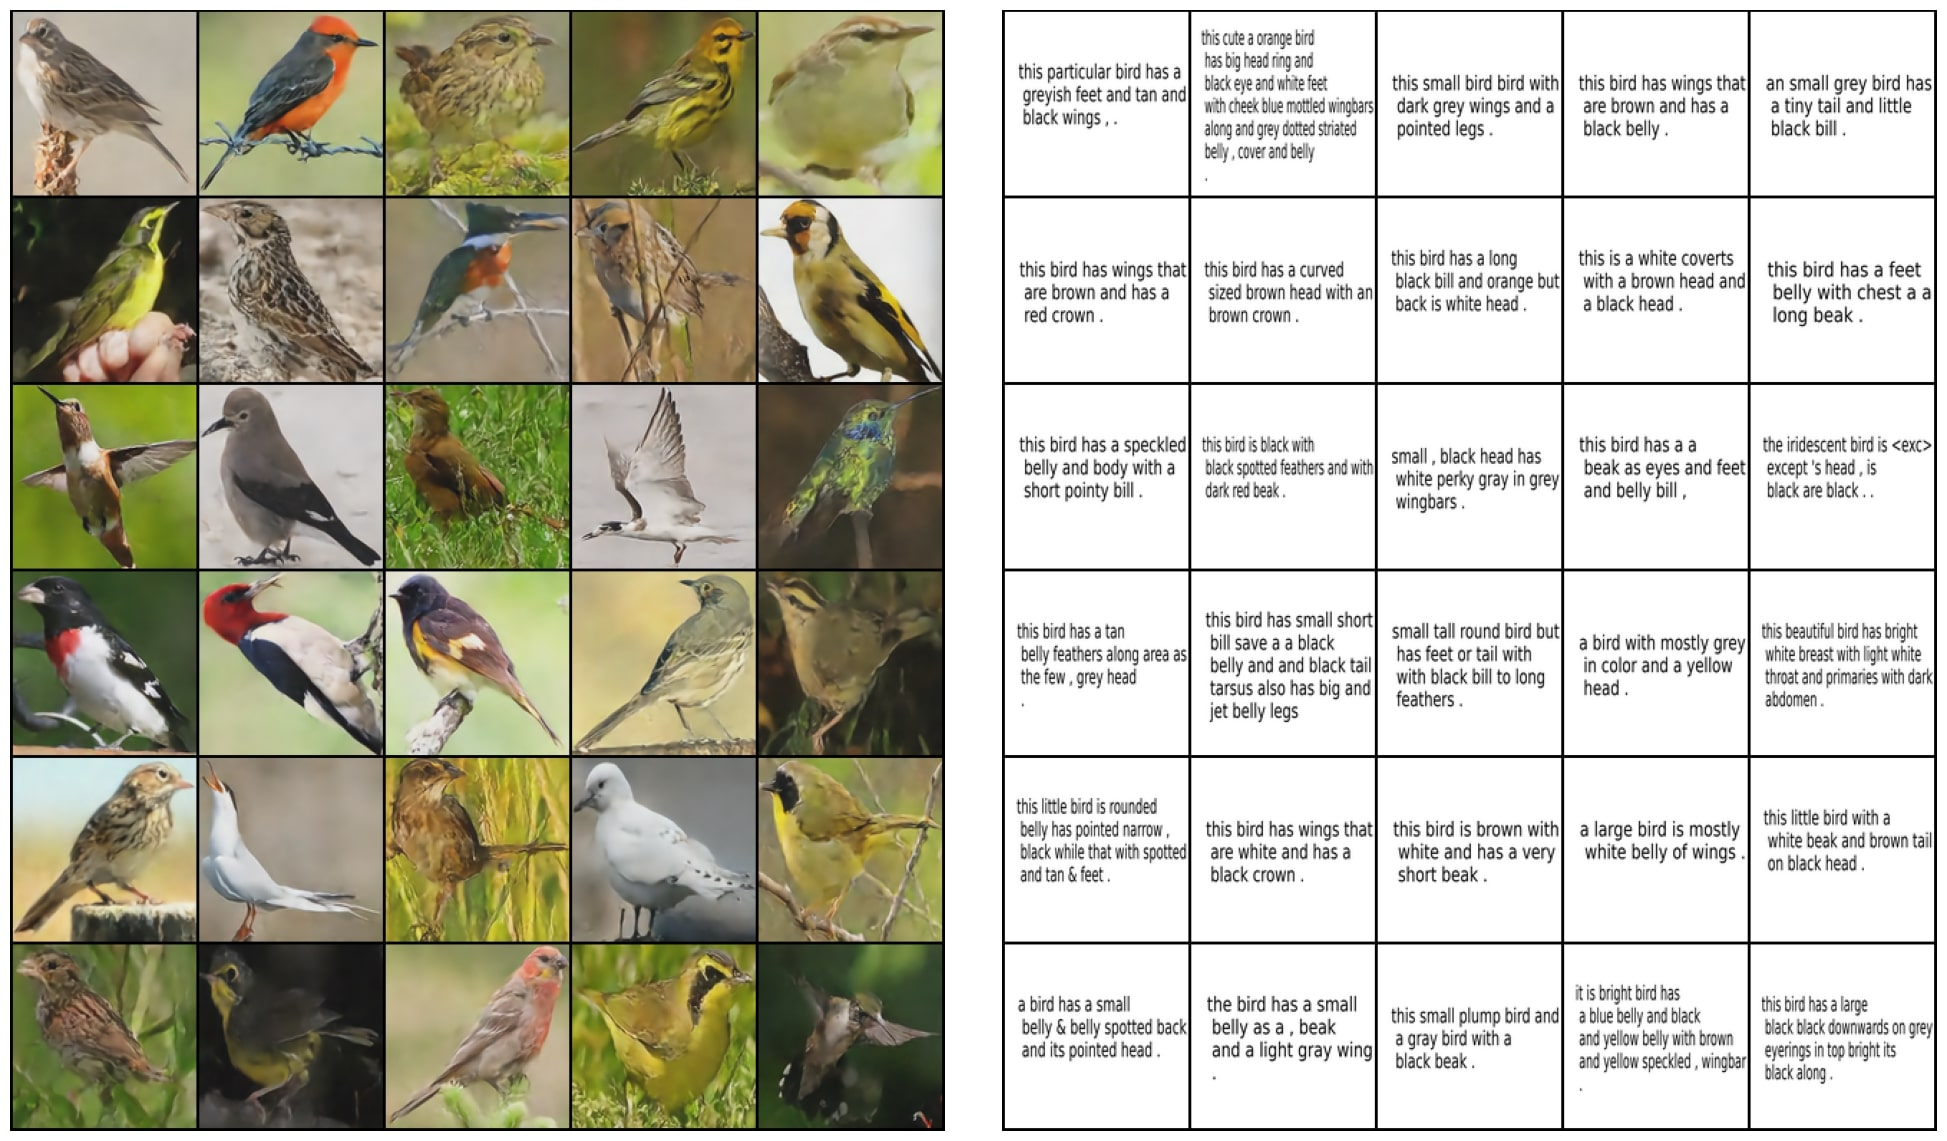
\includegraphics[width=\linewidth]{figures/datasets/cub/new_256/MLD_sampling_final.jpg}
         \caption{Joint generation: Images and captions are generated simultaneously.}
        
\end{subfigure}
    
        \caption{Qualitative results of \textbf{\gls{MLD}*} on \textbf{CUB} data-set with $128 $x$128$ resolution with powerful image autoencoder.
        }
       \label{cub128}
\end{figure}

\subsection{CelebAMask-HQ}

In this section, we present additional experiments on the CelebAMask-HQ dataset~\citep{Lee2019MaskGANTD}, which consists of face images, each having a segmentation mask, and text attributes, so 3 modalities. We follow the same experimentation protocol as in \citep{wesego2023scorebased} including the autoencoder base architecture. Note that for \gls{MLD} we use deterministic autoencoders instead of variational autoencoders~\citep{Lee2019MaskGANTD}.
Similarly, the CelebAMask-HQ dataset is restricted to take into account 18 out of 40 attributes from the original dataset and the images are resized to 128$\times$128 resolution, as done in~\citep{mvaeWu2018,wesego2023scorebased}. Please refer to \Cref{apdx:implementation}, for additional implementation details of \gls{MLD}.

The Image generation quality is evaluated in terms of \gls{FID} score. The attributes and the mask having binary values, are evaluated in terms of $F1$ Score against the ground truth. The competitors performance results are reported from~\cite{wesego2023scorebased}. 

The quantitative results in \Cref{coh_qua:celebA} show that \gls{MLD} outperforms the competitors on the generation quality. It achieves the best F1 score in the attributes generation given Image and Mask modalities. The mask generation best performance is achieved by \gls{MOPOE}. \gls{MLD} achieves the second best performance on the mask generation conditioning on both image and attributes modalities. Overall, \gls{MLD} stands out with the best image quality generation while being on-par with competitors in the mask and attribute generation coherence.








\begin{figure}[H]
     \centering
     
     \begin{subfigure}{0.49\textwidth}
         \centering
         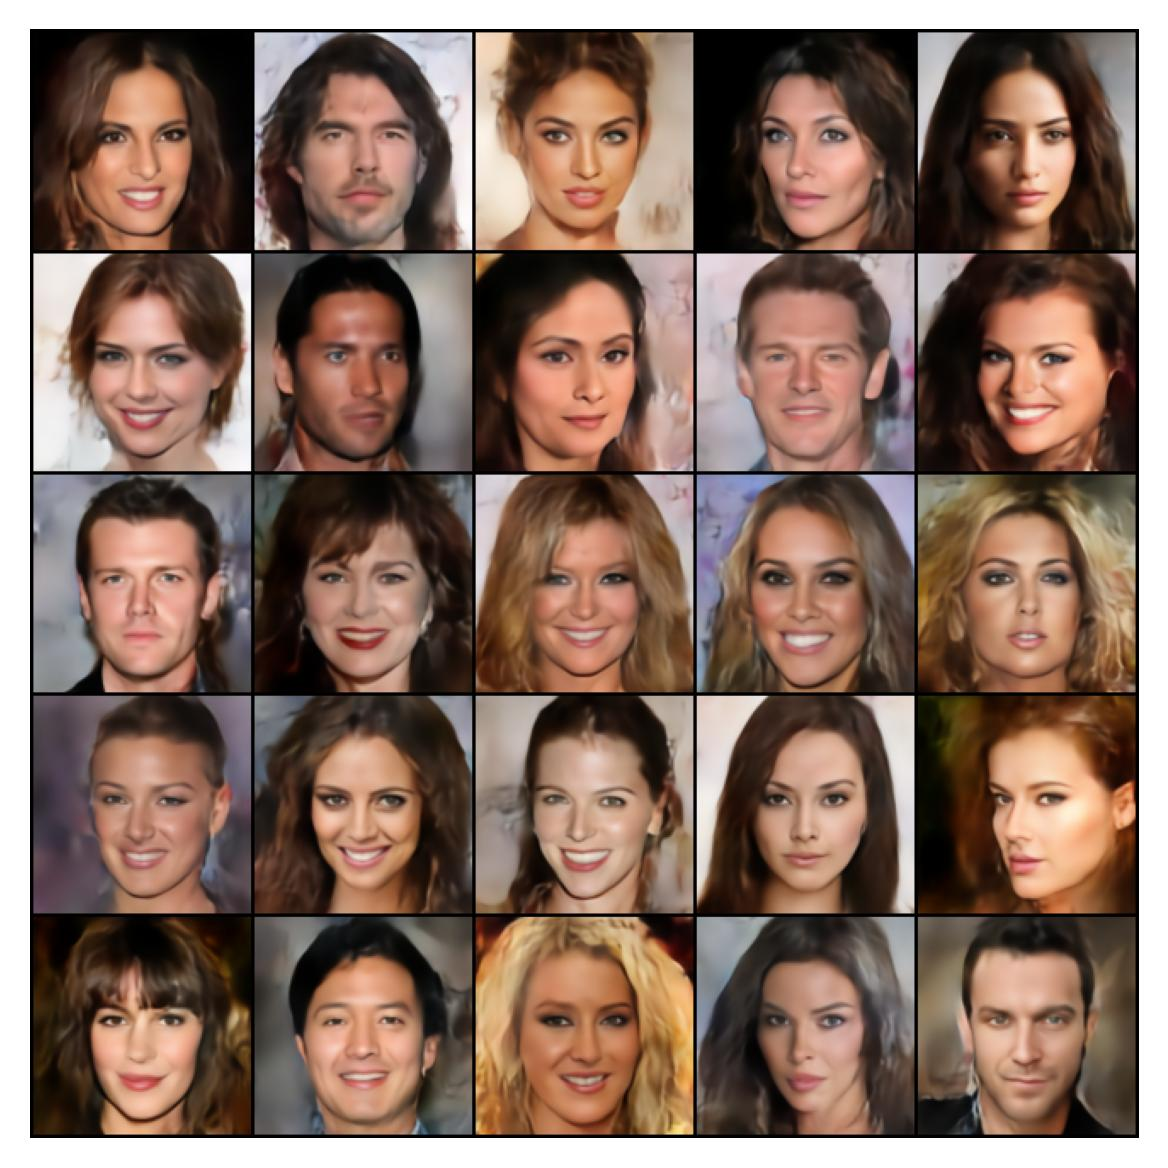
\includegraphics[width=\linewidth]{figures/datasets/celebA/image_joint.jpg}
         \caption{Image}
    \end{subfigure}
  \begin{subfigure}{0.49\textwidth}
         \centering
         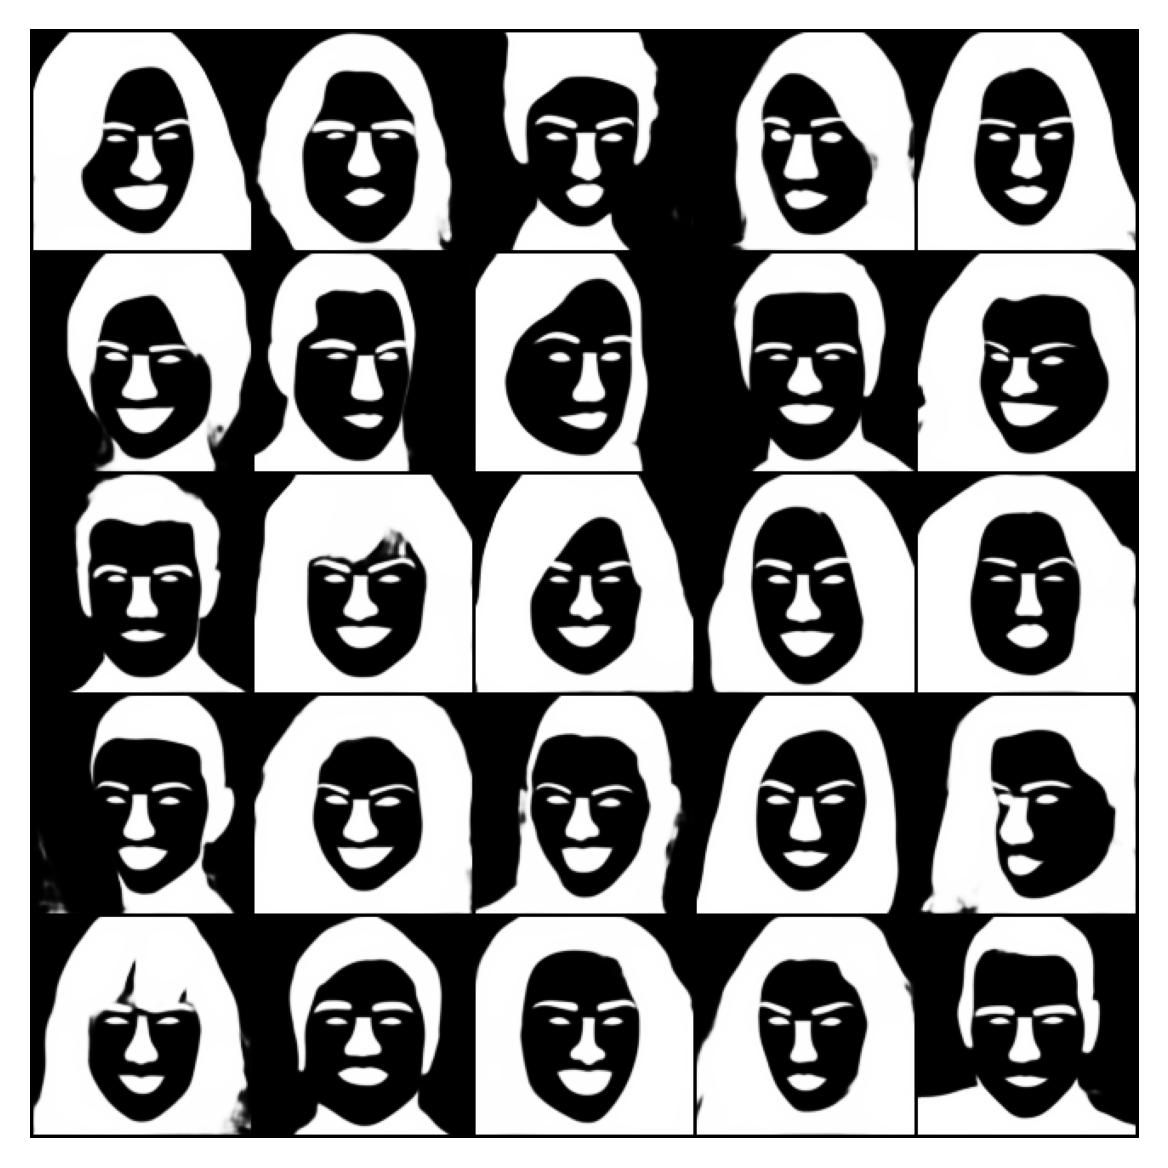
\includegraphics[width=\linewidth]{figures/datasets/celebA/mask_joint.jpg}
            \caption{Mask}
\end{subfigure}
  \begin{subfigure}{0.49\textwidth}
         \centering
         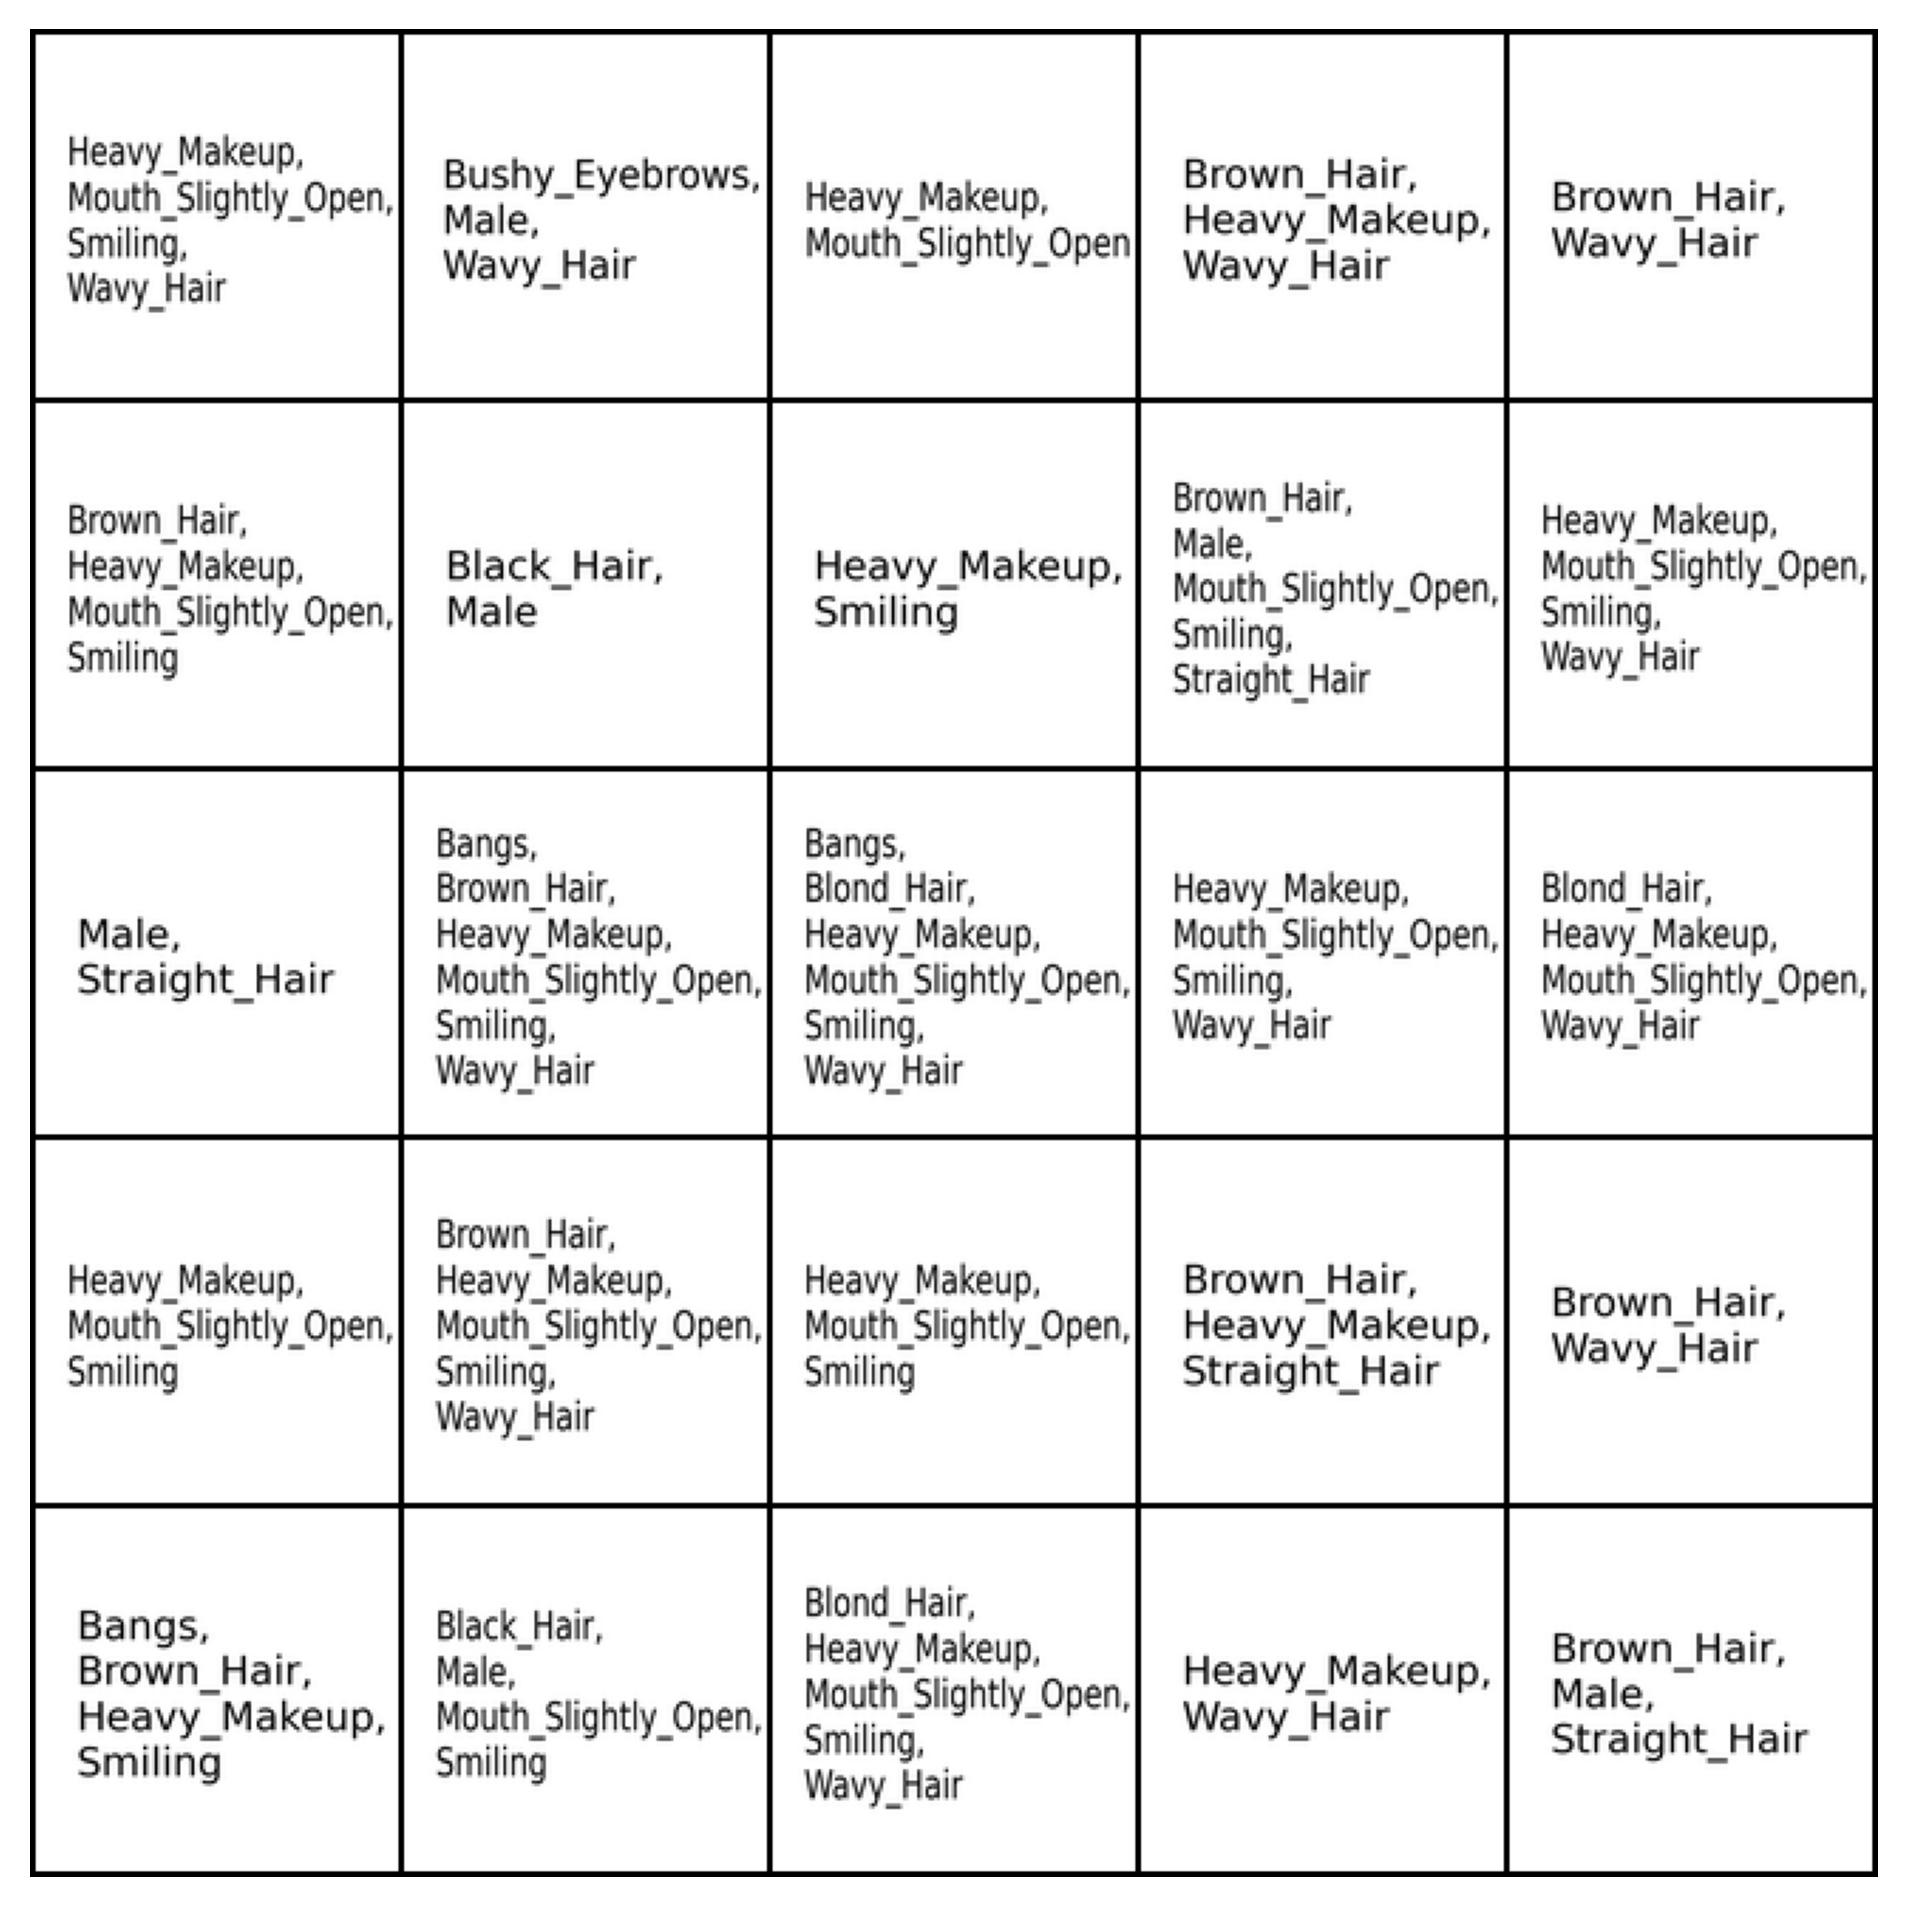
\includegraphics[width=\linewidth]{figures/datasets/celebA/attributes_joint.jpg}
            \caption{Attributes}
\end{subfigure}
        \caption{Joint (Unconditional) generation  qualitative results of \textbf{\gls{MLD}} on CelebAMask-HQ.}
    
       
\end{figure}





\begin{table}[H]
\tiny
\centering
\begin{tabular}{c|cc|cccc|cc}
\toprule
\multirow{3}{*}{ Models }  & \multicolumn{2}{c}{ Attributes }  &  \multicolumn{4}{c}{Image }  &  \multicolumn{2}{c}{Mask } \\
    \cmidrule{2-9}
    &  Img + Mask & Img &  Att + Mask & Mask  & Att & Joint & Img+Att & Img \\
   
    &  F1 & F1 &  FID  & FID  & FID & FID & F1  & F1 \\
     \midrule
     \\
     \cite{wesego2023scorebased} 
     \\
     SBM-RAE  & 0.62 & 0.6 & 84.9& 86.4 & 85.6& 84.2 & 0.83 & 0.82
    \\
     SBM-RAE-C & 0.66 & 0.64& 83.6& 82.8& 83.1& 84.2 & 0.83 & 0.82
     \\
     SBM-VAE& 0.62 & 0.58 & 81.6& 81.9 & 78.7&79.1& 0.83 & 0.83
     \\
     SBM-VAE-C& 0.69 & 0.66 & 82.4& 81.7 & 76.3& 79.1 & 0.84 & 0.84

     \\
          \cmidrule{2-9}
     \gls{MOPOE} & 0.68 & \textbf{0.71} &114.9 & 101.1 &186.8 & 164.8 & 0.85 & \textbf{0.92}
     \\
      \gls{MVTCAE} & 0.71 & 0.69 & 94 & 84.2 &87.2 & 162.2 &\textbf{0.89} & 0.89
      \\
    \gls{MMVAEplus} & 0.64 & 0.61 &133 & 97.3 & 153 &103.7 & 0.82 & 0.89 \\
     \midrule
   Supervised classifier &   &
   0.79  & &  &   &  & 0.94 \\
  \midrule
\textbf{ \gls{MLD} (ours) } & 
 $ \textbf{0.72}$&
 $0.69$ &

 $\textbf{52.75}$ & 
    $\textbf{51.73}$ & 
    $\textbf{53.09}$ &
 $\textbf{54.27}$ 
 & 0.87 & 0.87 \\
    \bottomrule

\end{tabular}
\caption{Quantitative results on CelebAMask-HQ dataset. The performance is measured in terms of \gls{FID} ($ \downarrow $) and F1 score ($ \uparrow $). The first row is the generated modality while the second row is the modalities used as condition.
Supervised classifier designates a classifier performance to predict the attributes or the mask from an image. }
\label{coh_qua:celebA}

 \end{table}



 


\begin{figure}[H]
     \centering
     
     \begin{subfigure}{0.14\textwidth}
                \begin{subfigure}{1\textwidth}
    
         
\includegraphics[width=\linewidth]{figures/datasets/celebA/examp2/2_attributes_c.jpg}
         \caption*{ }
          \end{subfigure}

                    \begin{subfigure}{1\textwidth}
    
         
\includegraphics[width=\linewidth]{figures/datasets/celebA/examp3/3_attributes_c.jpg}
         \caption*{ }
          \end{subfigure}

              \begin{subfigure}{1\textwidth}
    
         
\includegraphics[width=\linewidth]{figures/datasets/celebA/examp4/4_attributes_c.jpg}
         \caption*{ }
          \end{subfigure}

            
          
    \end{subfigure}
  \begin{subfigure}{0.14\textwidth}


\end{subfigure}
  \begin{subfigure}{0.7\textwidth}
  
     \begin{subfigure}{1\textwidth}
      
         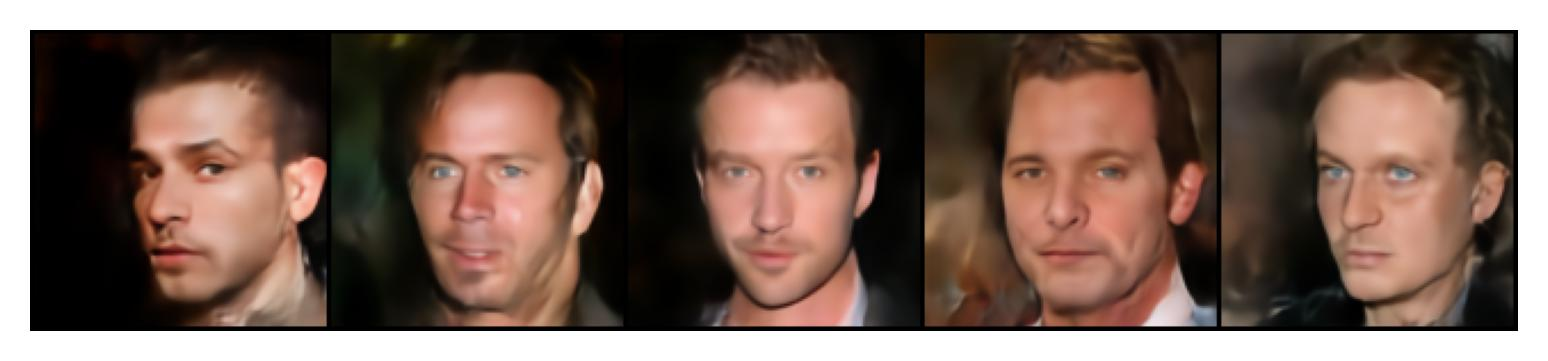
\includegraphics[width=\linewidth]{figures/datasets/celebA/examp2/2_im_cond_attr.jpg}
    \end{subfigure}

        \begin{subfigure}{1\textwidth}
      
         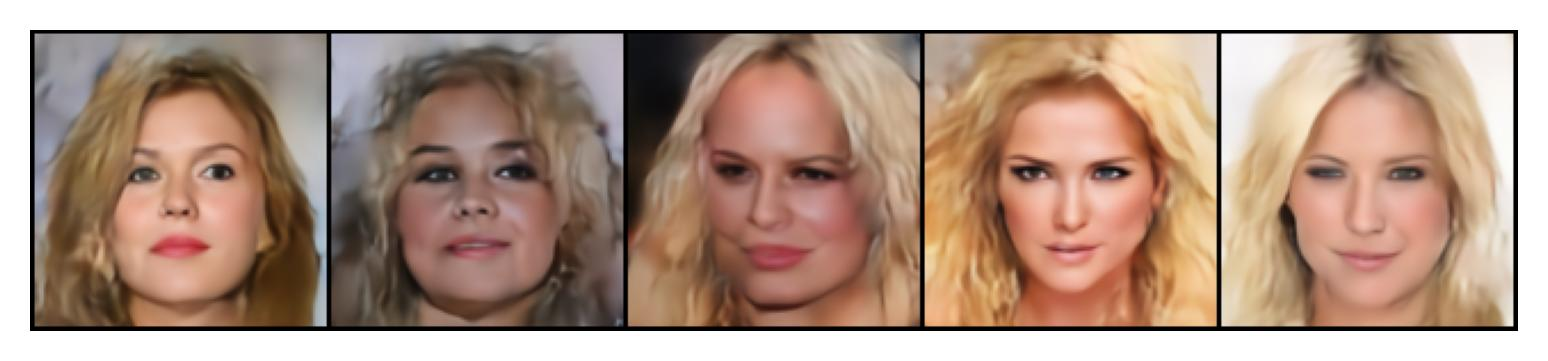
\includegraphics[width=\linewidth]{figures/datasets/celebA/examp3/3_im_cond_att.jpg}
    \end{subfigure}
    
      \begin{subfigure}{1\textwidth}
         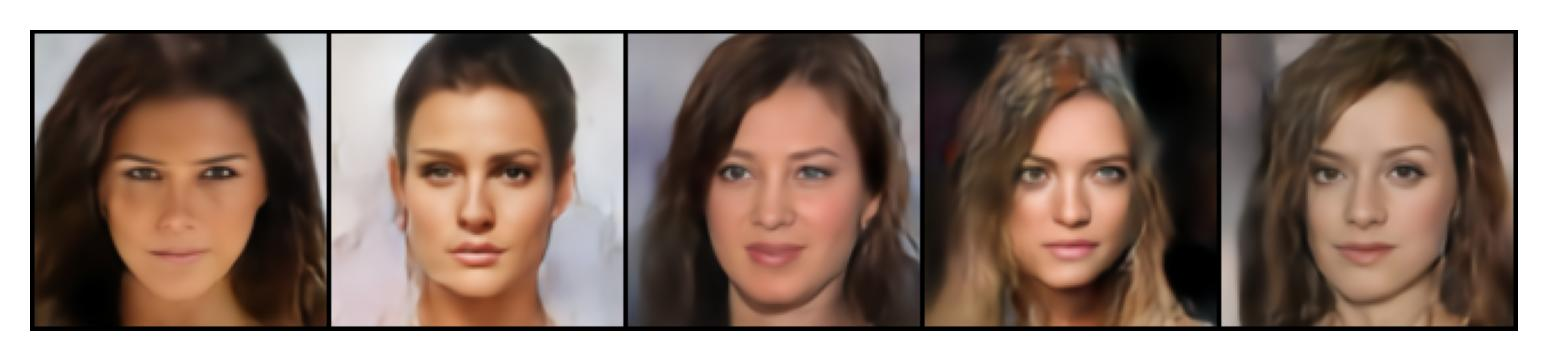
\includegraphics[width=\linewidth]{figures/datasets/celebA/examp4/4_im_cond_attr.jpg}
    \end{subfigure}

        
          
            \caption{Generated Images}
\end{subfigure}
        \caption{ (Attributes $\rightarrow$ Image ) Conditional generation of \textbf{\gls{MLD}} on CelebAMask-HQ.}

       
\end{figure}





\begin{figure}[H]
     \centering
     
     \begin{subfigure}{0.13\textwidth}

      \begin{subfigure}{1\textwidth}
     
         
\includegraphics[width=\linewidth]{figures/datasets/celebA/attributes_c_1.jpg}
     \caption*{ }
          \end{subfigure}
          
                \begin{subfigure}{1\textwidth}
    
         
\includegraphics[width=\linewidth]{figures/datasets/celebA/examp2/2_attributes_c.jpg}
  \caption*{ }
          \end{subfigure}
         %  \begin{subfigure}{1\textwidth}
         % \includegraphics[width=\linewidth]{figures/datasets/celebA/examp3/3_attributes_c.jpg
         %  \end{subfigure}
              \begin{subfigure}{1\textwidth}
     
         
\includegraphics[width=\linewidth]{figures/datasets/celebA/examp4/4_attributes_c.jpg}
 \caption*{ }
          \end{subfigure}


                \begin{subfigure}{1\textwidth}
     
         
\includegraphics[width=\linewidth]{figures/datasets/celebA/examp5/5_attributes_c.jpg}
 \caption*{ }
          \end{subfigure}
          
    \end{subfigure}
  \begin{subfigure}{0.14\textwidth}
  
   \begin{subfigure}{1\textwidth}

         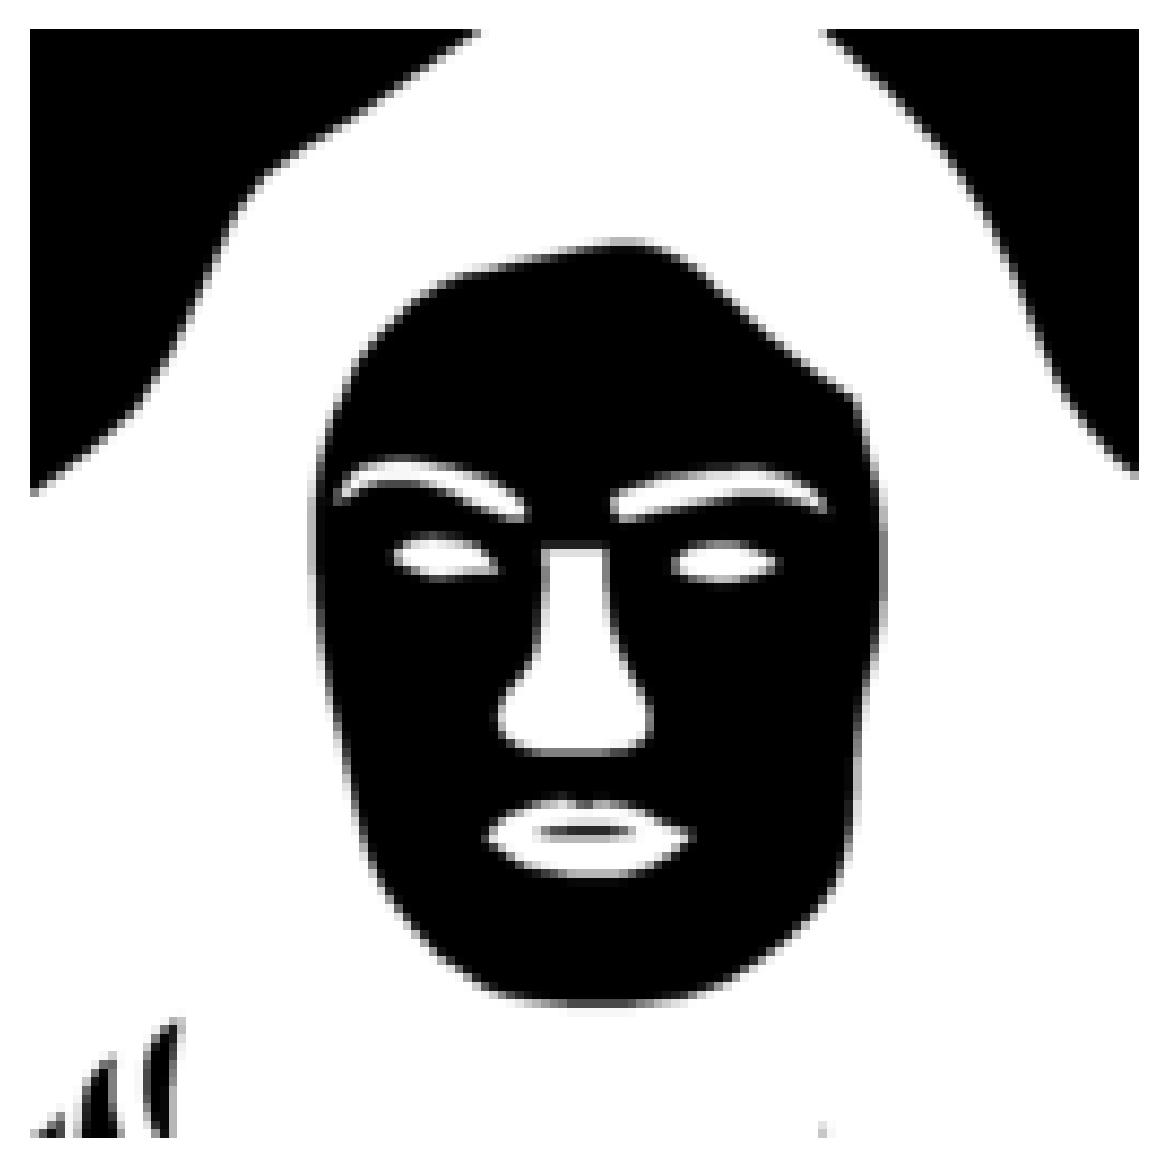
\includegraphics[width=\linewidth]{figures/datasets/celebA/mask_c_1.jpg}
        
    \end{subfigure}

      \begin{subfigure}{1\textwidth}
         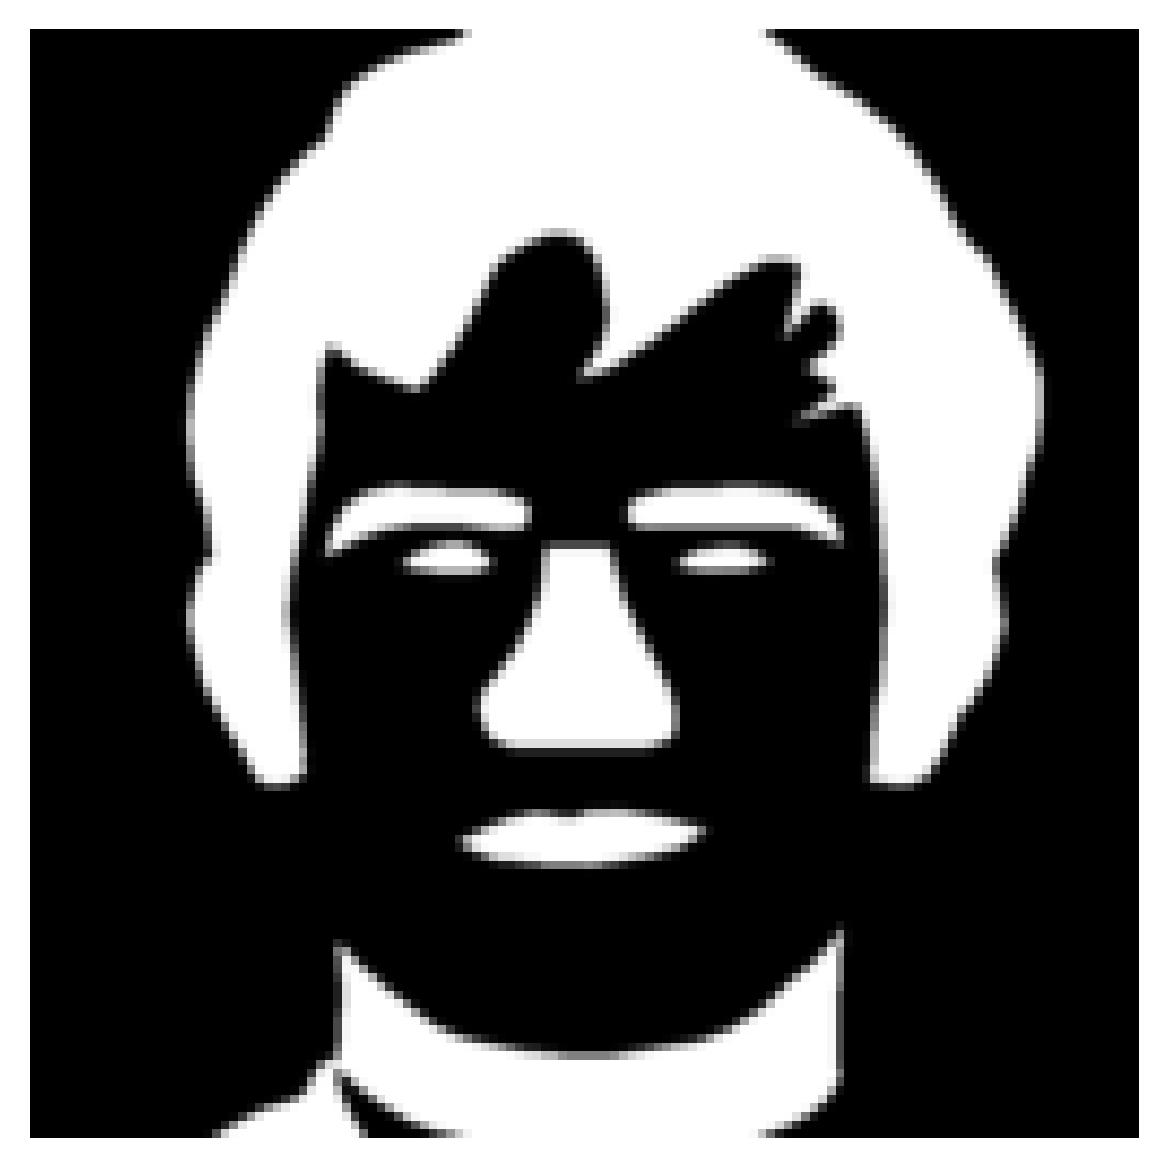
\includegraphics[width=\linewidth]{figures/datasets/celebA/examp2/2_mask_c.jpg}
    \end{subfigure}
    
     % \begin{subfigure}{1\textwidth}
     
     %     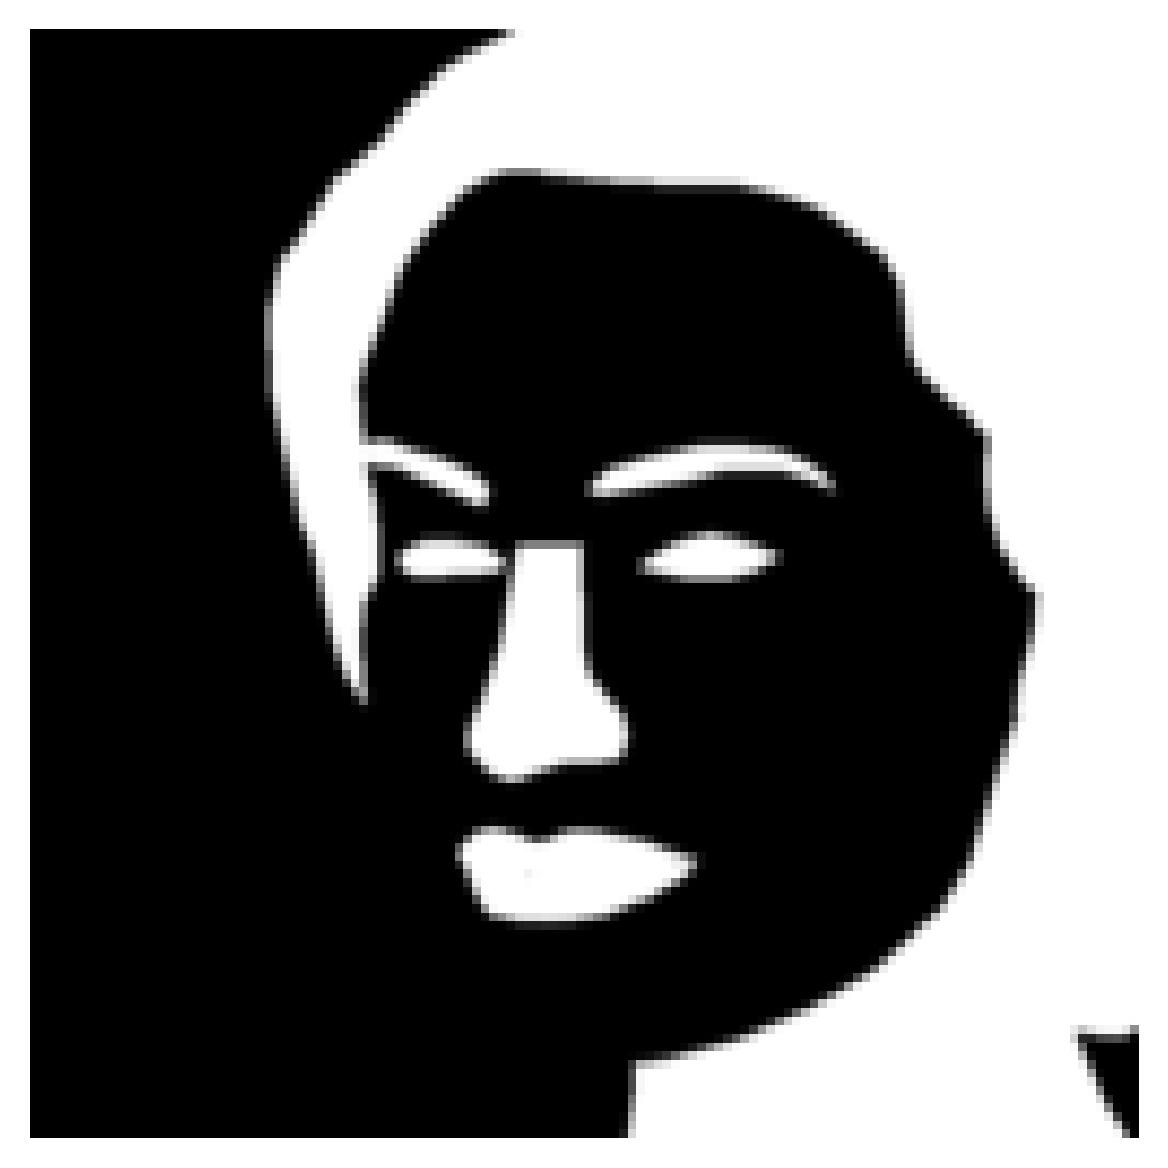
\includegraphics[width=\linewidth]{figures/datasets/celebA/examp3/3_mask_c.jpg}
     %     \caption*{ }
     %      \end{subfigure}

               \begin{subfigure}{1\textwidth}
     
         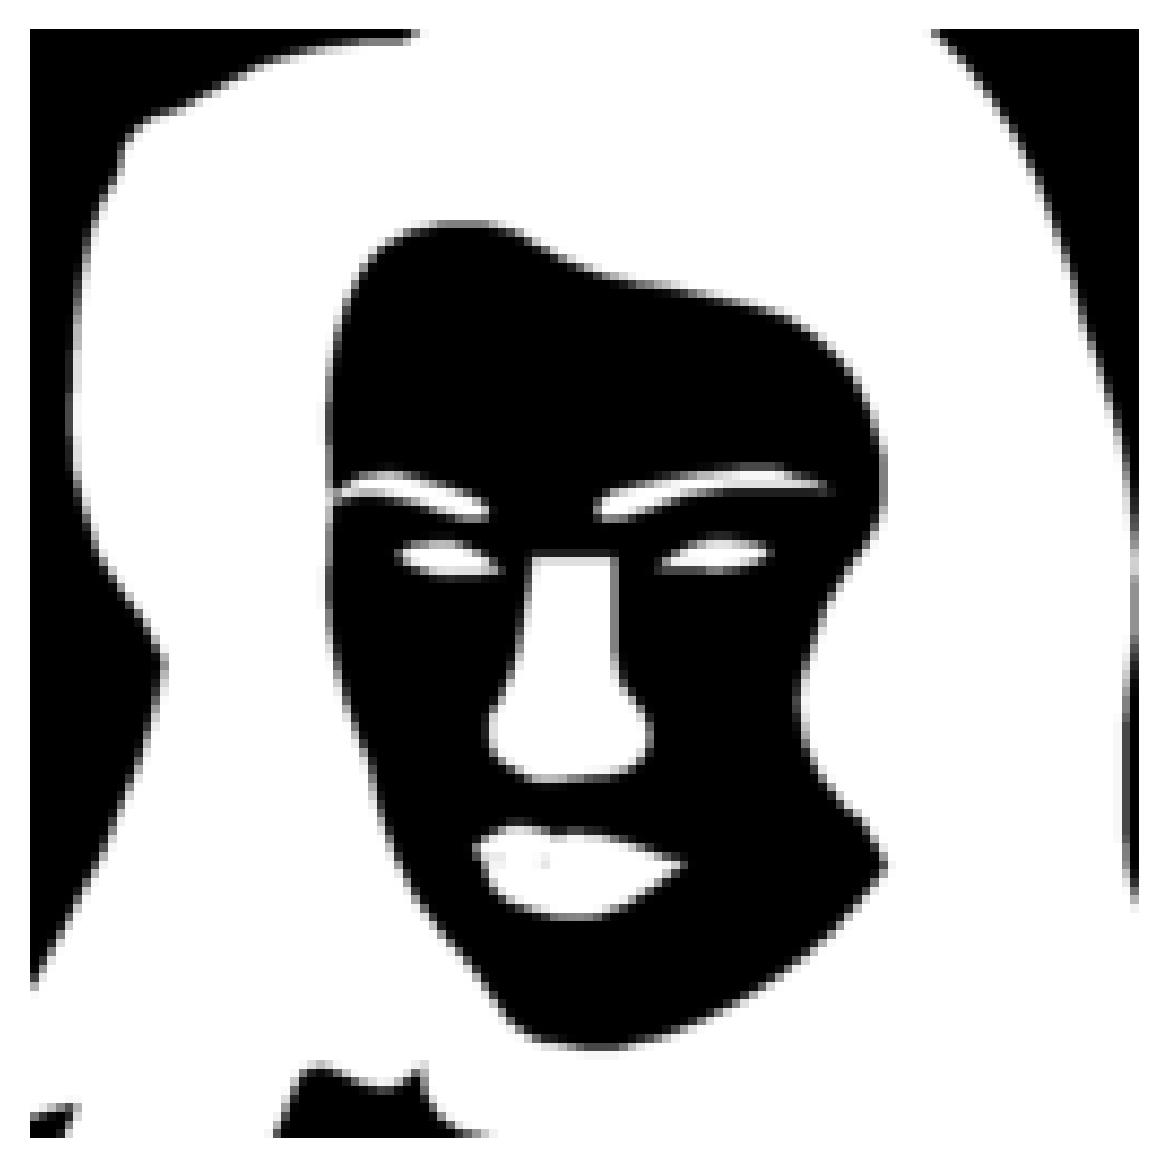
\includegraphics[width=\linewidth]{figures/datasets/celebA/examp4/4_mask_c.jpg}
         \caption*{ }
          \end{subfigure}

             \begin{subfigure}{1\textwidth}
     
         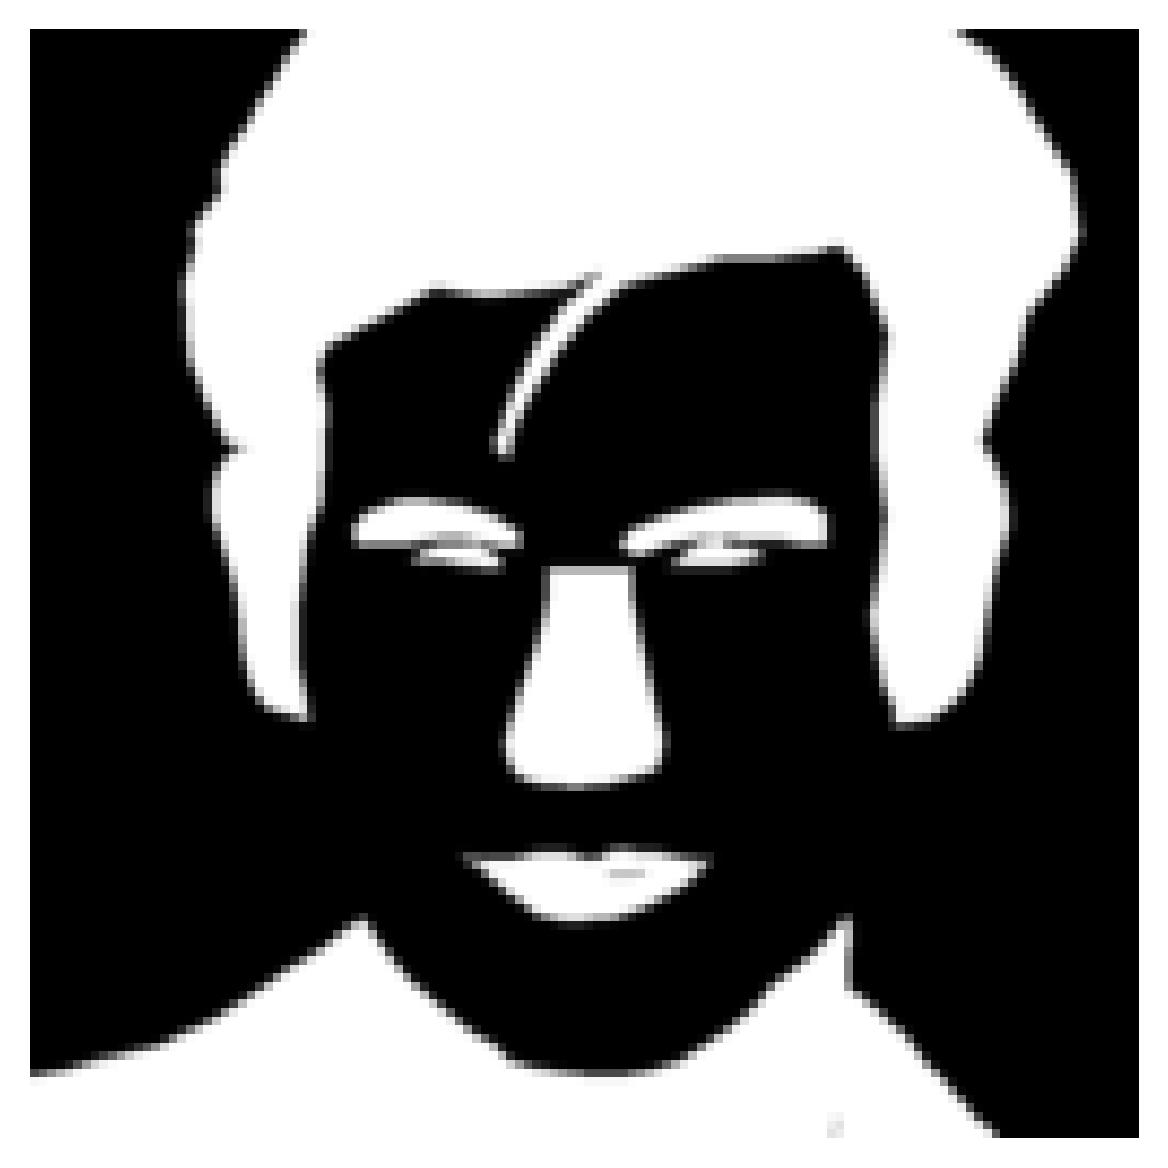
\includegraphics[width=\linewidth]{figures/datasets/celebA/examp5/5_mask_c.jpg}
         \caption*{ }
          \end{subfigure}
          
\end{subfigure}
  \begin{subfigure}{0.65\textwidth}
    \begin{subfigure}{1\textwidth}
 
         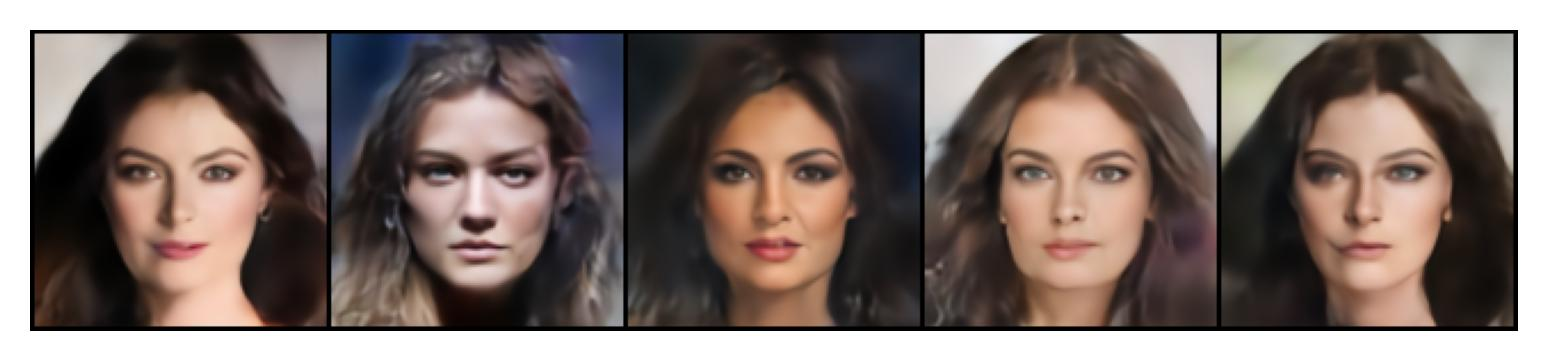
\includegraphics[width=\linewidth]{figures/datasets/celebA/im_cond_mask_attr_1.jpg}
    \end{subfigure}
    
     \begin{subfigure}{1\textwidth}
      
         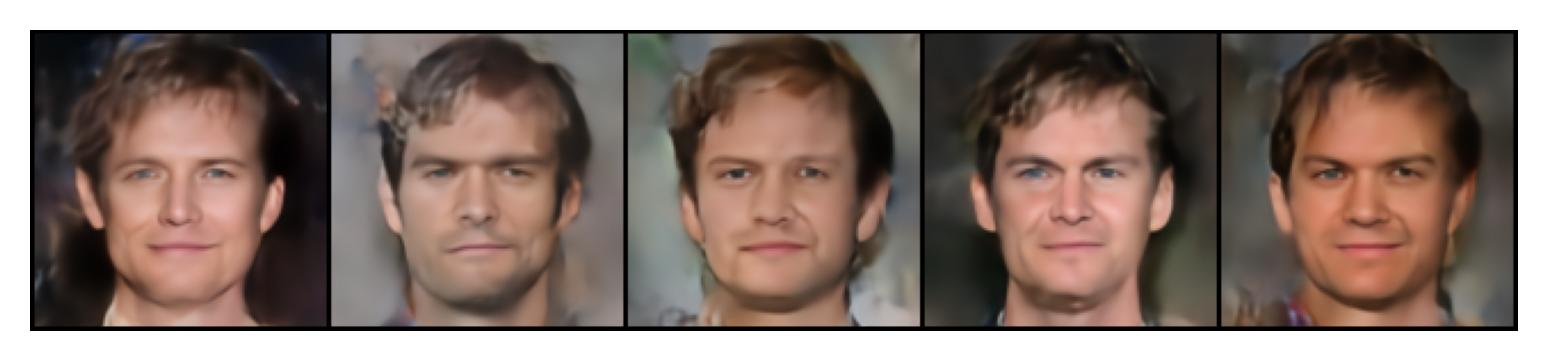
\includegraphics[width=\linewidth]{figures/datasets/celebA/examp2/2_im_cond_mask_attr_2.jpg}
    \end{subfigure}

    %  \begin{subfigure}{1\textwidth}
      
    %      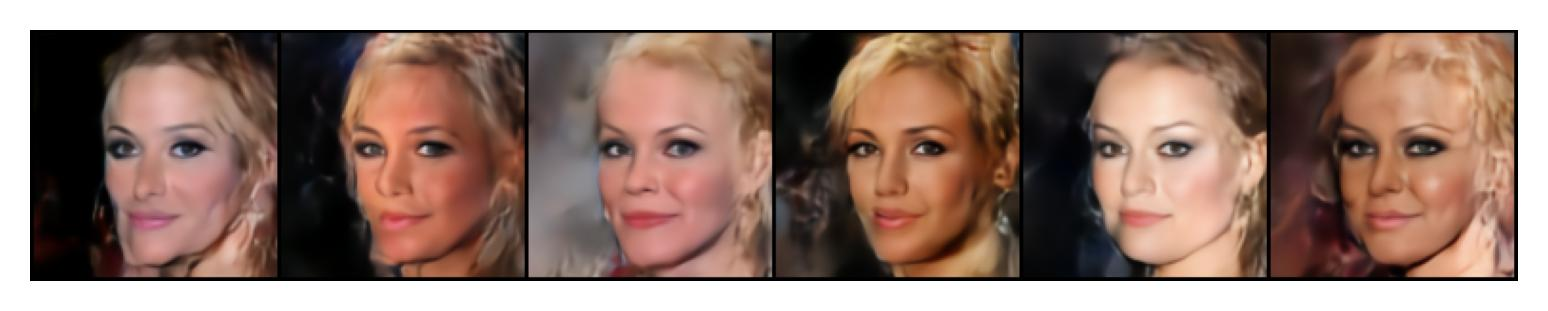
\includegraphics[width=\linewidth]{figures/datasets/celebA/examp3/3_im_cond_mask_att.jpg}
    % \end{subfigure}

     \begin{subfigure}{1\textwidth}
      
         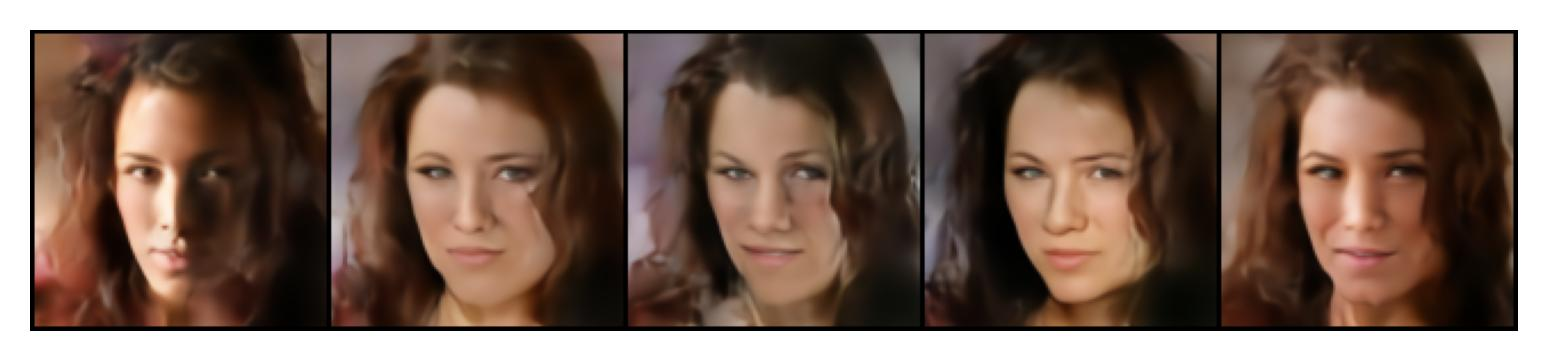
\includegraphics[width=\linewidth]{figures/datasets/celebA/examp4/4_im_cond_mask_attr_2.jpg}
    \end{subfigure}

       \begin{subfigure}{1\textwidth}
      
         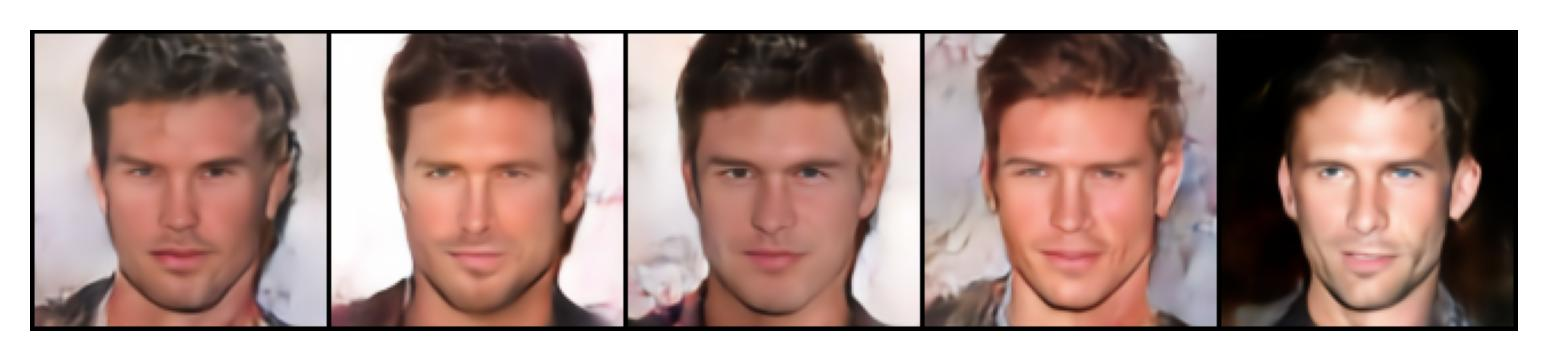
\includegraphics[width=\linewidth]{figures/datasets/celebA/examp5/5_im_cond_mask_att.jpg}
    \end{subfigure}
            \caption{Generated Images}
\end{subfigure}
        \caption{ (Attributes,Mask $\rightarrow$ Image ) Conditional generation of \textbf{\gls{MLD}} on CelebAMask-HQ.}
     
       
\end{figure}




\begin{figure}[H]
     \centering
     
     \begin{subfigure}{0.14\textwidth}
                \begin{subfigure}{1\textwidth}
         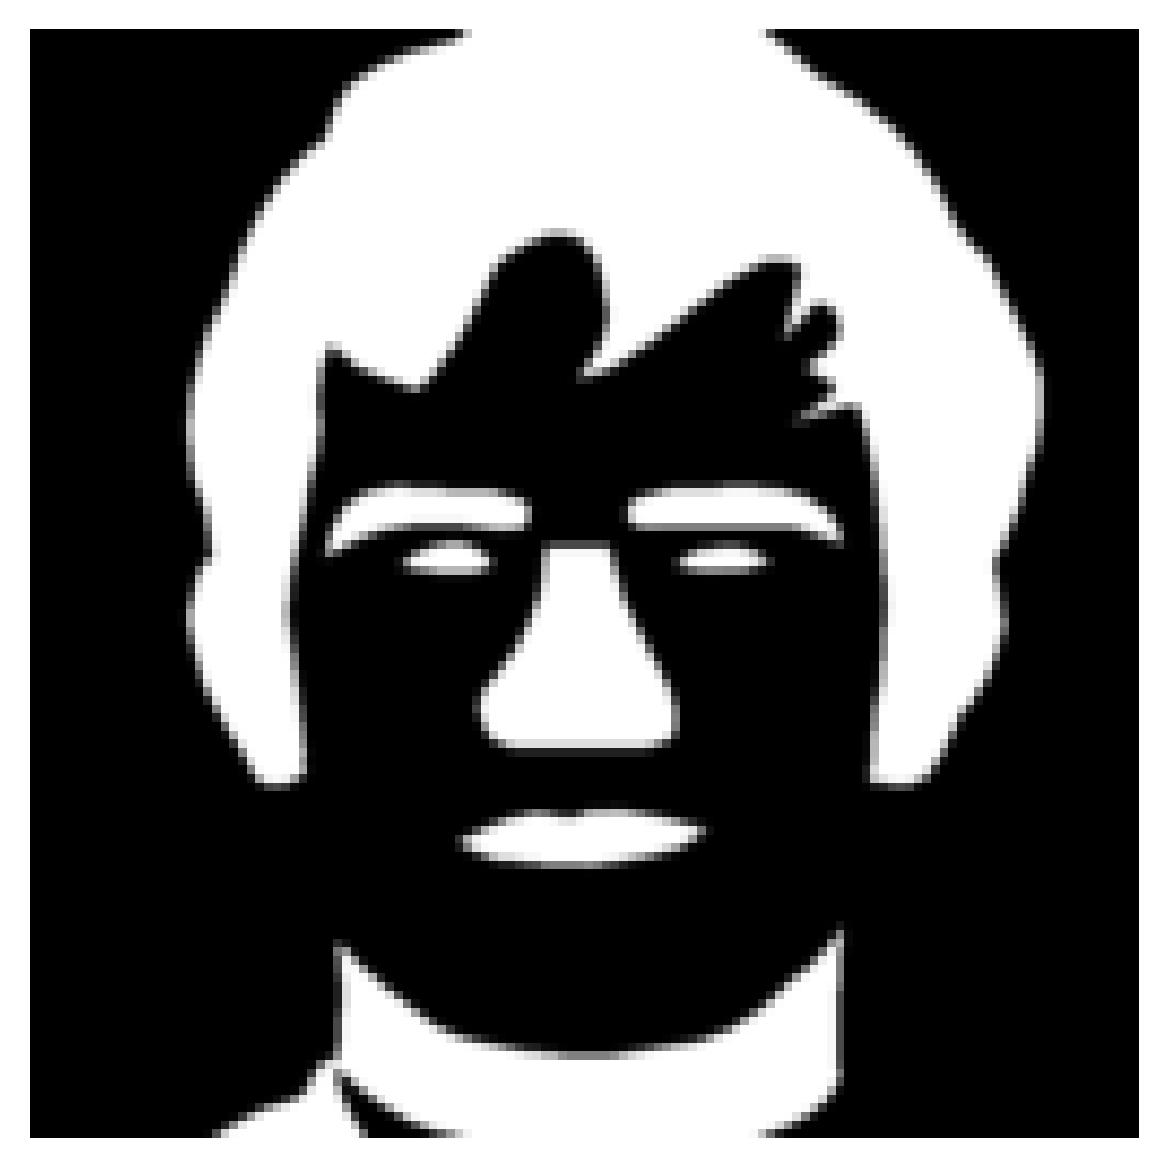
\includegraphics[width=\linewidth]{figures/datasets/celebA/examp2/2_mask_c.jpg}
          \end{subfigure}

               \begin{subfigure}{1\textwidth} 
         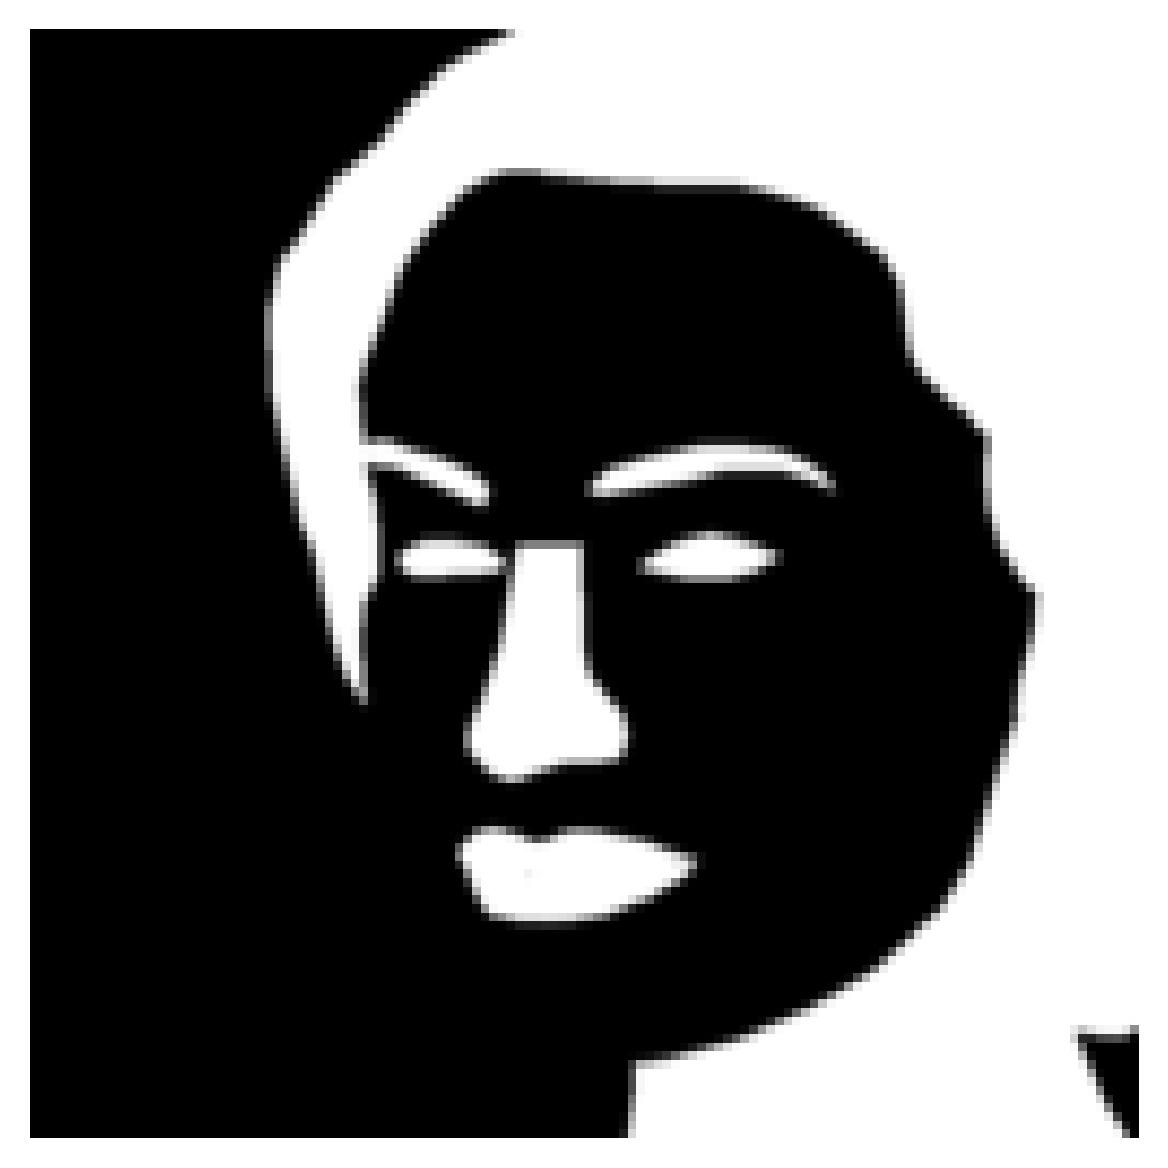
\includegraphics[width=\linewidth]{figures/datasets/celebA/examp3/3_mask_c.jpg}
          \end{subfigure}

             \begin{subfigure}{1\textwidth}
         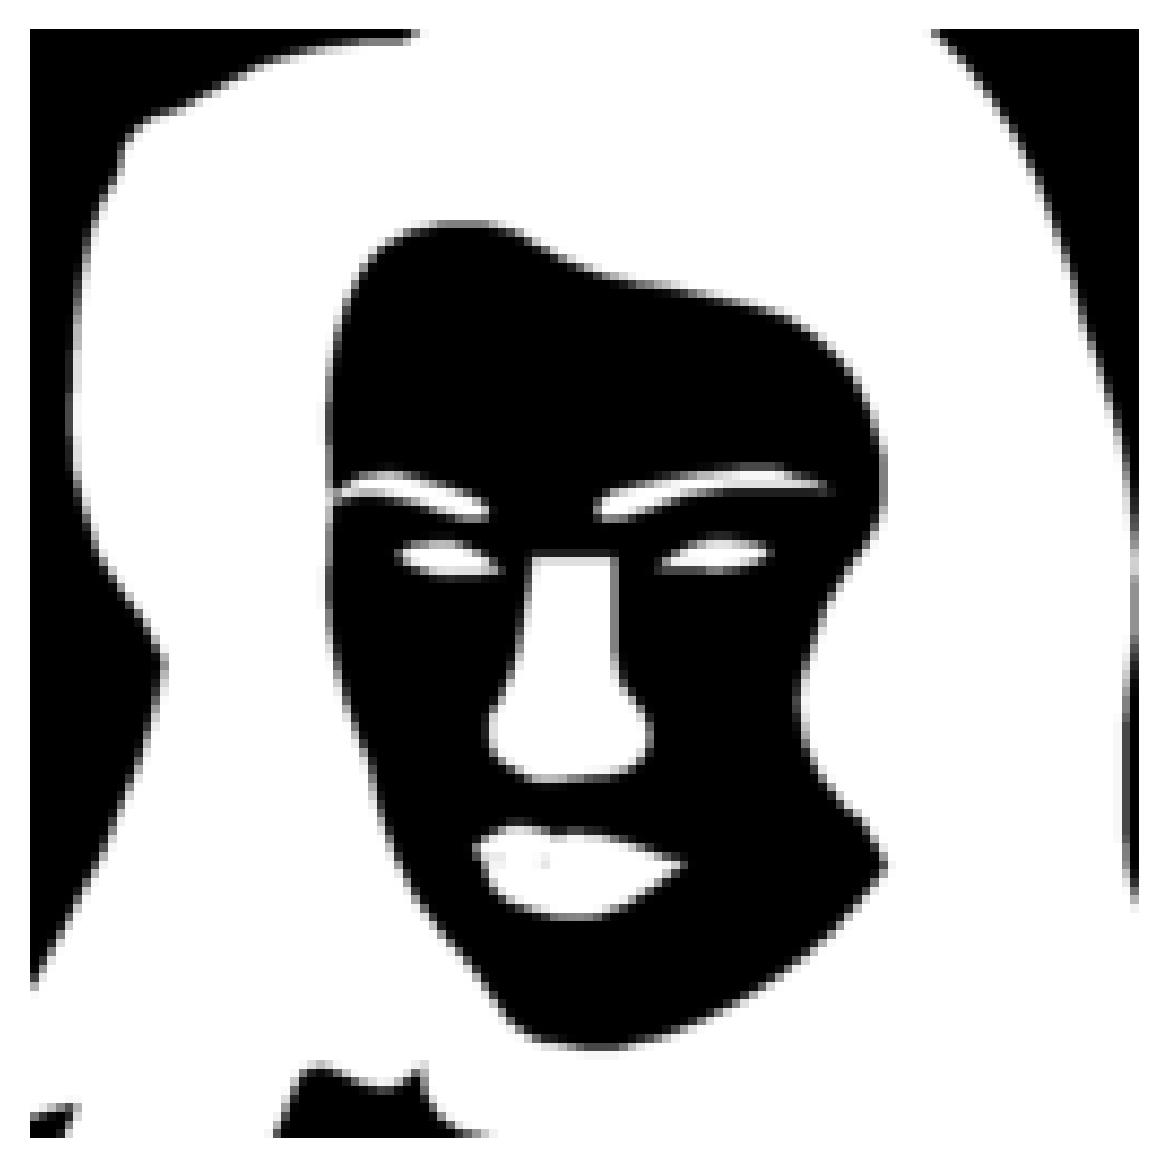
\includegraphics[width=\linewidth]{figures/datasets/celebA/examp4/4_mask_c.jpg}
          \end{subfigure}

                 \begin{subfigure}{1\textwidth}
         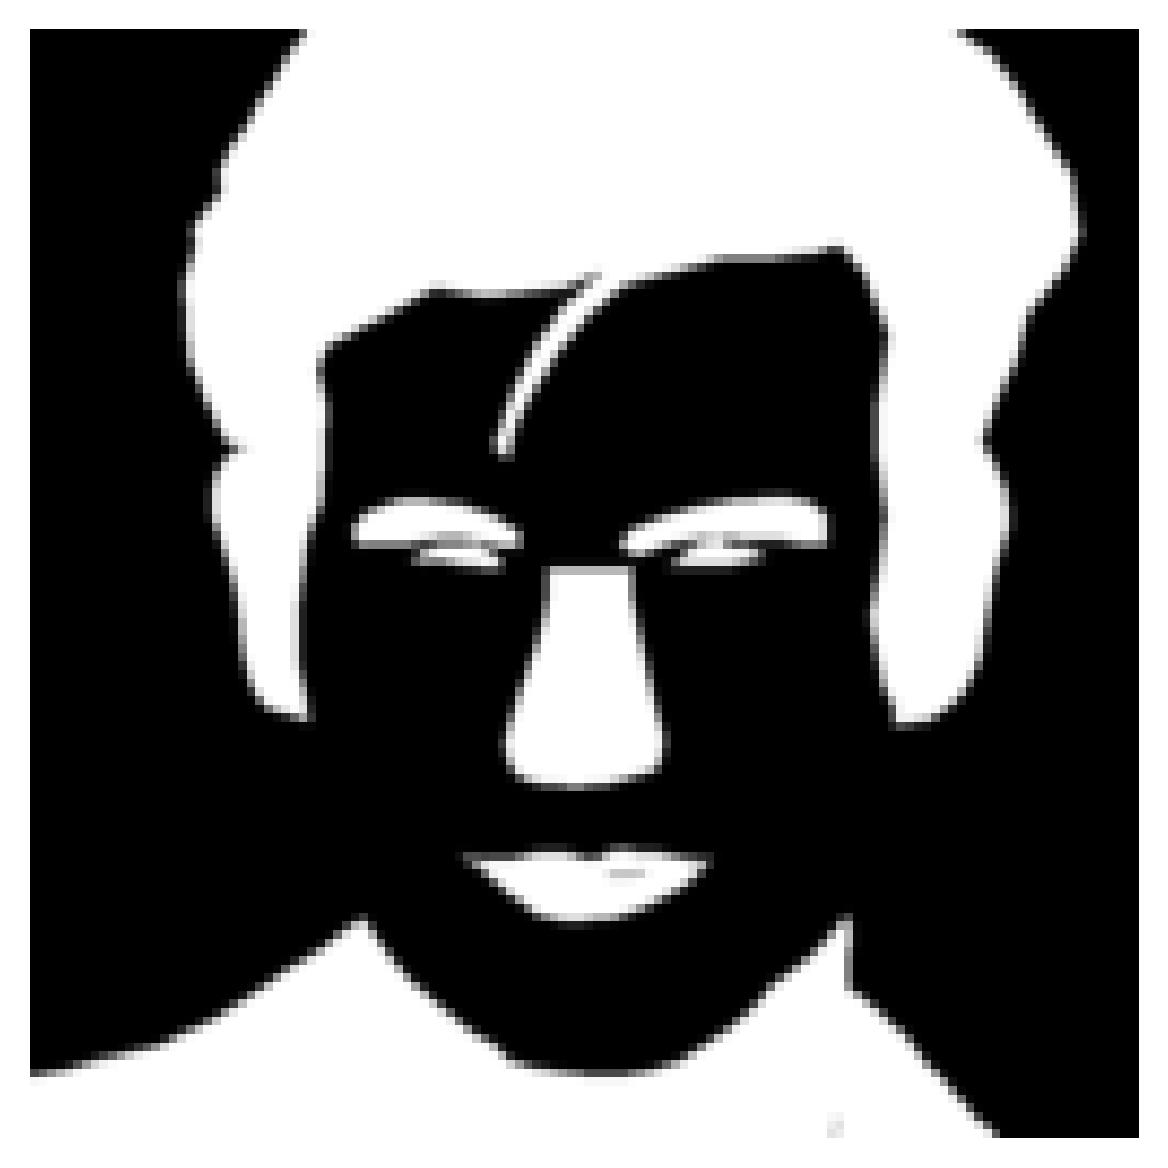
\includegraphics[width=\linewidth]{figures/datasets/celebA/examp5/5_mask_c.jpg}
         \caption*{ }
          \end{subfigure}
    \end{subfigure}
      \begin{subfigure}{0.14\textwidth}
      \end{subfigure}
  \begin{subfigure}{0.7\textwidth}
  
     \begin{subfigure}{1\textwidth}
      
         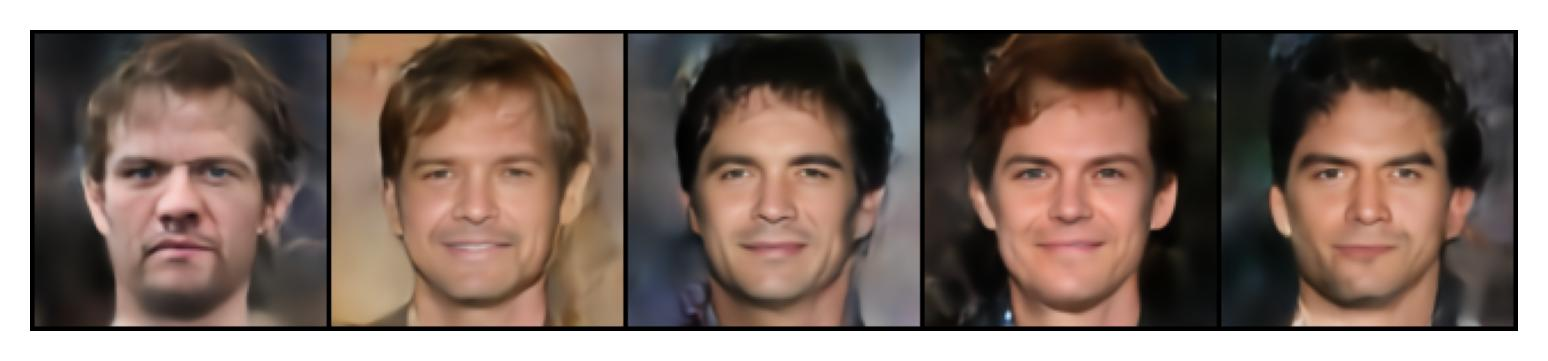
\includegraphics[width=\linewidth]{figures/datasets/celebA/examp2/2_im_cond_mask.jpg}
    \end{subfigure}

     \begin{subfigure}{1\textwidth}
      
         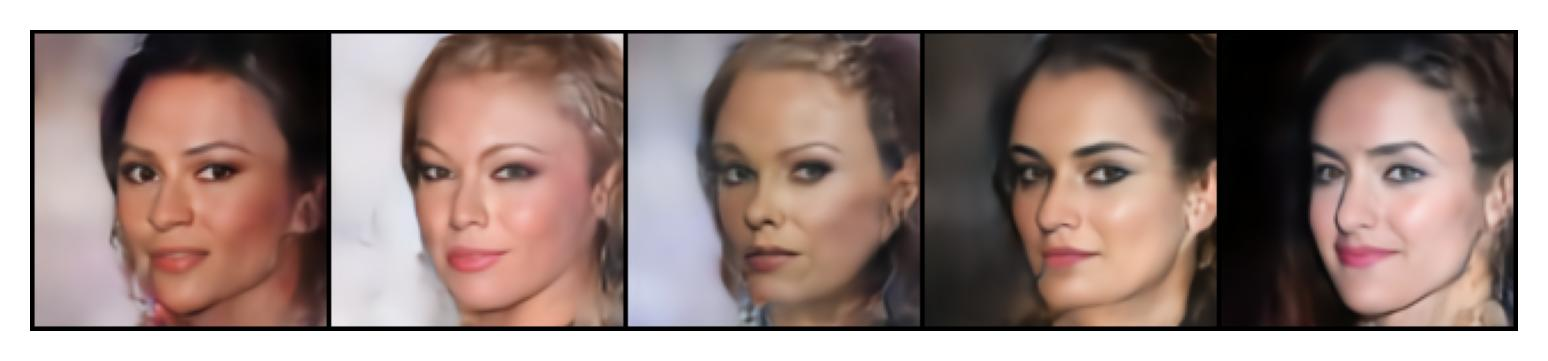
\includegraphics[width=\linewidth]{figures/datasets/celebA/examp3/3_im_cond_mask.jpg}
    \end{subfigure}

      \begin{subfigure}{1\textwidth}
      
         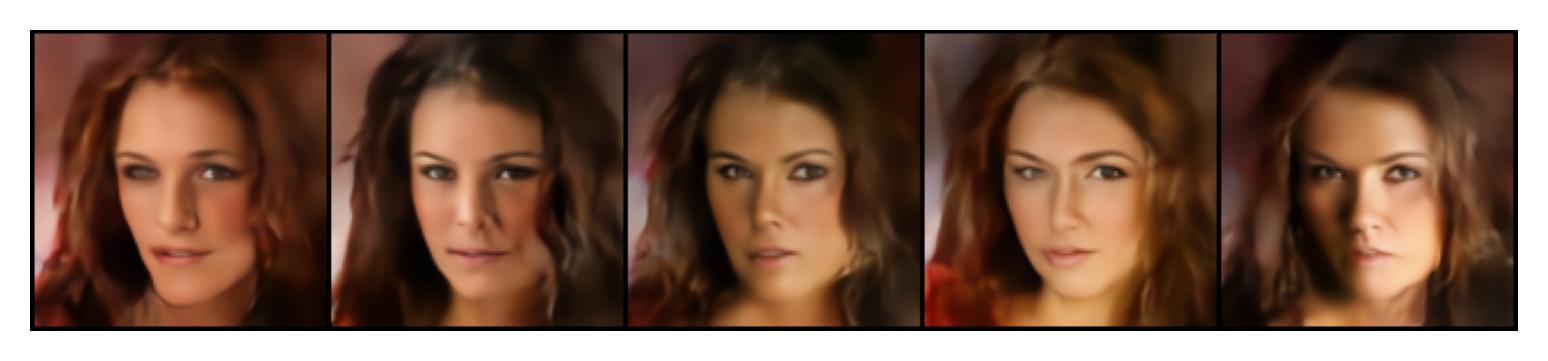
\includegraphics[width=\linewidth]{figures/datasets/celebA/examp4/4_im_cond_mask.jpg}
    \end{subfigure}

         \begin{subfigure}{1\textwidth}
    
         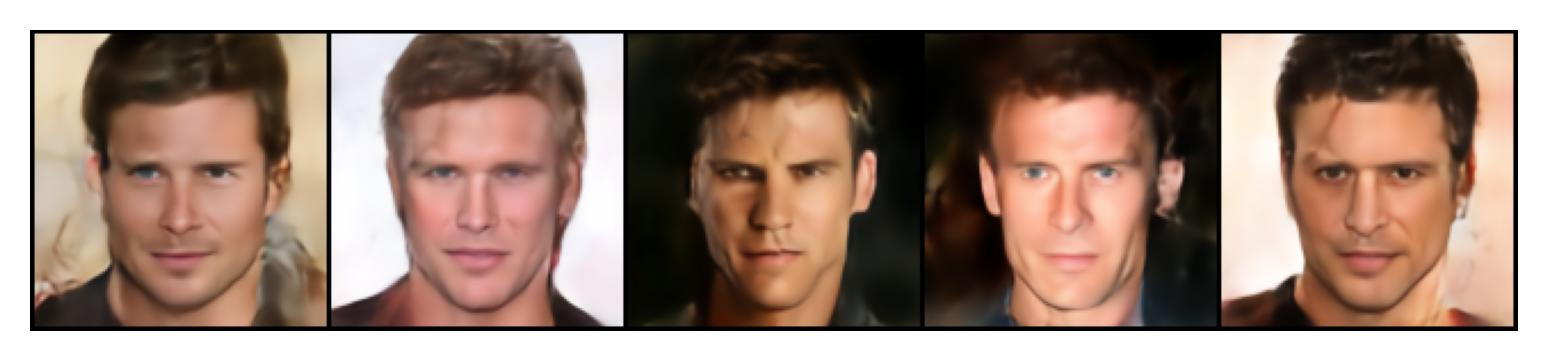
\includegraphics[width=\linewidth]{figures/datasets/celebA/examp5/5_im_cond_mask.jpg}
      
          \end{subfigure}
    
            \caption{Generated Images}
\end{subfigure}
        \caption{ (Mask $\rightarrow$ Image ) Conditional generation of \textbf{\gls{MLD}} on CelebAMask-HQ.}
     
       
\end{figure}






\begin{figure}[H]
     \centering
     
     \begin{subfigure}{0.14\textwidth}
       \centering
                \begin{subfigure}{1\textwidth}
    
         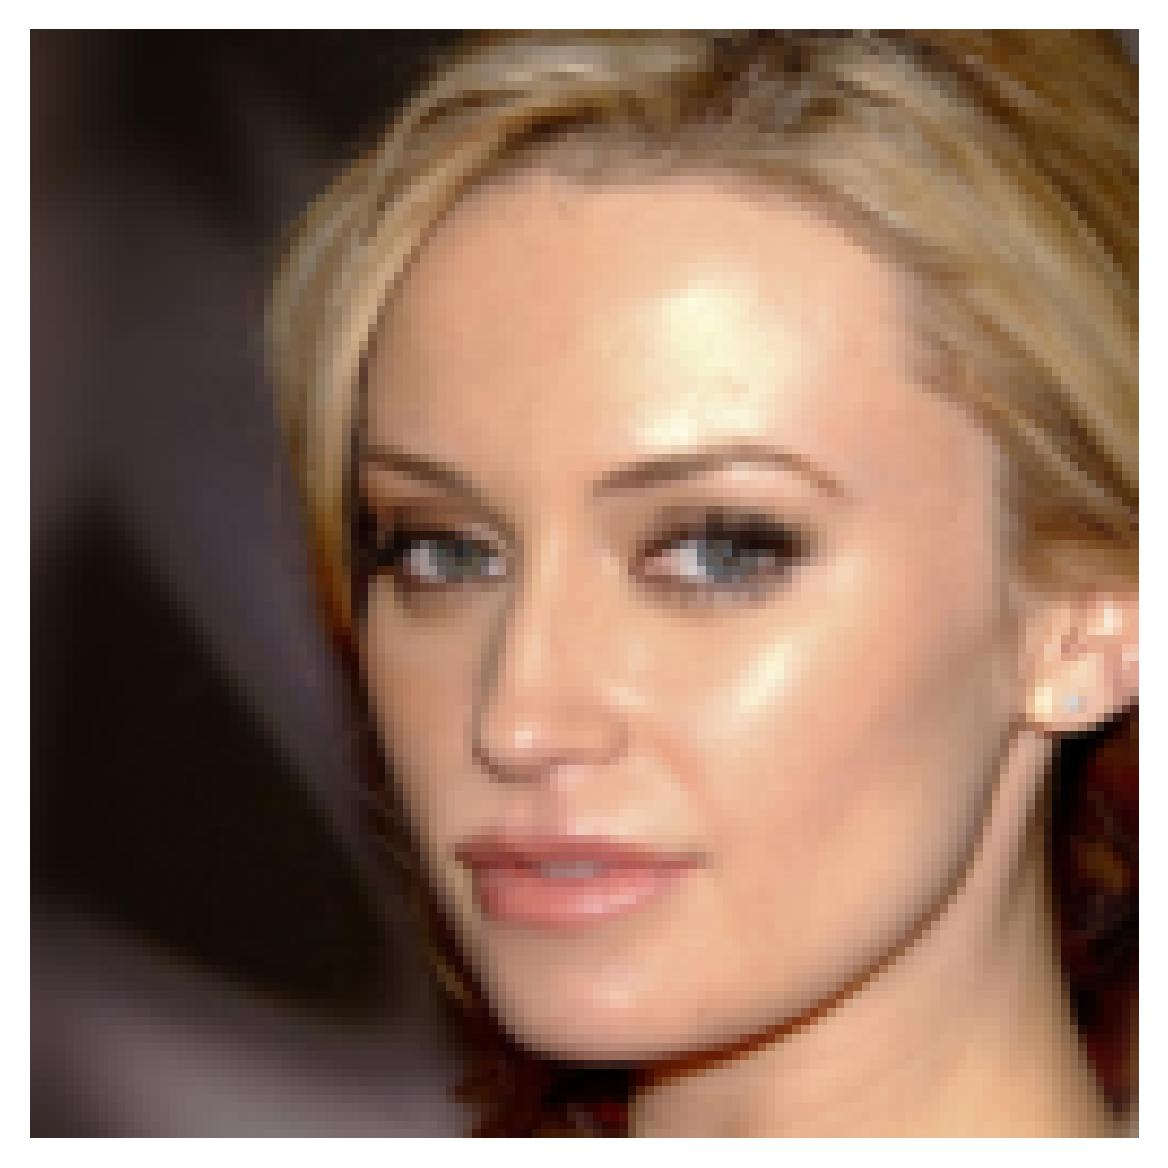
\includegraphics[width=\linewidth]{figures/datasets/celebA/examp3/3_image_c.jpg}
         \caption*{ }\end{subfigure}

\vspace{3pc}

         \begin{subfigure}{1\textwidth}
    
         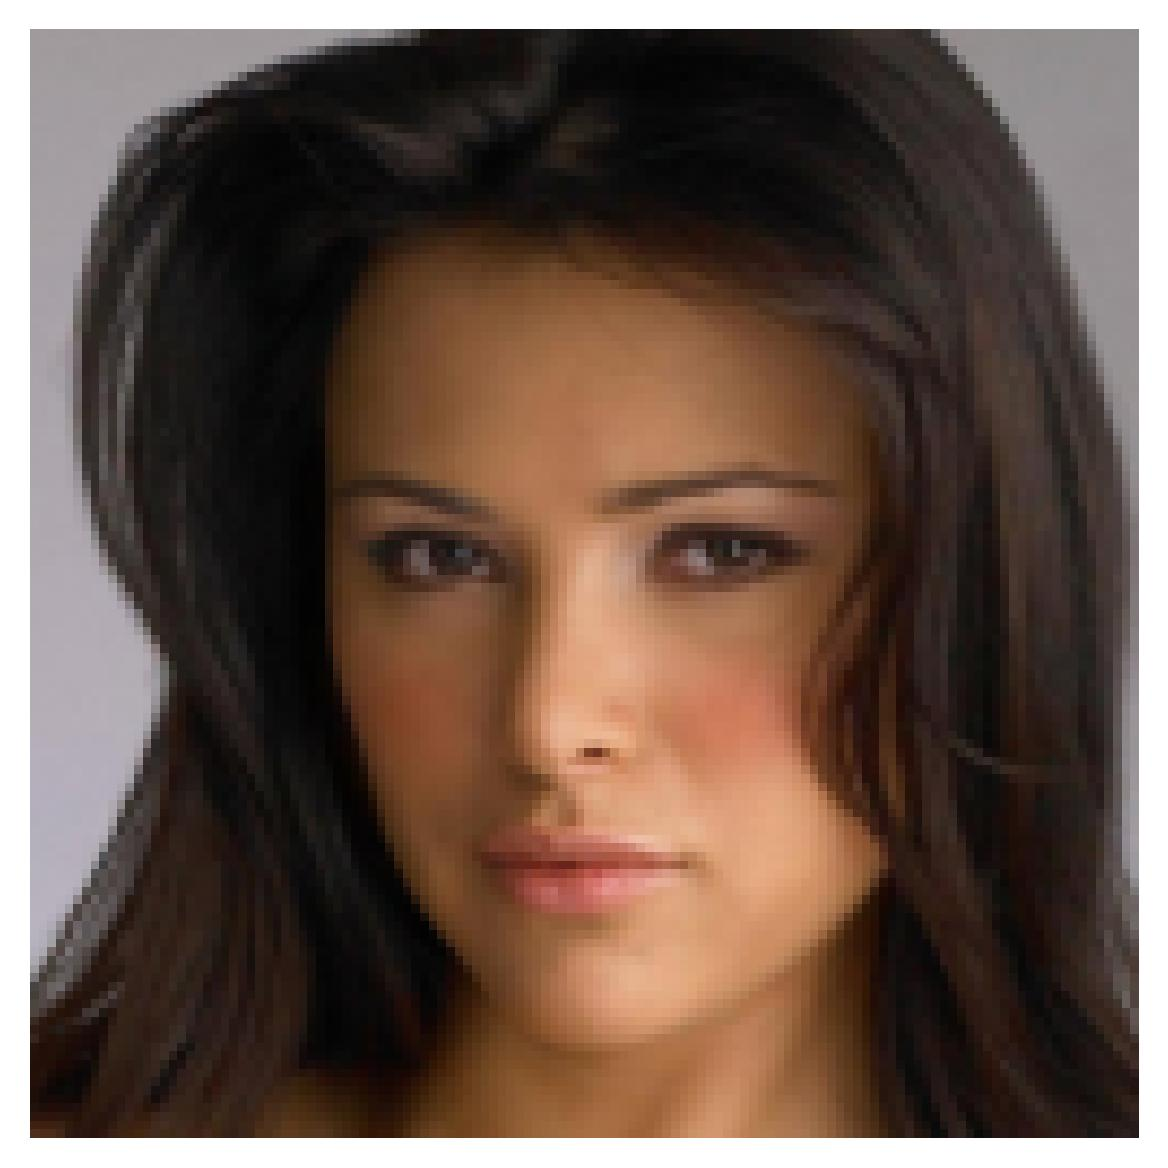
\includegraphics[width=\linewidth]{figures/datasets/celebA/examp4/4_image_c.jpg}
         \caption*{ }\end{subfigure}
         
\vspace{3pc}

              \begin{subfigure}{1\textwidth}
    
         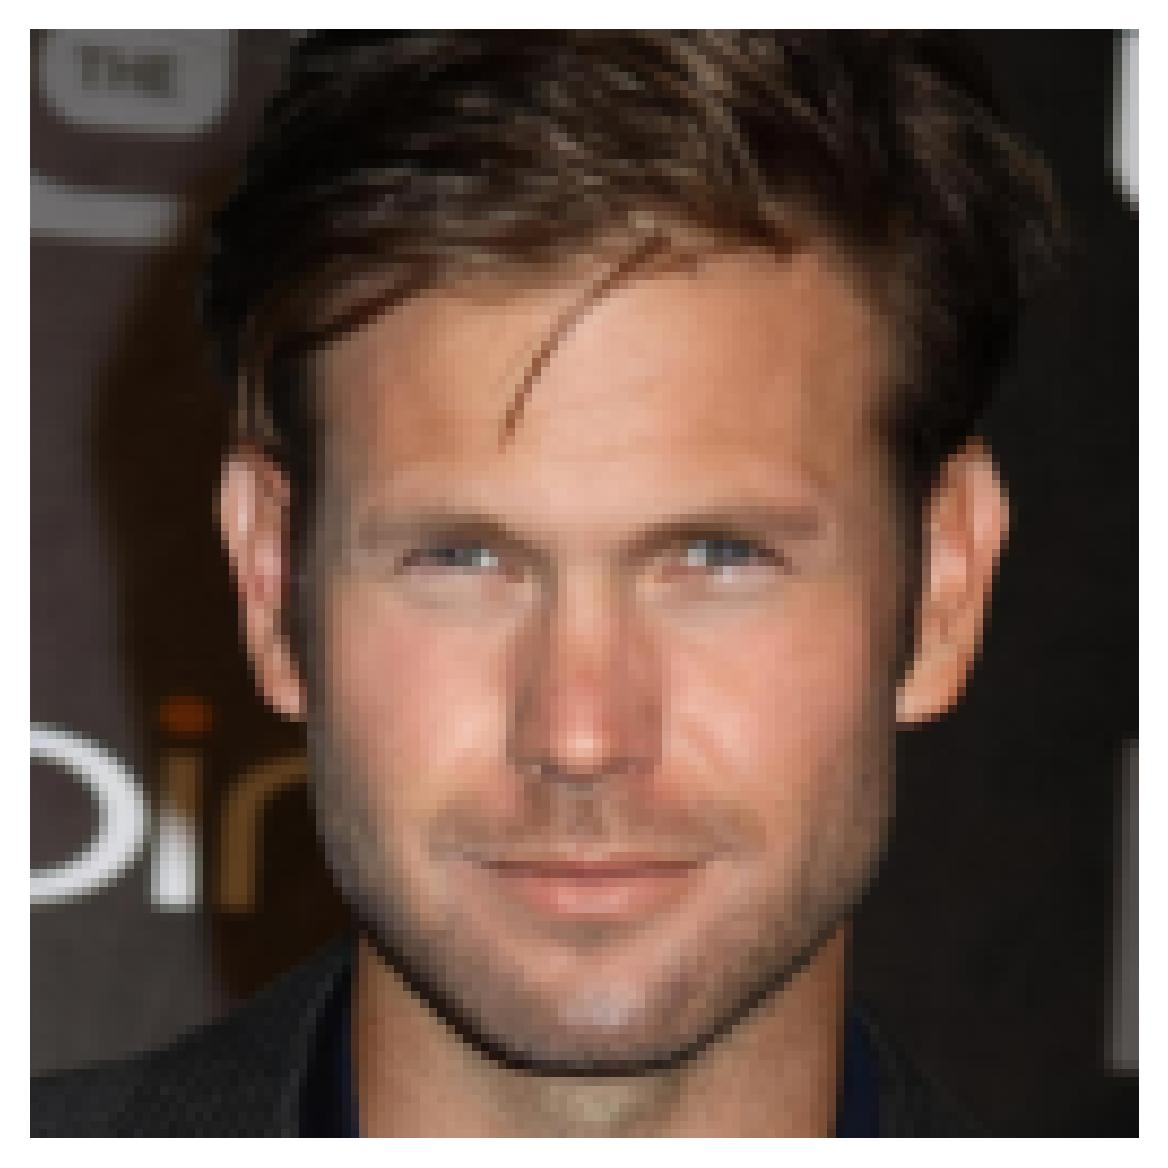
\includegraphics[width=\linewidth]{figures/datasets/celebA/examp5/5_image_c.jpg}
         \caption*{ }
          \end{subfigure}
         
          \end{subfigure}
\begin{subfigure}{0.5\textwidth}
    \begin{subfigure}{1\textwidth}
         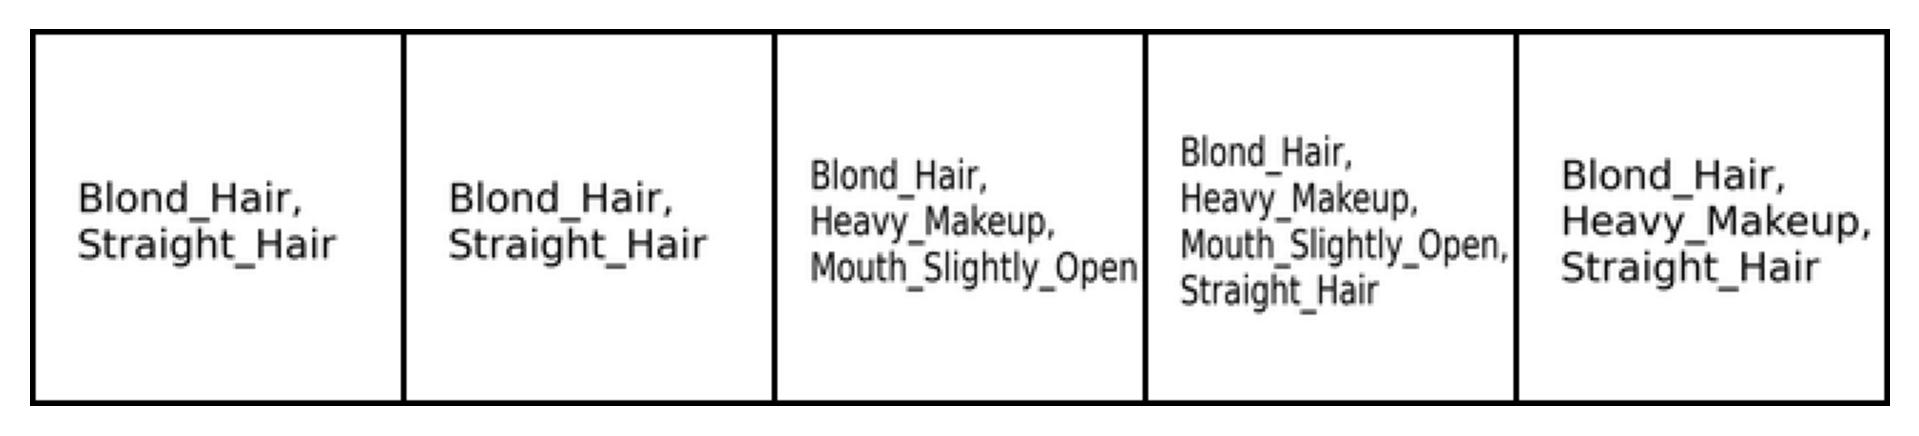
\includegraphics[width=\linewidth]{figures/datasets/celebA/examp3/3_attr_cond_im.jpg}
         \caption*{ }
          \end{subfigure}


   \begin{subfigure}{1\textwidth}
    
         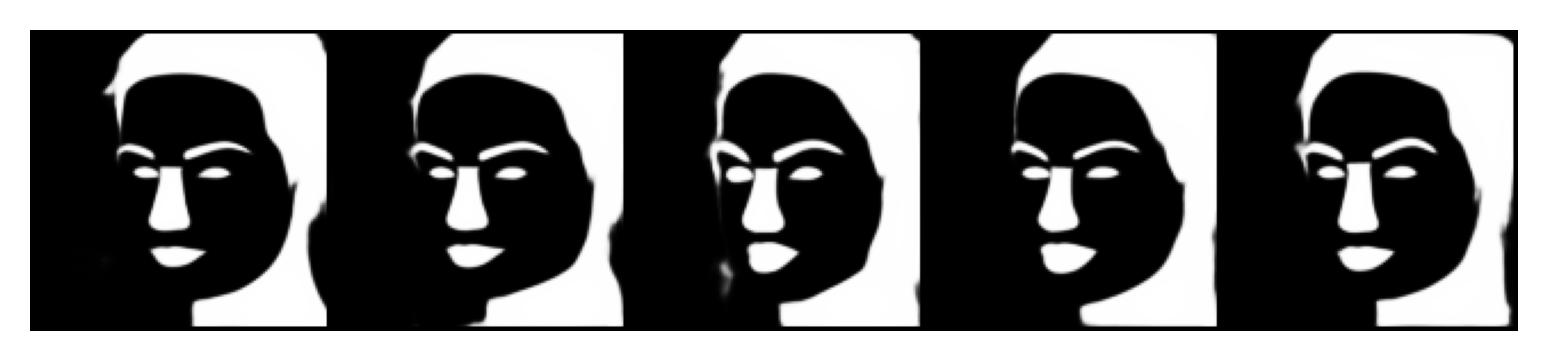
\includegraphics[width=\linewidth]{figures/datasets/celebA/examp3/3_mask_cond_im.jpg}
      


     \begin{subfigure}{1\textwidth}
         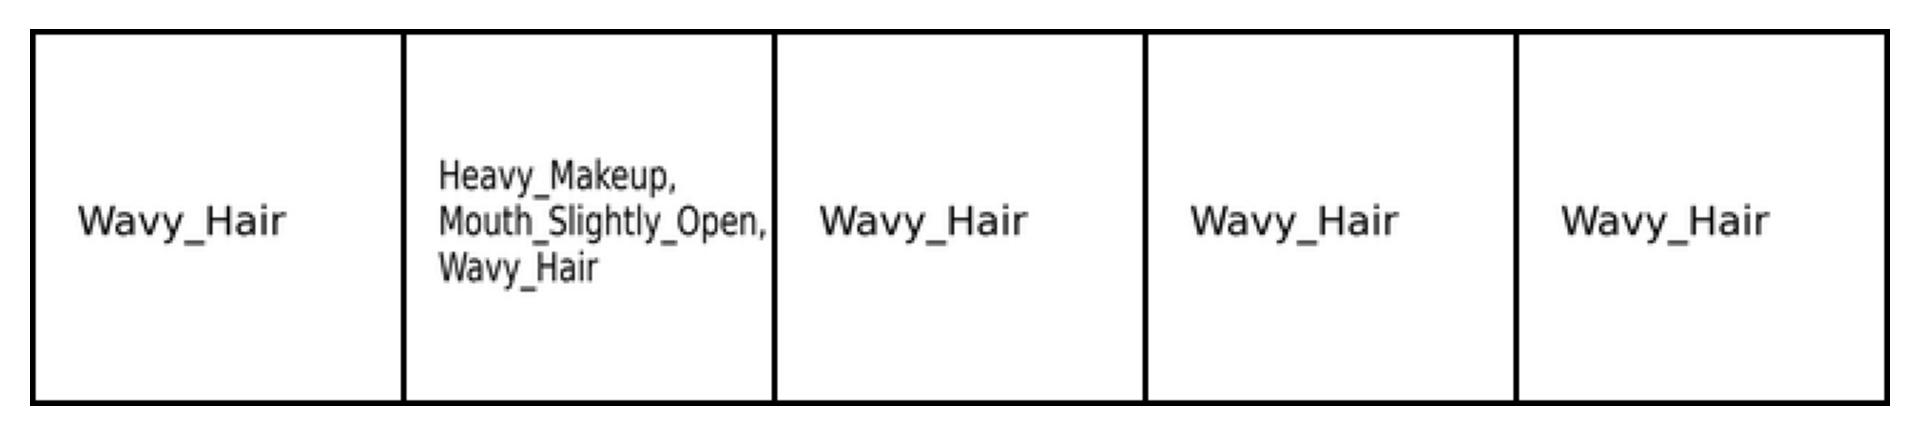
\includegraphics[width=\linewidth]{figures/datasets/celebA/examp4/4_attr_cond_im.jpg}
      
          \end{subfigure}


           \begin{subfigure}{1\textwidth}
         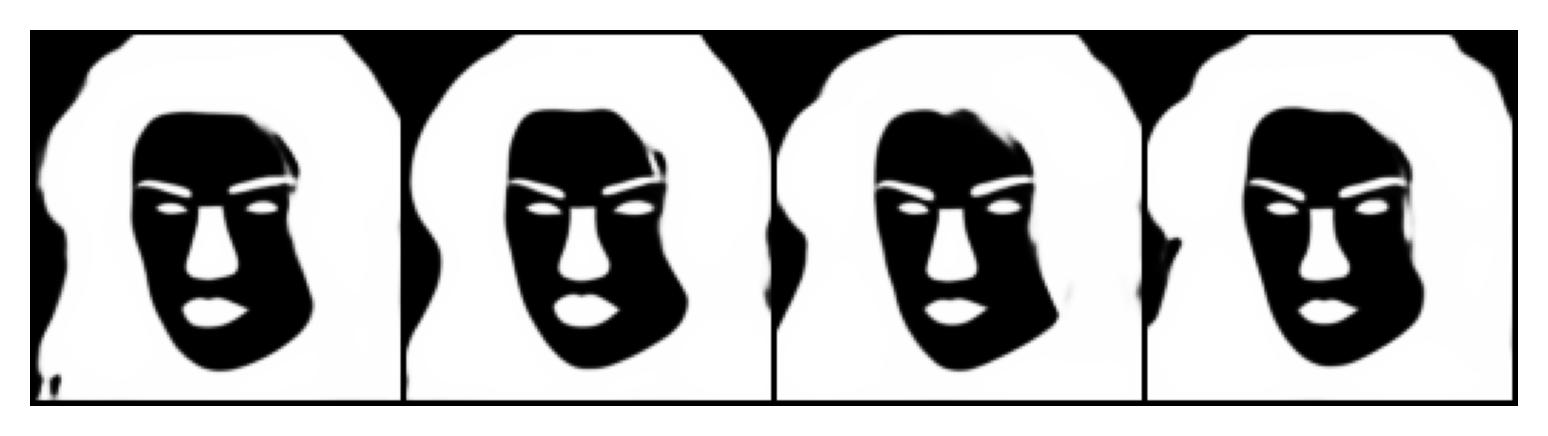
\includegraphics[width=\linewidth]{figures/datasets/celebA/examp4/4_mask_cond_im.jpg}
       
          \end{subfigure}



            \begin{subfigure}{1\textwidth}
         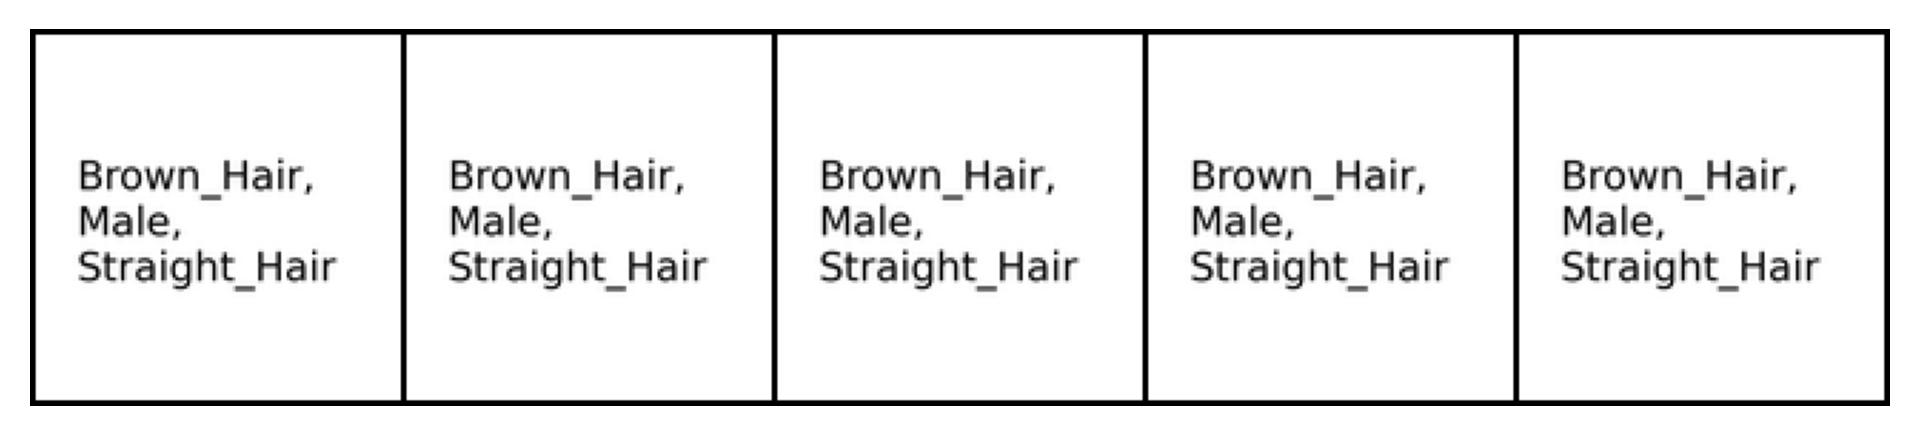
\includegraphics[width=\linewidth]{figures/datasets/celebA/examp5/5_attr_cond_im.jpg}
      
          \end{subfigure}

           \begin{subfigure}{1\textwidth}
         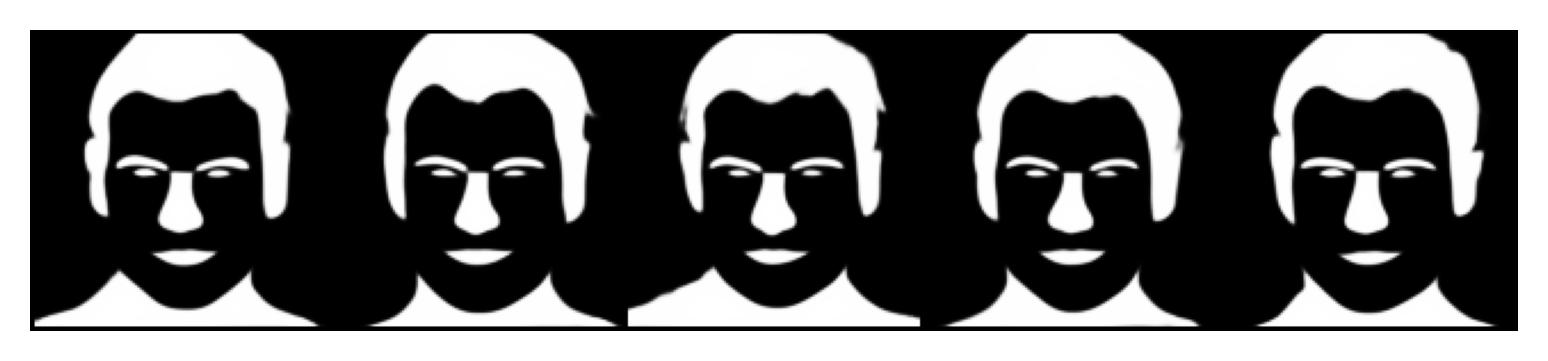
\includegraphics[width=\linewidth]{figures/datasets/celebA/examp5/5_mask_cond_im.jpg}
         \caption*{ }
          \end{subfigure}
          
          
    \end{subfigure}
\end{subfigure}




        \caption{ (Image $\rightarrow$ Attribute,Mask ) Conditional generation of \textbf{\gls{MLD}} on CelebAMask-HQ.}
      
       
\end{figure}